\documentclass{tufte-book}
%\documentclass[twoside,symmetric]{tufte-book}
\hypersetup{colorlinks}% uncomment this line if you prefer colored hyperlinks (e.g., for onscreen viewing)

%%
% Book metadata
\title{Introduction \\to Mechanics \thanks{Thanks to Edward R.~Tufte for his inspiration.}}
\author[The Tufte-LaTeX Developers]{Dr. Doeg}
\publisher{The Invisible College}

%%
% If they're installed, use Bergamo and Chantilly from www.fontsite.com.
% They're clones of Bembo and Gill Sans, respectively.
%\IfFileExists{bergamo.sty}{\usepackage[osf]{bergamo}}{}% Bembo
%\IfFileExists{chantill.sty}{\usepackage{chantill}}{}% Gill Sans

%\usepackage{microtype}

%%
% Just some sample text
\usepackage{lipsum}

%%
% For nicely typeset tabular material
\usepackage{booktabs}

%%
% For graphics / images
\usepackage{graphicx}
\setkeys{Gin}{width=\linewidth,totalheight=\textheight,keepaspectratio}
\graphicspath{{graphics/}}

%%
% Additional
\usepackage{units}
\usepackage{amsmath,amsfonts,amsthm} % Math packages
\usepackage{mathtools}% http://ctan.org/pkg/mathtools
%\usepackage{mparhack}
\usepackage{sectsty} % Allows customizing section commands
\usepackage[dvipsnames]{xcolor}
\usepackage{pgf,tikz}
\usepackage{pgfplots}
\usetikzlibrary{shapes,arrows}
\usetikzlibrary{patterns,fadings}
\usetikzlibrary{arrows}
 \usetikzlibrary{decorations.pathreplacing}
 \usetikzlibrary{decorations.markings}
 \usetikzlibrary{snakes}
 \usetikzlibrary{spy}
 \usepackage{setspace}
 \usepackage{3dplot}
 \usepackage{cancel}
\usepackage{physymb}
\usepackage{braket}
\usepackage{verbatim}
%\usepackage[x11names]{xcolor}                     %Additional colors
%\usepackage{euler}  



% The fancyvrb package lets us customize the formatting of verbatim
% environments.  We use a slightly smaller font.
\usepackage{fancyvrb}
\fvset{fontsize=\normalsize}

%%
% Prints argument within hanging parentheses (i.e., parentheses that take
% up no horizontal space).  Useful in tabular environments.
\newcommand{\hangp}[1]{\makebox[0pt][r]{(}#1\makebox[0pt][l]{)}}

%%
% Prints an asterisk that takes up no horizontal space.
% Useful in tabular environments.
\newcommand{\hangstar}{\makebox[0pt][l]{*}}

%%
% Prints a trailing space in a smart way.
\usepackage{xspace}

%%
% Some shortcuts for Tufte's book titles.  The lowercase commands will
% produce the initials of the book title in italics.  The all-caps commands
% will print out the full title of the book in italics.
\newcommand{\vdqi}{\textit{VDQI}\xspace}
\newcommand{\ei}{\textit{EI}\xspace}
\newcommand{\ve}{\textit{VE}\xspace}
\newcommand{\be}{\textit{BE}\xspace}
\newcommand{\VDQI}{\textit{The Visual Display of Quantitative Information}\xspace}
\newcommand{\EI}{\textit{Envisioning Information}\xspace}
\newcommand{\VE}{\textit{Visual Explanations}\xspace}
\newcommand{\BE}{\textit{Beautiful Evidence}\xspace}

\newcommand{\TL}{Tufte-\LaTeX\xspace}

% Prints the month name (e.g., January) and the year (e.g., 2008)
\newcommand{\monthyear}{%
  \ifcase\month\or January\or February\or March\or April\or May\or June\or
  July\or August\or September\or October\or November\or
  December\fi\space\number\year
}


% Prints an epigraph and speaker in sans serif, all-caps type.
\newcommand{\openepigraph}[2]{%
  %\sffamily\fontsize{14}{16}\selectfont
  \begin{fullwidth}
  \sffamily\large
  \begin{doublespace}
  \noindent\allcaps{#1}\\% epigraph
  \noindent\allcaps{#2}% author
  \end{doublespace}
  \end{fullwidth}
}

% Inserts a blank page
\newcommand{\blankpage}{\newpage\hbox{}\thispagestyle{empty}\newpage}

\usepackage{units}

% Typesets the font size, leading, and measure in the form of 10/12x26 pc.
\newcommand{\measure}[3]{#1/#2$\times$\unit[#3]{pc}}

% Macros for typesetting the documentation
\newcommand{\hlred}[1]{\textcolor{Maroon}{#1}}% prints in red
\newcommand{\hangleft}[1]{\makebox[0pt][r]{#1}}
\newcommand{\hairsp}{\hspace{1pt}}% hair space
\newcommand{\hquad}{\hskip0.5em\relax}% half quad space
\newcommand{\TODO}{\textcolor{red}{\bf TODO!}\xspace}
\newcommand{\ie}{\textit{i.\hairsp{}e.}\xspace}
\newcommand{\eg}{\textit{e.\hairsp{}g.}\xspace}
\newcommand{\na}{\quad--}% used in tables for N/A cells
\providecommand{\XeLaTeX}{X\lower.5ex\hbox{\kern-0.15em\reflectbox{E}}\kern-0.1em\LaTeX}
\newcommand{\tXeLaTeX}{\XeLaTeX\index{XeLaTeX@\protect\XeLaTeX}}
% \index{\texttt{\textbackslash xyz}@\hangleft{\texttt{\textbackslash}}\texttt{xyz}}
\newcommand{\tuftebs}{\symbol{'134}}% a backslash in tt type in OT1/T1
\newcommand{\doccmdnoindex}[2][]{\texttt{\tuftebs#2}}% command name -- adds backslash automatically (and doesn't add cmd to the index)
\newcommand{\doccmddef}[2][]{%
  \hlred{\texttt{\tuftebs#2}}\label{cmd:#2}%
  \ifthenelse{\isempty{#1}}%
    {% add the command to the index
      \index{#2 command@\protect\hangleft{\texttt{\tuftebs}}\texttt{#2}}% command name
    }%
    {% add the command and package to the index
      \index{#2 command@\protect\hangleft{\texttt{\tuftebs}}\texttt{#2} (\texttt{#1} package)}% command name
      \index{#1 package@\texttt{#1} package}\index{packages!#1@\texttt{#1}}% package name
    }%
}% command name -- adds backslash automatically
\newcommand{\doccmd}[2][]{%
  \texttt{\tuftebs#2}%
  \ifthenelse{\isempty{#1}}%
    {% add the command to the index
      \index{#2 command@\protect\hangleft{\texttt{\tuftebs}}\texttt{#2}}% command name
    }%
    {% add the command and package to the index
      \index{#2 command@\protect\hangleft{\texttt{\tuftebs}}\texttt{#2} (\texttt{#1} package)}% command name
      \index{#1 package@\texttt{#1} package}\index{packages!#1@\texttt{#1}}% package name
    }%
}% command name -- adds backslash automatically
\newcommand{\docopt}[1]{\ensuremath{\langle}\textrm{\textit{#1}}\ensuremath{\rangle}}% optional command argument
\newcommand{\docarg}[1]{\textrm{\textit{#1}}}% (required) command argument
\newenvironment{docspec}{\begin{quotation}\ttfamily\parskip0pt\parindent0pt\ignorespaces}{\end{quotation}}% command specification environment
\newcommand{\docenv}[1]{\texttt{#1}\index{#1 environment@\texttt{#1} environment}\index{environments!#1@\texttt{#1}}}% environment name
\newcommand{\docenvdef}[1]{\hlred{\texttt{#1}}\label{env:#1}\index{#1 environment@\texttt{#1} environment}\index{environments!#1@\texttt{#1}}}% environment name
\newcommand{\docpkg}[1]{\texttt{#1}\index{#1 package@\texttt{#1} package}\index{packages!#1@\texttt{#1}}}% package name
\newcommand{\doccls}[1]{\texttt{#1}}% document class name
\newcommand{\docclsopt}[1]{\texttt{#1}\index{#1 class option@\texttt{#1} class option}\index{class options!#1@\texttt{#1}}}% document class option name
\newcommand{\docclsoptdef}[1]{\hlred{\texttt{#1}}\label{clsopt:#1}\index{#1 class option@\texttt{#1} class option}\index{class options!#1@\texttt{#1}}}% document class option name defined
\newcommand{\docmsg}[2]{\bigskip\begin{fullwidth}\noindent\ttfamily#1\end{fullwidth}\medskip\par\noindent#2}
\newcommand{\docfilehook}[2]{\texttt{#1}\index{file hooks!#2}\index{#1@\texttt{#1}}}
\newcommand{\doccounter}[1]{\texttt{#1}\index{#1 counter@\texttt{#1} counter}}

% Generates the index
\usepackage{makeidx}
\makeindex

\begin{document}

% Front matter
\frontmatter

% r.1 blank page
%\blankpage

% v.2 epigraphs
\newpage\thispagestyle{empty}
\openepigraph{%
I think that modern physics has definitely decided in favor of Plato. In fact the smallest units of matter are not physical objects in the ordinary sense; they are forms, ideas which can be expressed unambiguously only in mathematical language.
}{Werner Heisenberg%, {\itshape Design, Form, and Chaos}
}
\vfill
\openepigraph{%
The only shibboleth the West has is science. It is the premise of modernity and it defines itself as a rationality capable of, indeed requiring separation from politics, religion and really, society. Modernisation is to work towards this\ldots If one looks at the works of Newton to Einstein, they were never scientists in the way modernity understands the term. 
}{Bruno Latour}
\vfill
\openepigraph{%
The boundary between science fiction and social reality is an optical illusion.
}{Donna Haraway}


% r.3 full title page
\maketitle


% v.4 copyright page
\newpage
\begin{fullwidth}
~\vfill
\thispagestyle{empty}
\setlength{\parindent}{0pt}
\setlength{\parskip}{\baselineskip}
Copyright \copyright\ \the\year\ \thanklessauthor

\par\smallcaps{Published by \thanklesspublisher}

\par\smallcaps{https://github.com/Trismeg/PhysicsBook}

\par Licensed under the Apache License, Version 2.0 (the ``License''); you may not
use this file except in compliance with the License. You may obtain a copy
of the License at \url{http://www.apache.org/licenses/LICENSE-2.0}. Unless
required by applicable law or agreed to in writing, software distributed
under the License is distributed on an \smallcaps{``AS IS'' BASIS, WITHOUT
WARRANTIES OR CONDITIONS OF ANY KIND}, either express or implied. See the
License for the specific language governing permissions and limitations
under the License.\index{license}

\par\textit{First printing, \monthyear}
\end{fullwidth}

% r.5 contents
\tableofcontents

\listoffigures

\listoftables

% r.7 dedication
\cleardoublepage
~\vfill
\begin{doublespace}
\noindent\fontsize{18}{22}\selectfont\itshape
\nohyphenation
Dedicated to the ghosts of the college and the spectral bodies of physics. 
% \mbox{Edward R.~Tufte} 
%and \mbox{Donald E.~Knuth}.
\end{doublespace}
\vfill
\vfill


% r.9 introduction
%\cleardoublepage
\chapter*{Note}

This physics text is an OpenSource academic project developed in abstraction by the Invisible College.  The manuscript is written in \LaTeX \ and makes use of the \doccls{tufte-book} and \doccls{tufte-handout} document classes.  

\vspace{2cm}

http://latex-project.org/ftp.html

https://git-scm.com/downloads

%%
% Start the main matter (normal chapters)
\mainmatter

\chapter{Introduction}
\label{ch:intro}

\textit{The limits of my language means the limits of my world.}  \\
\noindent\textbf{-Ludwig Wittgenstein}

\vspace{1cm}
\begin{marginfigure}%
  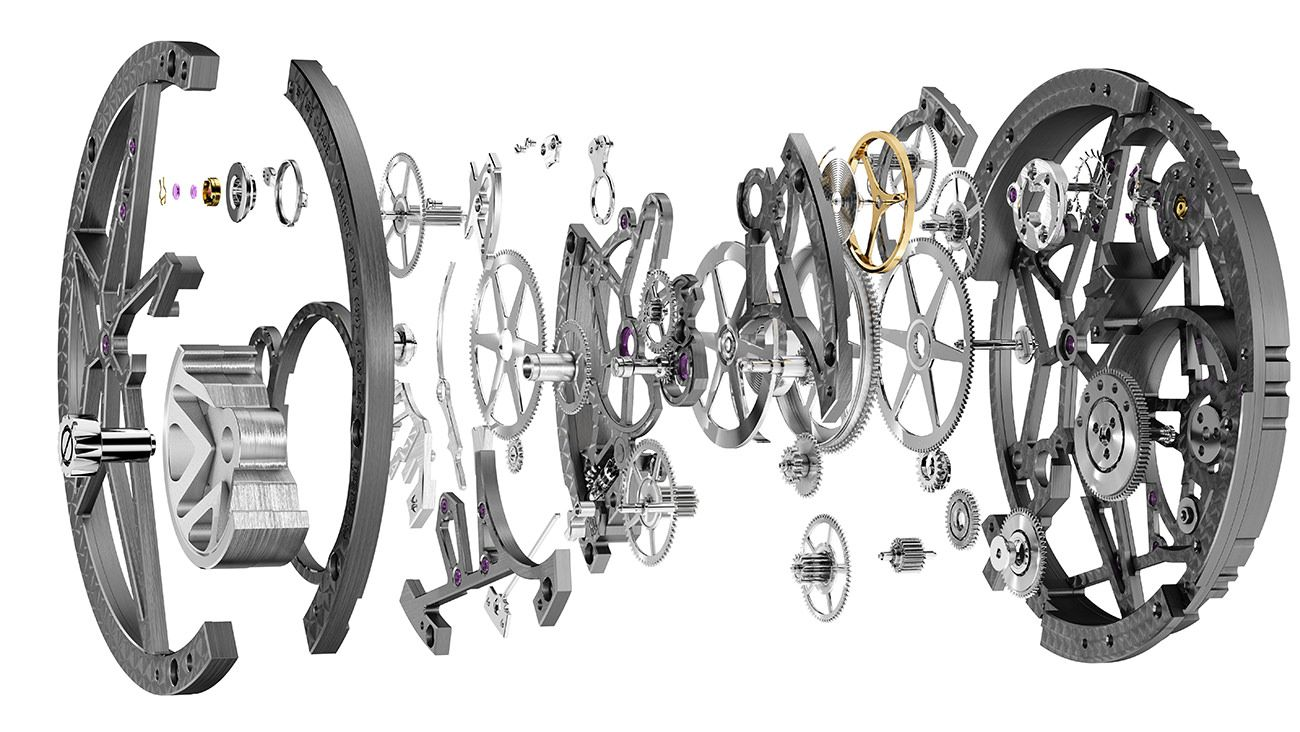
\includegraphics[width=\linewidth]{clock.jpg}
  \caption{Exploded clock assembly}
  \label{fig:marginfig}
\end{marginfigure}



\newthought{Physics is embodied} through the process of measurement.  Within physics any meaningful statement relates to some observable quantity.  The process of observation requires measurement using physical instrumentation.  In this way, physics is not only about the world but made of the world.
\begin{marginfigure}%
 \Large $$ E=hf$$
  \caption{Mathematical equation relating the energy and oscillatory frequency of a radiant particle.}
  \label{fig:marginfig}
\end{marginfigure}

\newthought{Physics is symbolic} in the application of mathematics to the working world.   Observable quantities are represented by algebraic variables and .  Once quantities are abstracted as mathematical variables, physics becomes a language game.

\newthought{Physics is visual} in both the measurement and the representation.
\begin{marginfigure}%
  \includegraphics[width=\linewidth]{bubble.jpg}
  \caption{Bubble chamber image of a neutrino particle interaction event from the Fermi National Accelerator Laboratory.}
  \label{fig:marginfig}
\end{marginfigure}
\newthought{Physics is social}.   In the end mathematics and physical observation are human activities.  As is Soylent Green, physics too is made of people.  People!  This does not mean we can not gain insights beyond ourselves.  Hopefully it means physicists will have jobs.
\begin{marginfigure}%
  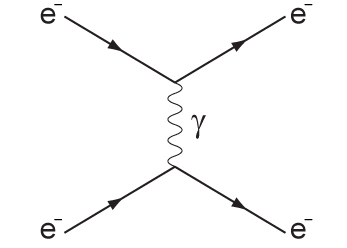
\includegraphics[width=\linewidth]{feyn.jpg}
  \caption{Feynman diagram representing photon mediated electron-electron scattering.}
  \label{fig:marginfig}
\end{marginfigure}

\section{Quantities}
\newthought{A physical quantity is} a physical property of a phenomenon, body, or substance, that can be quantified by measurement.  We can represent a physical quantity using an algebraic variable.  A physical quantity requires a value and unit of measure.
$$t = \overbrace{153}^{\textit{Value}} \ \ \overbrace{\text{seconds}}^{\textit{Unit}}$$
Consider the physical quantity, time.  In the above equation we use $t$ as the algebraic variable, seconds as the unit of measure and 153 as the value or magnitude of that unit.
\marginnote{\textit{So Simon Peter climbed back into the boat and dragged the net ashore. It was full of large fish, 153, but even with so many the net was not torn.}
\textbf{- John 21:11}}
\vspace{1cm}
$$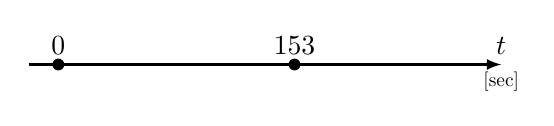
\begin{tikzpicture}[scale=1.5]
   \draw[->,thick,-latex] (0,0) -- (4,0) node [anchor=north ,scale=0.7] {$[\text{sec}]$}node [anchor=south ,scale=1] {$t $}; 
    %  \draw[->,-latex] (1.25,0.15) -- (2.75,0.15)  node [black,midway,above=0pt,yshift=2pt] { $\Delta_1 x_i$}; 
   \fill[black] (0.25,0) circle (0.5mm) node [anchor=south ,scale=1] {$0$};
    \fill[black] (2.25,0) circle (0.5mm) node [anchor=south ,scale=1] {$153$};
   
   \end{tikzpicture}
   $$
   \marginnote[-10pt]{The \textbf{accuracy} of a measurement system is the degree of closeness of measurements of a quantity to that quantity's true value.  The \textbf{precision} of a measurement system, related to reproducibility and repeatability, is the degree to which repeated measurements under unchanged conditions show the same results.}
The same information in the above equation may be encoded graphically using an appropriately labeled number line.  Here the quantity's magnitude may be represented a length measured by a point and the origin.

\subsection{Scientific Notation}
Scientific notation is a way of writing numbers that are too big or too small to be conveniently written in decimal form.  In scientific notation the numerical value 153 would be written as $1.53\times10^2$.

$$153= \overbrace{1.53}^{\text{significant figures}} \ \times\ \overbrace{10^2}^{\text{order of magnitude}}$$

In this format only one non-zero digit is to the left of the decimal place and to the right of the decimal place go the remaining significant figures.  The order of magnitude is the exponent power of ten.  In this example there are three significant figures and an order of magnitude of two.  Scientific notation enables simpler order-of-magnitude comparisons.


\begin{margintable}[20pt]\index{typefaces!sizes}
  \footnotesize%
  \begin{center}
    \begin{tabular}{lc}
      \toprule
     Length & Meters \\
      \midrule
     Observable Universe     & $10^{26}$  \\
    Milky Way      & $10^{21}$  \\
    Solar System     & $10^{13}$  \\
    Earth to Sun    & $10^{11}$  \\
    Earth     & $10^{7}$  \\
    Football Field      & $10^{2}$  \\
    Human      & $10^{0}$  \\
    Cell     & $10^{-5}$  \\
    Hydrogen Atom      & $10^{-10}$  \\
    Proton      & $10^{-15}$  \\
      \bottomrule
    \end{tabular}
  \end{center}
  \caption{A list of length scales.}
  \label{tab:font-sizes}
\end{margintable}

\begin{margintable}[20pt]\index{typefaces!sizes}
  \footnotesize%
  \begin{center}
    \begin{tabular}{lc}
      \toprule
     Time & Seconds\\
      \midrule
    Age Universe     & $10^{17}$  \\
    Age Earth      & $10^{17}$  \\
    Life on Earth      & $10^{17}$  \\
     Year    & $10^{7}$  \\
    Month    & $10^{6}$  \\
    Day     & $10^{5}$  \\
    Sunlight to Earth      & $10^{2}$  \\
    Heartbeat      & $10^{0}$  \\
    Audible Latency    & $10^{-2}$  \\
    Pion Lifetime      & $10^{-8}$  \\
      \bottomrule
    \end{tabular}
  \end{center}
  \caption{A list of time scales.}
  \label{tab:font-sizes}
\end{margintable}

\subsection{Approximation}
\newthought{Making order of magnitude approximations} involves using these $10^n$ representations.  Consider for example a deep breathing yogi.  How many breaths do they take per day?  The time scale for a breath is on the order of 10  or $(10^1)$ seconds while a day is on the order of $10^5$ seconds.  Therefore the number of breaths per day would be on the order of $10^4$, or ten thousand breaths.

$$\frac{10^5}{10^1}=10^{5-1}=10^4$$

Said another way, the time for the rotation of the earth is four orders of magnitude greater than the cycle of the breath.



\newpage
\subsection{Units and Dimensions}
\marginnote[20pt]{The \textit{International System of Units} (\textbf{SI}) is the modern form of the metric system and is the world's most widely used system of measurement, used in both commerce and science. It comprises a coherent system of units of measurement built on seven base units. It defines twenty-two named units, and includes many more unnamed coherent derived units. The system also establishes a set of twenty prefixes to the unit names and unit symbols that may be used when specifying multiples and fractions of the units.}


\begin{margintable}[20pt]\index{typefaces!sizes}
  \footnotesize%
  \begin{center}
    \begin{tabular}{lccl}
      \toprule
     Prefix & Symbol & Value \\
      \midrule
     yotta  & Y      & $10^{24}$  \\
    zetta  & Z      & $10^{21}$  \\
    exa    & E      & $10^{18}$  \\
    peta   & P      & $10^{15}$  \\
    tera   & T      & $10^{12}$  \\
    giga   & G      & $10^{9}$   \\
    mega   & M      & $10^{6}$   \\
    kilo   & k      & $10^{3}$   \\
    hecto  & h      & $10^{2}$   \\
    deca   & da     & $10^{1}$   \\ 
    deci   & d      & $10^{-1}$  \\
    centi  & c      & $10^{-2}$  \\
    milli  & m      & $10^{-3}$  \\
    micro  & $\mu\ $ & $10^{-6}$  \\
    nano   & n      & $10^{-9}$  \\
    pico   & p      & $10^{-12}$ \\
    femto  & f      & $10^{-15}$ \\
    atto   & a      & $10^{-18}$ \\
    zepto  & z      & $10^{-21}$ \\
    yocto  & y      & $10^{-24}$ \\
      \bottomrule
    \end{tabular}
  \end{center}
  \caption{A list of metric prefixes.}
  \label{tab:font-sizes}
\end{margintable}
\begin{description}
\item[meter] The meter is the length of the path travelled by light in vacuum during a tim interval of $1/299,792,458$ of a second.
\item[kilogram] The kilogram is the unit of mass; it is equal to the mass of the international prototype of the kilogram.
This international prototype is made of platinum-iridium and is kept at the International Bureau of Weights and Measures in France.
\item[second] The second is the duration of $9,192,631,770$ periods of the radiation corresponding
to the transition between the two hyper fine levels of the ground state of the cesium-133 atom.
\item[ampere] The ampere is that constant current which, if maintained in two straight parallel
conductors of infinite length, of negligible circular cross-section, and placed
one meter apart in vacuum, would produce between these conductors a force
equal to $2\times10^{-7}$ newton per meter of length.
\item[kelvin] The kelvin, unit of thermodynamic temperature, is the fraction 1/273.16 of the
thermodynamic temperature of the triple point of water.
\item[mole] The mole is the amount of substance of a system which contains as many
elementary entities as there are atoms in $0.012$ kilogram of carbon 12.  When the mole is used, the elementary entities must be specified and may be atoms, molecules, ions, electrons, other particles or specified groups of such particle.
In this definition, it is understood that the carbon 12 atoms are unbound, at rest and in their ground state.
\item[candela] The candela is the luminous intensity, in a given direction, of a source that emits
monochromatic radiation of a frequency $540\times10^{12}$ Hertz and has a radiant intensity in that direction of $1/683$ watt per steradian.
\end{description}



\begin{table}[htbp]
\begin{center}
\footnotesize
\begin{tabular}{lllll}
\toprule
Quantity & SI Unit & SI Symbol & Variable & Dimension  \\
\midrule
Fundamental & &  \\
\quad  distance & meter     & m           & $l$    &   $\mathbf{L}$          \\
\quad   mass &  kilogram  & kg          &      $m$       & $\mathbf{M}$        \\
\quad   time            & second    & s           &    $t$     &   $\mathbf{T}$      \\
\quad  electrical current &ampere &   A           &  $I$ &   $\mathbf{I}$    \\
\quad  temperature & kelvin    & K           &  $T$ &  $ \mathbf{\Theta} $ \\
\quad   number particles &   mole      & mol         &   $n$   &  $ \mathbf{N}$     \\
\quad  luminous intensity   & candela   & cd          &    $J$& $\mathbf{J}$      \\ \addlinespace
Derived & &  \\
\quad angle      &radian    & rad &$\theta$        &     $\mathbf{1}$           \\
\quad     frequency    &hertz     & Hz = $\nicefrac{1}{\text{s}}$         &      $f$ & $\mathbf{T}^{-1}$ \\
\quad    force & newton    & N   = $\nicefrac{\text{kg}\cdot \text{m}}{\text{s}^2}$        & $F$ & $\mathbf{M}\mathbf{L}\mathbf{T}^{-2}$           \\
\quad  pressure &  pascal    & Pa  = $\nicefrac{\text{N}}{\text{m}^2}$        &     $P$   & $\mathbf{M}\mathbf{L}^{-1}\mathbf{T}^{-2}$  \\
\quad   energy        &  joule     & J   = $\text{N} \cdot \text{m}$        &     $E$ & $\mathbf{M}\mathbf{L}^{2}\mathbf{T}^{-2}$\\
\quad    power       & watt      & W  = $\nicefrac{\text{J}}{\text{s}}$         &     $P$ & $\mathbf{M}\mathbf{L}^{2}\mathbf{T}^{-3}$  \\
\quad    electric charge  & coulomb   & C = $\text{A} \cdot \text{s}$           &   $q$& $\mathbf{I}\mathbf{T}$\\
\quad    electric potential & volt      & V = $\nicefrac{\text{J}}{\text{C}}$           & $V$& $\mathbf{M}\mathbf{L}^{2}\mathbf{T}^{-3}\mathbf{I}^{-1}$\\
 \quad  capacitance     & farad     & F = $\nicefrac{\text{C}}{\text{V}}$          &     $C$  & $\mathbf{M}^{-1}\mathbf{L}^{-2}\mathbf{T}^{4}\mathbf{I}^{2}$\\
 \quad   resistance   &ohm       & $\Omega$ = $\nicefrac{\text{V}}{\text{A}}$   &     $R$  & $\mathbf{M}\mathbf{L}^{2}\mathbf{T}^{-3}\mathbf{I}^{-2}$\\
 \quad   magnetic field    & tesla     & T  = $\nicefrac{\text{V}\cdot \text{s}}{\text{m}^2}$         & $B$   & $\mathbf{M}\mathbf{T}^{-2}\mathbf{I}^{-1}$ \\
\quad    inductance    & henry     & H = $\nicefrac{\text{V}\cdot \text{s}}{\text{A}}$         &   $L$ & $\mathbf{M}\mathbf{L}^{2}\mathbf{T}^{-2}\mathbf{I}^{-2}$ \\
 \quad  radioactivity  & becquerel & Bq = $\nicefrac{1}{\text{s}}$           & $A$  & $\mathbf{T}^{-1}$   \\ 
\bottomrule
\end{tabular}
\end{center}
  \caption{A list of physical quantities with SI units and dimensions.}
  \label{tab:font-sizes}
\end{table}

\newpage
\newthought{Any physical quantity} $Q$ is proportional to a product of fundamental quantities.  The critical exponents always being integer values.
 $$Q=Cl^\alpha m^\beta t^\gamma I^\delta T^\epsilon n^\xi J^\eta$$
\marginnote[-150pt]{The concept of physical dimension was introduced by Joseph Fourier in 1822.  Physical quantities that are commensurable have the same dimension; if they have different dimensions, they are incommensurable. For example, it is meaningless to ask whether a kilogram is less, the same, or more than an hour.  Any physically meaningful equation will have the same dimensions on the left and right sides, a property known as "dimensional homogeneity".}
The dimension of the quantity, $\text{dim }Q$, is a product of the dimensions of the constituent quantity factors.  
 $$\text{dim }Q=\mathbf{L}^\alpha \mathbf{M}^\beta \mathbf{T}^\gamma \mathbf{I}^\delta \mathbf{\Theta}^\epsilon \mathbf{N}^\xi \mathbf{J}^\eta$$
 \marginnote[-30pt]{Here $\alpha$, $\beta$, $\gamma$, $\delta$, $\epsilon$, $\xi$, $\eta$ are all positive or negative integers}
 This constitutes what is called and Abelian group.
 
\paragraph{Algebra and Similitude}
A sum or difference of two commensurate quantities (having the same dimensions) is a physically meaningful expression.
$$402\   \text{meter} -137\   \text{meter}=(402-137) \text{meter}=265\  \text{meter}$$
A product or quotient of any quantities can be a physically meaningful expression.
$$\frac{265\ \text{meter}}{153\ \text{second}}=\frac{265}{153}\ \frac{\text{meter}}{\text{second}}=1.73\  \nicefrac{\text{m}}{\text{s}}%\approx \sqrt{3}\ \nicefrac{\text{m}}{\text{s}}
$$

\paragraph{Unit Conversion}
\marginnote[-120pt]{The conversion of a quarter mile into meters.
\begin{align*} 
0.25\  \text{mi } \underbrace{\left(\frac{1609 \text{ m} }{ 1 \text{ mi}}\right)}_{\large{1}}&=\frac{0.25\cdot 1609}{1} \  \cancel{\text{mi}} \frac{\text{m} }{\cancel{\text{mi}}} \\
0.25\  \text{mi } &=402 \text{ m}
\end{align*}
}
\begin{margintable}[-30pt]\index{typefaces!sizes}
  \footnotesize%
  \begin{center}
    \begin{tabular}{lccl}
      \toprule
     English $\Longleftrightarrow$ Metric                                             \\
      \midrule
    $1 \text{ mile} = 5280 \text{ feet} = 1609 \text{ meters}$  \\
    $1 \text{gallon} = 3.785 \text{ liters} = 4.000 \text{ quarts}$                \\
    $1 \text{ cm}^3= 1 \text{ milliliter}$                                         \\
    $1 \text{ hp} = 746 \text{ Watts}$                                             \\
    $1 \text{ lb} = 4.45 \text{ Newtons}$                                          \\ 
      \bottomrule
    \end{tabular}
  \end{center}
  \caption{English and Metric equivalences}
  \label{tab:font-sizes}
\end{margintable}



The dimensions of a conversion factor are unity.  Any physically meaningful equality can be turned into one of two conversion factors.
$$1 \text{ mile} = 1609 \text{ meters} \ \ \ \ \ \Longleftrightarrow \ \ \ \ \ \frac{1609 \text{ meters} }{ 1 \text{ mile}}=\frac{ 1 \text{ mile}}{1609 \text{ meters} }=1$$






\newpage

\section{Constants}
\newthought{A physical constant is} a physical quantity that is generally believed to be both universal in nature and constant in time. It can be contrasted with a mathematical constant, which is a fixed numerical value, but does not directly involve any physical measurement.

\begin{table}[htbp]
\begin{center}
\footnotesize
\begin{tabular}{lllll}
\toprule
Earth                                     & Sun \& Moon                              & Water                                                                        \\
\midrule
 $g=9.81 \nicefrac{ \text{m}}{\text{s}^2}$ & $m_{sun}=1.99\times 10^{30} \text{kg}$  & $c_{vapor}=2.08 \times 10^{3} \nicefrac{ \text{m}}{\text{kg}\cdot\text{K}}$  \\
    $B_{earth}=5.0\times 10^{-5} \text{T}$   & $R_{sun}=6.96\times10^8\text{m}$        & $c_{water}=4.18 \times 10^{3} \nicefrac{ \text{m}}{\text{kg}\cdot\text{K}}$  \\
    $m_{earth}=5.98\times 10^{24} \text{kg}$  & $m_{moon}=7.36\times 10^{22} \text{kg}$ & $c_{ice}=2.11 \times 10^{3} \nicefrac{ \text{m}}{\text{kg}\cdot\text{K}}$    \\
    $R_{earth}=6.38\times10^6\text{m}$        & $R_{moon}=1.74\times10^6\text{m}$       & $L_{fusion}=3.3 \times 10^{5} \nicefrac{ \text{J}}{\text{kg}}$ \\
    $r_{earth}=1.50\times10^{11}\text{m}$       & $r_{moon}=3.84\times10^8\text{m}$       & $L_{vapor}=2.1 \times 10^{6} \nicefrac{ \text{J}}{\text{kg}}$        \\
    $T_{earth}=365.24\text{ days}$            & $T_{moon}=27.3\text{ days}$             & $\rho_{water}=1.00 \times 10^{6} \nicefrac{ \text{kg}}{\text{m}^3}$ \\
\bottomrule
\end{tabular}
\end{center}
  \caption{A list of physical quantities with SI units and dimensions.}
  \label{tab:font-sizes}
\end{table}

\noindent Two tables are given here with common constants.  Above is a table of data solar system and thermodynamic properties of water.

\begin{table}[htbp]
\begin{center}
\footnotesize
\begin{tabular}{lllll}
\toprule
 Description              & Symbol          & Quantity                                                                \\
\midrule
  Gravitational Constant   & $G$             & $6.67 \times 10^{-11} \nicefrac{ \text{N}\cdot\text{m}^2}{\text{kg}^2}$ \\
    Electrostatic Constant   & $k_e$           & $8.99 \times 10^{9} \nicefrac{ \text{N}\cdot\text{m}^2}{\text{C}^2}$    \\
    Boltzmann's Constant     & $k_B$           & $1.38 \times 10^{-23} \nicefrac{ \text{J}}{\text{K}}$                   \\
    Avogado's Number         & $N_A$           & $6.02 \times 10^{23} $                                                  \\
    Plank's Constant         & $h$             & $6.63 \times 10^{-34}  \text{J}\cdot\text{s}$                           \\
    Speed of Light           & $c$             & $3.0 \times 10^{8} \nicefrac{ \text{m}}{\text{s}}$                      \\
    Fundamental Charge       & $e$             & $1.6 \times 10^{-19} \text{C}$                                          \\
    Mass of the Electron     & $m_e$           & $9.1 \times 10^{-31} \text{kg}$                                         \\
    Mass of Proton           & $m_p$           & $1.7 \times 10^{-27} \text{kg}$                                         \\ 
    Gas Constant             & $R$             & $8.31 \nicefrac{ \text{ J}}{\text{mole}\cdot\text{K}}$                  \\
    Vacuum Permativity       & $\varepsilon_0$ & $8.85 \times 10^{-12} \nicefrac{ \text{F}}{\text{m}}$                    \\
    Vacuum Permeablity       & $\mu_0$         & $4\pi \times 10^{-7} \nicefrac{ \text{T}\cdot\text{m}}{\text{A}}$       \\
    Bohr Radius              & $a_0$           & $0.53 \times 10^{-10} \text{m}$                                         \\
    Fine Structure  Constant & $\alpha$        & $\nicefrac{1}{137}$                                              \\ 

\bottomrule
\end{tabular}
\end{center}
  \caption{A list of physical quantities with SI units and dimensions.}
  \label{tab:font-sizes}
\end{table}


\marginnote[-110pt]{
 $$R=N_Ak_B$$ 
 $$k_e=\nicefrac{1}{4\pi\varepsilon_0}$$
 $$ \mu_0c=\nicefrac{1}{\varepsilon_0c}$$
 $$\alpha=\frac {\mu_0 c e^2}{2 h }$$
 $$a_0 = \frac{ \hbar^2}{m_{\mathrm{e}}k_e e^2} = \frac{\hbar}{m_{\mathrm{e}}\,c\,\alpha}$$
 }

\section{Sets, Sequences \& Series}
A set of $N$ values of $x$ may be ordered into a sequence using an index $i$ running from 0 to $N-1$.
$$ \{x_0, x_1 ,x_2 \dots, x_{N-1} \}=\{x_i\}$$
They can represent various points on the number line.
\marginnote[-70pt]{
\noindent A \textbf{set} is a collection without a sequential order while a \textbf{sequence} is an ordered set.  An index subscript is used to order the sequence.  A \textbf{series} is a summation of a sequence of numbers.  Sigma notation is your friend in representing .}
$$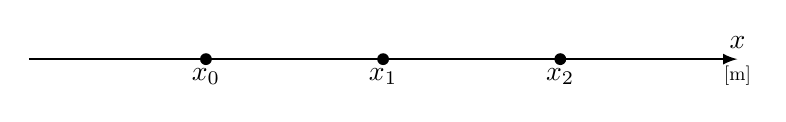
\begin{tikzpicture}[scale=1.5]
   \draw[->,thick,-latex] (-1.75,0) -- (4.25,0) node [anchor=north ,scale=0.7] {$[\text{m}]$}node [anchor=south ,scale=1] {$x $}; 
     \fill[black] (-0.25,0) circle (0.5mm) node [anchor=north ,scale=1] {$x_0$};
   \fill[black] (1.25,0) circle (0.5mm) node [anchor=north ,scale=1] {$x_1$};
    \fill[black] (2.75,0) circle (0.5mm) node [anchor=north ,scale=1] {$x_{2}$};
   
   \end{tikzpicture}
   $$
   A sum of values is known as a series.  Series may be represented using sigma notation.
$$x_0+x_1+x_2 \dots x_M=\sum_{i=0}^{M}x_i$$

\marginnote[-90pt]{$\braket{x}$ is the mean, or average value of a set.  $\sigma$ is the uncertainty or standard deviation.
$$\braket{x}=\frac{x_0+x_1+x_2 \dots}{N}$$
$$\braket{x^2}=\frac{x_0^2+x_1^2+x_2^2 \dots}{N}$$
$$\sigma^2= \braket{x^2}-\braket{x}^2$$
}
  
\section{Difference} 
The delta operator $\Delta$ indicates difference.  $\Delta x$ is a change in $x$ from $x=a$ to $x=b$.
$\Delta x = b-a$, or indexed $\Delta x_i = x_{i+1}-x_i$.
$$\{ \Delta x_i\}=\{x_1 -x_0,x_2-x_1,\dots ,x_N-x_{N-1}\}$$
 

\marginnote[-50pt]{For any sequence $x_i$ with $N$ elements we can generate a sequence $\Delta x_i$ of changes.  This is a mapping of one sequence to another.\\ \  \\
\texttt{
for (i=0,i<N-1,i=i+1)\\
\ \ \ \ \ dx[i]=x[i+1]-x[i]
	}\\ 
	\Large $$\{x_i\}\xrightarrow{\ \ \Delta \ \ }\{ \Delta x_i\}$$
}
$$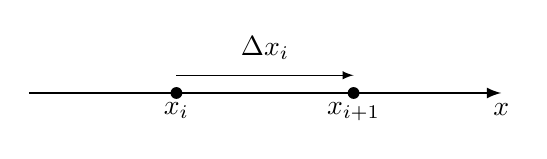
\begin{tikzpicture}[scale=1.5]
   \draw[->,thick,-latex] (0,0) -- (4,0) node [anchor=north ,scale=1] {$x$}; 
      \draw[->,-latex] (1.25,0.15) -- (2.75,0.15)  node [black,midway,above=0pt,yshift=2pt] { $\Delta x_i$}; 
   \fill[black] (1.25,0) circle (0.5mm) node [anchor=north ,scale=1] {$x_i$};
    \fill[black] (2.75,0) circle (0.5mm) node [anchor=north ,scale=1] {$x_{i+1}$};
   
   \end{tikzpicture}
   $$

\section{Accumulation}
Accumulation is the inverse of difference.  Rather than subtract successive terms we add them.  It is the summation of a sequence as a series.  The summation of $\Delta x_i$ returns us to the sequence $x_i$.
\marginnote[-25pt]{For any sequence $\Delta x_i$ of changes we can generate a sequence $x_i$ (up to a constant).  This is the reverse mapping.\\ \ \\ \ \\ \ \\
\texttt{for (i=0,i<N-1,i=i+1)\\
\ \ \ \ \ x[i+1]=x[i]+dx[i]
	}\\ \ \\
	\Large$$\{\Delta x_i\}\xrightarrow{\ \ \sum \ \ }\{  x_i\}$$
}

$$\sum_{n=0}^{i-1}\Delta x_n=x_i-x_0$$
$$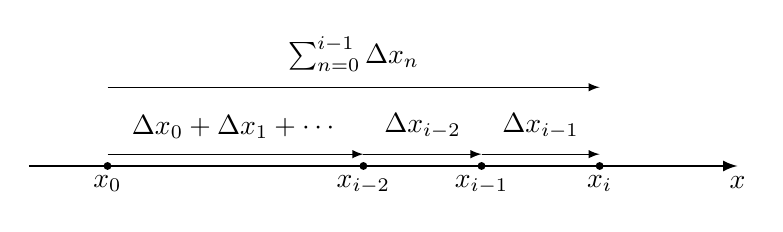
\begin{tikzpicture}[scale=1]
   \draw[->,thick,-latex] (-3,0) -- (6,0) node [anchor=north ,scale=1] {$x$}; 
      \draw[->,-latex] (-2,0.15) -- (1.25,0.15)  node [black,midway,above=0pt,yshift=2pt] { $\Delta x_{0}+\Delta x_{1}+\cdots$}; 
        \draw[->,-latex] (1.25,0.15) -- (2.75,0.15)  node [black,midway,above=0pt,yshift=2pt] { $\Delta x_{i-2}$}; 
          \draw[->,-latex] (2.75,0.15) -- (4.25,0.15)  node [black,midway,above=0pt,yshift=2pt] { $\Delta x_{i-1}$}; 
       \fill[black] (-2,0) circle (0.5mm) node [anchor=north ,scale=1] {$x_0$};
   \fill[black] (1.25,0) circle (0.5mm) node [anchor=north ,scale=1] {$x_{i-2}$};
    \fill[black] (2.75,0) circle (0.5mm) node [anchor=north ,scale=1] {$x_{i-1}$};
     \fill[black] (4.25,0) circle (0.5mm) node [anchor=north ,scale=1] {$x_{i}$};
     \draw[->,-latex] (-2,1) -- (4.25,1)  node [black,midway,above=0pt,yshift=2pt] { $\sum_{n=0}^{i-1}\Delta x_n$}; 

   
   \end{tikzpicture}
   $$

  
\section{Functions}
Given a sequence of discrete ordered pairs $\{x_i,y_i\}$ we can graph points on a 2-dimensional graph using two number lines.  We can model the relationship using a continuous function, $y=f(x)$.
\begin{figure}
$$
\begin{tikzpicture}
      [yscale=0.8, xscale=0.8,line cap=round,line join=round,x=2cm,y=2cm]%main layer

%main layer
%creating the ticks and xy-axis nodes
  \draw[-latex,color=black,thin] (-0.4,0) -- (2.8,0) node [anchor=north ,scale=1] {$x$};
   \draw[-latex,color=black,thin] (0,-0.4) -- (0,1.5)node [anchor=east ,scale=1] {$y$};
 \draw (0.5,1.2) node [anchor=west ,scale=1] {$\{x_i,y_i\}$};
%some function


 
\foreach \x in {-4,...,26}
                             \draw[fill] (\x*0.1,{1/2*(\x*.1) ^2-1/24*(\x*.1)^4+rand*0.1}) circle [radius=.5pt];

\begin{scope}[shift={(3.5,0)}]

  \draw[-latex,color=black,thin] (-0.4,0) -- (2.8,0) node [anchor=north ,scale=1] {$x$};
   \draw[-latex,color=black,thin] (0,-0.4) -- (0,1.5)node [anchor=east ,scale=1] {$y$};
    \draw (0.5,1.2) node [anchor=west ,scale=1] {$f(x)$};

%some function

 \draw[smooth,samples=100,domain=-0.4:2.6]
                             plot(\x,{1/2*(\x) ^2-1/24*(\x)^4});
 
\end{scope}

\end{tikzpicture}
$$

\caption{Ordered pairs $\{x_i,y_i\}$ and continuous function $f(x)$}
  \label{fig:function}
\end{figure}


\begin{figure}
$$
\begin{tikzpicture}
      [yscale=0.8, xscale=0.8,line cap=round,line join=round,x=2cm,y=2cm]%main layer

%main layer
%creating the ticks and xy-axis nodes
  \draw[-latex,color=black,thin] (-0.4,0) -- (2.8,0) node [anchor=north ,scale=1] {$x$};
   \draw[-latex,color=black,thin] (0,-0.4) -- (0,1.5)node [anchor=east ,scale=1] {$y$};
    \draw (0.6,1.2) node [anchor=west ,scale=1] {$\sin (x) $};
    \draw (0.6,-0.6) node [anchor=west ,scale=1] {$\cos (x) $};

%some function

 \draw[smooth,samples=100,domain=-0.4:2.6]
                             plot(\x,cos(90* \x));
                             
  \draw[smooth,samples=100,domain=-0.4:2.6]
                             plot(\x,sin(90* \x));
 
 
\begin{scope}[shift={(0,2.5)}]
%main layer
%creating the ticks and xy-axis nodes
  \draw[-latex,color=black,thin] (-0.4,0) -- (2.8,0) node [anchor=north ,scale=1] {$x$};
   \draw[-latex,color=black,thin] (0,-0.4) -- (0,1.5)node [anchor=east ,scale=1] {$y$};
    \draw (0.75,1.3) node [anchor=west ,scale=1] {$\sqrt{x}$};
    \draw (0.75,0.45) node [anchor=west ,scale=1] {$\nicefrac{1}{x}$};

%some function

 \draw[smooth,samples=100,domain=0.15:2.6]
                             plot(\x,0.2/\x);
                             
  \draw[smooth,samples=100,domain=0:2.6]
                             plot(\x,sqrt \x);
 \end{scope}
 
 
\begin{scope}[shift={(-3.5,2.5)}]
%main layer
%creating the ticks and xy-axis nodes
  \draw[-latex,color=black,thin] (-0.4,0) -- (2.8,0) node [anchor=north ,scale=1] {$x$};
   \draw[-latex,color=black,thin] (0,-0.4) -- (0,1.5)node [anchor=east ,scale=1] {$y$};
    \draw (0.75,1.2) node [anchor=west ,scale=1] {$mx+b$};
    \draw (0.6,0.2) node [anchor=west ,scale=1] {$ax^2+bx+c$};

%some function

 \draw[smooth,samples=100,domain=-0.4:2.6]
                             plot(\x,\x*.4+0.3);
                             
  \draw[smooth,samples=100,domain=-0.4:2.6]
                             plot(\x,\x*\x*0.33-.8*\x+.3);
 \end{scope}
 
 \begin{scope}[shift={(-3.5,0)}]
%main layer
%creating the ticks and xy-axis nodes
  \draw[-latex,color=black,thin] (-0.4,0) -- (2.8,0) node [anchor=north ,scale=1] {$x$};
   \draw[-latex,color=black,thin] (0,-0.4) -- (0,1.5)node [anchor=east ,scale=1] {$y$};
    \draw (0.75,1.2) node [anchor=west ,scale=1] {$e^x$};
    \draw (0.75,-0.6) node [anchor=west ,scale=1] {$\log(x) $};

%some function

 \draw[smooth,samples=100,domain=-0.4:2]
                             plot(\x,0.3*exp (\x*0.8) );
                             
  \draw[smooth,samples=100,domain=0.5:2.6]
                             plot(\x,ln \x);
 \end{scope}
 
\end{tikzpicture}
$$
\caption{Common functions}
  \label{fig:function}
\end{figure}
\begin{margintable}[-300pt]
\begin{center}
\footnotesize
\begin{tabular}{lllll}
\toprule
 Function              & Formula                                                                         \\
\midrule
  Linear   & $y=mx+b$       \\
  Quadratic  & $y=ax^2+bx+c$           \\
    Reciprocal    & $y=\frac{1}{x}$                        \\
    Power         & $y=x^n$                                                        \\
    Exponential        & $y=a^x$                              \\
    Logarithmic          & $y=\log_a b$          \\
     Sine         & $y=\sin x$                                                        \\
    Cosine       & $y=\cos x$                              \\
    Tangent        & $y=\tan x$          \\
  Arc sine         & $y=\sin^{-1} x$                                                        \\
    Arc cosine       & $y=\cos^{-1} x$                              \\
    Arc tangent        & $y=\tan^{-1} x$          \\
\bottomrule
\end{tabular}
\end{center}
  \caption{A list of common functions}
  \label{tab:font-sizes}
\end{margintable}

\subsection{Changing Functions}
\newthought{Changes in the value of a function} generate difference in $f(x)$.  There is a relationship between $\Delta f$ and $\Delta x$.
\begin{fullwidth}
\begin{figure}[h]
$$
\definecolor{darkgray}{rgb}{0.25,0.25,0.25}
\definecolor{lightgray}{rgb}{0.75,0.75,0.75}
%
\definecolor{darkgray}{rgb}{0.25,0.25,0.25}
\definecolor{lightgray}{rgb}{0.75,0.75,0.75}
%
\begin{tikzpicture}
      [yscale=1.3, xscale=3.3,line cap=round,line join=round,x=2cm,y=2cm,
     %using the 'spy' to magnify a part of the picture
     spy using outlines={rectangle,lens={scale=3}, size=4.5cm, connect spies},
     %using the decoration 'brace' (=a curly brace as path replacement)
     decoration={brace,amplitude=2pt}]%main layer

%main layer
%creating the ticks and xy-axis nodes
  \draw[-latex,color=black,thin] (-0.2,0) -- (1.4,0) node [anchor=north ,scale=1] {$x$};
   \draw[-latex,color=black,thin] (0,-0.2) -- (0,1.4)node [anchor=east ,scale=1] {$y$};
    \draw (1,1) node [anchor=west ,scale=1] {$f(x)$};
 
%some function

 \draw[smooth,samples=100,domain=-0.2:1.3]
                             plot(\x,{1/2*(\x*2) ^2-1/24*(\x*2)^4});
 
  \draw [darkgray,ultra thin] (0,0.1224)-- (0.25,0.1224);
  \draw [darkgray,ultra thin] (0,0.914)-- (0.75,0.914);
  \draw [darkgray,ultra thin] (0.25,0.1224)-- (0.25,0.0);
  \draw [darkgray,ultra thin] (0.75,0.914)-- (0.75,0);
%creating the curly braces with decorate
  \draw [decorate,color=black] (-0.01,0.1224) -- (-0.01,0.914) 
   node [midway,anchor=east,inner sep=2pt, outer sep=1pt]{\small$\Delta f$};
  \draw [decorate,color=black!80!black] (0.75,-0.02) -- (0.25,-0.02)
   node [midway,anchor=north,inner sep=1pt, outer sep=1pt]{\small$\Delta x$};
    \draw (0.75,-0.05)  node [anchor=north ,scale=0.75] {$b$};
     \draw (.25,-0.05) node [anchor=north ,scale=0.75] {$a$};
      \draw (0,0.1224)  node [anchor=east ,scale=0.75] {$f(a) \ $};
     \draw (0,0.914) node [anchor=east ,scale=0.75] {$f(b) \ $};
\end{tikzpicture}
$$

\caption{Difference on a continuous function $f(x)$}
  \label{fig:function-delta}
\end{figure}
\end{fullwidth}
\vspace{0.5cm}
\marginnote[0pt]{\textit{Difference is the object of a practical affirmation inseparable from essence and constitutive of existence.}\textbf{- Gilles Deleuze}}
$$\Delta f= f(b)-f(a)$$
$$\Delta f= f(a+\Delta x)-f(a)$$


\newpage

\subsection{Slope, Tangent Line \& Slope Function }
The \textbf{slope} is a ratio of difference between two points on the function graph.  The construction of the right triangle with sides $\Delta x$ and $\Delta y$ yields a tangent which is equivalent to the slope.  In the limit of small $\Delta$ we call the slope a \textbf{tangent line}.
\begin{figure}[ht]
$$\definecolor{darkgray}{rgb}{0.25,0.25,0.25}
\definecolor{lightgray}{rgb}{0.75,0.75,0.75}
%
\definecolor{darkgray}{rgb}{0.25,0.25,0.25}
\definecolor{lightgray}{rgb}{0.75,0.75,0.75}
%
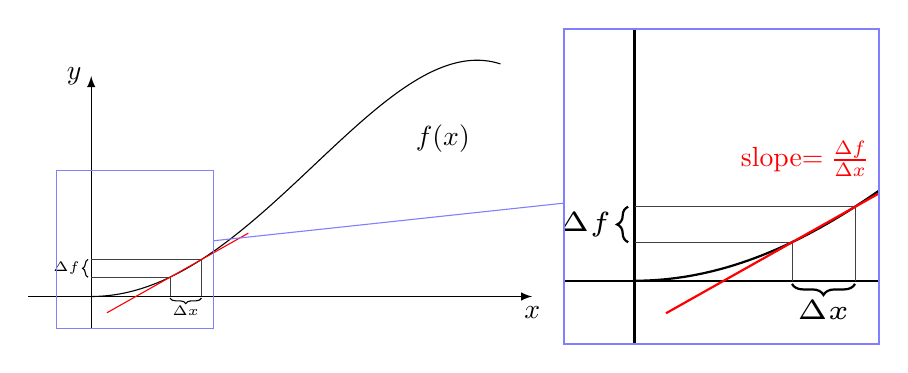
\begin{tikzpicture}
   [xscale=2,line cap=round,line join=round,x=2cm,y=2cm,
     %using the 'spy' to magnify a part of the picture
     spy using outlines={rectangle,lens={scale=2}, size=4cm, connect spies},
     %using the decoration 'brace' (=a curly brace as path replacement)
     decoration={brace,amplitude=2pt}]%main layer
%creating the ticks and xy-axis nodes
  \draw[-latex,color=black,thin] (-0.2,0) -- (1.4,0) node [anchor=north ,scale=1] {$x$};
   \draw[-latex,color=black,thin] (0,-0.2) -- (0,1.4)node [anchor=east ,scale=1] {$y$};
    \draw (1,1) node [anchor=west ,scale=1] {$f(x)$};
 
%some function

 \draw[smooth,samples=100,domain=0.0:1.3]
                             plot(\x,{1/2*(\x*2) ^2-1/24*(\x*2)^4});
 
  \draw [darkgray,ultra thin] (0,0.1224)-- (0.25,0.1224);
  \draw [darkgray,ultra thin] (0,0.235)-- (0.35,0.235);
  \draw [darkgray,ultra thin] (0.25,0.1224)-- (0.25,0.0);
  \draw [darkgray,ultra thin] (0.35,0.235)-- (0.35,0);
%creating the curly braces with decorate
  \draw [decorate,color=black] (-0.01,0.1224) -- (-0.01,0.235)
   node [midway,anchor=east,inner sep=2pt, outer sep=1pt]{\tiny$\Delta f $};
  \draw [decorate,color=black!80!black] (0.35,-0.01)--(0.25,-0.01)
   node [midway,anchor=north,inner sep=1pt, outer sep=2pt]{\tiny$ \Delta x$};
   
    \draw[smooth,color=red, samples=100,domain=0.05:0.5]
                             plot(\x,{((0.235-0.1224)/0.1)*(\x-0.25)+0.122});

   
   \spy [blue!50] on (0.275,0.3)
             in node [left] at (2.5,0.7);
             
                \draw (2.5,0.7) node [anchor=south east,color=red ,scale=1] {slope$=\frac{\Delta f}{\Delta x}$};
\end{tikzpicture}
$$\\ \ \\ 
$$\definecolor{darkgray}{rgb}{0.25,0.25,0.25}
\definecolor{lightgray}{rgb}{0.75,0.75,0.75}
%
\definecolor{darkgray}{rgb}{0.25,0.25,0.25}
\definecolor{lightgray}{rgb}{0.75,0.75,0.75}
%
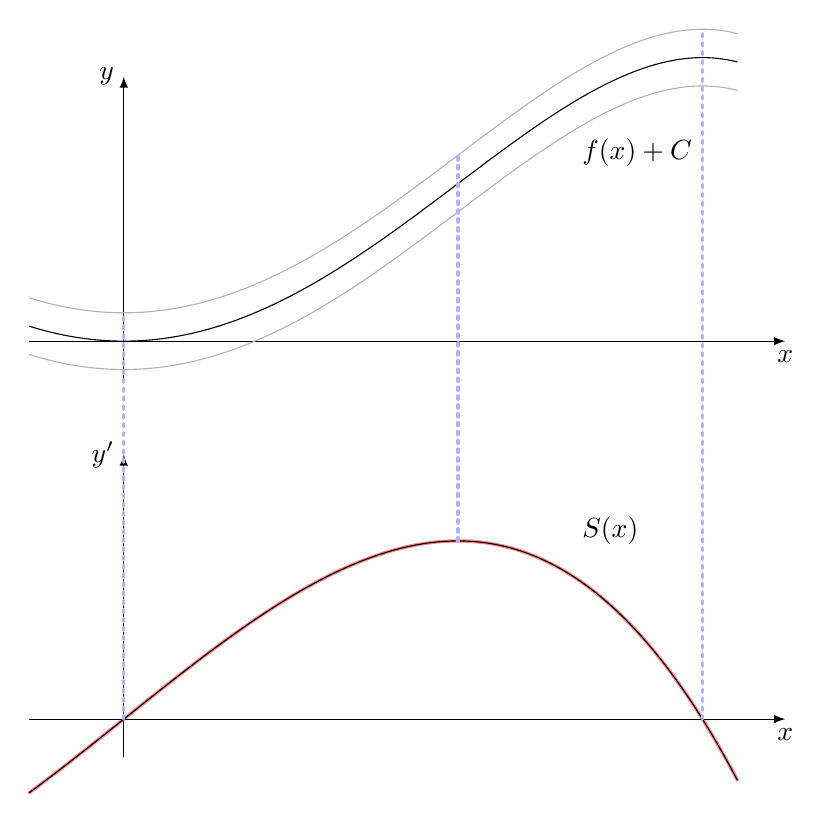
\begin{tikzpicture}
      [line cap=round,line join=round,x=2cm,y=2cm, yscale=1.2, xscale=3]
   

%main layer
%creating the ticks and xy-axis nodes
  \draw[-latex,color=black,thin] (-0.2,0) -- (1.4,0) node [anchor=north ,scale=1] {$x$};
   \draw[-latex,color=black,thin] (0,-0.2) -- (0,1.4)node [anchor=east ,scale=1] {$y$};
    \draw (0.95,1) node [anchor=west ,scale=1] {$f(x)+C$};
 
%some function

 \draw[smooth,samples=100,domain=-0.2:1.3] plot(\x,{1/2*(\x*2) ^2-1/24*(\x*2)^4});
  \draw[smooth,samples=100,domain=-0.2:1.3,color=black!30] plot(\x,{1/2*(\x*2) ^2-1/24*(\x*2)^4-0.15});
   \draw[smooth,samples=100,domain=-0.2:1.3,color=black!30] plot(\x,{1/2*(\x*2) ^2-1/24*(\x*2)^4+0.15});
 
 \begin{scope}[shift={(0,-2)}]
 	\draw[smooth,samples=100,domain=-0.2:1.3,color=red!50, very thick] plot(\x,{(\x*2)-1/6*(\x*2)^3});            
	\draw[smooth,samples=100,domain=-0.2:1.3,thin] plot(\x,{(\x*2)-1/6*(\x*2)^3});                   
	       
	\draw[-latex,color=black,thin] (-0.2,0) -- (1.4,0) node [anchor=north ,scale=1] {$x$};
	\draw[-latex,color=black,thin] (0,-0.2) -- (0,1.4)node [anchor=east ,scale=1] {$y'$};
	\draw (0.95,1) node [anchor=west ,scale=1] {$S(x)$};
 \end{scope}
 
 \draw[dotted,color=blue!30, very thick] (1.225,-2) -- (1.225,1.65);
 \draw[dotted,color=blue!30, very thick] (0,-2) -- (0,0.15);
 \draw[dotted,color=blue!30,very thick] (0.707,-1.057) -- (0.707,0.983);
 
\end{tikzpicture}$$

\caption{Tangent lines and the slope function S(x) for a function $f(x)$}
  \label{fig:function-delta}
\end{figure}

\marginnote[-260pt]{
This specific function $f(x)$ is 
$$y=x^2-\frac{x^4}{12}$$}

\marginnote[-450pt]{
\Large $$\text{slope}=\frac{\text{rise}}{\text{run}}=\frac{\Delta f}{\Delta x}$$}

\marginnote[-130pt]{
$$S(x)=\text{slope of tangent line}=\mathop {\lim }\limits_{\Delta x \to 0} {\frac{\Delta f}{\Delta x}}$$\\ \ \\
This specific slope function $S(x)$ is \\ \ \\
$$y=2x-\frac{x^3}{3}$$
}

\noindent The \textbf{slope function} $S(x)$ represents the slope of the tangent line at any point $x$.


\newpage


\subsection{Accumulation of a Slope Function}
Over some range $\Delta x$ the area beneath the slope function represents some accumulation of $S(x)$.  The total area represents $\Delta f$  over the range $\Delta x$.
\begin{figure}[ht]
$$\definecolor{darkgray}{rgb}{0.25,0.25,0.25}
\definecolor{lightgray}{rgb}{0.75,0.75,0.75}
%
\definecolor{darkgray}{rgb}{0.25,0.25,0.25}
\definecolor{lightgray}{rgb}{0.75,0.75,0.75}
%
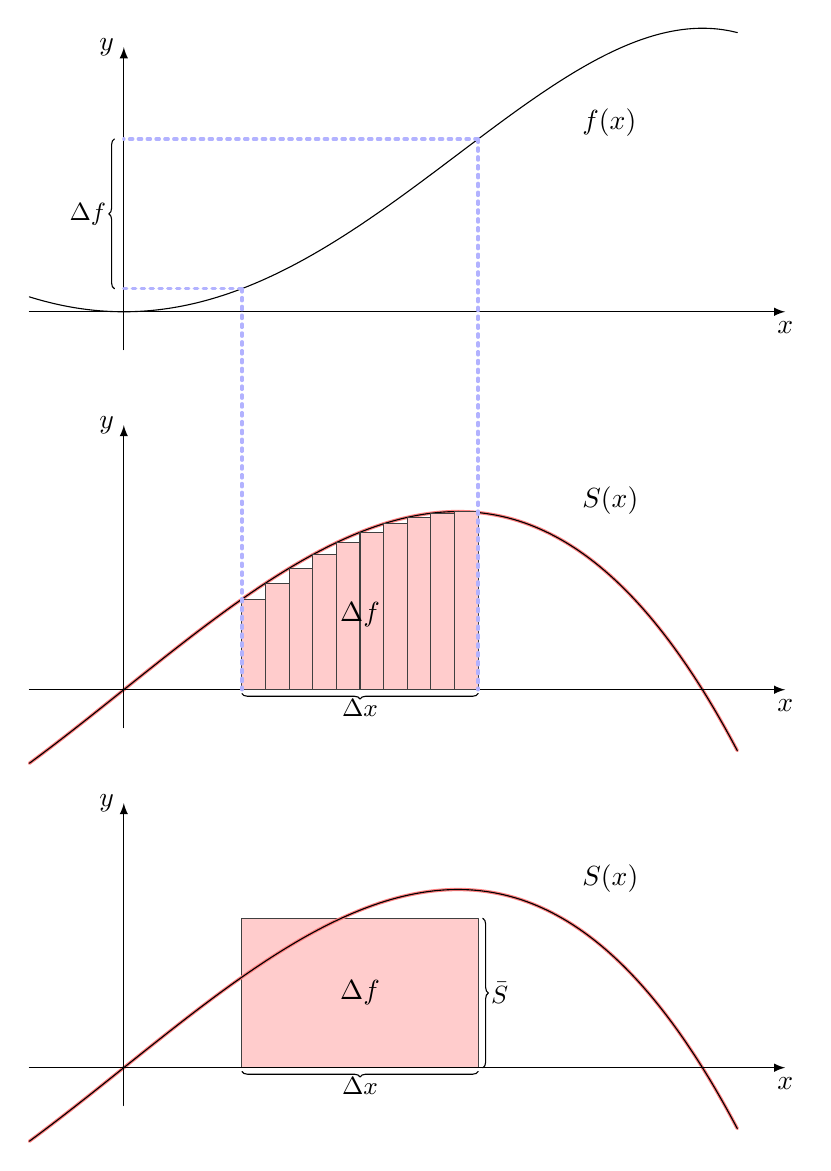
\begin{tikzpicture}
      [line cap=round,decoration={brace,amplitude=2pt},line join=round,x=2cm,y=2cm, yscale=1.2, xscale=3]
   

%main layer
%creating the ticks and xy-axis nodes
  \draw[-latex,color=black,thin] (-0.2,0) -- (1.4,0) node [anchor=north ,scale=1] {$x$};
   \draw[-latex,color=black,thin] (0,-0.2) -- (0,1.4)node [anchor=east ,scale=1] {$y$};
    \draw (0.95,1) node [anchor=west ,scale=1] {$f(x)$};
 
%some function

 \draw[smooth,samples=100,domain=-0.2:1.3] plot(\x,{1/2*(\x*2) ^2-1/24*(\x*2)^4});
 
 
 \begin{scope}[shift={(0,-2)}]
 	\draw[smooth,samples=100,domain=-0.2:1.3,color=red!50, very thick] plot(\x,{(\x*2)-1/6*(\x*2)^3});            
	\draw[smooth,samples=100,domain=-0.2:1.3,thin] plot(\x,{(\x*2)-1/6*(\x*2)^3});                   
	       
	\draw[-latex,color=black,thin] (-0.2,0) -- (1.4,0) node [anchor=north ,scale=1] {$x$};
	\draw[-latex,color=black,thin] (0,-0.2) -- (0,1.4)node [anchor=east ,scale=1] {$y$};
	\draw (0.95,1) node [anchor=west ,scale=1] {$S(x)$};
	
	 \foreach \x in {0.25,0.3,0.35,0.4,0.45,0.5,0.55,0.6,0.65,0.7}
   \fill[color=red!20,thin] (\x,0) -- (\x,{(\x*2)-1/6*(\x*2)^3}) -- (\x+0.05,{(\x*2)-1/6*(\x*2)^3}) -- (\x+0.05,0) -- cycle;
   \foreach \x in {0.25,0.3,0.35,0.4,0.45,0.5,0.55,0.6,0.65,0.7}
   \draw[color=darkgray,thin] (\x,0) -- (\x,{(\x*2)-1/6*(\x*2)^3}) -- (\x+0.05,{(\x*2)-1/6*(\x*2)^3}) -- (\x+0.05,0) -- cycle;

  \draw [decorate,color=black!80!black] (0.75,-0.02) -- (0.25,-0.02)
   node [midway,anchor=north,inner sep=1pt, outer sep=1pt]{\small$\Delta x$};
    \draw (0.5,0.4)
   node [anchor=center,scale=1]{$\Delta f$};
 \end{scope}
 
 \draw[dotted,color=blue!30, very thick] (0.25,0.1224) -- (0,0.1224);
 \draw[dotted,color=blue!30, very thick] (0.75,0.914) -- (0,0.914);
 \draw[dotted,color=blue!30, very thick] (0.25,0.1224) -- (0.25,-2);
 \draw[dotted,color=blue!30, very thick] (0.75,0.914) -- (0.75,-2);

 
   \draw [decorate,color=black] (-0.02,0.1224) -- (-0.02,0.914) 
   node [midway,anchor=east,inner sep=2pt, outer sep=1pt]{\small$\Delta f$};
  
   \begin{scope}[shift={(0,-4)}]
   \fill[color=red!20,thin] (0.25,0) -- (0.25,0.79) -- (0.75,0.79) -- (0.75,0) -- cycle;
   \draw[color=darkgray,thin] (0.25,0) -- (0.25,0.79) -- (0.75,0.79) -- (0.75,0) -- cycle;
 	\draw[smooth,samples=100,domain=-0.2:1.3,color=red!50, very thick] plot(\x,{(\x*2)-1/6*(\x*2)^3});            
	\draw[smooth,samples=100,domain=-0.2:1.3,thin] plot(\x,{(\x*2)-1/6*(\x*2)^3});                   
	       
	\draw[-latex,color=black,thin] (-0.2,0) -- (1.4,0) node [anchor=north ,scale=1] {$x$};
	\draw[-latex,color=black,thin] (0,-0.2) -- (0,1.4)node [anchor=east ,scale=1] {$y$};
	\draw (0.95,1) node [anchor=west ,scale=1] {$S(x)$};

  \draw [decorate,color=black!80!black] (0.75,-0.02) -- (0.25,-0.02)
   node [midway,anchor=north,inner sep=1pt, outer sep=1pt]{\small$\Delta x$};
   
     \draw [decorate,color=black] (0.76,0.79) -- (0.76,0) 
   node [midway,anchor=west,inner sep=2pt, outer sep=1pt]{\small$\bar{S}$};
   
   \draw (0.5,0.4) node [anchor=center ,scale=1] {$\small\Delta f$};
   
 \end{scope}
  
\end{tikzpicture}$$
\caption{Area underneath a slope function $S(x)$}
  \label{fig:functiona-delta}
\end{figure}

\marginnote[-140pt]{
 \Large $$\bar{S}=\frac{\Delta f}{\Delta x}$$\\
 
 \Large  $$\Delta f=\bar{S}\cdot {\Delta x}$$
   }
   \noindent If this area representing $\Delta f$ is represented as a rectangle with base $\Delta x$ the height of the rectangle is the average value $\bar{S}$.
\newpage


\section{Scalars and Vectors}
A \textbf{scalar} is a one-dimensional physical quantity, i.e. one that can be described by a single real number (signed, with units).  It is a physical quantity that only has magnitude but no direction.  A \textbf{vector} is a geometric object that has magnitude (or length) and direction and can be added to other vectors according to vector algebra.  A vector can be represented by a set of scalars.  

$\overrightarrow{x}$ is a vector.  $x$ is the magnitude (or length) of the vector $\overrightarrow{x}$.  The vector $\hat{x}$ is the directional vector of $\overrightarrow{x}$.  It has a magnitude of 1 rand points in the same direction as $\overrightarrow{x}$.  
\marginnote[-100pt]{ \Large
$$\overrightarrow{x}=x\hat{x}$$\\ \ \\
$$|\overrightarrow{x}|=x$$\\ \ \\
$$\hat{x}=\frac{\overrightarrow{x}}{x}$$\\ \ \\
$$|\hat{x}|=1$$
}
$$
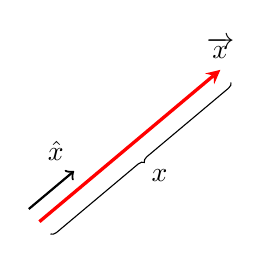
\begin{tikzpicture}[scale=3,decoration={brace,amplitude=2pt}]



%draw a vector from origin to point (P) 
\begin{scope}[rotate=40]
\draw[-stealth,very thick,color=red] (0,0) -- (1,0) node[anchor=south,color=black]{$\overrightarrow{x}$};
  \draw[->,thick,color=black] (0,0.07) -- (0.25,0.07) node[anchor=south east,color=black]{$\hat{x}$};
   \draw [decorate,color=black] (1,-0.07) -- (0,-0.07) 
   node [midway,anchor=north west,inner sep=2pt, outer sep=2pt]{$x$};
   \end{scope}



\end{tikzpicture}
$$

\section{Spatial Coordinate Systems}
\subsection{2D Cartesian $(x,y)$}


In two dimensions we use the vector representation $\overrightarrow{r}$ with components $x$ and $y$.  This can be represented as a column vector or using the unit vectors $\hat{x}$ and $\hat{y}$.  The magnitude of the vector $\overrightarrow{r}$ is $r$.  We can calculate $r$ given the $x$ and $y$ components using the Pythagorean theorem.

$x$ (or $r_x$) and $y$ (or $r_y$) are called orthogonal components of $\overrightarrow{r}$ meaning $\hat{x}$ and $\hat{y}$ do not overlap at all, namely they meet at 90 degrees.

\marginnote[-20pt]{\Large
$$\overrightarrow{r}=x\hat{x}+y\hat{y}$$\\ \ \\
$$ \overrightarrow{r}=\left(\begin{array}{c} x \\ y \end{array}\right)$$\\ \ \\
$$r=\sqrt{x^2+y^2}$$\\ \ \\
$$\hat{r}=\left(\begin{array}{c} \nicefrac{x}{\sqrt{x^2+y^2}} \\ \nicefrac{y}{\sqrt{x^2+y^2}} \end{array}\right)$$
}
\vspace{1cm}
$$
\begin{tikzpicture}[scale=1.5]


\draw[thick,->] (0,0,0) -- (3,0,0) node[anchor=north east]{$x$};
\draw[thick,->] (0,0,0) -- (0,3,0) node[anchor=north west]{$y$};


%draw a vector from origin to point (P) 
\draw[-stealth,very thick,color=red] (0,0) -- (1,2) node[anchor=south west,color=black]{$\overrightarrow{r}$};


%draw projection on xy plane, and a connecting line
\draw[dashed, color=red] (1,0) -- (1,2) node[midway,anchor=west ,scale=1,color=black] {$r_y$};
\draw[dashed, color=red] (0,2) -- (1,2) node[midway,anchor=south ,scale=1,color=black] {$r_x$};
\end{tikzpicture}
$$
\newpage
\subsection{Polar Coordinates $(r,\theta)$ }
In polar coordinates we parameterize the vector $\overrightarrow{r}$ in terms of its length and direction rather than in terms of the $x$ and $y$ components.  The length of the vector $\overrightarrow{r}$ is $r$ and the direction is expressed in terms of $\theta$.  The vector $\overrightarrow{r}$ makes an angle $\theta$ with the unit vector $\hat{x}$.  We can easily convert between polar coordinates $(r,\theta)$ and 2-D cartesian coordinates $(x,y)$. 

\marginnote[-80pt]{\Large

$$\overrightarrow{r}=r\hat{r}$$\\ \ \\
$$r=\sqrt{x^2+y^2}$$\\ \ \\
$$\theta=\tan^{-1}\left(\frac{y}{x}\right)$$\\ \ \\
$$x=r\cos\theta$$\\ \ \\
$$y=r\sin\theta$$\\ \ \\
$$\hat{r}=\left(\begin{array}{c} \cos \theta \\ \sin \theta \end{array}\right)$$\\ \ \\ \ \\

\footnotesize
In mathematics, the polar coordinate system is a two-dimensional coordinate system in which each point on a plane is determined by a distance from a reference point and an angle from a reference direction.\\ 

The reference point (analogous to the origin of a Cartesian system) is called the pole, and the ray from the pole in the reference direction is the polar axis. The distance from the pole is called the radial coordinate or radius, and the angle is the angular coordinate, polar angle, or azimuth.\\ 

The concepts of angle and radius were already used by ancient peoples of the 1st millennium BC. The Greek astronomer and astrologer Hipparchus (190-120 BC) created a table of chord functions giving the length of the chord for each angle, and there are references to his using polar coordinates in establishing stellar positions. In On Spirals, Archimedes describes the Archimedean spiral, a function whose radius depends on the angle. The Greek work, however, did not extend to a full coordinate system.}

\vspace{1cm}
$$
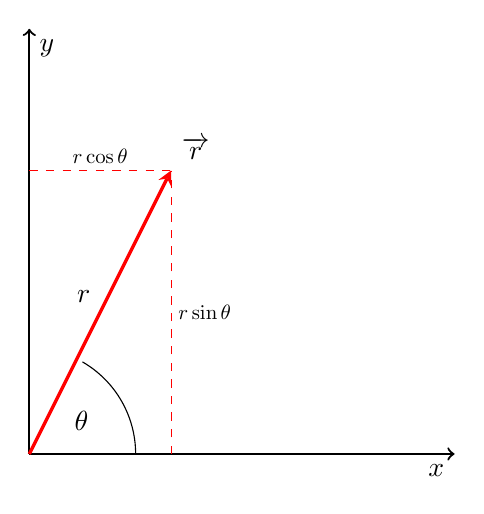
\begin{tikzpicture}[scale=1.8]


\draw[thick,->] (0,0,0) -- (3,0,0) node[anchor=north east]{$x$};
\draw[thick,->] (0,0,0) -- (0,3,0) node[anchor=north west]{$y$};


%draw a vector from origin to point (P) 
\draw[-stealth,very thick,color=red] (0,0) -- (1,2) node[anchor=south west,color=black]{$\overrightarrow{r}$};
\draw[color=red] (0,0) -- (0.5,1) node[anchor=south east ,color=black]{$r$};
\draw[dashed, color=red] (1,0) -- (1,2) node[midway,anchor=west ,scale=0.75,color=black] {$r\sin \theta$};
\draw[dashed, color=red] (0,2) -- (1,2) node[midway,anchor=south ,scale=0.75,color=black] {$r \cos \theta$};


%draw projection on xy plane, and a connecting line
\draw (0.75,0) arc (0:60:0.75) ;
\draw (0.25,0.1) node [anchor=south west,color=black]{$\theta$};
\end{tikzpicture}
$$
\vspace{1cm}
$$
  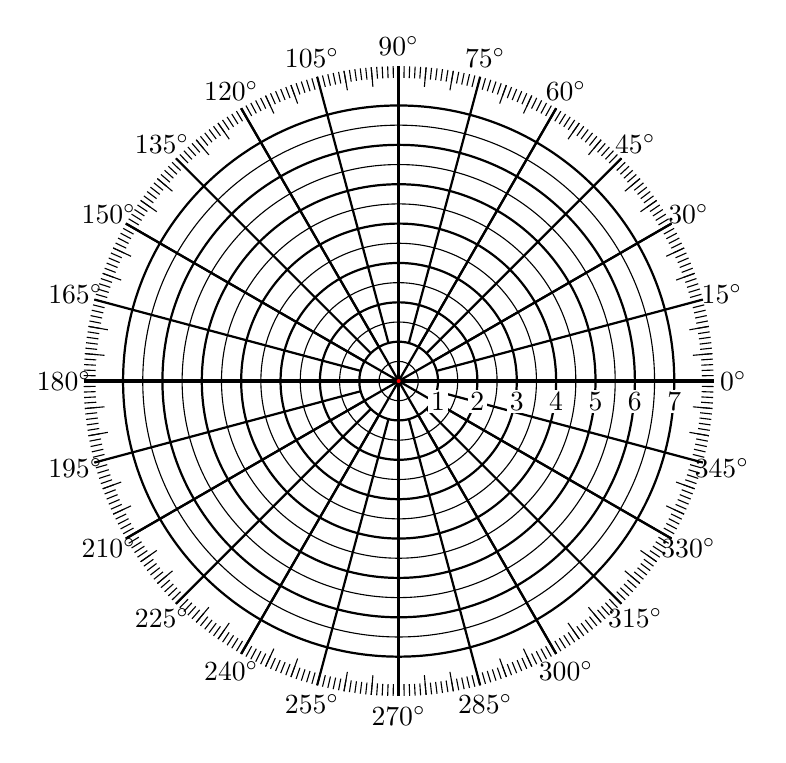
\begin{tikzpicture} [yscale=0.5, xscale=0.5]
    %Circles 
    \foreach \r in {1, 2,...,7}
      \draw[ thick] (0,0) circle (\r);    
    \foreach \r in {0.5, 1.5,...,7}
      \draw[thin] (0,0) circle (\r);
    %1� Rays
    \foreach \a in {0, 1,...,359}
      \draw[] (\a:7.7) -- (\a:8);
    %5� Rays
    \foreach \a in {0, 5,...,359}
      \draw[] (\a:7.5) -- (\a:8);      
    %15� Rays
    \foreach \a in {0, 15,...,359}
      \draw[thick] (\a:1) -- (\a:8); 
    %30� Rays
    \foreach \a in {0, 30,...,359}
      \draw[thick] (0, 0) -- (\a:8);
    %Radius labels (background filled white)
    \foreach \r in {1, 2,...,7}
      \draw (\r,0) node[inner sep=1pt,below=3pt,rectangle,fill=white] {$\r$};
    %Main rays
    \foreach \a in {0, 90,...,359}
      \draw[very thick] (0, 0) -- (\a:8);
    %Angle labels  
    \foreach \a in {0, 15,...,359}
      \draw (\a: 8.5) node {$\a^\circ$};
    %Central point
    \draw[fill=red] (0,0) circle(0.7mm);
  \end{tikzpicture}
$$

\newpage

\subsection{3D Cartesian $(x,y,z)$}
\marginnote[0pt]{
In three dimensions a vector can be described by three orthogonal components $(x,y,z)$.  It is the 3D cartesian coordinate system.  These form a right handed coordinate system so that if you look at the standard $(x,y)$ plane the z-axis comes straight out of the page.  The magnitude of $\overrightarrow{\scriptr}$ is determined using the Pythagorean Theorem (in 3D).\\
$$\scriptr=\sqrt{x^2+y^2+z^2}$$\\



The concept of Cartesian coordinates generalizes to allow axes that are not perpendicular to each other, and/or different units along each axis. In that case, each coordinate is obtained by projecting the point onto one axis along a direction that is parallel to the other axis (or, in general, to the hyperplane defined by all the other axes). In such an oblique coordinate system the computations of distances and angles must be modified from that in standard Cartesian systems, and many standard formulas (such as the Pythagorean formula for the distance) do not hold.\\ \ \\

We use the $\overrightarrow{\scriptr}$ to notate the vector in 3D and reserve $\overrightarrow{r}$ to represent the component in the xy-plane.  In cylindrical coordinates the vector $\overrightarrow{\scriptr}$ is represented using polar coordinates for  $\overrightarrow{r}$ and an orthogonal z-component.  Converting between cylindrical and 3D cartesian coordinates is identical to the polar and 2D cartesian conversion.}
\vspace{1cm}
$$\overrightarrow{\scriptr}=\overrightarrow{x}+\overrightarrow{y}+\overrightarrow{z}=x\hat{x}+y\hat{y}+z\hat{z}=\scriptr_x\hat{x}+\scriptr_y\hat{y}+\scriptr_z\hat{z}$$
$$ \overrightarrow{\scriptr}=\left(\begin{array}{c} x \\ y \\ z\end{array}\right)=\left(\begin{array}{c} \scriptr_x \\ \scriptr_y \\ \scriptr_z\end{array}\right)$$

\tdplotsetmaincoords{60}{110}
\begin{tikzpicture}[scale=1.2,tdplot_main_coords]
\coordinate (O) at (0,0,0);
\coordinate (P) at (1,2,3);

\draw[thick,->] (0,0,0) -- (4,0,0) node[anchor=north east]{$x$};
\draw[thick,->] (0,0,0) -- (0,4,0) node[anchor=north west]{$y$};
\draw[thick,->] (0,0,0) -- (0,0,4) node[anchor=south]{$z$};

%draw a vector from origin to point (P) 
\draw[-stealth,color=red] (O) -- (P) node[anchor=south,color=black]{$\overrightarrow{\scriptr}$};


%draw projection on xy plane, and a connecting line
\draw[dashed, color=red] (1,0,0) -- (1,2,0);
\draw[dashed, color=red] (0,2,0) -- (1,2,0);
\draw[dashed, color=red] (1,2,3) -- (1,2,0);

\draw (0.5,2,0) node [anchor=west ,scale=1] {$\scriptr_x$};
\draw (1,1,0) node [anchor=north ,scale=1] {$\scriptr_y$};
\draw (1,2,1.5) node [anchor=west ,scale=1] {$\scriptr_z$};

%draw the angle \phi, and label it
%syntax: \tdplotdrawarc[coordinate frame, draw options]{center point}{r}{angle}{label options}{label}
%\tdplotdrawarc{(O)}{0.2}{0}{\phivec}{anchor=north}{$\phi$}


%set the rotated coordinate system so the x'-y' plane lies within the
%"theta plane" of the main coordinate system
%syntax: \tdplotsetthetaplanecoords{\phi}
%\tdplotsetthetaplanecoords{\phivec}

%draw theta arc and label, using rotated coordinate system
%\tdplotdrawarc[tdplot_rotated_coords]{(0,0,0)}{0.5}{0}{\thetavec}{anchor=south west}{$\theta$}

\end{tikzpicture}

\subsection{Cylindrical $(r,\theta,z)$}
$$\overrightarrow{\scriptr}=\overrightarrow{r}+\overrightarrow{z}=r\hat{r}+z\hat{z}=\scriptr_r\hat{r}+\scriptr_z\hat{z}$$






\tdplotsetmaincoords{60}{110}
\begin{tikzpicture}[scale=1.2,tdplot_main_coords]
\coordinate (O) at (0,0,0);
\coordinate (P) at (1,2,3);

\draw[thick,->] (0,0,0) -- (4,0,0) node[anchor=north east]{$x$};
\draw[thick,->] (0,0,0) -- (0,4,0) node[anchor=north west]{$y$};
\draw[thick,->] (0,0,0) -- (0,0,4) node[anchor=south]{$z$};

%draw a vector from origin to point (P) 
\draw[-stealth,thick,color=red] (O) -- (P) node[anchor=south,color=black]{$\overrightarrow{\scriptr}$};


%draw projection on xy plane, and a connecting line

\draw[dashed, color=red] (0,0,0) -- (1,2,0);
\draw[dashed, color=red] (1,2,3) -- (1,2,0);


\draw (0.5,1,0) node [anchor=north ,scale=1] {$\scriptr_r$};
\draw (1,2,1.5) node [anchor=west ,scale=1] {$\scriptr_z$};

%draw the angle \phi, and label it
%syntax: \tdplotdrawarc[coordinate frame, draw options]{center point}{r}{angle}{label options}{label}
\tdplotdrawarc{(O)}{0.8}{0}{60}{anchor=north}{$\theta$}


%set the rotated coordinate system so the x'-y' plane lies within the
%"theta plane" of the main coordinate system
%syntax: \tdplotsetthetaplanecoords{\phi}
%\tdplotsetthetaplanecoords{\phivec}

%draw theta arc and label, using rotated coordinate system
%\tdplotdrawarc[tdplot_rotated_coords]{(0,0,0)}{0.5}{0}{\thetavec}{anchor=south west}{$\theta$}

\end{tikzpicture}
\hspace{1cm}
\tdplotsetmaincoords{60}{110}
\begin{tikzpicture}[scale=1,tdplot_main_coords]
\coordinate (O) at (0,0,0);
\coordinate (P) at (1,2,0);

\draw[thick,->] (0,0,0) -- (4,0,0) node[anchor=north east]{$x$};
\draw[thick,->] (0,0,0) -- (0,4,0) node[anchor=north west]{$y$};
\draw[thick,->] (0,0,0) -- (0,0,4) node[anchor=south]{$z$};

%draw a vector from origin to point (P) 
\draw[-stealth,color=red] (O) -- (P) node[anchor=north,color=black]{$\overrightarrow{r}$};


%draw projection on xy plane, and a connecting line


%draw the angle \phi, and label it
%syntax: \tdplotdrawarc[coordinate frame, draw options]{center point}{r}{angle}{label options}{label}
\tdplotdrawarc{(O)}{0.8}{0}{60}{anchor=north}{$\theta$}


%set the rotated coordinate system so the x'-y' plane lies within the
%"theta plane" of the main coordinate system
%syntax: \tdplotsetthetaplanecoords{\phi}
%\tdplotsetthetaplanecoords{\phivec}

%draw theta arc and label, using rotated coordinate system
%\tdplotdrawarc[tdplot_rotated_coords]{(0,0,0)}{0.5}{0}{\thetavec}{anchor=south west}{$\theta$}

\end{tikzpicture}
\newpage
\subsection{Spherical $(\scriptr,\theta,\phi)$}
\marginnote[0pt]{In a spherical coordinate system we represent the 3D vector $\overrightarrow{\scriptr}$ in terms of its magnitude (length) $\scriptr$, azimuthal angle $\theta$ and polar angle $\phi$.  The conversion between 3D cartesian or cylindrical coordinates and spherical coordinates are given.\\ \ \\ \
$$\hat{\scriptr}=\left(\begin{array}{c}  \sin \phi\ \cos\theta \\  \sin \phi\ \sin\theta \\ \cos \phi  \end{array}\right)$$ \\ \ \\ \ \\
A spherical coordinate system is a coordinate system for three-dimensional space where the position of a point is specified by three numbers: the radial distance of that point from a fixed origin, its polar angle measured from a fixed zenith direction, and the azimuth angle of its orthogonal projection on a reference plane that passes through the origin and is orthogonal to the zenith, measured from a fixed reference direction on that plane.\\ \ \\

The radial distance is also called the radius or radial coordinate. The polar angle may be called co-latitude, zenith angle, normal angle, or inclination angle.\\ \ \\

The mathematics used to describe electron distributions around atoms uses spherical coordinates.  The symmetry features of this mathematics gives rise to the structure of the periodic table.
}



\vspace{1cm}
$$\overrightarrow{\scriptr}=\scriptr \ \hat{\scriptr}$$
\vspace{1cm}
$$\scriptr=\sqrt{x^2+y^2+z^2}$$
$$\theta=\tan^{-1}\left(\frac{y}{x}\right)$$
$$\phi=\tan^{-1}\left(\frac{r}{z}\right)$$


\tdplotsetmaincoords{60}{110}

%define polar coordinates for some vector
%TODO: look into using 3d spherical coordinate system
\pgfmathsetmacro{\rvec}{.8}
\pgfmathsetmacro{\thetavec}{30}
\pgfmathsetmacro{\phivec}{60}

%start tikz picture, and use the tdplot_main_coords style to implement the display 
%coordinate transformation provided by 3dplot
\begin{tikzpicture}[scale=5,tdplot_main_coords]

%set up some coordinates 
%-----------------------
\coordinate (O) at (0,0,0);

%determine a coordinate (P) using (r,\theta,\phi) coordinates.  This command
%also determines (Pxy), (Pxz), and (Pyz): the xy-, xz-, and yz-projections
%of the point (P).
%syntax: \tdplotsetcoord{Coordinate name without parentheses}{r}{\theta}{\phi}
\tdplotsetcoord{P}{\rvec}{\thetavec}{\phivec}

%draw figure contents
%--------------------

%draw the main coordinate system axes
\draw[thick,->] (0,0,0) -- (1,0,0) node[anchor=north east]{$x$};
\draw[thick,->] (0,0,0) -- (0,1,0) node[anchor=north west]{$y$};
\draw[thick,->] (0,0,0) -- (0,0,1) node[anchor=south]{$z$};

%draw a vector from origin to point (P) 
\draw[-stealth,color=red] (O) -- (P) node[anchor=south,color=black]{$\overrightarrow{\scriptr}$};
\draw[color=red] (O) -- (P) node[midway,anchor=north west,color=black]{$\scriptr$};

%draw projection on xy plane, and a connecting line
\draw[dashed,-stealth, color=red] (O) -- (Pxy);
%\draw[dashed, color=red] (P) -- (Pxy);

%draw the angle \phi, and label it
%syntax: \tdplotdrawarc[coordinate frame, draw options]{center point}{r}{angle}{label options}{label}
\tdplotdrawarc{(O)}{0.2}{0}{\phivec}{anchor=north}{$\theta$}


%set the rotated coordinate system so the x'-y' plane lies within the
%"theta plane" of the main coordinate system
%syntax: \tdplotsetthetaplanecoords{\phi}
\tdplotsetthetaplanecoords{\phivec}

%draw theta arc and label, using rotated coordinate system
\tdplotdrawarc[tdplot_rotated_coords]{(0,0,0)}{0.5}{0}{\thetavec}{anchor=south west}{$\phi$}

\end{tikzpicture}


\vspace{1cm}

$$r=\scriptr \ \sin \phi $$
$$z=\scriptr \ \cos \phi $$
$$x=\scriptr\  \sin \phi\ \cos\theta$$
$$y=\scriptr\  \sin \phi\ \sin\theta$$
\begin{marginfigure}%
  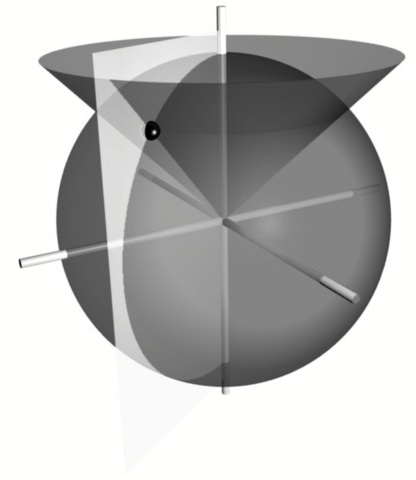
\includegraphics[width=\linewidth]{sper.jpg}
  \caption{Spherical coordinates}
  \label{fig:marginfig}
\end{marginfigure}

\newpage

\section{Vector Operations}
\subsection{Vector Scaling}
$$a\overrightarrow{p}=a\left(\begin{array}{c} p_x \\ p_y \\ p_z\end{array}\right)=\left(\begin{array}{c} a p_x \\ a p_y \\ a p_z\end{array}\right)$$
\subsection{Vector Addition}
\begin{marginfigure}%
 $$
\begin{tikzpicture}[scale=1.2,tdplot_main_coords,decoration={brace,amplitude=2pt}]
\draw [thick,->] (0,0) -- (1,2) node[anchor=south,color=black]{$\overrightarrow{p}$};
\draw [thick,->] (0,0) -- (2,0) node[anchor=south east,color=black]{$\overrightarrow{q}$};
\draw [thick,->] (0,0) -- (3,2) node[anchor=south west,color=black]{$\overrightarrow{p}+\overrightarrow{q}$};
\draw [thick,->] (0,0) -- (-1,2) node[anchor=south west,color=black]{$\overrightarrow{p}-\overrightarrow{q}$};
\end{tikzpicture}
$$
  \caption{Vector Addition and Subtraction}
  \label{fig:marginfig}
\end{marginfigure}

$$\overrightarrow{p}+\overrightarrow{q}=\left(\begin{array}{c} p_x \\ p_y \\ p_z\end{array}\right)+\left(\begin{array}{c} q_x \\ q_y \\ q_z\end{array}\right)=\left(\begin{array}{c} p_x+ q_x \\ p_y+q_y \\ p_z+q_z\end{array}\right)$$
\subsection{Dot Product}
The dot product, or scalar product, or inner product, is an algebraic operation that takes two equal-length sequences of numbers (usually coordinate vectors) and returns a single number. This operation can be defined either algebraically or geometrically.
$$\overrightarrow{p}\cdot \overrightarrow{q}=\left(\begin{array}{c} p_x \\ p_y \\ p_z\end{array}\right)\cdot \left(\begin{array}{c} q_x \\ q_y \\ q_z\end{array}\right)= p_xq_x+p_yq_y+p_zq_z$$
\vspace{1cm}
$$|\overrightarrow{p}|=p=\sqrt{\overrightarrow{p}\cdot \overrightarrow{p}}= \sqrt{p_x^2+p_y^2+p_z^2}$$
%\vspace{1cm}
$$\overrightarrow{p}\cdot \overrightarrow{q}= pq \cos \gamma$$
%\vspace{1cm}
\begin{marginfigure}%
 $$
\begin{tikzpicture}[scale=1.2,tdplot_main_coords,decoration={brace,amplitude=2pt}]
\draw [thick,->] (0,0) -- (1,2) node[anchor=south,color=black]{$\overrightarrow{p}$};
\draw [thick,->] (0,0) -- (2,0) node[anchor=south east,color=black]{$\overrightarrow{q}$};
%\draw [thick,->] (0,0) -- (3,2) node[anchor=south east,color=black]{$\overrightarrow{p}+\overrightarrow{q}$};
\tdplotdrawarc{(0,0)}{0.8}{0}{60}{anchor=north}{$\gamma$}
\end{tikzpicture}
$$
  \caption{Dot product is proportional to the overlap of the two vectors}
  \label{fig:marginfig}
\end{marginfigure}


\subsection{Cross Product}
The cross product, or vector product, $\overrightarrow{p}\times\overrightarrow{q}$ is the very small displacement caused by rotation of the vector $\overrightarrow{p}$ around the vector $\overrightarrow{q}$ by an angle $q$.  It yields a vector perpendicular to both $\overrightarrow{p}$ and $\overrightarrow{q}$.
%\vspace{1cm}
$$\overrightarrow{p}\times\overrightarrow{q}=\left(\begin{array}{c} p_yq_z-p_zq_y \\ p_zq_x-p_xq_z \\ p_xq_y-p_yq_x\end{array}\right)$$

\begin{marginfigure}%
$$
\begin{tikzpicture}[scale=1.2,tdplot_main_coords,decoration={brace,amplitude=2pt}]
\draw [thick,->] (0,0,0) -- (1,2,0) node[anchor=south,color=black]{$\overrightarrow{q}$};
\draw [thick,->] (0,0,0) -- (2,0,0) node[anchor=south east,color=black]{$\overrightarrow{p}$};
\draw [thick,->] (0,0,0) -- (0,0,1.414) node[anchor=east,color=black]{$\overrightarrow{p}\times\overrightarrow{q}$};
\tdplotdrawarc{(0,0,0)}{0.8}{0}{60}{anchor=north}{$\gamma$}
\draw  (.4,0,0) -- (.4,0,.4) -- (0,0,.4);
\draw  (0.133,.266,0) -- (0.133,.266,.4) -- (0,0,.4);
\end{tikzpicture}
$$
  \caption{Cross product is proportional to the perpendicularity of the two vectors}
  \label{fig:marginfig}
\end{marginfigure}

$$|\overrightarrow{p}\times\overrightarrow{q}|=pq \sin \gamma$$
$$\overrightarrow{p}\times\overrightarrow{q}=-\overrightarrow{q}\times\overrightarrow{p}$$
$$\hat{x}\times\hat{x}=\hat{y}\times\hat{y}=\hat{y}\times\hat{y}=0$$
$$\hat{x}\times\hat{y}=\hat{z} \hspace{1cm} \hat{y}\times\hat{x}=\hat{x} \hspace{1cm} \hat{z}\times\hat{x}=\hat{y}$$


\chapter{Translational Kinematics}
\label{ch:kine}


\textit{I can calculate the movement of the stars, but not the madness of men.}  \\
\noindent\textbf{-Isaac Newton}

\begin{marginfigure}[0pt]%
  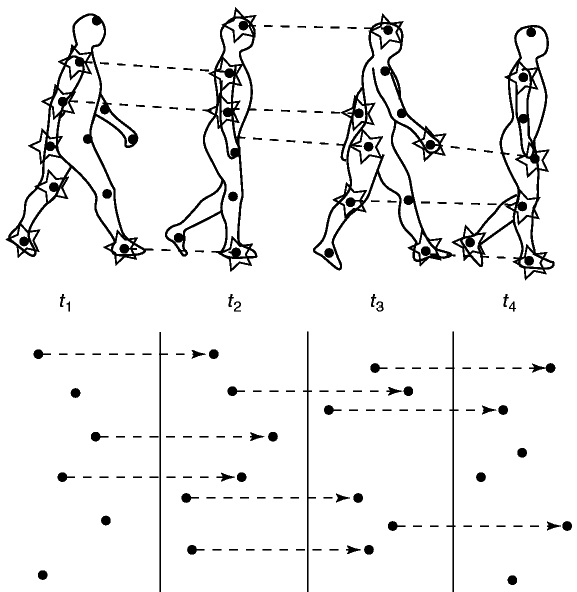
\includegraphics[width=\linewidth]{tseries.jpg}
  \caption{Time series of human motion}
  \label{fig:marginfig}
\end{marginfigure}

\marginnote[300pt]{
In Euclidean geometry, a translation is a function that moves every point a constant distance in a specified direction.  A translation can be described as a rigid motion: other rigid motions include rotations and reflections. A translation can also be interpreted as the addition of a constant vector to every point, or as shifting the origin of the coordinate system.}




\vspace{1cm}


\section{Translational Motion in Space and Time}
Translation is the movement associated with a point particle.  An extended body can have rotational motion and deformations.  When a particle moves through space we describe its motion by collecting ordered pairs of position vectors and times.  This is known as a time series.  Algebraically this corresponds to and x,y,z and t value.  Geometrically this is equivalent to a point in space and a point in time.  These pairs can be considered part of a continuos function.



$$\{\overrightarrow{\scriptr},t\}\ni\overrightarrow{\scriptr}(t)$$

\begin{figure}%

\tdplotsetmaincoords{60}{110}
$$\begin{tikzpicture}[scale=1,tdplot_main_coords]
\coordinate (O) at (0,0,0);
\coordinate (P) at (1,2,3);

\draw[thick,->] (0,0,0) -- (4,0,0) node[anchor=north east]{$x$};
\draw[thick,->] (0,0,0) -- (0,4,0) node[anchor=north west]{$y$};
\draw[thick,->] (0,0,0) -- (0,0,4) node[anchor=south]{$z$};

%draw a vector from origin to point (P) 
\draw[-stealth,very thick,color=red] (O) -- (P) node[anchor=south,color=black]{$\overrightarrow{\scriptr}(t)$};


%draw projection on xy plane, and a connecting line
%syntax: \tdplotdrawarc[coordinate frame, draw options]{center point}{r}{angle}{label options}{label}
%\tdplotdrawarc{(O)}{0.2}{0}{\phivec}{anchor=north}{$\phi$}


%set the rotated coordinate system so the x'-y' plane lies within the
%"theta plane" of the main coordinate system
%syntax: \tdplotsetthetaplanecoords{\phi}
%\tdplotsetthetaplanecoords{\phivec}

%draw theta arc and label, using rotated coordinate system
%\tdplotdrawarc[tdplot_rotated_coords]{(0,0,0)}{0.5}{0}{\thetavec}{anchor=south west}{$\theta$}

\end{tikzpicture}
\hspace{1cm}
\begin{tikzpicture}[scale=1.2]
\draw[thick,->,white] (0,0) -- (4,0) node[anchor=north]{$t$};
\draw[thick,-latex] (0,2) -- (4,2) node[anchor=north]{$t$};
\fill[black] (0.25,2) circle (0.5mm) node [anchor=south ,scale=1] {$0$};
    \fill[black] (2.25,2) circle (0.5mm) node [anchor=south ,scale=1] {$t$};
\end{tikzpicture}$$


  \caption{Geometric position and time}
  \label{fig:marginfig}
\end{figure}


\subsection{Displacement and Time Lapse}
Applying the delta operator $\Delta$ to spatial vector and time series yields the displacement vector and elapsed time.  The vector difference between points in space is known as displacement.  In the temporal dimension the difference between points represents time elapsed.
\begin{marginfigure}[0pt]%
  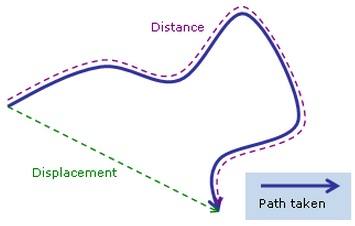
\includegraphics[width=\linewidth]{disp.jpg}
  \caption{Displacement, path and distance traveled}
  \label{fig:marginfig}
\end{marginfigure}
$$\Delta \overrightarrow{\scriptr}=\overrightarrow{\scriptr}_b-\overrightarrow{\scriptr}_a$$
$$\Delta t = t_b-t_a$$
A displacement is the shortest distance from the initial to the final position of a point.  Thus, it is the length of an imaginary straight path, typically distinct from the path actually travelled. A displacement vector represents the length and direction of this imaginary straight path.  A displacement may be also described as a 'relative position': the final position of a point relative to its initial position, and a displacement vector can be mathematically defined as the difference between the final and initial position vectors.




\begin{figure}
\tdplotsetmaincoords{60}{110}
$$\begin{tikzpicture}[scale=1,tdplot_main_coords]
\coordinate (O) at (0,0,0);
\coordinate (P) at (1,2,3);
\coordinate (T) at (1,3,2);

\draw[thick,->] (0,0,0) -- (4,0,0) node[anchor=north east]{$x$};
\draw[thick,->] (0,0,0) -- (0,4,0) node[anchor=north west]{$y$};
\draw[thick,->] (0,0,0) -- (0,0,4) node[anchor=south]{$z$};

%draw a vector from origin to point (P) 
\draw[-stealth,very thick,color=red] (P) -- (T) node[midway,anchor=south west,color=black]{\footnotesize$\Delta\overrightarrow{\scriptr}$};
\draw[-stealth,thick,color=red] (O) -- (T) node[anchor=north,color=black]{\footnotesize$\overrightarrow{\scriptr}_b$};
\draw[-stealth,thick,color=red] (O) -- (P) node[anchor=south east,color=black]{\footnotesize$\overrightarrow{\scriptr}_a$};


%draw projection on xy plane, and a connecting line
%syntax: \tdplotdrawarc[coordinate frame, draw options]{center point}{r}{angle}{label options}{label}
%\tdplotdrawarc{(O)}{0.2}{0}{\phivec}{anchor=north}{$\phi$}


%set the rotated coordinate system so the x'-y' plane lies within the
%"theta plane" of the main coordinate system
%syntax: \tdplotsetthetaplanecoords{\phi}
%\tdplotsetthetaplanecoords{\phivec}

%draw theta arc and label, using rotated coordinate system
%\tdplotdrawarc[tdplot_rotated_coords]{(0,0,0)}{0.5}{0}{\thetavec}{anchor=south west}{$\theta$}

\end{tikzpicture}
\hspace{1cm}
\begin{tikzpicture}[scale=1.2]
\draw[thick,->,white] (0,0) -- (4,0) node[anchor=north]{$t$};
\draw[thick,-latex] (0,2) -- (4,2) node[anchor=north]{$t$};
%\fill[black] (0.25,2) circle (0.5mm) node [anchor=north ,scale=1] {$0$};
    \fill[black] (2,2) circle (0.5mm) node [anchor=north ,scale=1] {$t_a$};
      \fill[black] (3,2) circle (0.5mm) node [anchor=north ,scale=1] {$t_b$};
      \draw[thick,->] (2,2.25) -- (3,2.25) node[midway,anchor=south]{\footnotesize$\Delta t$};
\end{tikzpicture}$$
 \caption{Geometric displacement and elapsed time}
  \label{fig:marginfig}
\end{figure}

Algebraically this corresponds to and $(\Delta x,\Delta y,\Delta z)$ and t value.  Geometrically this is equivalent to a vector in space and a elapse of time.
$$\Delta \overrightarrow{\scriptr}=\Delta x \hat{x}+\Delta y\hat{y}+\Delta z\hat{z}=\left(\begin{array}{c} \Delta x \\ \Delta y \\ \Delta z\end{array}\right)$$

\subsection{Average Velocity}
Average velocity is defined as the displacement vector divided by the elapsed time.  It is a time rate vector pointing in the direction of the displacement.
$$\bar{\overrightarrow{v}}=<\overrightarrow{v}>=\frac{\Delta \overrightarrow{\scriptr}}{\Delta t}$$


\begin{figure}
\tdplotsetmaincoords{60}{110}
$$\begin{tikzpicture}[scale=1,tdplot_main_coords]
\coordinate (O) at (0,0,0);
\coordinate (P) at (1,2,3);
\coordinate (T) at (1,2.4,2.6);

\draw[thick,->] (0,0,0) -- (4,0,0) node[anchor=north east]{$x$};
\draw[thick,->] (0,0,0) -- (0,4,0) node[anchor=north west]{$y$};
\draw[thick,->] (0,0,0) -- (0,0,4) node[anchor=south]{$z$};

%draw a vector from origin to point (P) 
\draw[-stealth,very thick,color=blue] (P) -- (T) node[midway,anchor=south west,color=black]{\footnotesize$\Delta\overrightarrow{\scriptr}=\braket{\overrightarrow{v}}(t) \Delta t$};
\draw[-stealth, thick,color=red] (O) -- (T) node[anchor=north west,color=black]{\footnotesize$\overrightarrow{\scriptr}(t+\Delta t)$};
\draw[-stealth, thick,color=red] (O) -- (P) node[anchor=east,color=black]{\footnotesize$\overrightarrow{\scriptr}(t)$};


%draw projection on xy plane, and a connecting line
%syntax: \tdplotdrawarc[coordinate frame, draw options]{center point}{r}{angle}{label options}{label}
%\tdplotdrawarc{(O)}{0.2}{0}{\phivec}{anchor=north}{$\phi$}


%set the rotated coordinate system so the x'-y' plane lies within the
%"theta plane" of the main coordinate system
%syntax: \tdplotsetthetaplanecoords{\phi}
%\tdplotsetthetaplanecoords{\phivec}

%draw theta arc and label, using rotated coordinate system
%\tdplotdrawarc[tdplot_rotated_coords]{(0,0,0)}{0.5}{0}{\thetavec}{anchor=south west}{$\theta$}

\end{tikzpicture}
\hspace{1cm}
\begin{tikzpicture}[scale=1.2]
\draw[thick,->,white] (0,0) -- (4,0) node[anchor=north]{$t$};
\draw[thick,-latex] (0,2) -- (4,2) node[anchor=north]{$t$};
%\fill[black] (0.25,2) circle (0.5mm) node [anchor=north ,scale=1] {\footnotesize$0$};
    \fill[black] (2,2) circle (0.5mm) node [anchor=north ,scale=1] {\footnotesize$t$};
      \fill[black] (2.4,2) circle (0.5mm) node [anchor=north west ,scale=1] {\footnotesize$t+\Delta t$};
      \draw[thick,->] (2,2.25) -- (2.4,2.25) node[midway,anchor=south]{\footnotesize$\Delta t$};
\end{tikzpicture}$$
 \caption{Geometric displacement as average velocity times elapsed time}
  \label{fig:marginfig}
\end{figure}

Position is described by a three dimensional vector space.  Velocity too can be described by a three dimensional vector space.  The dimensions of velocity space are distance over time.  Since they are distant we should not technically draw a velocity vector on a position graph.  

\marginnote[-140pt]{An instant, $\lim \Delta t \rightarrow 0$, is an infinitesimal moment in time, a moment whose passage is instantaneous.  The continuous nature of time and its infinite divisibility was addressed by Aristotle in his Physics, where he wrote on Zeno's paradoxes. Scientists, philosophers and artists still seek to define the exact nature of an instant thousands of years later.\\

In physics, a theoretical lower-bound unit of time called the Planck time has been proposed, that being the time required for light to travel a distance of 1 Planck length. The Planck time is theorized to be the smallest time measurement that will ever be possible, roughly $10^{-43}$ seconds. Within the framework of the laws of physics as they are understood today, for times less than one Planck time apart, we can neither measure nor detect any change. As of May 2010, the smallest time interval that was directly measured was on the order of 12 attoseconds ($12 \times 10^{-18}$ seconds), about 1024 times larger than the Planck time. It is therefore physically impossible, with current technology, to determine if any action exists that causes a reaction in "an instant", rather than a reaction occurring after an interval of time too short to observe or measure.}

\subsection{Instantaneous Velocity}
Instantaneous velocity is defined as the average velocity in the limit as ${\Delta t}$ and $\Delta \overrightarrow{\scriptr}$ go to zero.  This is informally notated as $\Delta \rightarrow 0$.
$$\overrightarrow{v}=\lim_{\Delta \rightarrow 0}\frac{\Delta \overrightarrow{\scriptr}}{\Delta t}$$
The instantaneous velocity vector $\overrightarrow{v}$ has a component in the x, y and z directions.
$$\overrightarrow{v}=v_x\hat{x}+v_y\hat{y}+v_z\hat{z}=\left(\begin{array}{c} v_x \\ v_y \\ v_z\end{array}\right)$$

\newpage


\subsection{Change in Velocity}

Applying the delta operator $\Delta$ to the velocity vector yields a change in velocity vector $\Delta \overrightarrow{v}$.  The vector $\Delta \overrightarrow{v}$ is the difference between final velocity state and initial velocity state.  Algebraically this is the final velocity vector $\overrightarrow{v}_b$ minus the initial velocity vector $\overrightarrow{v}_a$.   
$$\Delta \overrightarrow{v}=\overrightarrow{v}_b-\overrightarrow{v}_a$$
Geometrically the change in velocity vector $\Delta \overrightarrow{v}$ represents the vector beginning at the point represented by $\overrightarrow{v}_a$ and ending at $\overrightarrow{v}_b$.  
\begin{figure}
$$\begin{tikzpicture}[scale=1,tdplot_main_coords]


\coordinate (O) at (0,0,0);
\coordinate (P) at (1,2,-3);
\coordinate (T) at (1,3,-2);

\draw[thick,->] (0,0,0) -- (4,0,0) node[anchor=north east]{$v_x$};
\draw[thick,->] (0,0,0) -- (0,4,0) node[anchor=north west]{$v_y$};
\draw[thick,->] (0,0,0) -- (0,0,4) node[anchor=south]{$v_z$};

%draw a vector from origin to point (P) 
\draw[-stealth,very thick,color=blue] (P) -- (T) node[midway,anchor=north west,color=black]{\footnotesize$\Delta\overrightarrow{v}$};
\draw[-stealth,thick,color=blue] (O) -- (T) node[anchor=west,color=black]{\footnotesize$\overrightarrow{v}_b$};
\draw[-stealth,thick,color=blue] (O) -- (P) node[anchor=east,color=black]{\footnotesize$\overrightarrow{v}_a$};


%draw projection on xy plane, and a connecting line
%syntax: \tdplotdrawarc[coordinate frame, draw options]{center point}{r}{angle}{label options}{label}
%\tdplotdrawarc{(O)}{0.2}{0}{\phivec}{anchor=north}{$\phi$}


%set the rotated coordinate system so the x'-y' plane lies within the
%"theta plane" of the main coordinate system
%syntax: \tdplotsetthetaplanecoords{\phi}
%\tdplotsetthetaplanecoords{\phivec}

%draw theta arc and label, using rotated coordinate system
%\tdplotdrawarc[tdplot_rotated_coords]{(0,0,0)}{0.5}{0}{\thetavec}{anchor=south west}{$\theta$}

\end{tikzpicture}
\hspace{1cm}
\begin{tikzpicture}[scale=1.2]
\draw[thick,->,white] (0,0) -- (4,0) node[anchor=north]{$t$};
\draw[thick,-latex] (0,2) -- (4,2) node[anchor=north]{$t$};
%\fill[black] (0.25,2) circle (0.5mm) node [anchor=north ,scale=1] {$0$};
    \fill[black] (2,2) circle (0.5mm) node [anchor=north ,scale=1] {$t_a$};
      \fill[black] (3,2) circle (0.5mm) node [anchor=north ,scale=1] {$t_b$};
      \draw[thick,->] (2,2.25) -- (3,2.25) node[midway,anchor=south]{\footnotesize$\Delta t$};
\end{tikzpicture}$$
 \caption{Geometric velocity and elapsed time}
  \label{fig:marginfig}
\end{figure}



\subsection{Average Acceleration}
Average acceleration is defined as the change in velocity vector divided by the elapsed time.  It is a time rate vector pointing in the direction of changing velocity.
$$\bar{\overrightarrow{a}}=<\overrightarrow{a}>=\frac{\Delta \overrightarrow{v}}{\Delta t}$$

\subsection{Instantaneous Acceleration}
Instantaneous acceleration is defined as the average acceleration in the limit as ${\Delta t}$ and $\Delta \overrightarrow{v}$ go to zero. 
$$\overrightarrow{a}=\lim_{\Delta \rightarrow 0}\frac{\Delta \overrightarrow{v}}{\Delta t}$$
The instantaneous acceleration is a vector with an x, y, and z component.
$$\overrightarrow{a}=a_x\hat{x}+a_y\hat{y}+a_z\hat{z}=\left(\begin{array}{c} a_x \\ a_y \\ a_z\end{array}\right)$$

\begin{figure}
\tdplotsetmaincoords{60}{110}
$$\begin{tikzpicture}[scale=1,tdplot_main_coords]
\coordinate (O) at (0,0,0);
\coordinate (P) at (1,2,-2);
\coordinate (T) at (1,2.4,-1.6);

\draw[thick,->] (0,0,0) -- (4,0,0) node[anchor=north east]{$v_x$};
\draw[thick,->] (0,0,0) -- (0,4,0) node[anchor=north west]{$v_y$};
\draw[thick,->] (0,0,0) -- (0,0,4) node[anchor=south]{$v_z$};

%draw a vector from origin to point (P) 
\draw[-stealth,very thick,color=green] (P) -- (T) node[midway,anchor=north west,color=black]{\footnotesize$\Delta \overrightarrow{v}=\braket{\overrightarrow{a}(t)} \Delta t$};
\draw[-stealth, thick,color=blue] (O) -- (T) node[anchor=south west,color=black]{\footnotesize$\overrightarrow{v}(t+\Delta t)$};
\draw[-stealth, thick,color=blue] (O) -- (P) node[anchor=east,color=black]{\footnotesize$\overrightarrow{v}(t)$};


%draw projection on xy plane, and a connecting line
%syntax: \tdplotdrawarc[coordinate frame, draw options]{center point}{r}{angle}{label options}{label}
%\tdplotdrawarc{(O)}{0.2}{0}{\phivec}{anchor=north}{$\phi$}


%set the rotated coordinate system so the x'-y' plane lies within the
%"theta plane" of the main coordinate system
%syntax: \tdplotsetthetaplanecoords{\phi}
%\tdplotsetthetaplanecoords{\phivec}

%draw theta arc and label, using rotated coordinate system
%\tdplotdrawarc[tdplot_rotated_coords]{(0,0,0)}{0.5}{0}{\thetavec}{anchor=south west}{$\theta$}

\end{tikzpicture}
\hspace{1cm}
\begin{tikzpicture}[scale=1.2]
\draw[thick,->,white] (0,0) -- (4,0) node[anchor=north]{$t$};
\draw[thick,-latex] (0,2) -- (4,2) node[anchor=north]{$t$};
\fill[black] (0.25,2) circle (0.5mm) node [anchor=north ,scale=1] {\footnotesize$0$};
    \fill[black] (2,2) circle (0.5mm) node [anchor=north ,scale=1] {\footnotesize$t$};
      \fill[black] (2.4,2) circle (0.5mm) node [anchor=north west ,scale=1] {\footnotesize$t+\Delta t$};
      \draw[thick,->] (2,2.25) -- (2.4,2.25) node[midway,anchor=south]{\footnotesize$\Delta t$};
\end{tikzpicture}$$
 \caption{Geometric position and time}
  \label{fig:marginfig}
\end{figure}

\begin{fullwidth}
In mathematics, infinitesimals are things so small that there is no way to measure them. The insight with exploiting infinitesimals was that entities could still retain certain specific properties, such as angle or slope, even though these entities were quantitatively small.  The word infinitesimal comes from a 17th-century Modern Latin coinage infinitesimus, which originally referred to the "infinite-th" item in a sequence. It was originally introduced around 1670 by either Nicolaus Mercator or Gottfried Wilhelm Leibniz.  Infinitesimals are a basic ingredient in the procedures of infinitesimal calculus as developed by Leibniz, including the law of continuity and the transcendental law of homogeneity. In common speech, an infinitesimal object is an object which is smaller than any feasible measurement, but not zero in size; or, so small that it cannot be distinguished from zero by any available means. Hence, when used as an adjective, "infinitesimal" means "extremely small". In order to give it a meaning it usually has to be compared to another infinitesimal object in the same context (as in a derivative). Infinitely many infinitesimals are summed to produce an integral.
\end{fullwidth}

\newpage
\section{Kinematic Difference: Slope and Curvature}
\begin{marginfigure}[20pt]%
  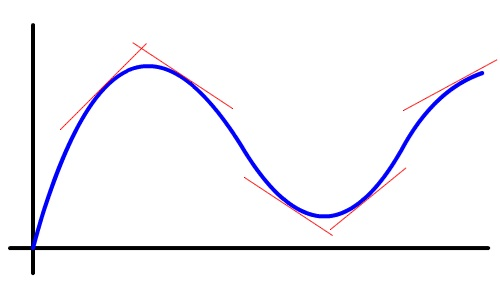
\includegraphics[width=\linewidth]{tangent.jpg}
  \caption{Tangent lines of a function}
  \label{fig:marginfig}
\end{marginfigure}
\subsubsection{Velocity}
In one dimensional motion there is only one degree of freedom, represented by the variable $x$.  When $x$ is graphed against $t$ in a position vs time graph the velocity is represented by the slope of the tangent line of $x(t)$.
$$v=\text{Slope of tangent line on position vs time graph}$$
$$v=\lim_{\Delta \rightarrow 0}\frac{\Delta x}{ \Delta t}$$
\begin{marginfigure}[40pt]%
  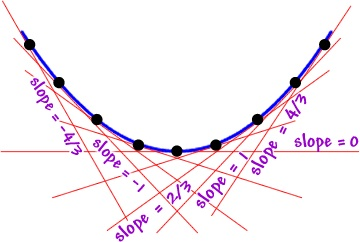
\includegraphics[width=\linewidth]{curve.jpg}
  \caption{Curvature of a function}
  \label{fig:marginfig}
\end{marginfigure}
\subsubsection{Acceleration}

When $v$ is graphed against $t$ in a velocity vs time graph the acceleration is represented by the slope of the tangent line of $v(t)$.  Acceleration is the time rate of change of the velocity.
$$a=\text{Slope of the tangent line on the velocity vs time graph}$$
$$a=\lim_{\Delta \rightarrow 0}\frac{\Delta v}{ \Delta t}$$
\begin{marginfigure}[60pt]%
  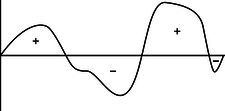
\includegraphics[width=\linewidth]{area.jpg}
  \caption{Area under a function}
  \label{fig:marginfig}
\end{marginfigure}
The acceleration is the rate of change of the velocity and the velocity is the slope of $x(t)$.  Therefore the acceleration is the rate of change of the slope, namely it is the curvature.
$$a=\text{Curvature on the position vs time graph}$$
$$a=\lim_{\Delta \rightarrow 0}\frac{\Delta \left( \nicefrac{\Delta x}{\Delta t}\right)}{ \Delta t}$$

\section{Kinematic Accumulation: Area Under Curve}
\subsubsection{Position}
\marginnote[30pt]{When $v$ is graphed against $t$ in a velocity vs time graph the displacement $\Delta x$ is the area under the graph of $v(t)$.  The displacement from the initial position $x(0)$ gives position as a function of time $x(t)$.}
$$\Delta x=\text{Area under velocity vs time graph}$$
$$\Delta x=\braket{v} \Delta t$$
$$x(t)=x(0)+\Delta x$$

\subsubsection{Velocity}
\marginnote[20pt]{When $a$ is graphed against $t$ in an acceleration vs time graph the change in velocity $\Delta v$ is the area under the graph of $a(t)$.  The change from the initial velocity $v(0)$ gives velocity as a function of time $v(t)$.}
$$\Delta v=\text{Area under acceleration vs time graph}$$
$$\Delta v=\braket{a} \Delta t$$
$$v(t)=v(0)+\Delta v$$



\newpage
\subsubsection{Graphical Representation}

\vspace{1cm}
\marginnote[50pt]{The slope of the tangent lines of the acceleration function is known as the jerk.  The area under the acceleration function is the change in velocity.  The change may be computed from the t=0 or an arbitrary time. }
\marginnote[125pt]{The slope of the tangent lines of the velocity function is the acceleration.  The area under the velocity function is the change in position, or displacement.  The change may be computed from the t=0 or an arbitrary time. }
\marginnote[125pt]{The slope of the tangent lines of the position function is the velocity.  The area under the position function is not physically meaningful. }
$$
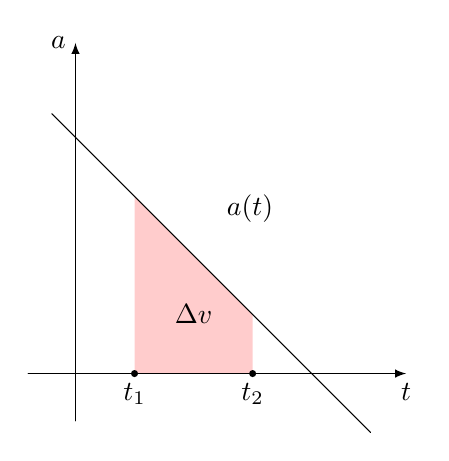
\begin{tikzpicture}
    [line cap=round,line join=round,x=2cm,y=2cm, scale=1.5, decoration={brace,amplitude=2pt}]
%main layer
%creating the ticks and xy-axis nodes
%some function
\fill[fill=red!20] (0.25,0) -- plot [domain=0.25:.75] (\x,{1-\x}) -- plot [domain=0.75: 0.25] (\x,0) -- cycle;

 \draw[smooth,samples=100,domain=-0.1:1.25]
                                 plot(\x,{1-\x});
 
  %\draw [darkgray,ultra thin] (0,0.479)-- (0.25,0.479);
  %\draw [darkgray,ultra thin] (0,0.938)-- (0.75,0.938);
 % \draw [darkgray,ultra thin] (0.25,0.479)-- (0.25,0.0);
  %\draw [darkgray,ultra thin] (0.75,0.938)-- (0.75,0);
%creating the curly braces with decorate
 
%  \draw [decorate,color=black!80!black] (0.25,0.0)--(0.75,0.0)
   %node [midway,anchor=north,inner sep=1pt, outer sep=1pt]{\small$\Delta x$};
    \fill[black] (0.25,0) circle (0.3mm) node [anchor=north ,scale=1] {$ t_1$};
     \fill[black] (0.75,0) circle (0.3mm) node [anchor=north ,scale=1] {$t_2$};

  \draw[-latex,color=black,thin] (-0.2,0) -- (1.4,0) node [anchor=north ,scale=1] {$t$};
   \draw[-latex,color=black,thin] (0,-0.2) -- (0,1.4)node [anchor=east ,scale=1] {$a$};
    \draw (0.6,0.6) node [anchor=south west ,scale=1] {$a(t)$};
        \draw (0.5,0.25) node [anchor=center ,scale=1] {$\Delta v$};
        
 \end{tikzpicture}
 \hspace{1cm}
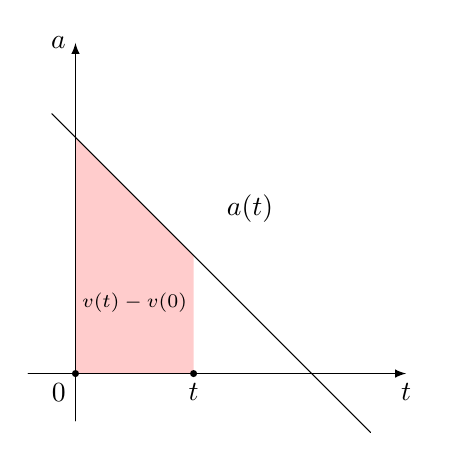
\begin{tikzpicture}
    [line cap=round,line join=round,x=2cm,y=2cm, scale=1.5, decoration={brace,amplitude=2pt}]
%main layer
%creating the ticks and xy-axis nodes
%some function
\fill[fill=red!20] (0,0) -- plot [domain=0:.5] (\x,{1-\x}) -- plot [domain=0.5: 0.0] (\x,0) -- cycle;

 \draw[smooth,samples=100,domain=-0.1:1.25]
                                 plot(\x,{1-\x});
 
  %\draw [darkgray,ultra thin] (0,0.479)-- (0.25,0.479);
  %\draw [darkgray,ultra thin] (0,0.938)-- (0.75,0.938);
 % \draw [darkgray,ultra thin] (0.25,0.479)-- (0.25,0.0);
  %\draw [darkgray,ultra thin] (0.75,0.938)-- (0.75,0);
%creating the curly braces with decorate
 
%  \draw [decorate,color=black!80!black] (0.25,0.0)--(0.75,0.0)
   %node [midway,anchor=north,inner sep=1pt, outer sep=1pt]{\small$\Delta x$};
    \fill[black] (0,0) circle (0.3mm) node [anchor=north east,scale=1] {$ 0$};
     \fill[black] (0.5,0) circle (0.3mm) node [anchor=north ,scale=1] {$t$};

  \draw[-latex,color=black,thin] (-0.2,0) -- (1.4,0) node [anchor=north ,scale=1] {$t$};
   \draw[-latex,color=black,thin] (0,-0.2) -- (0,1.4)node [anchor=east ,scale=1] {$a$};
    \draw (0.6,0.6) node [anchor=south west ,scale=1] {$a(t)$};
        \draw (0.25,0.3) node [anchor=center ,scale=1] {\scriptsize$v(t)-v(0)$};
        
 \end{tikzpicture}
$$
\vspace{1cm}
$$
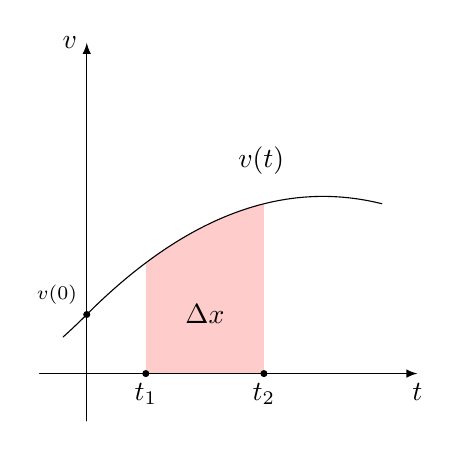
\begin{tikzpicture}
    [line cap=round,line join=round,x=2cm,y=2cm, scale=1.5, decoration={brace,amplitude=2pt}]
%main layer
%creating the ticks and xy-axis nodes
%some function
\fill[fill=red!20] (0.25,0) -- plot [domain=0.25:.75] (\x,{-\x^2/2+\x+0.25}) -- plot [domain=0.75: 0.25] (\x,0) -- cycle;

 \draw[smooth,samples=100,domain=-0.1:1.25]
                                 plot(\x,{-\x^2/2+\x+0.25});
 
  %\draw [darkgray,ultra thin] (0,0.479)-- (0.25,0.479);
  %\draw [darkgray,ultra thin] (0,0.938)-- (0.75,0.938);
 % \draw [darkgray,ultra thin] (0.25,0.479)-- (0.25,0.0);
  %\draw [darkgray,ultra thin] (0.75,0.938)-- (0.75,0);
%creating the curly braces with decorate
 
%  \draw [decorate,color=black!80!black] (0.25,0.0)--(0.75,0.0)
   %node [midway,anchor=north,inner sep=1pt, outer sep=1pt]{\small$\Delta x$};
    \fill[black] (0.25,0) circle (0.3mm) node [anchor=north ,scale=1] {$ t_1$};
     \fill[black] (0.75,0) circle (0.3mm) node [anchor=north ,scale=1] {$t_2$};
        \fill[black] (0,0.25) circle (0.3mm) node [anchor=south east,scale=1] {\scriptsize$ v(0)$};

  \draw[-latex,color=black,thin] (-0.2,0) -- (1.4,0) node [anchor=north ,scale=1] {$t$};
   \draw[-latex,color=black,thin] (0,-0.2) -- (0,1.4)node [anchor=east ,scale=1] {$v$};
    \draw (0.6,0.8) node [anchor=south west ,scale=1] {$v(t)$};
        \draw (0.5,0.25) node [anchor=center ,scale=1] {$\Delta x$};
        
 \end{tikzpicture}
 \hspace{1cm}
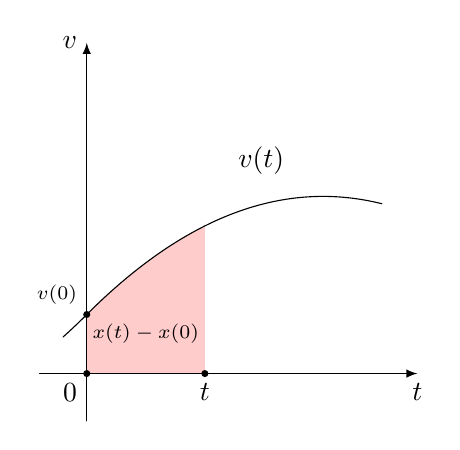
\begin{tikzpicture}
    [line cap=round,line join=round,x=2cm,y=2cm, scale=1.5, decoration={brace,amplitude=2pt}]
%main layer
%creating the ticks and xy-axis nodes
%some function
\fill[fill=red!20] (0,0) -- plot [domain=0:.5] (\x,{-\x^2/2+\x+0.25}) -- plot [domain=0.5: 0.0] (\x,0) -- cycle;

 \draw[smooth,samples=100,domain=-0.1:1.25]
                                 plot(\x,{-\x^2/2+\x+0.25});
 
  %\draw [darkgray,ultra thin] (0,0.479)-- (0.25,0.479);
  %\draw [darkgray,ultra thin] (0,0.938)-- (0.75,0.938);
 % \draw [darkgray,ultra thin] (0.25,0.479)-- (0.25,0.0);
  %\draw [darkgray,ultra thin] (0.75,0.938)-- (0.75,0);
%creating the curly braces with decorate
 
%  \draw [decorate,color=black!80!black] (0.25,0.0)--(0.75,0.0)
   %node [midway,anchor=north,inner sep=1pt, outer sep=1pt]{\small$\Delta x$};
    \fill[black] (0,0) circle (0.3mm) node [anchor=north east,scale=1] {$ 0$};
     \fill[black] (0.5,0) circle (0.3mm) node [anchor=north ,scale=1] {$t$};
      \fill[black] (0,0.25) circle (0.3mm) node [anchor=south east,scale=1] {\scriptsize$ v(0)$};

  \draw[-latex,color=black,thin] (-0.2,0) -- (1.4,0) node [anchor=north ,scale=1] {$t$};
   \draw[-latex,color=black,thin] (0,-0.2) -- (0,1.4)node [anchor=east ,scale=1] {$v$};
     \draw (0.6,0.8) node [anchor=south west ,scale=1] {$v(t)$};
        \draw (0.25,0.25) node [anchor=north ,scale=1] {\scriptsize$x(t)-x(0)$};
        
 \end{tikzpicture}
$$
\vspace{1cm}
$$
\begin{tikzpicture}
    [line cap=round,line join=round,x=2cm,y=2cm, scale=1.5, decoration={brace,amplitude=2pt}]
%main layer
%creating the ticks and xy-axis nodes
%some function
%\fill[fill=red!20] (0.25,0) -- plot [domain=0.25:.75] (\x,{-\x^3/6+\x^2/2+0.25\x+0.1}) -- plot [domain=0.75: 0.25] (\x,0) -- cycle;

 \draw[smooth,samples=100,domain=-0.1:1.25]
                                 plot(\x,{-\x^3/6+\x^2/2+\x/4+0.1});
 
  %\draw [darkgray,ultra thin] (0,0.479)-- (0.25,0.479);
  %\draw [darkgray,ultra thin] (0,0.938)-- (0.75,0.938);
 % \draw [darkgray,ultra thin] (0.25,0.479)-- (0.25,0.0);
  %\draw [darkgray,ultra thin] (0.75,0.938)-- (0.75,0);
%creating the curly braces with decorate
 
%  \draw [decorate,color=black!80!black] (0.25,0.0)--(0.75,0.0)
   %node [midway,anchor=north,inner sep=1pt, outer sep=1pt]{\small$\Delta x$};
           \fill[black] (0,0.1) circle (0.3mm) node [anchor=south east,scale=1] {\scriptsize$ x(0)$};

  \draw[-latex,color=black,thin] (-0.2,0) -- (1.4,0) node [anchor=north ,scale=1] {$t$};
   \draw[-latex,color=black,thin] (0,-0.2) -- (0,1.4)node [anchor=east ,scale=1] {$x$};
    \draw (0.6,0.8) node [anchor=south west ,scale=1] {$x(t)$};
              
 \end{tikzpicture}
 \hspace{1cm}
\begin{tikzpicture}
    [line cap=round,line join=round,x=2cm,y=2cm, scale=1.5, decoration={brace,amplitude=2pt}]
%main layer
%creating the ticks and xy-axis nodes
%some function
%\fill[fill=red!20] (0,0) -- plot [domain=0:.5] (\x,{-\x^2/2+\x+0.25}) -- plot [domain=0.5: 0.0] (\x,0) -- cycle;

 \draw[smooth,samples=100,domain=-0.1:1.25]
                                 plot(\x,{-\x^3/6+\x^2/2+\x/4+0.1});

 
  %\draw [darkgray,ultra thin] (0,0.479)-- (0.25,0.479);
  %\draw [darkgray,ultra thin] (0,0.938)-- (0.75,0.938);
 % \draw [darkgray,ultra thin] (0.25,0.479)-- (0.25,0.0);
  %\draw [darkgray,ultra thin] (0.75,0.938)-- (0.75,0);
%creating the curly braces with decorate
 
%  \draw [decorate,color=black!80!black] (0.25,0.0)--(0.75,0.0)
   %node [midway,anchor=north,inner sep=1pt, outer sep=1pt]{\small$\Delta x$};
  
      \fill[black] (0,0.1) circle (0.3mm) node [anchor=south east,scale=1] {\scriptsize$ x(0)$};

  \draw[-latex,color=black,thin] (-0.2,0) -- (1.4,0) node [anchor=north ,scale=1] {$t$};
   \draw[-latex,color=black,thin] (0,-0.2) -- (0,1.4)node [anchor=east ,scale=1] {$x$};
     \draw (0.6,0.8) node [anchor=south west ,scale=1] {$x(t)$};
       % \draw (0.25,0.25) node [anchor=center ,scale=1] {\scriptsize$x(t)-x(0)$};
        
 \end{tikzpicture}
$$
\newpage

\section{Simple 1-D Motion}
\subsection{Constant Velocity}
\marginnote[50pt]{The situation of constant velocity means it is not changing or its rate of change is zero.  Constant velocity is zero acceleration.  Zero acceleration yields no area under the curve.  $\Delta v=0$ }
\marginnote[190pt]{Since the velocity doesn't change $\Delta v=0$ and the velocity stays as $v_0$, all day everyday. }
\marginnote[160pt]{If the velocity is constant the slope of $x(t)$ is constant.   It is a straight line with a slope $v_0$ and vertical intercept of $x_0$ . The curvature is zero. }
\begin{center}
\begin{tabular}{cc}
\begin{minipage}{5cm}
$$a(t)=\text{Slope}(v(t))=0$$
%$$\bar{a}=0$$
$$\Delta v=\text{Area under }a(t)=0$$
%$$\Delta v=\bar{a}\Delta t=0$$
$$v(t)=v(0)+\Delta v$$
$$v(t)=v(0)$$
\end{minipage}
&
\begin{minipage}{5cm}
$$\begin{tikzpicture}
    [line cap=round,line join=round,x=2cm,y=2cm, scale=1.5, decoration={brace,amplitude=2pt}]
%main layer
%creating the ticks and xy-axis nodes
%some function

 
  %\draw [darkgray,ultra thin] (0,0.479)-- (0.25,0.479);
  %\draw [darkgray,ultra thin] (0,0.938)-- (0.75,0.938);
 % \draw [darkgray,ultra thin] (0.25,0.479)-- (0.25,0.0);
  %\draw [darkgray,ultra thin] (0.75,0.938)-- (0.75,0);
%creating the curly braces with decorate
 
%  \draw [decorate,color=black!80!black] (0.25,0.0)--(0.75,0.0)
   %node [midway,anchor=north,inner sep=1pt, outer sep=1pt]{\small$\Delta x$};
   

  \draw[-latex,color=black,thin] (-0.2,0) -- (1.4,0) node [anchor=north ,scale=1] {$t$};
   \draw[-latex,color=black,thin] (0,-0.2) -- (0,1.4)node [anchor=east ,scale=1] {$a$};
    \draw (0.6,0.6) node [anchor=south west ,scale=1] {\scriptsize$a(t)=0$};
      %  \draw (0.25,0.3) node [anchor=west ,scale=1] {\scriptsize$v(t)-v(0)=\int a(t)dt=0$};
        
 \end{tikzpicture}$$
 \end{minipage}
 \end{tabular}
 \end{center}
 
 \vspace{1cm}
 \begin{center}
\begin{tabular}{cc}
\begin{minipage}{5cm}
$$v(t)=v(0)=v_0=\text{constant}$$
$$v(t)=\text{Slope}(x(t))$$
$$\Delta x=\text{Area under }v(t)$$
$$\Delta x=v_0 \Delta t$$
$$x(t)=x(0)+v_0 t$$

\end{minipage}
&
\begin{minipage}{5cm}
$$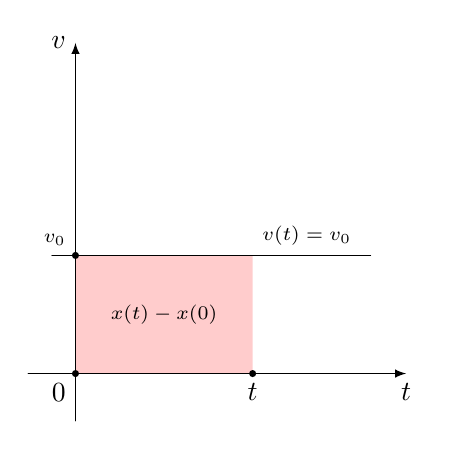
\begin{tikzpicture}
    [line cap=round,line join=round,x=2cm,y=2cm, scale=1.5, decoration={brace,amplitude=2pt}]
%main layer
%creating the ticks and xy-axis nodes
%some function
\fill[fill=red!20] (0,0) -- plot [domain=0:.75] (\x,0.5) -- plot [domain=0.75: 0.0] (\x,0) -- cycle;

 \draw[smooth,samples=100,domain=-0.1:1.25]
                                 plot(\x,0.5);
 
  %\draw [darkgray,ultra thin] (0,0.479)-- (0.25,0.479);
  %\draw [darkgray,ultra thin] (0,0.938)-- (0.75,0.938);
 % \draw [darkgray,ultra thin] (0.25,0.479)-- (0.25,0.0);
  %\draw [darkgray,ultra thin] (0.75,0.938)-- (0.75,0);
%creating the curly braces with decorate
 
%  \draw [decorate,color=black!80!black] (0.25,0.0)--(0.75,0.0)
   %node [midway,anchor=north,inner sep=1pt, outer sep=1pt]{\small$\Delta x$};
    \fill[black] (0,0) circle (0.3mm) node [anchor=north east,scale=1] {$ 0$};
     \fill[black] (0.75,0) circle (0.3mm) node [anchor=north ,scale=1] {$t$};
      \fill[black] (0,0.5) circle (0.3mm) node [anchor=south east,scale=1] {\scriptsize$ v_0$};

  \draw[-latex,color=black,thin] (-0.2,0) -- (1.4,0) node [anchor=north ,scale=1] {$t$};
   \draw[-latex,color=black,thin] (0,-0.2) -- (0,1.4)node [anchor=east ,scale=1] {$v$};
     \draw (0.75,0.5) node [anchor=south west ,scale=1] {\scriptsize$v(t)=v_0$};
        \draw (0.375,0.25) node [anchor=center ,scale=1] {\scriptsize$x(t)-x(0)$};
        
 \end{tikzpicture}
$$

  \end{minipage}
 \end{tabular}
 \end{center}
 

 \vspace{1cm}
 \begin{center}
\begin{tabular}{cc}
\begin{minipage}{5cm}
 

$$x(t)=x_0+v_0t$$

\end{minipage}
&
\begin{minipage}{5cm}

$$\begin{tikzpicture}
    [line cap=round,line join=round,x=2cm,y=2cm, scale=1.5, decoration={brace,amplitude=2pt}]
%main layer
%creating the ticks and xy-axis nodes
%some function
%\fill[fill=red!20] (0,0) -- plot [domain=0:.5] (\x,{-\x^2/2+\x+0.25}) -- plot [domain=0.5: 0.0] (\x,0) -- cycle;

 \draw[smooth,samples=100,domain=-0.1:1.25]
                                 plot(\x,{0.25+\x/2});

 
  %\draw [darkgray,ultra thin] (0,0.479)-- (0.25,0.479);
  %\draw [darkgray,ultra thin] (0,0.938)-- (0.75,0.938);
 % \draw [darkgray,ultra thin] (0.25,0.479)-- (0.25,0.0);
  %\draw [darkgray,ultra thin] (0.75,0.938)-- (0.75,0);
%creating the curly braces with decorate
 
%  \draw [decorate,color=black!80!black] (0.25,0.0)--(0.75,0.0)
   %node [midway,anchor=north,inner sep=1pt, outer sep=1pt]{\small$\Delta x$};
  
      \fill[black] (0,0.25) circle (0.3mm) node [anchor=south east,scale=1] {\scriptsize$ x_0$};

  \draw[-latex,color=black,thin] (-0.2,0) -- (1.4,0) node [anchor=north ,scale=1] {$t$};
   \draw[-latex,color=black,thin] (0,-0.2) -- (0,1.4)node [anchor=east ,scale=1] {$x$};
     \draw (0.75,0.9) node [anchor=center ,scale=1] {\scriptsize$x(t)=x_0+v_0t$};
       % \draw (0.25,0.25) node [anchor=center ,scale=1] {\scriptsize$x(t)-x(0)$};
        
 \end{tikzpicture}
$$
 \end{minipage}
 \end{tabular}
 \end{center}
\newpage
\subsection{Constant Acceleration}
\marginnote[50pt]{Constant acceleration is smooth, zero jerk.  It generates a rectangular area beneath it representing the change in velocity.  $\text{Area}=\text{height}\times\text{base}$ so $\Delta v= a t$.  The acceleration is the average acceleration because it dent change.  It stays constant $a$ all day everyday. }
\marginnote[150pt]{Since the acceleration is constant the slope of the velocity versus time graph is constant.  $v(t)$ is a straight line with slope a. The vertical intercept is $v_0$.  The area underneath the function is the displacement.  It may be computed using the triangular portion $\nicefrac{at^2}{2}$ and rectangular portion $v_0t$. }
\marginnote[160pt]{The slope of $x(t)$ is changing linearly so $x(t)$ is parabolic.   It is a quadratic function with vertical intercept of $x_0$. }
\begin{center}
\begin{tabular}{cc}
\begin{minipage}{5cm}
$$\text{Slope}(a(t))=0$$
$$a(t)=a=\text{constant}$$
$$\Delta v=\text{Area under }a(t)$$
$$\Delta v=at$$
$$v(t)=v(0)+\Delta v$$
$$v(t)=v(0)+at$$

\end{minipage}
&
\begin{minipage}{5cm}
$$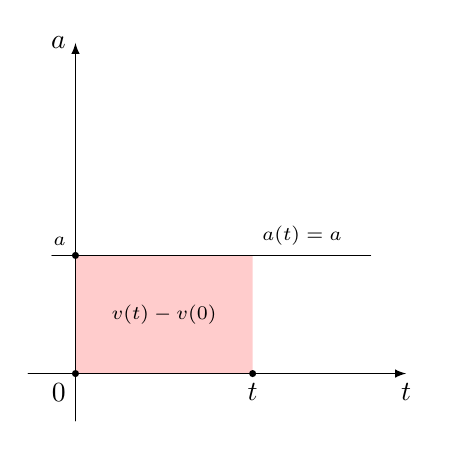
\begin{tikzpicture}
    [line cap=round,line join=round,x=2cm,y=2cm, scale=1.5, decoration={brace,amplitude=2pt}]
%main layer
%creating the ticks and xy-axis nodes
%some function
\fill[fill=red!20] (0,0) -- plot [domain=0:.75] (\x,0.5) -- plot [domain=0.75: 0.0] (\x,0) -- cycle;

 \draw[smooth,samples=100,domain=-0.1:1.25]
                                 plot(\x,0.5);
 
  %\draw [darkgray,ultra thin] (0,0.479)-- (0.25,0.479);
  %\draw [darkgray,ultra thin] (0,0.938)-- (0.75,0.938);
 % \draw [darkgray,ultra thin] (0.25,0.479)-- (0.25,0.0);
  %\draw [darkgray,ultra thin] (0.75,0.938)-- (0.75,0);
%creating the curly braces with decorate
 
%  \draw [decorate,color=black!80!black] (0.25,0.0)--(0.75,0.0)
   %node [midway,anchor=north,inner sep=1pt, outer sep=1pt]{\small$\Delta x$};
    \fill[black] (0,0) circle (0.3mm) node [anchor=north east,scale=1] {$ 0$};
     \fill[black] (0.75,0) circle (0.3mm) node [anchor=north ,scale=1] {$t$};
      \fill[black] (0,0.5) circle (0.3mm) node [anchor=south east,scale=1] {\scriptsize$ a$};

  \draw[-latex,color=black,thin] (-0.2,0) -- (1.4,0) node [anchor=north ,scale=1] {$t$};
   \draw[-latex,color=black,thin] (0,-0.2) -- (0,1.4)node [anchor=east ,scale=1] {$a$};
     \draw (0.75,0.5) node [anchor=south west ,scale=1] {\scriptsize$a(t)=a$};
        \draw (0.375,0.25) node [anchor=center ,scale=1] {\scriptsize$v(t)-v(0)$};
        
 \end{tikzpicture}
$$

 \end{minipage}
 \end{tabular}
 \end{center}
 
 \vspace{1cm}
 \begin{center}
\begin{tabular}{cc}
\begin{minipage}{5cm}
$$v(t)=v_0+at$$
$$v(t)=\text{Slope}(x(t))$$
$$\Delta x=\text{Area under }v(t)$$
$$\Delta x =v_0t+\frac{1}{2}at^2$$
$$x(t)=x(0)+\Delta x$$
$$x(t)=x(0)+v_0t+\frac{1}{2}at^2$$
\end{minipage}
&
\begin{minipage}{5cm}
$$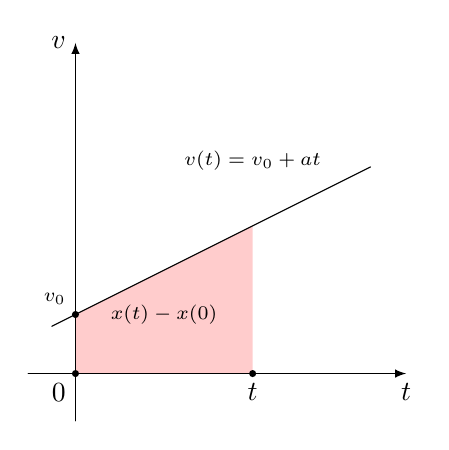
\begin{tikzpicture}
    [line cap=round,line join=round,x=2cm,y=2cm, scale=1.5, decoration={brace,amplitude=2pt}]
%main layer
%creating the ticks and xy-axis nodes
%some function
\fill[fill=red!20] (0,0) -- plot [domain=0:.75] (\x,{\x/2+0.25}) -- plot [domain=0.75: 0.0] (\x,0) -- cycle;

 \draw[smooth,samples=100,domain=-0.1:1.25]
                                 plot(\x,{\x/2+0.25});
 
  %\draw [darkgray,ultra thin] (0,0.479)-- (0.25,0.479);
  %\draw [darkgray,ultra thin] (0,0.938)-- (0.75,0.938);
 % \draw [darkgray,ultra thin] (0.25,0.479)-- (0.25,0.0);
  %\draw [darkgray,ultra thin] (0.75,0.938)-- (0.75,0);
%creating the curly braces with decorate
 
%  \draw [decorate,color=black!80!black] (0.25,0.0)--(0.75,0.0)
   %node [midway,anchor=north,inner sep=1pt, outer sep=1pt]{\small$\Delta x$};
    \fill[black] (0,0) circle (0.3mm) node [anchor=north east,scale=1] {$ 0$};
     \fill[black] (0.75,0) circle (0.3mm) node [anchor=north ,scale=1] {$t$};
      \fill[black] (0,0.25) circle (0.3mm) node [anchor=south east,scale=1] {\scriptsize$ v_0$};

  \draw[-latex,color=black,thin] (-0.2,0) -- (1.4,0) node [anchor=north ,scale=1] {$t$};
   \draw[-latex,color=black,thin] (0,-0.2) -- (0,1.4)node [anchor=east ,scale=1] {$v$};
     \draw (0.75,0.9) node [anchor=center ,scale=1] {\scriptsize$v(t)=v_0+at$};
        \draw (0.375,0.25) node [anchor=center ,scale=1] {\scriptsize$x(t)-x(0)$};
        
 \end{tikzpicture}
$$

  \end{minipage}
 \end{tabular}
 \end{center}
 

 \vspace{1cm}
 \begin{center}
\begin{tabular}{cc}
\begin{minipage}{5cm}
 
$$x(t)=x_0+v_0t+\frac{at^2}{2}$$

\end{minipage}
&
\begin{minipage}{5cm}

$$\begin{tikzpicture}
    [line cap=round,line join=round,x=2cm,y=2cm, scale=1.5, decoration={brace,amplitude=2pt}]
%main layer
%creating the ticks and xy-axis nodes
%some function
%\fill[fill=red!20] (0,0) -- plot [domain=0:.5] (\x,{-\x^2/2+\x+0.25}) -- plot [domain=0.5: 0.0] (\x,0) -- cycle;

 \draw[smooth,samples=100,domain=-0.1:1.25]
                                 plot(\x,{0.25+\x/4+\x^2/2});

 
  %\draw [darkgray,ultra thin] (0,0.479)-- (0.25,0.479);
  %\draw [darkgray,ultra thin] (0,0.938)-- (0.75,0.938);
 % \draw [darkgray,ultra thin] (0.25,0.479)-- (0.25,0.0);
  %\draw [darkgray,ultra thin] (0.75,0.938)-- (0.75,0);
%creating the curly braces with decorate
 
%  \draw [decorate,color=black!80!black] (0.25,0.0)--(0.75,0.0)
   %node [midway,anchor=north,inner sep=1pt, outer sep=1pt]{\small$\Delta x$};
  
      \fill[black] (0,0.25) circle (0.3mm) node [anchor=south east,scale=1] {\scriptsize$ x_0$};

  \draw[-latex,color=black,thin] (-0.2,0) -- (1.4,0) node [anchor=north ,scale=1] {$t$};
   \draw[-latex,color=black,thin] (0,-0.2) -- (0,1.4)node [anchor=east ,scale=1] {$x$};
     \draw (0.6,0.6) node [anchor=north west ,scale=1] {\scriptsize$x(t)=x_0+v_0t+\frac{at^2}{2}$};
       % \draw (0.25,0.25) node [anchor=center ,scale=1] {\scriptsize$x(t)-x(0)$};
        
 \end{tikzpicture}
$$
 \end{minipage}
 \end{tabular}
 \end{center}
\newpage
\
\subsubsection{Removing Time Dependence}
\vspace{1cm}
\marginnote[50pt]{Removing time dependence is to take the function $v(t)$ and determine $v(x)$.  To determine the velocity of an object dependent on its position in space.}
\marginnote[150pt]{Graphically this corresponds to a linear graph with vertical axis $v^2$ and horizontal axis $x$.  }
\marginnote[160pt]{Reversing this procedure is accomplished by determining $\Delta t$ as the area beneath the function $\nicefrac{1}{v(x)}$ graphed versus $x$. }
$$v=v_0+at \ \ \Longrightarrow \ \ t=\frac{v-v_0}{a}$$
$$x=x_0+v_0t+\frac{at^2}{2}=x_0+v_0(\frac{v-v_0}{a})+\frac{a(\frac{v-v_0}{a})^2}{2}=x_0+\frac{v^2-v^2_0}{2a} $$
$$v^2-v_0^2=2a(x-x_0)$$
\vspace{1cm}
$$\begin{tikzpicture}
    [line cap=round,line join=round,x=2cm,y=2cm, scale=1.5, decoration={brace,amplitude=2pt}]
%main layer
%creating the ticks and xy-axis nodes
%some function
%\fill[fill=red!20] (0,0) -- plot [domain=0:.5] (\x,{-\x^2/2+\x+0.25}) -- plot [domain=0.5: 0.0] (\x,0) -- cycle;

 \draw[smooth,samples=100,domain=-0.1:1.25]
                                 plot(\x,{\x});

 
  %\draw [darkgray,ultra thin] (0,0.479)-- (0.25,0.479);
  %\draw [darkgray,ultra thin] (0,0.938)-- (0.75,0.938);
 % \draw [darkgray,ultra thin] (0.25,0.479)-- (0.25,0.0);
  %\draw [darkgray,ultra thin] (0.75,0.938)-- (0.75,0);
%creating the curly braces with decorate
 
%  \draw [decorate,color=black!80!black] (0.25,0.0)--(0.75,0.0)
   %node [midway,anchor=north,inner sep=1pt, outer sep=1pt]{\small$\Delta x$};
  
      \fill[black] (0,0) circle (0.3mm) node [anchor=south east,scale=1] {\scriptsize$ v^2_0$};
       \fill[black] (0,0) circle (0.3mm) node [anchor=north west,scale=1] {\scriptsize$ x_0$};

  \draw[-latex,color=black,thin] (-0.2,0) -- (1.4,0) node [anchor=north ,scale=1] {$x$};
   \draw[-latex,color=black,thin] (0,-0.2) -- (0,1.4)node [anchor=east ,scale=1] {$v^2$};
     \draw (0.4,0.5) node [anchor=north west ,scale=1] {\scriptsize$v^2-v_0^2=\overbrace{2a}^{\textit{slope}}(x-x_0)$};
       % \draw (0.25,0.25) node [anchor=center ,scale=1] {\scriptsize$x(t)-x(0)$};
        
 \end{tikzpicture}
$$
\vspace{1cm}
%$$\Delta v^2=2\int a(x)\ dx\ \longrightarrow \ \Delta v^2=2\int \overrightarrow{a}(\overrightarrow{\scriptr})\cdot d\overrightarrow{\scriptr}\ \longrightarrow \ v(x) $$
\vspace{1cm}
\subsubsection{Returning Time Dependence}
\vspace{1cm}
$$\{v(x),\Delta x\}\longrightarrow t(x) \longrightarrow x(t)$$
\vspace{1cm}
$$\Delta t=\text{Area under }\frac{1}{v(x)}$$


\subsection{Equations of Simple 1-D Translational Motion}
\vspace{1cm}
\marginnote[50pt]{These are the kinematic equations of motion for a system of constant acceleration}
\marginnote[150pt]{Near the surface of the earth the acceleration due to gravity is fairly constant.  Under a constant acceleration toward the ground.  If up is taken as positive the acceleration is a negative constant.}
\marginnote[150pt]{Graphically this corresponds to a linear $v(t)$ function with a slope of $-g$ and a downwardly concave parabolic $x(t)$ function.  }

\begin{center}
\begin{tabular}{cc}
\begin{minipage}{6cm}
\subsubsection{Constant Velocity}
$$v=v_0$$

$$x=x_0+vt$$
\vspace{0.75cm}
\end{minipage}
&
\begin{minipage}{6cm}
\subsubsection{Constant Acceleration}
$$v=v_0+at$$
$$\bar{v}=\frac{v_0+v}{2}$$
$$x=x_0+v_0t+\frac{at^2}{2}=x_0+\bar{v}t$$
$$v^2-v_0^2=2a(x-x_0)$$

 \end{minipage}
 \end{tabular}
 \end{center}
 
 
 \subsection{Gravity at Earth's Surface}
 \vspace{1cm}
 $$a=-g=-9.81\frac{\text{m}}{\text{s}^2}$$
 
 $$v=v_0-gt$$

$$x=x_0+v_0t-\frac{gt^2}{2}$$

$$v^2-v_0^2=-2g(x-x_0)$$
\vspace{1cm}
$$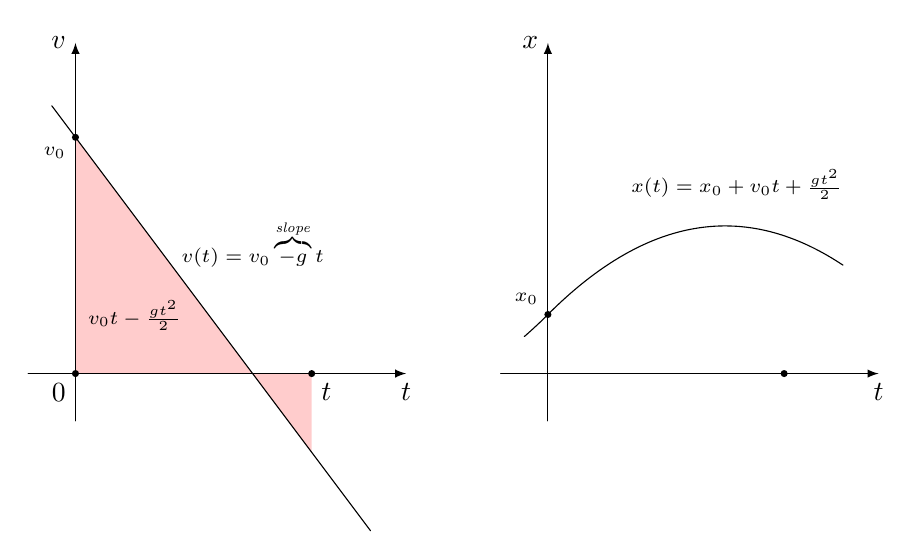
\begin{tikzpicture}
    [line cap=round,line join=round,x=2cm,y=2cm, scale=1.5, decoration={brace,amplitude=2pt}]
%main layer
%creating the ticks and xy-axis nodes
%some function
\fill[fill=red!20] (0,0) -- plot [domain=0:1] (\x,{-\x/0.75+1}) -- plot [domain=01: 0.0] (\x,0) -- cycle;

 \draw[smooth,samples=100,domain=-0.1:1.25]
                                 plot(\x,{-\x/0.75+1});
 
  %\draw [darkgray,ultra thin] (0,0.479)-- (0.25,0.479);
  %\draw [darkgray,ultra thin] (0,0.938)-- (0.75,0.938);
 % \draw [darkgray,ultra thin] (0.25,0.479)-- (0.25,0.0);
  %\draw [darkgray,ultra thin] (0.75,0.938)-- (0.75,0);
%creating the curly braces with decorate
 
%  \draw [decorate,color=black!80!black] (0.25,0.0)--(0.75,0.0)
   %node [midway,anchor=north,inner sep=1pt, outer sep=1pt]{\small$\Delta x$};
    \fill[black] (0,0) circle (0.3mm) node [anchor=north east,scale=1] {$ 0$};
     \fill[black] (1,0) circle (0.3mm) node [anchor=north west ,scale=1] {$t$};
      \fill[black] (0,1) circle (0.3mm) node [anchor=north east,scale=1] {\scriptsize$ v_0$};

  \draw[-latex,color=black,thin] (-0.2,0) -- (1.4,0) node [anchor=north ,scale=1] {$t$};
   \draw[-latex,color=black,thin] (0,-0.2) -- (0,1.4)node [anchor=east ,scale=1] {$v$};
     \draw (0.75,0.55) node [anchor=center ,scale=1] {\scriptsize$v(t)=v_0\overbrace{-g}^{\textit{slope}}t$};
        \draw (0.25,0.35) node [anchor=north ,scale=1] {\scriptsize$v_0t-\frac{gt^2}{2}$};
        
        
        \begin{scope}[shift={(2,0)}]
 \draw[smooth,samples=100,domain=-0.1:1.25]
                                 plot(\x,{0.25-\x^2/1.5+\x});
      \fill[black] (0,0.25) circle (0.3mm) node [anchor=south east,scale=1] {\scriptsize$ x_0$};

  \draw[-latex,color=black,thin] (-0.2,0) -- (1.4,0) node [anchor=north ,scale=1] {$t$};
   \draw[-latex,color=black,thin] (0,-0.2) -- (0,1.4)node [anchor=east ,scale=1] {$x$};
     \draw (0.8,0.8) node [anchor=center ,scale=1] {\scriptsize$x(t)=x_0+v_0t+\frac{gt^2}{2}$};
     \fill[black] (1,0) circle (0.3mm) node [anchor=north west ,scale=1] {$$};
\end{scope}
 \end{tikzpicture}
$$
\newpage
 \section{2-D Constant Velocity}
 \marginnote[50pt]{In two dimensions position, velocity and acceleration are represented by 2D vectors.  Acceleration is zero so velocity does not change from its initial state $\overrightarrow{v}_0$.}
 
 \marginnote[300pt]{The velocity vector does not change.  The position vector propagates linearly in the $\hat{v}$ direction from the initial position $\overrightarrow{r}_0$..}
 \vspace{1cm}
 $$\overrightarrow{a}=0$$
 \vspace{1cm}
$$v_x=v_{0x}$$
$$v_y=v_{0y}$$
$$\overrightarrow{v}=\left(\begin{array}{c} v_x \\ v_y \end{array}\right)=\left(\begin{array}{c} v_{0x} \\ v_{0y} \end{array}\right)=\overrightarrow{v}_0$$
\vspace{1cm}
$$x=x_0+v_{0x}t$$
$$y=y_0+v_{0y}t$$

$$\overrightarrow{r}=\left(\begin{array}{c} x \\ y \end{array}\right)=\left(\begin{array}{c} x_0+v_{0x}t \\ y_0+v_{0y}t \end{array}\right)=\left(\begin{array}{c} x_0 \\ y_0 \end{array}\right)+\left(\begin{array}{c}v_{0x} \\ v_{0y} \end{array}\right)t=\overrightarrow{r}_0+\overrightarrow{v}_0t$$

\vspace{1cm}$$
 \begin{tikzpicture}
    [line cap=round,line join=round,x=2cm,y=2cm, scale=1.5, decoration={brace,amplitude=2pt}]
%main layer
%creating the ticks and xy-axis nodes
%some function
%\fill[fill=red!20] (0,0) -- plot [domain=0:1] (\x,{-\x/0.75+1}) -- plot [domain=01: 0.0] (\x,0) -- cycle;

% \draw[smooth,samples=1000,domain=-0.1:1.25]
     %                            plot(\x,{-\x/0.75+1});
 
  %\draw [darkgray,ultra thin] (0,0.479)-- (0.25,0.479);
  %\draw [darkgray,ultra thin] (0,0.938)-- (0.75,0.938);
 % \draw [darkgray,ultra thin] (0.25,0.479)-- (0.25,0.0);
  %\draw [darkgray,ultra thin] (0.75,0.938)-- (0.75,0);
%creating the curly braces with decorate
 
%  \draw [decorate,color=black!80!black] (0.25,0.0)--(0.75,0.0)
   %node [midway,anchor=north,inner sep=1pt, outer sep=1pt]{\small$\Delta x$};
   % \fill[black] (0,0) circle (0.3mm) node [anchor=north east,scale=1] {$ 0$};
   %  \fill[black] (1,0) circle (0.3mm) node [anchor=north west ,scale=1] {$t$};
      \fill[black] (0.6,0.3) circle (0.3mm) node [anchor=south east,scale=1] {\scriptsize$\overrightarrow{v}=\overrightarrow{v}_0$};

 % \draw[-latex,color=black,thin] (-0.1,0.15) -- (1.2,0.8);
   \draw[-latex,color=black,thin] (0,-0.2) -- (0,1.4)node [anchor=east ,scale=1] {$v_y$};
    \draw[-stealth,color=black,thin] (-0.2,0) -- (1.4,0) node [anchor=north ,scale=1] {$v_x$};
    % \draw (0.75,0.8) node [anchor=center ,scale=1] {\scriptsize$\overrightarrow{r}(t)=\overrightarrow{r}_0+\overrightarrow{v}t$};
      %  \draw (0.25,0.35) node [anchor=north ,scale=1] {\scriptsize$v_0t-\frac{gt^2}{2}$};
        
        

 \end{tikzpicture}
 \hspace{1cm}
 \begin{tikzpicture}
    [line cap=round,line join=round,x=2cm,y=2cm, scale=1.5, decoration={brace,amplitude=2pt}]
%main layer
%creating the ticks and xy-axis nodes
%some function
%\fill[fill=red!20] (0,0) -- plot [domain=0:1] (\x,{-\x/0.75+1}) -- plot [domain=01: 0.0] (\x,0) -- cycle;

% \draw[smooth,samples=1000,domain=-0.1:1.25]
     %                            plot(\x,{-\x/0.75+1});
 
  %\draw [darkgray,ultra thin] (0,0.479)-- (0.25,0.479);
  %\draw [darkgray,ultra thin] (0,0.938)-- (0.75,0.938);
 % \draw [darkgray,ultra thin] (0.25,0.479)-- (0.25,0.0);
  %\draw [darkgray,ultra thin] (0.75,0.938)-- (0.75,0);
%creating the curly braces with decorate
 
%  \draw [decorate,color=black!80!black] (0.25,0.0)--(0.75,0.0)
   %node [midway,anchor=north,inner sep=1pt, outer sep=1pt]{\small$\Delta x$};
   % \fill[black] (0,0) circle (0.3mm) node [anchor=north east,scale=1] {$ 0$};
   %  \fill[black] (1,0) circle (0.3mm) node [anchor=north west ,scale=1] {$t$};
      \fill[black] (0.3,0.35) circle (0.3mm) node [anchor=south east,scale=1] {\scriptsize$\overrightarrow{r}_0$};

  \draw[-latex,color=black,thin] (-0.1,0.15) -- (1.2,0.8);
   \draw[-latex,color=black,thin] (0,-0.2) -- (0,1.4)node [anchor=east ,scale=1] {$y$};
    \draw[-stealth,color=black,thin] (-0.2,0) -- (1.4,0) node [anchor=north ,scale=1] {$x$};
     \draw (0.75,0.8) node [anchor=center ,scale=1] {\scriptsize$\overrightarrow{r}(t)=\overrightarrow{r}_0+\overrightarrow{v}_0t$};
      %  \draw (0.25,0.35) node [anchor=north ,scale=1] {\scriptsize$v_0t-\frac{gt^2}{2}$};
        
        

 \end{tikzpicture}
$$
\vspace{1cm}
\newpage

\section{Projectile Motion}
\marginnote[0pt]{In projectile motion there is no acceleration in the horizontal direction and constant acceleration in the vertical direction.  Under these conditions the initial position and velocity completely determines the evolution of the system.  Take x and y as the horizontal and vertical components respectively.  In the $x$ direction there is no acceleration and constant velocity making $x(t)$ a linear function.  In the $y$ direction the acceleration is constant and velocity changing linearly as a function of time.  This makes $y(t)$ a parabolic function.  The trajectory is also a parabolic function.}
$$\overrightarrow{a}=-g\hat{y}=\left(\begin{array}{c} 0 \\ -g \end{array}\right)$$
$$v_x=v_{0x}$$
$$v_y=v_{0y}+a_yt=v_{0y}-gt$$
$$\overrightarrow{v}=\left(\begin{array}{c} v_x \\ v_y \end{array}\right)=\left(\begin{array}{c} v_{0x} \\ v_{0y}-gt \end{array}\right)=\left(\begin{array}{c} v_{0x} \\ v_{0y} \end{array}\right)+\left(\begin{array}{c}0 \\ -g \end{array}\right)t=\overrightarrow{v}_0+\overrightarrow{a}t$$
$$x=x_0+v_{0x}t$$
$$y=y_0+v_{0y}t-\frac{gt^2}{2}$$
$$\overrightarrow{r}=\left(\begin{array}{c} x \\ y \end{array}\right)=\left(\begin{array}{c} x_0+v_{0x}t \\ y_0+v_{0y}t -\frac{gt^2}{2}\end{array}\right)=\left(\begin{array}{c} x_0 \\ y_0 \end{array}\right)+\left(\begin{array}{c}v_{0x} \\ v_{0y} \end{array}\right)t+\left(\begin{array}{c} 0 \\ -g \end{array}\right)\frac{t^2}{2}=\overrightarrow{r}_0+\overrightarrow{v}_0t+\overrightarrow{a}\frac{t^2}{2}$$

$$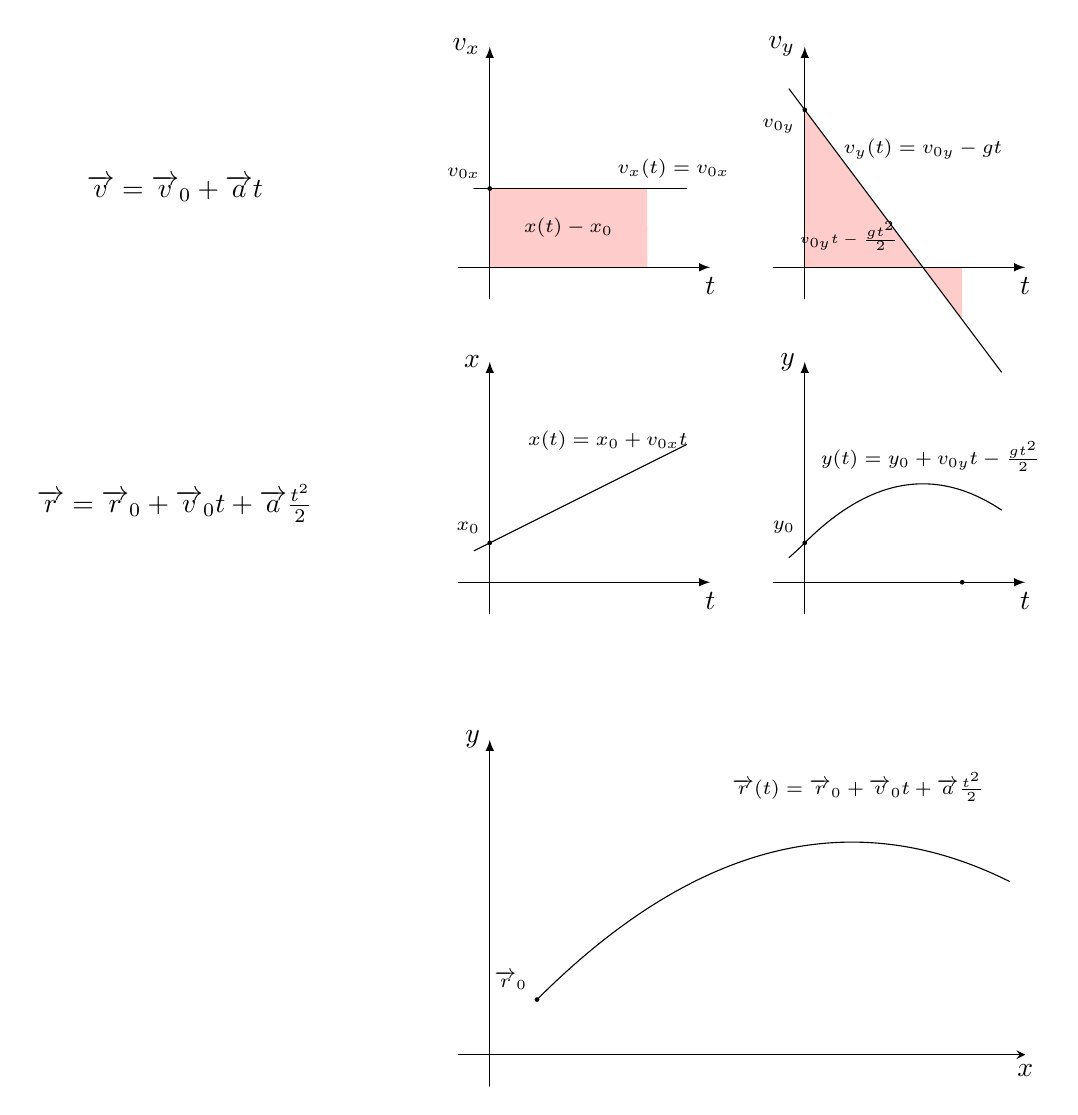
\begin{tikzpicture}
    [line cap=round,line join=round,x=2cm,y=2cm, scale=1, decoration={brace,amplitude=2pt}]
%main layer
%creating the ticks and xy-axis nodes
%some function
\fill[fill=red!20] (0,0) -- plot [domain=0:1] (\x,{-\x/0.75+1}) -- plot [domain=01: 0.0] (\x,0) -- cycle;

 \draw[smooth,samples=100,domain=-0.1:1.25]
                                 plot(\x,{-\x/0.75+1});
 
  %\draw [darkgray,ultra thin] (0,0.479)-- (0.25,0.479);
  %\draw [darkgray,ultra thin] (0,0.938)-- (0.75,0.938);
 % \draw [darkgray,ultra thin] (0.25,0.479)-- (0.25,0.0);
  %\draw [darkgray,ultra thin] (0.75,0.938)-- (0.75,0);
%creating the curly braces with decorate
 
%  \draw [decorate,color=black!80!black] (0.25,0.0)--(0.75,0.0)
   %node [midway,anchor=north,inner sep=1pt, outer sep=1pt]{\small$\Delta x$};
    %\fill[black] (0,0) circle (0.3mm) node [anchor=north east,scale=1] {$ 0$};
    % \fill[black] (1,0) circle (0.3mm) node [anchor=north west ,scale=1] {$t$};
      \fill[black] (0,1) circle (0.3mm) node [anchor=north east,scale=1] {\scriptsize$ v_{0y}$};

  \draw[-latex,color=black,thin] (-0.2,0) -- (1.4,0) node [anchor=north ,scale=1] {$t$};
   \draw[-latex,color=black,thin] (0,-0.2) -- (0,1.4)node [anchor=east ,scale=1] {$v_y$};
     \draw (0.75,0.75) node [anchor=center ,scale=1] {\scriptsize$v_y(t)=v_{0y}-gt$};
        \draw (0.28,0.35) node [anchor=north ,scale=1] {\tiny$v_{0y}t-\frac{gt^2}{2}$};
        
        
        \begin{scope}[shift={(0,-2)}]
 \draw[smooth,samples=100,domain=-0.1:1.25]
                                 plot(\x,{0.25-\x^2/1.5+\x});
      \fill[black] (0,0.25) circle (0.3mm) node [anchor=south east,scale=1] {\scriptsize$ y_0$};

  \draw[-latex,color=black,thin] (-0.2,0) -- (1.4,0) node [anchor=north ,scale=1] {$t$};
   \draw[-latex,color=black,thin] (0,-0.2) -- (0,1.4)node [anchor=east ,scale=1] {$y$};
     \draw (0.8,0.8) node [anchor=center ,scale=1] {\scriptsize$y(t)=y_0+v_{0y}t-\frac{gt^2}{2}$};
     \fill[black] (1,0) circle (0.3mm) node [anchor=north west ,scale=1] {$$};
\end{scope}

\begin{scope}[shift={(-2,0)}]
\fill[fill=red!20] (0,0) -- plot [domain=0:1] (\x,0.5) -- plot [domain=1: 0.0] (\x,0) -- cycle;

 \draw[smooth,samples=100,domain=-0.1:1.25]
                                 plot(\x,0.5);

  %  \fill[black] (0,0) circle (0.3mm) node [anchor=north east,scale=1] {$ 0$};
    % \fill[black] (0.75,0) circle (0.3mm) node [anchor=north ,scale=1] {$t$};
      \fill[black] (0,0.5) circle (0.3mm) node [anchor=south east,scale=1] {\scriptsize$ v_{0x}$};

  \draw[-latex,color=black,thin] (-0.2,0) -- (1.4,0) node [anchor=north ,scale=1] {$t$};
   \draw[-latex,color=black,thin] (0,-0.2) -- (0,1.4)node [anchor=east ,scale=1] {$v_x$};
     \draw (0.75,0.5) node [anchor=south west ,scale=1] {\scriptsize$v_x(t)=v_{0x}$};
        \draw (0.5,0.25) node [anchor=center ,scale=1] {\scriptsize$x(t)-x_0$};
\end{scope}

\begin{scope}[shift={(-2,-2)}]
 \draw[smooth,samples=100,domain=-0.1:1.25]
                                 plot(\x,{0.25+\x/2});

      \fill[black] (0,0.25) circle (0.3mm) node [anchor=south east,scale=1] {\scriptsize$ x_0$};

  \draw[-latex,color=black,thin] (-0.2,0) -- (1.4,0) node [anchor=north ,scale=1] {$t$};
   \draw[-latex,color=black,thin] (0,-0.2) -- (0,1.4)node [anchor=east ,scale=1] {$x$};
     \draw (0.75,0.9) node [anchor=center ,scale=1] {\scriptsize$x(t)=x_0+v_{0x}t$};
\end{scope}

\begin{scope}[shift={(-2,-5)}]
      \fill[black] (0.3,0.35) circle (0.3mm) node [anchor=south east,scale=1] {\scriptsize$\overrightarrow{r}_0$};

%  \draw[-latex,color=black,thin] (-0.1,0.15) -- (1.2,0.8);
 \draw[smooth,samples=100,domain=-0:3]
                                 plot({0.3+\x},{0.35-\x^2/4+\x});
   \draw[-latex,color=black,thin] (0,-0.2) -- (0,2)node [anchor=east ,scale=1] {$y$};
    \draw[-stealth,color=black,thin] (-0.2,0) -- (3.4,0) node [anchor=north ,scale=1] {$x$};
     \draw (3.2,1.7) node [anchor=east ,scale=1] {\scriptsize$\overrightarrow{r}(t)=\overrightarrow{r}_0+\overrightarrow{v}_0t+\overrightarrow{a}\frac{t^2}{2}$};
      %  \draw (0.25,0.35) node [anchor=north ,scale=1] {\scriptsize$v_0t-\frac{gt^2}{2}$};
\end{scope}
 \draw (-4,0.5) node [anchor=center ,scale=1] {$\overrightarrow{v}=\overrightarrow{v}_0+\overrightarrow{a}t$};
   \draw (-4,-1.5) node [anchor=center ,scale=1] {$\overrightarrow{r}=\overrightarrow{r}_0+\overrightarrow{v}_0t+\overrightarrow{a}\frac{t^2}{2}$};

 \end{tikzpicture}
$$
\newpage
\subsection{Components of Initial Velocity}
\marginnote[0pt]{In the physics game initial velocity is often parameterized in terms of the launch angle and initial speed.  Trigonometry is used to get the x and y components of the initial velocity.}
$$
 \begin{tikzpicture}
    [line cap=round,line join=round,x=2cm,y=2cm, scale=1.5, decoration={brace,amplitude=2pt}]

\draw (-0.2,0.7) node [anchor=east,color=black]{$\overrightarrow{v}_0=v_{0x}\hat{x}+v_{0y}\hat{y}=\left(\begin{array}{c} v_{0x} \\ v_{0y}\end{array}\right)=\left(\begin{array}{c} v_0\ \cos \theta\\ v_0\ \sin \theta\end{array}\right)=v_0\left(\begin{array}{c} \cos \theta\\  \sin \theta\end{array}\right)$};
      \fill[black] (0.9,0.45) circle (0.3mm) node [anchor=south east,scale=1] {\scriptsize$\overrightarrow{v}_0$};

  \draw[-latex,color=black,thin] (0,0) -- (0.9,0.45);
   \draw[-latex,color=black,thin] (0,-0.2) -- (0,1.4)node [anchor=east ,scale=1] {$v_y$};
    \draw[-latex,color=black,thin] (-0.2,0) -- (1.4,0) node [anchor=north ,scale=1] {$v_x$};
    \draw (0.55,0) arc (0:26.57:0.55) ;
\draw (0.3,0.0) node [anchor=south west,color=black]{\scriptsize$\theta$};
\draw[dashed, color=red] (0.9,0) -- (0.9,0.45) node[midway,anchor=west ,scale=1,color=black] {\scriptsize$v_{0y}$};
\draw[dashed, color=red] (0,0.45) -- (0.9,0.45) node[midway,anchor=south ,scale=1,color=black] {\scriptsize$v_{0x}$};
    % \draw (0.75,0.8) node [anchor=center ,scale=1] {\scriptsize$\overrightarrow{r}(t)=\overrightarrow{r}_0+\overrightarrow{v}t$};
      %  \draw (0.25,0.35) node [anchor=north ,scale=1] {\scriptsize$v_0t-\frac{gt^2}{2}$};
 \end{tikzpicture}
 $$
 
 \section{Relative Position and Velocity}
\vspace{1cm}
\marginnote[0pt]{Relative position of "b" according to "a" is the position of "b" that would be measured if the origin of coordinates were positioned at "a".  Relative velocity of "b" according to "a" is the velocity of "b" that would be measured if the origin of coordinates were moving at the velocity of "a".}


$$
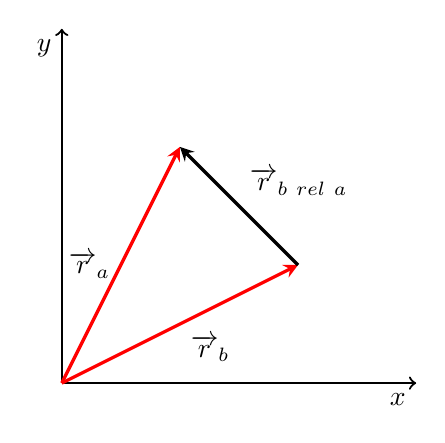
\begin{tikzpicture}[scale=1.5]


\draw[thick,->] (0,0,0) -- (3,0,0) node[anchor=north east]{$x$};
\draw[thick,->] (0,0,0) -- (0,3,0) node[anchor=north east]{$y$};


%draw a vector from origin to point (P) 
\draw[-stealth,very thick,color=red] (0,0) -- (1,2) node[midway,anchor=east,color=black]{$ \overrightarrow{r}_a$};
\draw[-stealth,very thick,color=red] (0,0) -- (2,1) node[midway, anchor=north west ,color=black]{$\overrightarrow{r}_b$};
\draw[-stealth,very thick,color=black] (2,1) -- (1,2) node[midway, anchor=south west ,color=black]{$\overrightarrow{r}_{b\ rel\ a}$};
%\draw[-stealth,very thick,color=black] (1,2) -- (1.2,2.4) node[anchor=south,color=black]{$\hat{r}$};
%\draw[-stealth,very thick,color=black] (1,2) -- (0.6,2.2) node[anchor=east,color=black]{$\hat{\theta}$};


%draw projection on xy plane, and a connecting line
%\draw (0.75,0) arc (0:60:0.75) ;
%\draw (0.25,0.1) node [anchor=south west,color=black]{$\theta$};



\end{tikzpicture}
$$

\vspace{1cm}

\noindent For non-relativistic speeds we assume velocities much slower than the speed of light and can calculate as follows.

$$\overrightarrow{r}_{b\ rel\ a}=\overrightarrow{r}_{a}-\overrightarrow{r}_{b}$$
\vspace{1cm}
$$\overrightarrow{v}_{b\ rel\ a}=\overrightarrow{v}_{a}-\overrightarrow{v}_{b}$$






\chapter{Rotational Kinematics}
\begin{marginfigure}%
  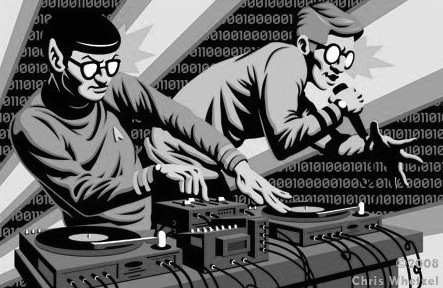
\includegraphics[width=\linewidth]{nerd5.jpg}
  \caption{Turntablism is largely an art of rotational kinematics}
  \label{fig:marginfig}
\end{marginfigure}
\textit{Joy is the mainspring... in Nature's calm rotation.}  \\
\noindent\textbf{-Friedrich Schiller}
\vspace{1cm}
\section{Pure Rotation}

\begin{margintable}[50pt]
\begin{center}
\footnotesize
\begin{tabular}{lllll}
\toprule
 Translation         & Rotation                                                    \\
\midrule
  Position $(x)$  & Angle $(\theta)$       \\
  Velocity $(v)$ & Angular Velocity$(\omega)$           \\
   Acceleration $(a)$  & Angular Acceleration$(\alpha)$                        \\
\bottomrule
\end{tabular}
\end{center}
  \caption{Translational and rotational analogues}
  \label{tab:font-sizes}
\end{margintable}

$$
\begin{tikzpicture}
    [line cap=round,line join=round,x=2cm,y=2cm, scale=1, decoration={brace,amplitude=2pt}]


%\draw[->, xshift=0cm]  (120:2.4cm) arc (120:170:2.4) node[below] {$\omega$};
    \draw[color=gray,thin] (-1.6,0) -- (1.6,0)  ;
   \draw[color=gray,thin] (0,-1.6) -- (0,1.6);
  
 
  \draw[thick,red,->] ([shift=(105:2cm)]0,0) arc (105:150:2cm) node [below, black] {$\omega$};
  \draw (0,0) circle (3cm);
  \draw[fill=green, thick ] ([shift=(0:1.5cm)]0,0) arc (0:30:1.5cm) -- (0,0) -- cycle;
   \draw[fill=green, thick ] ([shift=(30:1.5cm)]0,0) arc (30:45:1.5cm) -- (0,0) -- cycle;
   \draw (0.5,0) node [anchor=south ,scale=1] {$\theta$};
  
    %  \fill[black] (0,0.1) circle (0.3mm) node [anchor=south east,scale=1] {\scriptsize$ \theta(0)$};

    % \draw (0.6,0.8) node [anchor=south west ,scale=1] {$\theta(t)$};
    
 \end{tikzpicture}
$$

\subsubsection{Angular Velocity}
\marginnote[0pt]{The angular velocity is the rate of change of the angle value.  The lowercase Greek letter omega is used to represent it as an algebraic variable.}
$$\omega=\lim_{\Delta \rightarrow 0}\frac{\Delta \theta}{\Delta t}$$
$$\bar{\omega}=\frac{\Delta \theta}{\Delta t}=\frac{2\pi \theta}{T}$$

\subsubsection{Angular Acceleration}
\marginnote[0pt]{Angular acceleration is the time rate of change of the angular velocity.  The lowercase Greek letter alpha is used to represent it as an algebraic variable.}
$$\alpha=\lim_{\Delta \rightarrow 0}\frac{\Delta \omega}{\Delta t}$$

\subsection{Kinematics Equations for Angular Motion}


\subsubsection{Constant Angular Velocity}
\marginnote[0pt]{Under zero acceleration the angular velocity is constant.  The angle is a linear function of time with a slope equal to the angular velocity.}
$$\alpha=0$$
$$\omega=\omega_0$$
$$\theta=\theta_0+\omega t$$

\subsubsection{Constant Angular Acceleration}
\marginnote[0pt]{Under constant acceleration the angular velocity is a linear function of time with a slope equal to the angular acceleration.  The angle is a quadratic function of time.  The angular velocity may also be parameterized as a function of angle.}
$$\omega=\omega_0+\alpha t$$
$$\bar{\omega}=\frac{\omega_0+\omega}{2}$$
$$\theta=\theta_0+\omega_0t+\frac{\alpha t^2}{2}=\theta_0+\bar{\omega}t$$
$$\omega^2-\omega_0^2=2\alpha(\theta-\theta_0)$$


\subsubsection{Variable Angular Acceleration}
\marginnote[70pt]{$$\Delta \omega=\text{Area under }\alpha(t)$$ }
$$
\begin{tikzpicture}
    [line cap=round,line join=round,x=2cm,y=2cm, scale=1, decoration={brace,amplitude=2pt}]

\fill[fill=red!20] (0,0) -- plot [domain=0:.5] (\x,{1-\x}) -- plot [domain=0.5: 0.0] (\x,0) -- cycle;

 \draw[smooth,samples=100,domain=-0.1:1.25]
                                 plot(\x,{1-\x});

    \fill[black] (0,0) circle (0.3mm) node [anchor=north east,scale=1] {$ 0$};
     \fill[black] (0.5,0) circle (0.3mm) node [anchor=north ,scale=1] {$t$};

  \draw[-latex,color=black,thin] (-0.2,0) -- (1.4,0) node [anchor=north ,scale=1] {$t$};
   \draw[-latex,color=black,thin] (0,-0.2) -- (0,1.4)node [anchor=east ,scale=1] {$\alpha$};
    \draw (0.6,0.6) node [anchor=south west ,scale=1] {$\alpha(t)$};
        \draw (0.25,0.3) node [anchor=center ,scale=1] {\tiny$\omega(t)-\omega(0)$};
        
 \end{tikzpicture}
$$
\marginnote[70pt]{$$\omega(t)=\omega(0)+\text{Area}(\alpha(t))$$
$$\Delta \theta=\text{Area under }\omega(t)$$ }
$$
\begin{tikzpicture}
    [line cap=round,line join=round,x=2cm,y=2cm, scale=1, decoration={brace,amplitude=2pt}]

\fill[fill=red!20] (0,0) -- plot [domain=0:.5] (\x,{-\x^2/2+\x+0.25}) -- plot [domain=0.5: 0.0] (\x,0) -- cycle;

 \draw[smooth,samples=100,domain=-0.1:1.25]
                                 plot(\x,{-\x^2/2+\x+0.25});

    \fill[black] (0,0) circle (0.3mm) node [anchor=north east,scale=1] {$ 0$};
     \fill[black] (0.5,0) circle (0.3mm) node [anchor=north ,scale=1] {$t$};
      \fill[black] (0,0.25) circle (0.3mm) node [anchor=south east,scale=1] {\scriptsize$ \omega(0)$};

  \draw[-latex,color=black,thin] (-0.2,0) -- (1.4,0) node [anchor=north ,scale=1] {$t$};
   \draw[-latex,color=black,thin] (0,-0.2) -- (0,1.4)node [anchor=east ,scale=1] {$\omega$};
     \draw (0.6,0.8) node [anchor=south west ,scale=1] {$\omega(t)$};
        \draw (0.25,0.25) node [anchor=north ,scale=1] {\tiny$\theta(t)-\theta(0)$};
        
 \end{tikzpicture}
$$
\marginnote[70pt]{$$\theta(t)=\theta(0)+\text{Area}(\omega(t))$$ }
$$
\begin{tikzpicture}
    [line cap=round,line join=round,x=2cm,y=2cm, scale=1, decoration={brace,amplitude=2pt}]


 \draw[smooth,samples=100,domain=-0.1:1.25]
                                 plot(\x,{-\x^3/6+\x^2/2+\x/4+0.1});
  
      \fill[black] (0,0.1) circle (0.3mm) node [anchor=south east,scale=1] {\scriptsize$ \theta(0)$};
  \draw[-latex,color=black,thin] (-0.2,0) -- (1.4,0) node [anchor=north ,scale=1] {$t$};
   \draw[-latex,color=black,thin] (0,-0.2) -- (0,1.4)node [anchor=east ,scale=1] {$x$};
     \draw (0.6,0.8) node [anchor=south west ,scale=1] {$\theta(t)$};
    
 \end{tikzpicture}
$$

\newpage
\section{Angular and Radial Motion in Polar Coordinates}
\begin{figure}
$$
\begin{tikzpicture}[scale=1.5]


\draw[thick,->] (0,0,0) -- (3,0,0) node[anchor=north east]{$x$};
\draw[thick,->] (0,0,0) -- (0,3,0) node[anchor=north east]{$y$};


%draw a vector from origin to point (P) 
\draw[-stealth,very thick,color=red] (0,0) -- (1,2) node[anchor=south west,color=black]{$ $};
\draw[color=red] (0,0) -- (0.5,1) node[anchor=west ,color=black]{$\overrightarrow{r}$};
\draw[-stealth,very thick,color=black] (1,2) -- (1.2,2.4) node[anchor=south,color=black]{$\hat{r}$};
\draw[-stealth,very thick,color=black] (1,2) -- (0.6,2.2) node[anchor=east,color=black]{$\hat{\theta}$};


%draw projection on xy plane, and a connecting line
\draw (0.75,0) arc (0:60:0.75) ;
\draw (0.25,0.1) node [anchor=south west,color=black]{$\theta$};



\end{tikzpicture}
$$
 \caption{Position of a particle in polar coordintes}
  \label{fig:marginfig}
\end{figure}

\newthought{The unit vector in the radial direction} is determined by normalizing the position vector.  This is done by dividing the position vector by its magnitude.  
$$\hat{r}=\frac{\overrightarrow{r}}{r}=\frac{x\hat{x}+y\hat{y}}{\sqrt{x^2+y^2}}=\frac{r\cos \theta\hat{x}+r\sin \theta\hat{y}}{\sqrt{(r\cos \theta)^2+(r\sin \theta)^2}}=\cos \theta\hat{x}+\sin \theta\hat{y}=\left(\begin{array}{c} \cos \theta\\  \sin \theta\end{array}\right)$$
\noindent Perpendicular to the radial unit vector is the unit angular vector.  It points in the direction of increasing angle.

$$\hat{\theta}=-\sin \theta \hat{x}+\cos \theta\hat{y}=\left(\begin{array}{c}-\sin \theta\\  \cos \theta\end{array}\right)$$

\noindent The two unit vectors are orthogonal and together provide a handy coordinate system well suited for rotating systems.
$$\hat{r}\cdot{\hat{\theta}}=0$$

\subsection{Arc Length}
\marginnote[0pt]{For a fixed radius the arc length of a curve is the product of the radius and the angular change.  Angle is measured in radians.}
$$\Delta S= r \Delta \theta$$

\vspace{1cm}

\subsection{Period}
\marginnote[0pt]{The characteristic time for one whole rotation to occur is called the period.}
$$\text{time for a complete rotation}=T$$

\newpage
\subsection{Velocity}

\vspace{1cm}

\marginnote[0pt]{This figure shows change in position expressed in terms of polar components, in the radial direction and the angular (tangential) direction.}

\begin{center}
\begin{tabular}{cc}
\begin{minipage}{7cm}
\begin{tikzpicture}[scale=1.5]


\draw[thick,->] (0,0,0) -- (3,0,0) node[anchor=north east]{$x$};
\draw[thick,->] (0,0,0) -- (0,3,0) node[anchor=north east]{$y$};


%draw a vector from origin to point (P) 
\draw[-stealth,very thick,color=red] (0,0) -- (1,2) node[anchor=west,color=black, scale=0.7]{$\overrightarrow{r}(t) $};
\draw[-stealth,very thick,color=red] (0,0) -- (0.7,2.4)node[anchor=south,color=black, scale=0.7]{$\overrightarrow{r}(t+\Delta t) $};
%\draw[color=red] (0,0) -- (0.5,1) node[anchor=west ,color=black]{$\overrightarrow{r}(t)$};



%draw projection on xy plane, and a connecting line
\draw (0.75,0) arc (0:60:0.75) ;
\draw (0.25,0.1) node [anchor=south west,color=black]{$\theta$};
\draw (0.25,0.85) node [anchor=south west,color=black,scale=0.5]{$\Delta \theta$};
%\draw[-stealth,very thick,color=black] (1,2) -- (0.7,2.4) node[anchor=east,color=black, scale=0.7]{$ $};



\end{tikzpicture}
\end{minipage}
&
\begin{minipage}{7cm}

\begin{tikzpicture}[scale=1.5]


\draw[thick,->] (0,0,0) -- (3,0,0) node[anchor=north east]{$x$};
\draw[thick,->] (0,0,0) -- (0,3,0) node[anchor=north east]{$y$};


%draw a vector from origin to point (P) 
\draw[-stealth,very thick,color=red] (0,0) -- (1,2) node[anchor=south west,color=black]{$ $};
\draw[-stealth,very thick,color=red] (0,0) -- (1.1,2.2);
%\draw[color=red] (0,0) -- (0.5,1) node[anchor=west ,color=black]{$\overrightarrow{r}(t)$};
\draw[-stealth,very thick,color=black] (1,2) -- (1.1,2.2) node[anchor=west,color=black, scale=0.7]{$\overrightarrow{v}_r \Delta t$};
\draw[-stealth,very thick,color=black] (1,2) -- (0.6,2.2) node[anchor=east,color=black, scale=0.7]{$\overrightarrow{v}_t \Delta t$};
\draw[-stealth,very thick,color=black] (1,2) -- (0.7,2.4) node[anchor=east,color=black, scale=0.7]{$ $};


%draw projection on xy plane, and a connecting line
%\draw (0.75,0) arc (0:60:0.75) ;
%\draw (0.25,0.1) node [anchor=south west,color=black]{$\theta$};



\end{tikzpicture}



\end{minipage}
\end{tabular}
\end{center}
\vspace{1cm}


\subsubsection{Tangential Velocity}
\marginnote[0pt]{The angular velocity and radius are the two factors contributing to the tangential velocity. }
$$v_{tan}=r\omega$$
$$\overrightarrow{v}_{tan}=v_{tan}\hat{\theta}$$

\subsubsection{Radial Velocity}
\marginnote[0pt]{The radial velocity is the time rate of change of the radius.}
$$v_r=\lim_{\Delta \rightarrow 0}\frac{\Delta r}{\Delta t}$$
$$\overrightarrow{v}_{rad}=v_r\hat{r}$$
\subsubsection{Total Velocity}
\marginnote[0pt]{The total velocity is the vector sum of these two orthogonal components.}
$$\overrightarrow{v}=\lim_{\Delta \rightarrow 0}\frac{\Delta \overrightarrow{r}}{\Delta t}$$
$$\overrightarrow{v}=\underbrace{r\omega\hat{\theta}}_{\textit{tangential}}+\overbrace{v_r\hat{r}}^{\textit{radial}}$$

\vspace{1cm}


\begin{marginfigure}[70pt]%
  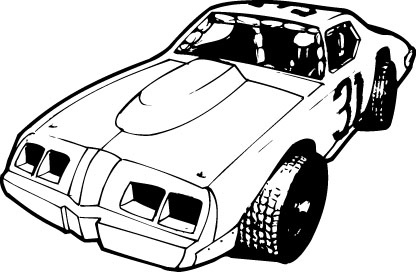
\includegraphics[width=\linewidth]{car.jpg}
  \caption{A rad car}
  \label{fig:marginfig}
\end{marginfigure}
\noindent Consider a car driving around a circular racetrack.  The magnitude of the tangential velocity determines how quickly the car circles the track.  The magnitude of the radial velocity determines how quickly the car changes lanes.  

\newpage

\subsection{Acceleration}

\vspace{1cm}

\subsubsection{Tangential Acceleration}
\marginnote[0pt]{The angular acceleration and radius are the two factors contributing to the tangential acceleration. }
$$a_{tan}=r\alpha$$
$$\overrightarrow{a}_{tan}=a_{tan}\hat{\theta}$$
\subsubsection{Centripetal Acceleration}
\marginnote[0pt]{Centripetal acceleration is the acceleration associated with circular motion.   }
$$a_{c}=r\omega^2=\frac{v^2_{tan}}{r}$$
$$\overrightarrow{a}_{c}=-a_{c}\hat{r}$$
\subsubsection{Coriolis Acceleration}
\marginnote[0pt]{The coriolis acceleration is strange.  It is dependent on the velocity in the tangential direction and the radial direction.    }
$$a_{C}=2v_r\omega=\frac{2v_r v_{tan}}{r}$$
$$\overrightarrow{a}_{C}=a_{C}\hat{\theta}$$
\subsubsection{Radial Acceleration}
\marginnote[0pt]{The radial acceleration is simply the time rate of change of the radial velocity.  }
$$a_r=\lim_{\Delta \rightarrow 0}\frac{\Delta v_r}{\Delta t}$$
$$\overrightarrow{a}_{rad}=a_r\hat{r}$$

\subsubsection{Total Acceleration}
\marginnote[0pt]{The total acceleration is the vector sum of these four components.  The centripetal and radial acceleration are in the radial direction.  The coriolis and tangential acceleration are in the tangential direction. }
$$\overrightarrow{a}=\lim_{\Delta \rightarrow 0}\frac{\Delta \overrightarrow{v}}{\Delta t}$$
$$\overrightarrow{a}=\underbrace{r\alpha\hat{\theta}}_{\textit{tangential}}-\overbrace{r\omega^2\hat{r}}^{\textit{centripetal}}+\underbrace{2v_r\omega\hat{\theta}}_{\textit{Coriolis}}+\overbrace{a_r\hat{r}}^{\textit{radial}}$$

\vspace{1cm}

\begin{fullwidth}
\newthought{The Coriolis effect} is a deflection of moving objects when the motion is described relative to a rotating reference frame. In a reference frame with clockwise rotation, the deflection is to the left of the motion of the object; in one with counter-clockwise rotation, the deflection is to the right. Although recognized previously by others, the mathematical expression for the Coriolis force appeared in an 1835 paper by French scientist Gaspard-Gustave Coriolis, in connection with the theory of water wheels.\\ \ \\

Italian scientists Giovanni Battista Riccioli and his assistant Francesco Maria Grimaldi described the effect in connection with artillery in the 1651 Almagestum Novum, writing that rotation of the Earth should cause a cannonball fired to the north to deflect to the east. The effect was described in the tidal equations of Pierre-Simon Laplace in 1778.
\end{fullwidth}

\newpage
\section{Circular Motion}
\marginnote[0pt]{In circular motion the radius is fixed.  There is no radial velocity.    }
\vspace{1cm}
$$v_r=0$$
\marginnote[0pt]{The angular motion may be variable over time with changing speed and acceleration of rotation.  }
$$\{\theta(t),\omega(t), \alpha(t)\}$$
\vspace{1cm}
\marginnote[0pt]{There is only tangental velocity.   }
$$\overrightarrow{v}=\underbrace{r\omega\hat{\theta}}_{\textit{tangential}}+\cancel{\overbrace{v_r\hat{r}}^{\textit{radial}}}=\underbrace{r\omega\hat{\theta}}_{\textit{tangential}}$$
\vspace{1cm}
\marginnote[0pt]{The acceleration has only two terms, the tangential and the centripetal.  The tangential is due to angular acceleration.  The centrifugal is due to the constrained circularity of the motion.}
$$\overrightarrow{a}=\underbrace{r\alpha\hat{\theta}}_{\textit{tangential}}-\overbrace{r\omega^2\hat{r}}^{\textit{centripetal}}+\cancel{\underbrace{2v_r\omega\hat{\theta}}_{\textit{Coriolis}}}+\cancel{\overbrace{a_r\hat{r}}^{\textit{radial}}}=\underbrace{r\alpha\hat{\theta}}_{\textit{tangential}}-\overbrace{r{\omega}^2\hat{r}}^{\textit{centripetal}}=r\alpha\hat{\theta}-\frac{v^2}{r}\hat{r}$$
\vspace{1cm}
\subsection{Circular Motion:  Constant Speed}
\marginnote[0pt]{For circular motion at constant angular velocity the tangential velocity is constant.  There is no angular acceleration therefore and there is no tangential acceleration.  }
\vspace{1cm}
$$\omega(t)=\omega$$
$$\alpha=0$$
$$\theta(t)=\omega t +\theta_0$$
\vspace{1cm}
$$\overrightarrow{v}=r\omega\hat{\theta}=v\hat{\theta}$$
\vspace{1cm}
\marginnote[0pt]{The acceleration is centripetal, towards the center.   }
$$\overrightarrow{a}=\cancel{\underbrace{r\alpha\hat{\theta}}_{\textit{tangential}}}-\overbrace{r{\omega}^2\hat{r}}^{\textit{centrifugal}}=-\frac{v^2}{r}\hat{r}$$


\chapter{Forces and Frames}
\begin{marginfigure}%
  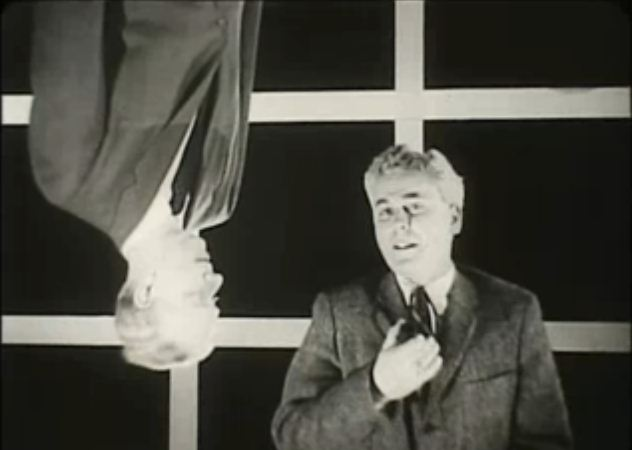
\includegraphics[width=\linewidth]{Frames.jpg}
  \caption{Frames of Reference is a 1960 educational film by Physical Sciences Study Committee.}
  \label{fig:marginfig}
\end{marginfigure}
\textit{The people... are the motive force.}  \\
\noindent\textbf{-  Mao Tse Tung}
\vspace{1cm}
\marginnote[30pt]{An inertial frame of reference is in a state of constant, rectilinear motion.  It is peaceful and non-accelerating.  Inertial is synonymous  with Newtonian and Galilean.  Newton's laws are only applicable in an inertial frame of reference.}


\section{Principia}
\textit{Philosophi\ae \ Naturalis Principia Mathematica}, Latin for "Mathematical Principles of Natural Philosophy", is often referred to simply as the Principia.  The work consists of three books by Sir Isaac Newton, in Latin, first published in 1687.  The Principia states Newton's laws of motion, forming the foundation of classical mechanics, also Newton's law of universal gravitation, and a mathematical derivation of Kepler's empirically derived laws of planetary motion. The Principia is justly regarded as one of the most important works in the history of science.

\begin{marginfigure}[30pt]%
  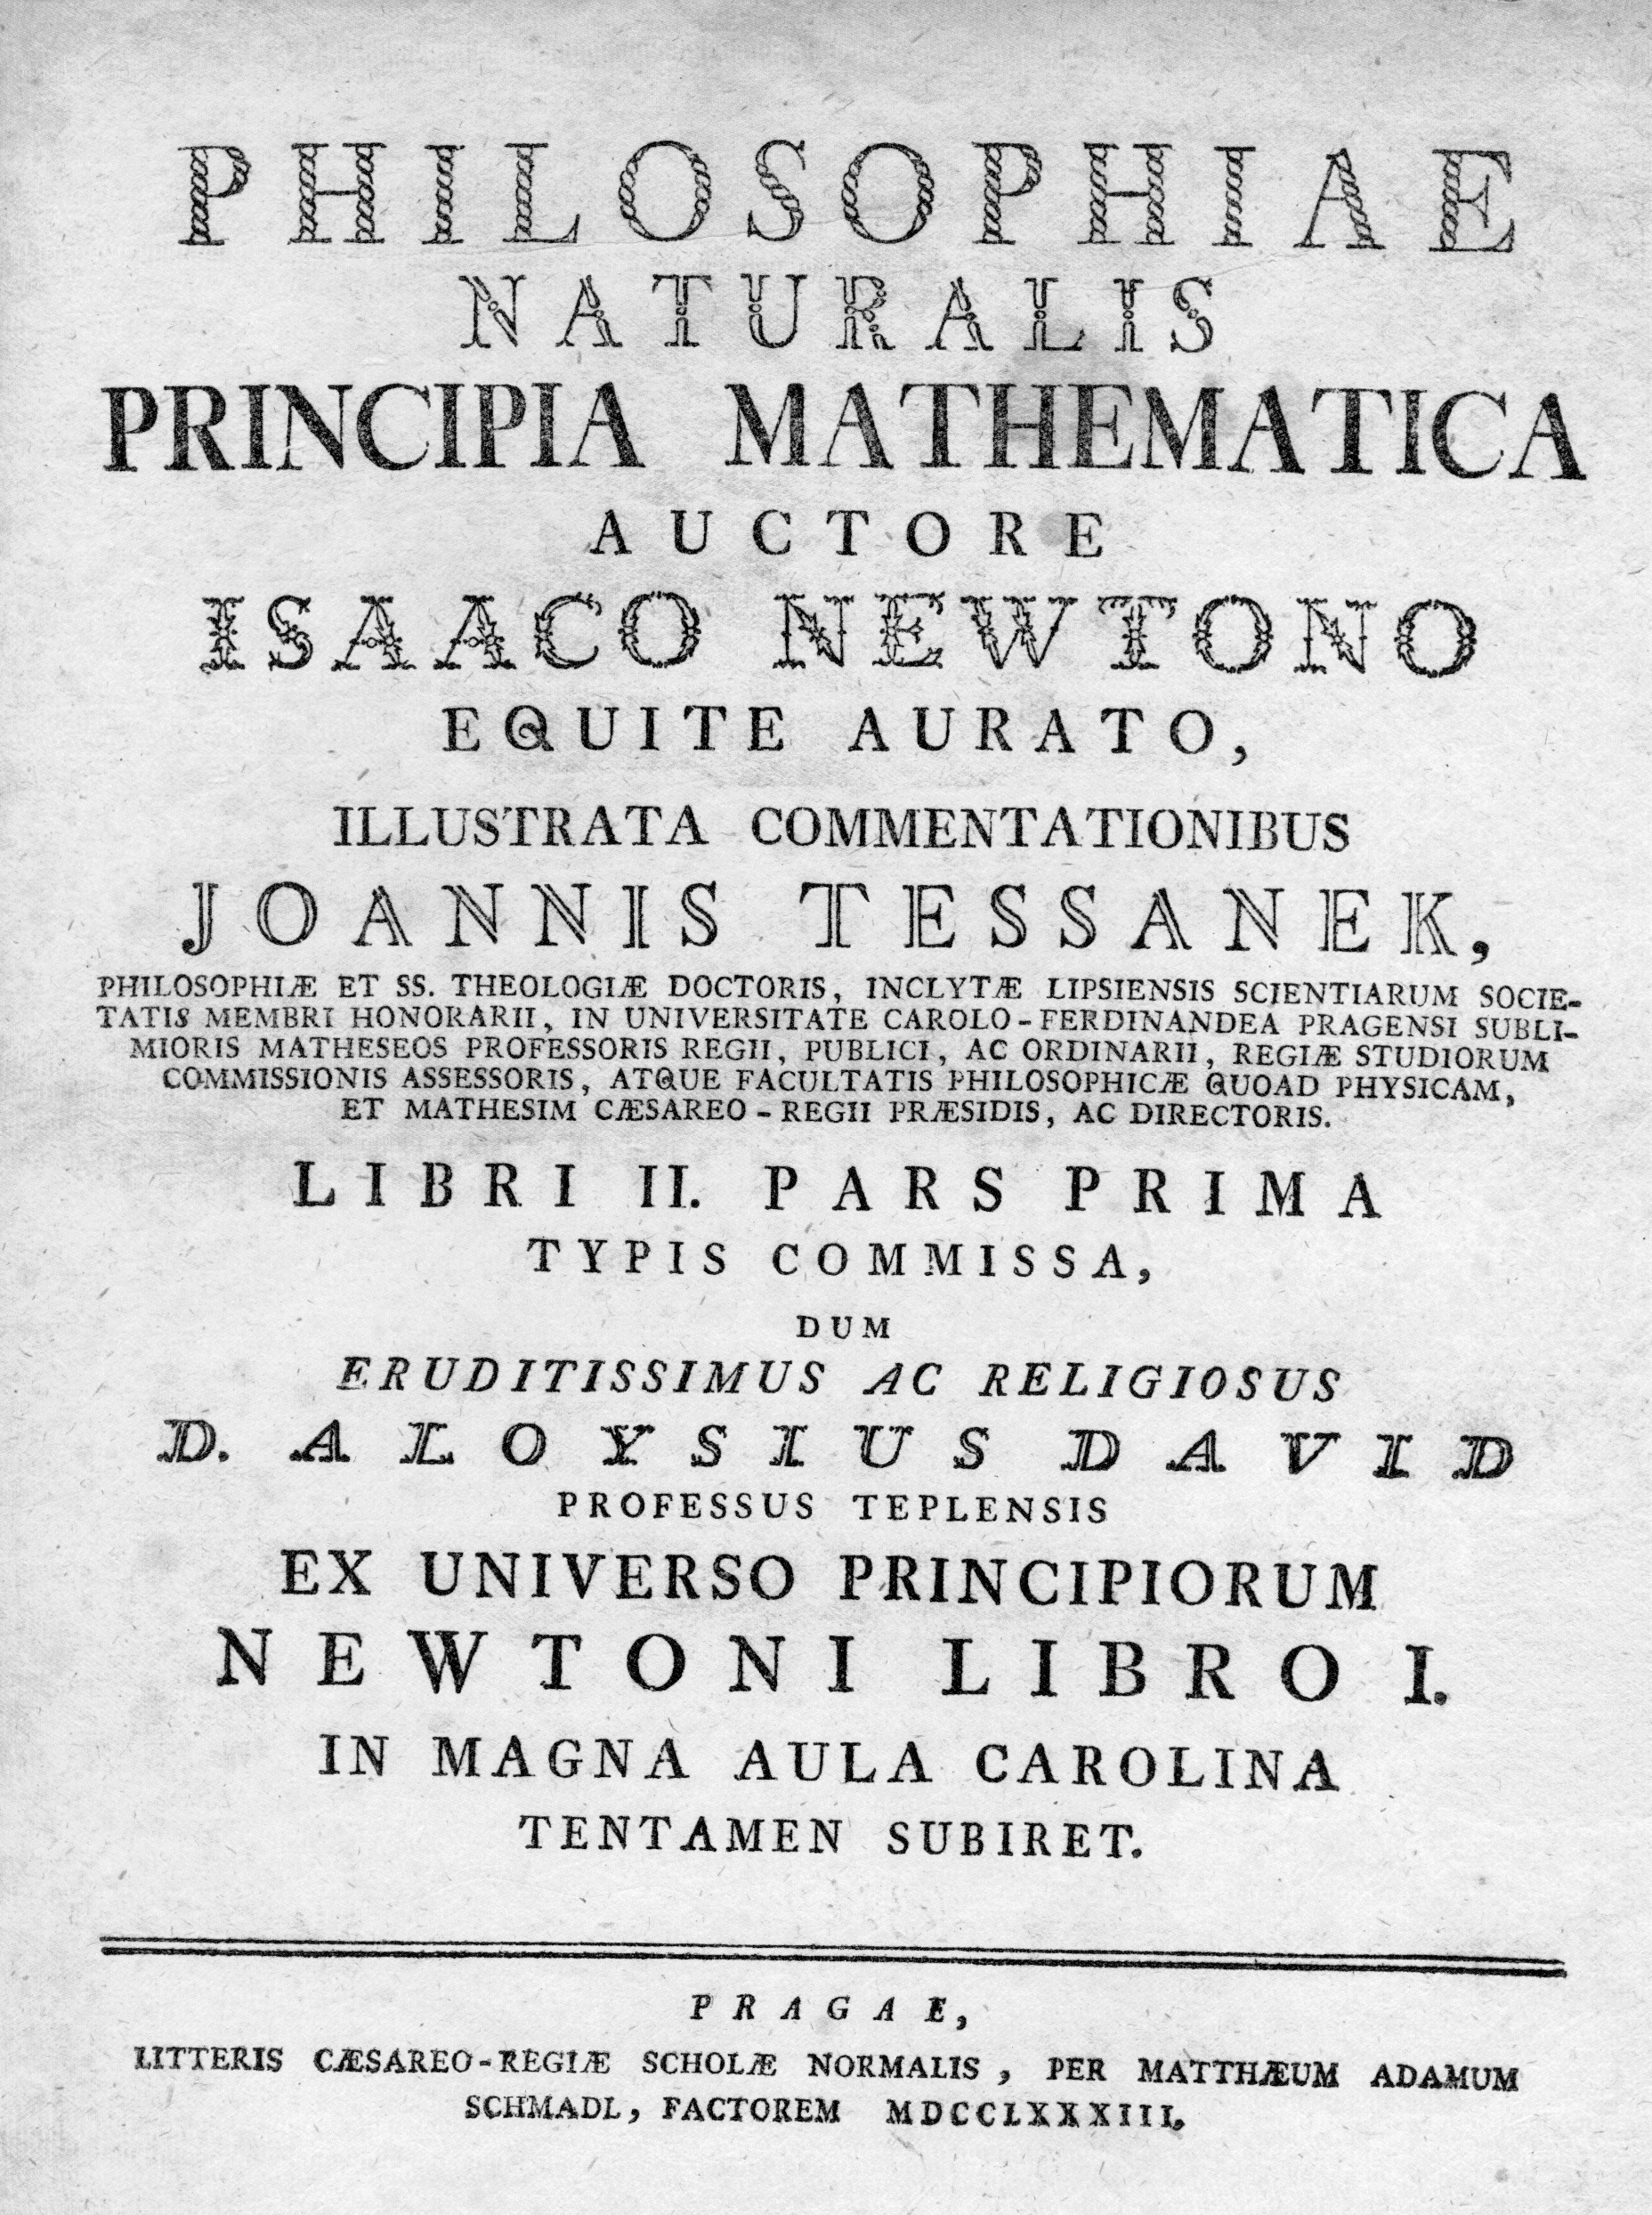
\includegraphics[width=\linewidth]{principia.jpg}
  \caption{The Principia}
  \label{fig:marginfig}
\end{marginfigure}


\section{Newton's First Law}


\textit{Every body perseveres in its state of being at rest or of moving uniformly straight forward, except insofar as it is compelled to change its state by forces impressed.} \textbf{\textit{- Principia}}


$$\sum \overrightarrow{F}=0\ \ \longrightarrow \ \ \overrightarrow{a}=0$$

\newthought{In an inertial frame}, an object at rest tends to stay at rest and an object in motion tends to stay in motion unless an external net force acts upon it.  Newton's first law is often called the Law of Inertia.

\newpage

 \marginnote[50pt]{
\textit{Inherent force of matter is the power of resisting by which every body, so far as it is able, perseveres in its state either of resting or of moving uniformly straight forward.}\\   \noindent\textbf{\textit{- Principia}}}
\subsection{Inertia}
\newthought{Inertia is the resistance} of any physical object to any change in its state of motion including changes to its speed and direction or the state of rest. It is the tendency of objects to keep moving in a straight line at constant velocity. The principle of inertia is one of the fundamental principles of classical physics that are used to describe the motion of objects and how they are affected by applied forces. Inertia comes from the Latin word, iners, meaning idle, sluggish. Inertia is one of the primary manifestations of mass.  Matter is the occupancy of mass over space therefore matter has inertia.
 


\begin{marginfigure}[110pt]%
  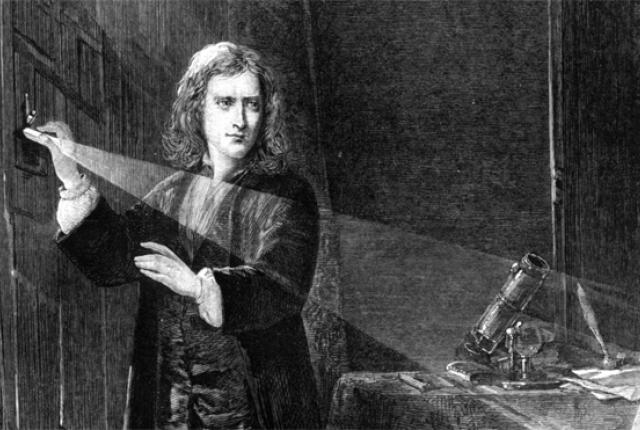
\includegraphics[width=\linewidth]{isaac-newton.jpg}
  \caption{Isaac Newton doing his thing}
  \label{fig:marginfig}
\end{marginfigure}
 
\subsection{  Space and Time Uniformity}
\begin{description}
  \item [Homogeneity] A homogeneous system has the same properties at every point; it is uniform without irregularities.  The laws of physics must be invariant (unchanging) to translations in space.  The location of the coordinate system does not change physics.
  \item [Isotropy]  A isotropic system has the same properties in all directions.  The laws of physics must be invariant to rotations in space.  The orientation of the coordinate system does not change physics.  
  \item [Time-Independence] A time-independent system has the same properties throughout time.  The laws of physics must be invariant to translations in time.  The start time of the physicist's watch does not change physics.
 \end{description}








\section{Newton's Second Law}
\marginnote[0pt]{
\textit{A change in motion is proportional to the motive force impressed and takes place along the straight line in which that force is impressed.}  \\   \noindent\textbf{\textit{- Principia}}
}

Newton's second law states the sum of forces on an object is equal to the product of mass and acceleration of the object.
$$F_{net}=ma$$

Stated another way, the sum of forces is equal to the time rate of change of momentum.

$$\sum \overrightarrow{F}=\lim_{\Delta \rightarrow 0}\frac{\Delta \overrightarrow{p}}{\Delta t}=\lim_{\Delta \rightarrow 0}\frac{\Delta (m\overrightarrow{v})}{\Delta t}=m\lim_{\Delta \rightarrow 0}\frac{\Delta \overrightarrow{v}}{\Delta t}=m\overrightarrow{a}$$

\newthought{Momentum is defined} as the product of mass and velocity. Though Newton does not use the term he describes a \textit{quantitas motus}, "quantity of motion", as "arising from the velocity and quantity of matter conjointly", which identifies it as momentum.  Thus, in the second law, when he refers to \textit{mutatio motus} being proportional to the force impressed, he is generally taken to mean momentum again.  It remained only to assign a standard term to the quantity of motion. The first use of "momentum" in its proper mathematical sense is not known but Jenning's 1721 \textit{Miscellanea} defines momentum, or "quantity of motion", as "a rectangle", the product of Q and V, where Q is "quantity of material" and V is "velocity".  

\marginnote[-80pt]{
\textit{The quantity of matter is that which arises conjointly from its density and magnitude. A body twice as dense in double the space is quadruple in quantity. This quantity I designate by the name of body or of mass.}
\\   \noindent\textbf{\textit{- Principia}}
}
$$\underbrace{\overrightarrow{p}}_{\textit{momentum}}=\overbrace{m}^{\textit{inertial mass}}\underbrace{\overrightarrow{v}}_{\textit{velocity}}$$

\begin{marginfigure}[40pt]%
  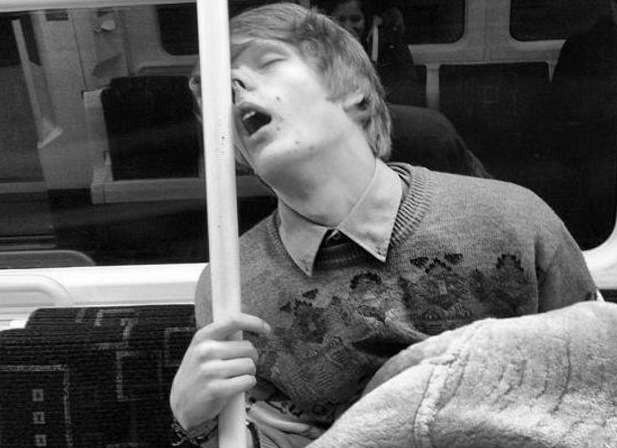
\includegraphics[width=\linewidth]{snore.jpg}
  \caption{If you wakeup from sleeping on a train moving at constant velocity, there is nothing about the physics in the train that tells you it's moving.  The constant velocity train is inertial and a legit frame of reference from which to do physics.}
  \label{fig:marginfig}
\end{marginfigure}
\newthought{Galilean invariance} or Galilean relativity states that the laws of motion are the same in all inertial frames. Galileo Galilei first described this principle in 1632 in his Dialogue Concerning the Two Chief World Systems using the example of a ship travelling at constant velocity, without rocking, on a smooth sea; any observer doing experiments below the deck would not be able to tell whether the ship was moving or stationary.  Newton's second law is invariant to change in the velocity of the frame.


\section{Newton's Third Law}
\newthought{The third law states} that all forces between two objects exist in equal magnitude and opposite direction: if object one exerts a force $\overrightarrow{F}_{ 1\rightarrow 2}$ on object two , then object two simultaneously exerts a force $\overrightarrow{F}_{ 2\rightarrow 1}$ on object one, and the two forces are equal in magnitude but opposite in direction.
$$\overrightarrow{F}_{ 1\rightarrow 2}=-\overrightarrow{F}_{2\rightarrow 1}$$

The third law means that all forces are interactions between different bodies,and thus that there is no such thing as a unidirectional force or a force that acts on only one body. This law is sometimes referred to as the action-reaction law, with $\overrightarrow{F}_{ 1\rightarrow 2}$ called the "action" and $\overrightarrow{F}_{ 2\rightarrow 1}$ the "reaction". The action and the reaction are simultaneous, and it does not matter which is called the action and which is called reaction; both forces are part of a single interaction, and neither force exists without the other.

\marginnote[-130pt]{\textit{To any action there is always an opposite and equal reaction; in other words, the actions of two bodies upon each other are always equal and always opposite in direction. }\\   \noindent\textbf{\textit{- Principia}}
}

\newthought{The contemporary mantra} for Newton's third law is uttered as follows.\\ \ \\ \textbf{Every action has an equal and opposite reaction.}

\begin{marginfigure}[-40pt]%
  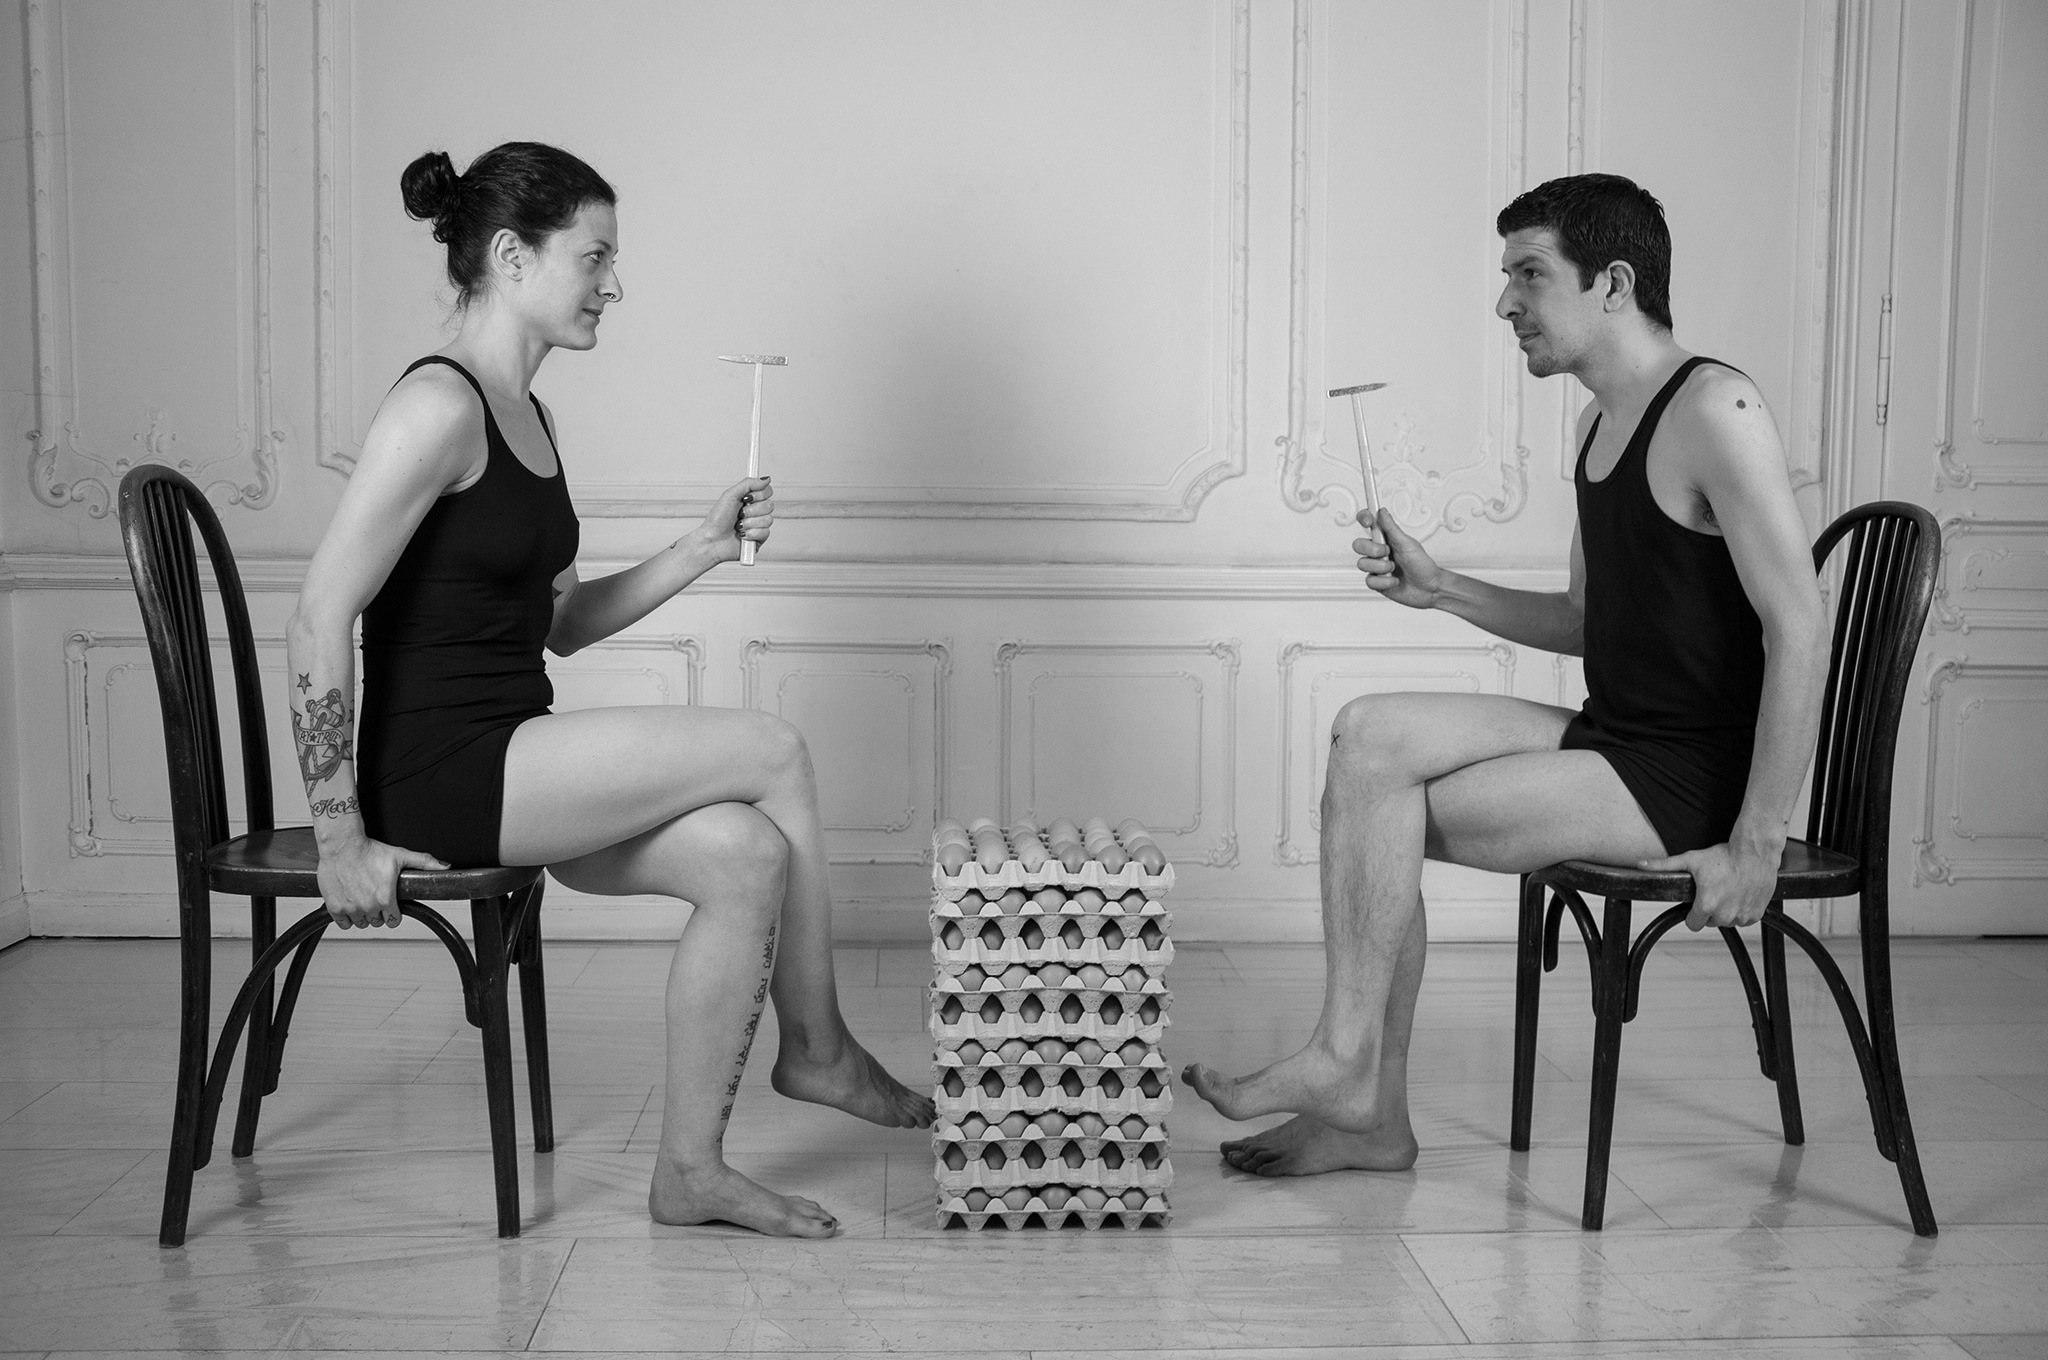
\includegraphics[width=\linewidth]{reaction.jpg}
  \caption{Action/Reaction was a 2014 performance art work by Rahman Hak-Hagir and Francesca Lolli.}
  \label{fig:marginfig}
\end{marginfigure}


\newpage

\section{Forces}
Forces are vector quantities as they had magnitudes and direction in space.  Summation of forces follows vector addition.   The unit of force is the Newton, or N.  This is one kilogram meter per square second.  

\marginnote[-40pt]{The English pound is a unit of force equivalent to $4.45$ Newtons.
$$1\ \text{lbs}=4.45\ \text{N}$$}

$$1\ \text{Newton}=\frac{\text{kg}\cdot\text{m}}{\text{s}^2}$$



\subsection{Statics}
\newthought{Statics is the branch of mechanics} that is concerned with the analysis of force loads on physical systems in static equilibrium, that is, in an inertial state where the relative positions of subsystems do not vary over time.  When in static equilibrium, the system is not being accelerated.  Therefore, by Newton's first law, the vector sum of the forces is zero.

\begin{marginfigure}[-50pt]%
  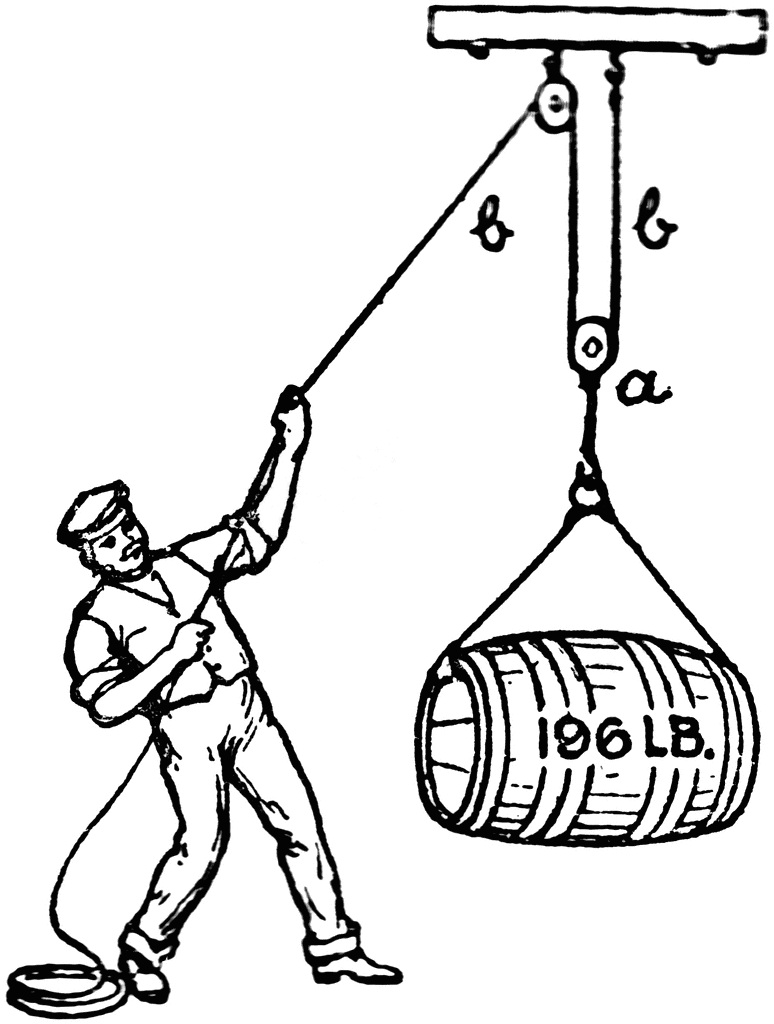
\includegraphics[width=\linewidth]{pulley.jpg}
  \caption{This could be a static or dynamic system, depending on the balance of forces.}
  \label{fig:marginfig}
\end{marginfigure}

\subsection{Dynamics} 
\newthought{Dynamics is the branch of mechanics} concerned with the study of forces and and their effect on motion.  In a dynamic situation the net force is non-zero and there is a resultant acceleration.  Newton's second law is invoked when analyzing a dynamic system. 



\section{Free Body Diagrams}
\newthought{A free body diagram is a graphical illustration} used to visualize and conceive of the applied forces on a body.  In the current treatment we represent particles with a dot and draw all forces incident on the particle as a vector diagram with all force vectors with their tail at the point.  

\marginnote[-70pt]{Once a coordinate system is established all forces can be decomposed in terms of components and summed across the component directions.  The resultant force determines the acceleration.  In some cases first knowing the acceleration gives an understanding of the constituent forces. }


\begin{fullwidth}
\vspace{0.5cm}
$$\overrightarrow{F}_{net}=\overrightarrow{F}_1+\overrightarrow{F}_2=\left(\begin{array}{c} \overrightarrow{F}_{2,x}  \\ \overrightarrow{F}_{1,y} +\overrightarrow{F}_{2,y}  \end{array}\right)=m\overrightarrow{a}\ \ \Longrightarrow \ \ \overrightarrow{a}=\frac{1}{m}\left(\begin{array}{c} \overrightarrow{F}_{2,x}  \\ \overrightarrow{F}_{1,y} +\overrightarrow{F}_{2,y}  \end{array}\right)$$
\vspace{0.5cm}
$$\begin{tikzpicture}[scale=1]
   	\draw[->,thick] (0,0) -- (0,-1) node [anchor=north ,scale=1] {$F_1 $}; 
     	\draw[->,thick] (0,0) -- ({2^0.5},{2^0.5}) node [anchor=south ,scale=1] {$F_2 $}; 
    	\fill[black] (0,0) circle (0.5mm);
    
     \begin{scope}[shift={(3,0.2)}, scale=0.75]
	  \draw[ thick,-stealth] (0,-0.1) -- (0,0.8) node [near start,anchor=east]{\scriptsize $y$};  
	  \draw[thick](-0.1,0) -- (0.1,0);
	   \draw[thick](0.2,-0.4) -- (0.2,-0.6);
	    \draw[ thick,-stealth] (0.1,-0.5) -- (1,-0.5) node [near start,anchor=north]{\scriptsize $x$};  
   \end{scope}

    
   \begin{scope}[shift={(5,0)}]
    	\draw[->,thick] (0,0) -- (0,-1) node [anchor=north ,scale=1] {$F_{1,y} $}; 
   	\draw[->,thick] (0,0) -- ({2^0.5},{0}) node [anchor=south ,scale=1] {$F_{2,x} $}; 
   	\draw[->,thick] (0,0) -- ({0},{2^0.5}) node [anchor=south ,scale=1] {$F_{2,y} $}; 
   	 \fill[black] (0,0) circle (0.5mm);
   \end{scope}
   
    \begin{scope}[shift={(8,0)}]   
   	  \draw[->,thick] (0,0) -- ({2^0.5 },{0}) node [anchor=south ,scale=1] {$F_{net,x} $}; 
   	   \draw[->,thick] (0,0) -- ({0},{2^0.5-1}) node [anchor=south ,scale=1] {$F_{net,y} $}; 
   	 \fill[black] (0,0) circle (0.5mm);
   \end{scope}
   
    \begin{scope}[shift={(11,0)}]
     	\draw[->,thick] (0,0) -- ({2^0.5 },{2^0.5-1}) node [anchor=south ,scale=1] {$F_{net} $};   
   	 \fill[black] (0,0) circle (0.5mm);
   \end{scope}
   
   \end{tikzpicture}
   $$
   \end{fullwidth}
\vspace{0.5cm}
\section{Weight}
\marginnote[30pt]{Modern work on gravitational theory began with the work of Galileo Galilei in the late 16th and early 17th centuries. In his famous (though possibly apocrypha) experiment dropping balls from the Tower of Pisa, and later with careful measurements of balls rolling down inclines, Galileo showed that gravity accelerates all objects at the same rate. This was a major departure from Aristotle's belief that heavier objects accelerate faster. Galileo postulated air resistance as the reason that lighter objects may fall more slowly in an atmosphere. Galileo's work set the stage for the formulation of Newton's theory of gravity.}
\newthought{Gravity is a natural phenomenon} by which all things with mass are brought towards (or 'gravitate' towards) one another including stars, planets, galaxies and even light and sub-atomic particles. Gravity is responsible for the complexity in the universe, by creating spheres of hydrogen, igniting them under pressure to form stars and grouping them into galaxies. Without gravity, the universe would be an uncomplicated one, existing without thermal energy and composed only of equally spaced particles. On Earth, gravity gives weight to physical objects and causes the tides. Gravity has an infinite range, and it cannot be absorbed, transformed, or shielded against.

\marginnote[60pt]{\textbf{Weight is the gravity force on a body.}}

Up until now mass has only been considered in its inertial properties.  Gravity is another feature of mass.  At the surface of the Earth, massive objects accelerate at a rate of $g=9.81\frac{\text{m}}{\text{s}^2}$.  Therefore by Newton's second law it follows that, at the surface of the Earth, the force due to gravity, otherwise known as the \textbf{weight}, is equal to $mg$.
\vspace{1cm}
\section{Constant Weight and Acceleration}
\marginnote[10pt]{The constant $g$ is the magnitude of acceleration due to gravity at the surface of the earth.  The direction of the acceleration is toward the center of the earth, namely down. }
$$g=9.81 \frac{\text{m}}{\text{s}^2}$$
\marginnote[20pt]{The force of gravity, or weight, is notated $\overrightarrow{F}_g$.}
$$F_g=mg$$
\vspace{0.5cm}
$$\overrightarrow{F}_{net}=\overrightarrow{F}_{g}=-\overbrace{m}^{\textit{Gravitational Mass}}g \hat{y}=\left(\begin{array}{c} 0 \\ -mg \end{array}\right)=m\overrightarrow{a}$$
\vspace{0.5cm}
$$\begin{tikzpicture}[scale=1]
 \begin{scope}[shift={(-5,0)}, scale=0.5]
\draw[very thick] (-1,-1) -- (-1,1) -- (1,1) -- (1,-1) -- cycle;  
\draw (0,0) node [anchor=center]{$m$};
 \end{scope}
 
  \begin{scope}[shift={(-2.5,-0.2)}, scale=0.75]
	 
	  \draw[ thick,-stealth] (0,-0.1) -- (0,0.8) node [near start,anchor=east]{\scriptsize $y$};  
	  \draw[thick](-0.1,0) -- (0.1,0);
	 
   	
   \end{scope}

     	\draw[->,thick] (0,0) -- (0,{-2^0.5}) node [anchor=north ,scale=1] {$F_g $}; 
    	\fill[black] (0,0) circle (0.5mm);   
   \end{tikzpicture}
   $$
   $$\overrightarrow{a}=\left(\begin{array}{c} 0  \\ -g \end{array}\right)$$
   
\section{Normal Force}
\marginnote[30pt]{The normal force ,$\overrightarrow{F}_n$ is the contact force between an object and a surface.  The direction of the normal force is directly out of the surface.  If there is no surface contact there is no normal force.}
\vspace{0.5cm}
$$\overrightarrow{F}_{net}=\overrightarrow{A}+\overrightarrow{F}_{n}=(F_n-A) \hat{y}=m\overrightarrow{a}$$
\vspace{0.5cm}
$$\begin{tikzpicture}[scale=1]
     	\draw[->,thick] (0,0) -- (0,{-1}) node [anchor=north ,scale=1] {$A$}; 
	\draw[->,thick] (0,0) -- (0,{2^0.5}) node [anchor=south ,scale=1] {$F_n $}; 
    	\fill[black] (0,0) circle (0.5mm);   
	
	  \begin{scope}[shift={(-5,0)}, scale=0.75]
	  \fill[color=gray!30, path fading=south] (-3,-1) -- (2.5,-1) -- (2.5,-2.5) -- (-3,-2.5) ;
	  \draw[very thick] (-3,-1) -- (2.5,-1) node [midway,anchor=north]{\scriptsize surface $\overrightarrow{a}_s$};  
	   \draw[ thick,-stealth] (-2.5,-1) -- (-2.5,-0.25) node [anchor=south]{$\hat{n}$};  
     	\draw[very thick] (-1,-1) -- (-1,1) -- (1,1) -- (1,-1) -- cycle;  
	 
	\draw (0,0) node [anchor=center]{$m$};
   	
   \end{scope}
   
   	  \begin{scope}[shift={(-1,0)}, scale=0.75]
	 
	  \draw[ thick,-stealth] (0,-0.1) -- (0,0.8) node [near start,anchor=east]{\scriptsize $y$};  
	  \draw[thick](-0.1,0) -- (0.1,0);
	 
   	
   \end{scope}
   \end{tikzpicture}
   $$
   \vspace{0.5cm}
   \marginnote[30pt]{As this free body diagram is drawn the normal force exceeds the applied force $\overrightarrow{A}$, therefore the object must be accelerating in the direction of the normal force.  This situation would arise in an upwardly accelerating elevator where the floor exerts a normal force on a passenger in excess of their weight.}
   
   $$\overrightarrow{a}=\frac{F_n-A}{m}\hat{y}$$
   $$F_n=A+ma_y$$
    $$\text{ surface contact requires\ \  }\ \overrightarrow{a}\cdot\hat{n}=\overrightarrow{a}_s\cdot\hat{n} \text{\ \   \   and     \ \ }(\overrightarrow{F}_n\cdot \hat{y})>0$$
     $$\text{for a non-accelerating surface }\ \overrightarrow{a}_s\cdot\hat{n}=0\ \ \ \Longrightarrow\ \ \ F_{net}=0\ \ \text{and}\ \ F_n=A$$
\vspace{0.5cm}

\section{Tension Force}
 \marginnote[30pt]{Tension describes the pulling force exerted by each end of a string, cable, chain, or similar one-dimensional continuous object, or by each end of a rod, truss member, or similar three dimensional object.}
\vspace{0.5cm}For simplicity this system is weightless.  
$$\overrightarrow{F}_{net}=\overrightarrow{T}=\left(\begin{array}{c} T_x \\ T_y \end{array}\right)=\left(\begin{array}{c} T\sin \theta \\ T\cos \theta \end{array}\right)=m\overrightarrow{a}$$
 \marginnote[60pt]{For simplicity this system is weightless.   The tension is drawn with horizontal and vertical components.  This will correspond to horizontal and vertical components of acceleration.}

\vspace{0.5cm}
$$\begin{tikzpicture}[scale=1]
     	
	\draw[->,thick] (0,0) -- (0.5,1.333) node [anchor=south ,scale=1] {$T$}; 
	\draw[dashed] (0,0) -- (0,1.3) node [midway, anchor=south west] {\tiny$\theta$};
    	\fill[black] (0,0) circle (0.5mm);   
	
	 \begin{scope}[shift={(3,0)}, scale=1]
	 \draw[->,thick] (0,0) -- (0,1.333) node [anchor=south ,scale=1] {$T_y$}; 
	 \draw[->,thick] (0,0) -- (0.5,0) node [anchor=west ,scale=1] {$T_x$}; 
	  \end{scope}
	
	
	  \begin{scope}[shift={(-5,-1)}, scale=0.5]
	  \draw[very thick] (0,1) -- (1.5,5); 
	   \draw[dashed] (1.5,5) -- (1.5,1.5) node [midway, anchor=north east] {\small$\theta$};; 
	  \fill[color=gray!30, path fading=north] (-3,5) -- (3,5) -- (3,7) -- (-3,7) ;
	  \draw[very thick] (-3,5) -- (3,5);  
	      	\draw[very thick] (-1,-1) -- (-1,1) -- (1,1) -- (1,-1) -- cycle;  
	 
	\draw (0,0) node [anchor=center]{$m$};
   	
   \end{scope}
   
   
   	  \begin{scope}[shift={(-2,0.2)}, scale=0.75]
	 
	  \draw[ thick,-stealth] (0,-0.1) -- (0,0.8) node [near start,anchor=east]{\scriptsize $y$};  
	  \draw[thick](-0.1,0) -- (0.1,0);
	   \draw[thick](0.2,-0.4) -- (0.2,-0.6);
	    \draw[ thick,-stealth] (0.1,-0.5) -- (1,-0.5) node [near start,anchor=north]{\scriptsize $x$};  
	 
   	
   
   
  
	 
   	
   \end{scope}
   \end{tikzpicture}
   $$
   
 
\newpage
\section{Friction Forces}
\marginnote[10pt]{Friction is the force resisting the relative motion of solid surfaces sliding against each other.  Friction is not itself a fundamental force. Dry friction arises from a combination of inter-surface adhesion, surface roughness, surface deformation, and surface contamination. The complexity of these interactions makes the calculation of friction from first principles impractical and necessitates the use of empirical methods.}
\subsection{Kinetic Friction}
\vspace{0.5cm}
\marginnote[10pt]{Kinetic friction is modeled as a force directly proportional to the normal force and in the opposite direction of sliding.  The constant of proportionality is termed $\mu_k$.}
$$\overrightarrow{F}_{f}=-\mu_kF_n \hat{v}$$
$$\overrightarrow{F}_{net}=\overrightarrow{A}+\overrightarrow{F}_{n}+\overrightarrow{F}_{f}=\left(\begin{array}{c} -F_f \\ F_n-A \end{array}\right)=m\overrightarrow{a}$$
\vspace{0.5cm}
$$\begin{tikzpicture}[scale=1]
     	\draw[->,thick] (0,0) -- (0,-1) node [anchor=north ,scale=1] {$A $}; 
	\draw[->,thick] (0,0) -- (0,1) node [anchor=south ,scale=1] {$F_n $}; 
	\draw[->,thick] (0,0) -- (-0.7,0) node [anchor=east ,scale=1] {$F_f $}; 
    	\fill[black] (0,0) circle (0.5mm);   
	
	  \begin{scope}[shift={(-5,0)}, scale=0.75]
	  \fill[color=gray!30, path fading=south] (-3,-1) -- (2.5,-1) -- (2.5,-2.5) -- (-3,-2.5) ;
	  \draw[very thick] (-3,-1) -- (2.5,-1) node [midway,anchor=north]{\scriptsize surface $\overrightarrow{a}_s=0$};  
	   \draw[ thick,-stealth] (-2.5,-1) -- (-2.5,-0.25) node [anchor=south]{$\hat{n}$};  
	     \draw[ thick,-stealth] (-0.5,1.5) -- (0.5,1.5) node [midway,anchor=south]{$\hat{v}$};  
     	\draw[very thick] (-1,-1) -- (-1,1) -- (1,1) -- (1,-1) -- cycle;  
	 
	\draw (0,0) node [anchor=center]{$m$};
   	
   \end{scope}
  
   
     \begin{scope}[shift={(2,0.2)}, scale=0.75]
	  \draw[ thick,-stealth] (0,-0.1) -- (0,0.8) node [near start,anchor=east]{\scriptsize $y$};  
	  \draw[thick](-0.1,0) -- (0.1,0);
	   \draw[thick](0.2,-0.4) -- (0.2,-0.6);
	    \draw[ thick,-stealth] (0.1,-0.5) -- (1,-0.5) node [near start,anchor=north]{\scriptsize $x$};  
	  \end{scope}
	  
	   \end{tikzpicture}$$
   $$\overrightarrow{a}=\frac{1}{m}\left(\begin{array}{c}- F_f  \\ F_n-A \end{array}\right)$$
   
   
     $$\text{for a non-accelerating surface }\ \overrightarrow{a}_s\cdot\hat{n}=0\ \ \ \Longrightarrow\ \ \ F_n=A$$
     $$F_f=\mu_kF_n=\mu_kA$$
     $$\overrightarrow{a}=\frac{1}{m}\left(\begin{array}{c} -\mu_kA  \\ 0 \end{array}\right)$$
     
     \subsection{Static Friction}
\vspace{0.5cm}
\marginnote[10pt]{Static friction is modeled as a force resisting sliding equal to the total applied shear force.  It keeps the object still until the static friction force is overcome.  The maximum magnitude of the friction force is modeled as directly proportional to the normal force.  The constant of proportionality is $\mu_s$.}

$${F_{f}}_{max}=\mu_sF_n$$
$$\overrightarrow{F}_{net}=\overrightarrow{A}+\overrightarrow{F}_{n}+\overrightarrow{F}_f=\left(\begin{array}{c} A_x-F_f \\ F_n-A_y \end{array}\right)=m\overrightarrow{a}=0$$
\vspace{0.5cm}
$$\begin{tikzpicture}[scale=1]
     	\draw[->,thick] (0,0) -- (0.7,-1) node [anchor=north ,scale=1] {$A $}; 
	\draw[->,thick] (0,0) -- (0,1) node [anchor=south ,scale=1] {$F_n $}; 
	\draw[->,thick] (0,0) -- (-0.7,0) node [anchor=east ,scale=1] {$F_f $}; 
    	\fill[black] (0,0) circle (0.5mm);   
	
	  \begin{scope}[shift={(-5,0)}, scale=0.75]
	  \fill[color=gray!30, path fading=south] (-3,-1) -- (2.5,-1) -- (2.5,-2.5) -- (-3,-2.5) ;
	  \draw[very thick] (-3,-1) -- (2.5,-1) node [midway,anchor=north]{\scriptsize surface $\overrightarrow{a}_s=0$};  
	   \draw[ thick,-stealth] (-2.5,-1) -- (-2.5,-0.25) node [anchor=south]{$\hat{n}$};  
	   
     	\draw[very thick] (-1,-1) -- (-1,1) -- (1,1) -- (1,-1) -- cycle;  
	 
	\draw (0,0) node [anchor=center]{$m$};
   	
   \end{scope}
     \begin{scope}[shift={(2,0.2)}, scale=0.75]
	  \draw[ thick,-stealth] (0,-0.1) -- (0,0.8) node [near start,anchor=east]{\scriptsize $y$};  
	  \draw[thick](-0.1,0) -- (0.1,0);
	   \draw[thick](0.2,-0.4) -- (0.2,-0.6);
	    \draw[ thick,-stealth] (0.1,-0.5) -- (1,-0.5) node [near start,anchor=north]{\scriptsize $x$};  
	  \end{scope}
   \end{tikzpicture}
   $$
   $$\text{if } A_x>{F_{f}}_{max}\ \ \ \Longrightarrow \ \ \ \text{kinetic}$$


\section{Sitting Under Gravity}
\marginnote[10pt]{This system is pretty boring.  Static.  Two forces, equal and opposite}
$$\begin{tikzpicture}[scale=1]
     	\draw[->,thick] (0,0) -- (0,{-1}) node [anchor=north ,scale=1] {$F_g$}; 
	\draw[->,thick] (0,0) -- (0,{1}) node [anchor=south ,scale=1] {$F_n $}; 
    	\fill[black] (0,0) circle (0.5mm);   
	
	  \begin{scope}[shift={(-5,0)}, scale=0.75]
	  \fill[color=gray!30, path fading=south] (-3,-1) -- (2.5,-1) -- (2.5,-2.5) -- (-3,-2.5) ;
	  \draw[very thick] (-3,-1) -- (2.5,-1) node [midway,anchor=north]{\scriptsize surface $\overrightarrow{a}_s=0$};  
	   \draw[ thick,-stealth] (-2.5,-1) -- (-2.5,-0.25) node [anchor=south]{$\hat{n}$};  
     	\draw[very thick] (-1,-1) -- (-1,1) -- (1,1) -- (1,-1) -- cycle;  
	 
	\draw (0,0) node [anchor=center]{$m$};
   	
   \end{scope}
   
   	  \begin{scope}[shift={(-1,0)}, scale=0.75]
	 
	  \draw[ thick,-stealth] (0,-0.1) -- (0,0.8) node [near start,anchor=east]{\scriptsize $y$};  
	  \draw[thick](-0.1,0) -- (0.1,0);
	 
   	
   \end{scope}
   \end{tikzpicture}
   $$
   
   $$\overrightarrow{F}_{net}=\overrightarrow{F}_{n}+\overrightarrow{F}_g=\left(\begin{array}{c} 0\\ F_n-mg \end{array}\right)=m\overrightarrow{a}=0$$
   
   $$F_n=mg$$
   
   
\section{Hanging Under Gravity and Horizontal Acceleration}
\marginnote[80pt]{This system is the jam!  It's a mix of statics and kinetics, a veritable physics explosion.  There is no acceleration in the vertical direction, only in the horizontal.}

$$\overrightarrow{F}_{net}=\overrightarrow{T}+\overrightarrow{F}_g=\left(\begin{array}{c} T_x \\ T_y-mg \end{array}\right)=\left(\begin{array}{c} T\sin \theta \\ T\cos \theta-mg \end{array}\right)=m\overrightarrow{a}=\left(\begin{array}{c} ma_x \\  0 \end{array}\right)$$
\vspace{0.5cm}
$$\begin{tikzpicture}[scale=1]
     	
	\draw[->,thick] (0,0) -- (0.5,1.333) node [anchor=south ,scale=1] {$T$}; 
	\draw[->,thick] (0,0) -- (0,-1.333) node [anchor=north ,scale=1] {$F_g$}; 
	\draw[dashed] (0,0) -- (0,1.3) node [midway, anchor=south west] {\tiny$\theta$};
    	\fill[black] (0,0) circle (0.5mm);   
	
	 \begin{scope}[shift={(3,0)}, scale=1]
	 \draw[->,thick] (0,0) -- (0,1.333) node [anchor=south ,scale=1] {$T_y$}; 
	 \draw[->,thick] (0,0) -- (0.5,0) node [anchor=west ,scale=1] {$T_x$}; 
	 \draw[->,thick] (0,0) -- (0,-1.333) node [anchor=north ,scale=1] {$F_g$}; 
	  \end{scope}
	
	
	  \begin{scope}[shift={(-5,-1)}, scale=0.5]
	  \draw[very thick] (0,1) -- (1.5,5); 
	   \draw[dashed] (1.5,5) -- (1.5,1.5) node [midway, anchor=north east] {\small$\theta$};; 
	  \fill[color=gray!30, path fading=north] (-3,5) -- (3,5) -- (3,7) -- (-3,7) ;
	  \draw[very thick] (-3,5) -- (3,5);  
	      	\draw[very thick] (-1,-1) -- (-1,1) -- (1,1) -- (1,-1) -- cycle;  
	 
	\draw (0,0) node [anchor=center]{$m$};
   	
   \end{scope}
   
   
   	  \begin{scope}[shift={(-2,0.2)}, scale=0.75] 
	  \draw[ thick,-stealth] (0,-0.1) -- (0,0.8) node [near start,anchor=east]{\scriptsize $y$};  
	  \draw[thick](-0.1,0) -- (0.1,0);
	   \draw[thick](0.2,-0.4) -- (0.2,-0.6);
	    \draw[ thick,-stealth] (0.1,-0.5) -- (1,-0.5) node [near start,anchor=north]{\scriptsize $x$};  
	  \end{scope}
   \end{tikzpicture}
   $$
   
   \marginnote[10pt]{Given the angle we can determine the acceleration in the horizontal direction.  Fuzzy dice hanging from the rearview window are effectively an accelerometer.}
   
 $$ T\cos \theta=mg$$
 $$ T\sin \theta=ma_x$$
 \vspace{1cm}
 $$T=m\sqrt{g^2+a_x^2}$$
 $$\theta=\tan^{-1}\left(\frac{a_x}{g}\right)$$
 
 \newpage
 
 \section{Inclined Plane with Friction}
 
 $$\overrightarrow{F}_{net}=\overrightarrow{F}_g+\overrightarrow{F}_n+\overrightarrow{F}_f=\left(\begin{array}{c} F_f-F_{g,x} \\ F_n-F_{g,y} \end{array}\right)=\left(\begin{array}{c} F_f-mg\sin \theta \\ F_n-mg\cos \theta \end{array}\right)=m\overrightarrow{a}=\left(\begin{array}{c} ma_x \\  0 \end{array}\right)$$

\marginnote[70pt]{This system is best modeled by applying a rotated coordinate system so that $x$ is in the direction of motion and $y$ is normal to the surface of the inclined plane.}
 
 
 $$\begin{tikzpicture}[scale=1]
     	\draw[->,thick] (0,0) -- (0,{-1}) node [anchor=north ,scale=1] {$F_g$}; 
	\begin{scope}[rotate=30]
	\draw[->,thick] (0,0) -- (0,{cos(30)}) node [anchor=south ,scale=1] {$F_n $}; 
	\draw[->,thick] (0,0) -- (1,0) node [anchor=west ,scale=1] {$F_f $}; 

	\end{scope}
    	\fill[black] (0,0) circle (0.5mm);   
	
	  \begin{scope}[shift={(3,0)}]
	  \begin{scope}[rotate=30]
	  \draw[->,thick] (0,0) -- (0,{-cos(30)}) node [anchor=north ,scale=1] {$F_{g,y}$}; 
	   \draw[->,thick] (0,0) -- (-0.5,0) node [anchor=north ,scale=1] {$F_{g,x}$}; 
	   \draw[->,thick] (0,0) -- (1,0) node [anchor=west ,scale=1] {$F_f $}; 
	
	\draw[->,thick] (0,0) -- (0,{cos(30)}) node [anchor=south ,scale=1] {$F_n $}; 
	\end{scope}
    	\fill[black] (0,0) circle (0.5mm); 
	\end{scope}
	
	  \begin{scope}[shift={(-5,0)}, scale=0.75, rotate=30]
	  \fill[color=gray!30, path fading=south] (-3,-1) -- (2.5,-1) -- (2.5,-2.5) -- (-3,-2.5) ;
	  \draw[very thick] (-3,-1) -- (2.5,-1);  
	   \draw[ thick,-stealth] (-2.5,-1) -- (-2.5,-0.25) node [anchor=south]{$\hat{n}$};  
     	\draw[very thick] (-1,-1) -- (-1,1) -- (1,1) -- (1,-1) -- cycle;  
	 
	\draw (0,0) node [anchor=center]{$m$};
	
	  \draw[ thick,-stealth] (0.5,1.5) -- (-0.5,1.5)   node [midway,anchor=south]{$\hat{v}$};  
   	
	  \begin{scope}[shift={(-3,-1)}, scale=0.75,rotate=-30]
	  \draw[dashed] (0,0) -- (3,0) node [midway, anchor=south] {\scriptsize$\theta$};
	  \end{scope}

	
   \end{scope}
   
   	  \begin{scope}[shift={(-2,0.2)}, scale=0.75,rotate=30] 
	  \draw[ thick,-stealth] (0,-0.1) -- (0,0.8) node [near start,anchor=east]{\scriptsize $y$};  
	  \draw[thick](-0.1,0) -- (0.1,0);
	   \draw[thick](0.2,-0.4) -- (0.2,-0.6);
	    \draw[ thick,-stealth] (0.1,-0.5) -- (1,-0.5) node [near start,anchor=north]{\scriptsize $x$};  
	  \end{scope}   	
		
	 \end{tikzpicture}
   $$
$$F_n=mg\cos \theta$$
$$F_f=\mu mg\cos \theta$$
$$a_x=\mu g\cos \theta-g\sin \theta$$

\section{Atwood's Machine}
\marginnote[70pt]{The Atwood machine (or Atwood's machine) was invented in 1784 by the English mathematician George Atwood as a laboratory experiment to verify the mechanical laws of motion with constant acceleration. Atwood's machine is a common classroom demonstration used to illustrate principles of classical mechanics.  The ideal Atwood Machine consists of two objects of mass $m_1$ and $m_2$, connected by an inextensible massless string over an ideal massless pulley.}


$$\begin{tikzpicture}[scale=1]
     	
	
	
\begin{scope}[shift={(0,0)}, scale=1]
	\fill[color=gray!20] (0,0) circle (1cm);
	\draw[very thick] (0,0) circle (1cm);
	\draw[thick] (1,0) -- (1,-2.5); 
	\draw[thick] (-1,0) -- (-1,-2.5); 
	\draw[very thick] (-1.5,-2.5) -- (-0.5,-2.5) -- (-0.5,-3.5) -- (-1.5,-3.5) -- cycle;
	\draw (-1,-3) node [anchor=center] {$m_1$};
	\draw[very thick] (1.5,-2.5) -- (0.5,-2.5) -- (0.5,-4) -- (1.5,-4) -- cycle;
	\draw (1,-3) node [anchor=center] {$m_2$};	
\end{scope}

   	  \begin{scope}[shift={(-2,-1)}, scale=0.75,rotate=0] 
	  \draw[ thick,-stealth] (0,-0.1) -- (0,0.8) node [near start,anchor=east]{\scriptsize $y$};  
	  \draw[thick](-0.1,0) -- (0.1,0);
	  \end{scope}
	  
	    \begin{scope}[shift={(2,-1)}, scale=0.75,rotate=180] 
	  \draw[ thick,-stealth] (0,-0.1) -- (0,0.8) node [near start,anchor=east]{\scriptsize $y$};  
	  \draw[thick](-0.1,0) -- (0.1,0);
	  \end{scope}
	  
	  \begin{scope}[shift={(-5,-2)}, scale=1,rotate=0] 
	  \draw[->,thick] (0,0) -- (0,1.3) node [anchor=south ,scale=1] {$T$}; 
	\draw[->,thick] (0,0) -- (0,-1) node [anchor=north ,scale=1] {$m_1g $}; 
    	\fill[black] (0,0) circle (0.5mm);   
	  \end{scope}
	  
	   \begin{scope}[shift={(5,-2)}, scale=1,rotate=0] 
	  \draw[->,thick] (0,0) -- (0,1.3) node [anchor=south ,scale=1] {$T$}; 
	\draw[->,thick] (0,0) -- (0,-1.5) node [anchor=north ,scale=1] {$m_2g $}; 
    	\fill[black] (0,0) circle (0.5mm);   
	  \end{scope}
	  
	 
    
   \end{tikzpicture}
   $$
   $$\text{1:}\ \ \ \overrightarrow{F}_{1,net}=\overrightarrow{F}_{1,g}+\overrightarrow{T}_1=(\ \ T-m_1g)\hat{y}=m_1\overrightarrow{a}$$
    $$\text{2:}\ \ \ \overrightarrow{F}_{2,net}=\overrightarrow{F}_{2,g}+\overrightarrow{T}_2=(-T+m_2g)\hat{y}=m_2\overrightarrow{a}$$

$$T-m_1g=m_1a$$
$$-T+m_2g=m_2a$$

$$ a=\frac{g(m_2-m_1)}{m_1+m_2} \ \ \ \text{and} \ \ \  T=\frac{(m_1-m_2)a+(m_1+m_2)g}{2}=\frac{2gm_1m_2}{m_1+m_2}$$

\section{Circular Motion}

\marginnote[10pt]{Circular motion is best analyzed determining the components of force in the tangential and radial direction.  The net radial force functions as the centripetal force.  The tangential components of the forces change the speed of the mass. }




$$\begin{tikzpicture}[scale=1]
     	
	
	
\draw [color=gray!80] (0,0)--(3,0)
   node [midway,anchor=south,inner sep=1pt, outer sep=1pt]{$R$};


 \begin{scope}[shift={(0,0)}, scale=1,rotate=120] 
 \draw[color=gray,dashed] (0,0) circle (3cm);
  \begin{scope}[shift={(0,-4)}, scale=0.75, rotate=-90] 
	  \draw[ thick,-stealth] (0,-0.1) -- (0,0.8) node [near start,anchor=east]{\scriptsize $\theta$};  
	  \draw[thick](-0.1,0) -- (0.1,0);
	   \draw[thick](0.2,-0.4) -- (0.2,-0.6);
	    \draw[ thick,-stealth] (0.1,-0.5) -- (1,-0.5) node [near start,anchor=north]{\scriptsize $r$};  
	  \end{scope}
 \fill[black] (0,0) circle (1mm);  
 \draw [very thick] (0,0) -- (0,-3);
 \fill[color=white] (0.5,-2.5) -- (-0.5,-2.5) -- (-0.5,-3.5) -- (0.5,-3.5) -- cycle;
  \draw[very thick] (0.5,-2.5) -- (-0.5,-2.5) -- (-0.5,-3.5) -- (0.5,-3.5) -- cycle;
  \draw (0,-3) node {$m$};
 \end{scope}
		  
	   \begin{scope}[shift={(9,0)}, scale=1,rotate=120] 
	  \draw[->,thick] (0,0) -- (0,1.3) node [anchor=east ,scale=1] {$F_{c}$}; 
	   \draw[->,thick] (0,0) -- (-0.7,0) node [anchor=north ,scale=1] {$F_{t}$}; 
    	\fill[black] (0,0) circle (0.5mm);   
	  \end{scope}
	  
	    \begin{scope}[shift={(6,0)}, scale=1,rotate=120] 
	
	   \draw[->,thick] (0,0) -- (-0.7,1.3) node [anchor=north ,scale=1] {$F_{net}$}; 
    	\fill[black] (0,0) circle (0.5mm);   
	  \end{scope}
	  
	  
    
   \end{tikzpicture}$$
   $$\overrightarrow{F}_{net}=m\overrightarrow{a}=mr\ddot{\theta}\hat{\theta}-m r\dot{\theta}^2\hat{r}$$
   $$F_t=mr\ddot{\theta}=mr\alpha=ma_t$$
   $$F_c=mr\omega^2=m\frac{v^2}{r}=ma_c$$
\section{Non-Inertial Frames}
\marginnote[20pt]{In a non-inertial frame a fictional force is observed in the opposite direction of the acceleration of the frame.  For example, a frame accelerated centripetally will exhibit a centrifugal pseudo-force.  The Coriolis effect is another example of pseudo-forces in action. }
$$\begin{tikzpicture}[scale=1]
     	
	 \draw[color=gray,dashed] (-2,-2) -- (2,-2) -- (2,2) -- (-2,2) -- cycle;
	  \draw [thick,->] (2,2) -- (3,1.5) node [anchor=west]{$\overrightarrow{a}_{frame}$};
	  
	

 \draw[->,thick] (0,0) -- (-1,0.5) node [anchor=south ,scale=1] {$\overrightarrow{F}_{pseudo}$}; 
    	\fill[black] (0,0) circle (0.5mm);   


	  \draw (6,0) node {$\overrightarrow{F}_{pseudo}=-m\overrightarrow{a}_{frame}$};
	  
    
   \end{tikzpicture}$$
   



\section{Accelerometers}
$$\begin{tikzpicture}[scale=1]
     	
	 \draw[color=gray,dashed] (-2,-2) -- (2,-2) -- (2,2) -- (-2,2) -- cycle;
	  \draw [thick,->] (2,2) -- (3,1.5) node [anchor=west]{$\overrightarrow{a}_{frame}$};
	  
	
\draw[->,thick] (0,0) -- (0,-1) node [anchor=north,scale=1] {$\overrightarrow{F}_{g}$}; 
 \draw[->,thick] (0,0) -- (-1,0.5) node [anchor=south ,scale=1] {$\overrightarrow{F}_{pseudo}$}; 
    	\fill[black] (0,0) circle (0.5mm);   


\draw (6,0) node {$\overrightarrow{F}_{accel}=\overrightarrow{F}_{pseudo}+\overrightarrow{F}_{g}$};
	  
    
   \end{tikzpicture}$$
   



\section{Universal Gravitational Force}
\marginnote[0pt]{Newton's law of universal gravitation states that any two bodies in the universe attract each other with a force that is directly proportional to the product of their masses and inversely proportional to the square of the distance between them.}

$$F_g=\frac{Gm_1m_2}{r^2} \hspace{1cm} G=6.674\times10^{-11} \frac{\text{N}\cdot\text{m}^2}{\text{kg}^2}$$
$${\overrightarrow{F}_{g}}_{1\rightarrow 2}=-\frac{Gm_1m_2}{r^2}\hat{r}=-{\overrightarrow{F}_{g}}_{2\rightarrow 1}$$


$$\begin{tikzpicture}[scale=1]
     	
	\fill[black] (-7,0) circle (0.5mm);   
	\draw[->,thick] (-7,0) -- (-6,0) node [anchor=west ,scale=1] {$F_g$}; 
	\fill[black] (7,0) circle (0.5mm);   
	\draw[->,thick] (7,0) -- (6,0) node [anchor=east ,scale=1] {$F_g$}; 
	 \draw[very thick] (-4,0) circle (0.5cm) node {$m_1$};
	  \draw[very thick] (4,0) circle (0.5cm) node {$m_2$};
	    \draw[thick, color=gray,->] (-4,-0.75) --   (4,-0.75) node [midway, anchor=south] {$r$};
	     
	     
	       \begin{scope}[shift={(-3,0)}, scale=0.75] 
	 
	   \draw[thick](0.2,0.1) -- (0.2,-0.1);
	    \draw[ thick,-stealth] (0.1,0) -- (1,0) node [near start,anchor=north]{\scriptsize $r$};  
	  \end{scope}
   
	     
   \end{tikzpicture}$$


\section{Spring Force}
\marginnote[0pt]{Hooke's law states that the force needed to extend or compress a spring by some distance is directly proportional to that distance.  The proportionality constant, $k$, is known as the spring constant.  The law is named after 17th century British physicist Robert Hooke. Hooke's equation in fact holds (to some extent) in many other situations where an elastic body is deformed, such as wind blowing on a tall building, a musician plucking a string of a guitar, or the filling of a party balloon. An elastic body or material for which this equation can be assumed is said to be linear-elastic or Hookean.}


$$\overrightarrow{F}_k=-k\overrightarrow{x}$$
$$\overrightarrow{F}_{net}=\overrightarrow{F}_k= -kx\hat{x}=m\overrightarrow{a}$$

\tikzstyle{spring}=[thick,decorate,decoration={zigzag,pre length=0.1cm,post
  length=0.1cm,segment length=6}]
  
  $$\begin{tikzpicture}[scale=1]
     	
	\draw[->,thick] (0,0) -- (0,1) node [anchor=south ,scale=1] {$F_k$}; 
	
	
    	\fill[black] (0,0) circle (0.5mm);   
	
	
	
	
	  \begin{scope}[shift={(-5,-1)}, scale=0.5]
	 \draw[dashed, color=gray] (-3,3) -- (3,3) node [near start, anchor =south east] {\tiny equilibrium};
	 	\draw[spring] (0,1) -- (0,5);
		 \draw[->,thick, color=gray] (2,3) -- (2,0) node [midway, anchor =west] {\small$\overrightarrow{x}$};
	  \fill[color=gray!30, path fading=north] (-3,5) -- (3,5) -- (3,7) -- (-3,7) ;
	  \draw[very thick] (-3,5) -- (3,5);  
	      	\draw[very thick] (-1,-1) -- (-1,1) -- (1,1) -- (1,-1) -- cycle;  
	 
	\draw (0,0) node [anchor=center]{$m$};
   	
   \end{scope}
   
   
   	  \begin{scope}[shift={(-2,0.2)}, scale=0.75, rotate=180] 
	  \draw[ thick,-stealth] (0,-0.1) -- (0,0.8) node [near start,anchor=east]{\scriptsize $x$};  
	  \draw[thick](-0.1,0) -- (0.1,0);  
	  \end{scope}
   \end{tikzpicture}
   $$
  
\section{Time Dependent Forces}
$$\overrightarrow{F}=\overrightarrow{F}(t)$$
\begin{itemize}
  \item Propulsion, Wind, Tide, etc
\end{itemize}

\marginnote{
  
\includegraphics[width=\linewidth]{special-forces.jpg}}


\section{Space Dependent Forces}
$$\overrightarrow{F}=\overrightarrow{F}(\overrightarrow{\scriptr})$$
\begin{itemize}
  \item Spring, Universal Gravity, Electromagnetic Forces, etc
\end{itemize}
\section{Velocity Dependent Forces}
$$\overrightarrow{F}=\overrightarrow{F}(\overrightarrow{v})$$
\begin{itemize}
  \item Drag, Magnetic Force, etc
\end{itemize}


\chapter{Work, Energy and Power}
\begin{marginfigure}%
  
\includegraphics[width=\linewidth]{gotowork.jpg}
  \caption{Kool Moe Dee recorded the 1989 single \textit{I Go to Work}.}
  \label{fig:marginfig}
\end{marginfigure}
\textit{Work alone is noble.}  \\
\noindent\textbf{-   Thomas Carlyle}

\vspace{1cm}

\section{Work}

\marginnote[20pt]{Work is the accumulated effect of a force on a mass moving through space.}

\newthought{A force is said to do work if}, when acting on a body, there is a displacement of the point of application in the direction of the force.
 For example, when a ball is held above the ground and then dropped, the work done on the ball as it falls is equal to the weight of the ball (a force) multiplied by the distance to the ground (a displacement).  The term work was introduced in 1826 by the French mathematician Gaspard-Gustave Coriolis as "weight lifted through a height", which is based on the use of early steam engines to lift buckets of water out of flooded ore mines.

\subsection{1-D}
Mathematically, the accumulation of work is expressed as a sum terms of force times displacement.  
$$W=\sum_i F(x_i) \Delta{x}_i$$
Graphically, this corresponds to the area under the curve of $F(x)$.
$$W=\text{Area}(F(x))$$

\begin{marginfigure}[-150pt]%
  \begin{tikzpicture}
    [line cap=round,line join=round,x=2cm,y=2cm, scale=1.5, decoration={brace,amplitude=2pt}]
%main layer
%creating the ticks and xy-axis nodes
%some function
\fill[fill=red!20] (0.25,0) -- plot [domain=0.25:.75] (\x,{-\x^2/2+\x+0.25}) -- plot [domain=0.75: 0.25] (\x,0) -- cycle;

 \draw[smooth,samples=200,domain=0.25:0.75]
                                 plot(\x,{-\x^2/2+\x+0.25});
 

    \fill[black] (0.25,0) circle (0.3mm) node [anchor=north ,scale=1] {$ a$};
     \fill[black] (0.75,0) circle (0.3mm) node [anchor=north ,scale=1] {$b$};
      %  \fill[black] (0,0.25) circle (0.3mm) node [anchor=south east,scale=1] {\scriptsize$ v(0)$};

  \draw[-latex,color=black,thin] (-0.2,0) -- (1.4,0) node [anchor=north ,scale=1] {$x$};
   \draw[-latex,color=black,thin] (0,-0.2) -- (0,1.4)node [anchor=east ,scale=1] {$F$};
    \draw (0.6,0.8) node [anchor=south west ,scale=1] {$F(x)$};
        \draw (0.5,0.25) node [anchor=center ,scale=1] {$W$};
        
 \end{tikzpicture}
  \caption{Work is the area under the curve in a force versus position graph.}
  \label{fig:marginfig}
\end{marginfigure}


\newpage

\subsubsection{Case: Constant Force}
\newthought{In the case of constant force}, the work is graphically represented by a rectangular area.  Consider the constant force of gravity on a mass.  The work done by gravity is the product of the weight and the displacement.  With downward motion gravity does positive work.  In upward motion, gravity does negative work.
\begin{marginfigure}[-50pt]%
  \begin{tikzpicture}
    [line cap=round,line join=round,x=2cm,y=2cm, scale=1.5, decoration={brace,amplitude=2pt}]
%main layer
%creating the ticks and xy-axis nodes
%some function
\fill[fill=red!20] (0.25,0) --(0.25, 0.62) -- (0.75, 0.62) -- (0.75,0.0) -- cycle;

 \draw (0.25, 0.62) -- (0.75, 0.62) ;
 

    \fill[black] (0.25,0) circle (0.3mm) node [anchor=north ,scale=1] {$ a$};
     \fill[black] (0.75,0) circle (0.3mm) node [anchor=north ,scale=1] {$b$};
      %  \fill[black] (0,0.25) circle (0.3mm) node [anchor=south east,scale=1] {\scriptsize$ v(0)$};

  \draw[-latex,color=black,thin] (-0.2,0) -- (1.4,0) node [anchor=north ,scale=1] {$x$};
   \draw[-latex,color=black,thin] (0,-0.2) -- (0,1.4)node [anchor=east ,scale=1] {$F$};
    \draw (0.6,0.8) node [anchor=south west ,scale=1] {$F(x)=\text{constant}$};
        \draw (0.5,0.25) node [anchor=center ,scale=1] {$W$};
        
 \end{tikzpicture}
  \caption{For a constant force, work is simply $F\cdot d$.}
  \label{fig:marginfig}
\end{marginfigure}

$$W=\text{Area}(F(x))$$
$$W=F(b-a)=F\Delta x$$

\vspace{1cm}

\subsubsection{Case: Linear Force}
\newthought{In the case of a force that is linearly proportional} to position, the work is graphically represented by the familiar region shown in Figure \ref{fig:linearwork}.  This area bay be represented mathematically as the difference between two triangular regions.

\begin{marginfigure}[0pt]%
\begin{tikzpicture}
    [line cap=round,line join=round,x=2cm,y=2cm, scale=1.5, decoration={brace,amplitude=2pt}]
%main layer
%creating the ticks and xy-axis nodes
%some function
\fill[fill=red!20] (0.25,0) --(0.25, 0.25) -- (0.75, 0.75) -- (0.75,0.0) -- cycle;

 \draw (0.25, 0.25) -- (0.75, 0.75) ;
 

    \fill[black] (0.25,0) circle (0.3mm) node [anchor=north ,scale=1] {$ a$};
     \fill[black] (0.75,0) circle (0.3mm) node [anchor=north ,scale=1] {$b$};
      %  \fill[black] (0,0.25) circle (0.3mm) node [anchor=south east,scale=1] {\scriptsize$ v(0)$};

  \draw[-latex,color=black,thin] (-0.2,0) -- (1.4,0) node [anchor=north ,scale=1] {$x$};
   \draw[-latex,color=black,thin] (0,-0.2) -- (0,1.4)node [anchor=east ,scale=1] {$F$};
    \draw (0.6,0.8) node [anchor=south west ,scale=1] {$F(x)=kx$};
        \draw (0.5,0.25) node [anchor=center ,scale=1] {$W$};
        
 \end{tikzpicture}
  \caption{For a linear force, work is simply $\braket{F}\cdot d$.}
  \label{fig:linearwork}
\end{marginfigure}

$$W=\text{Area}(F(x))$$
$$W=\frac{kb^2}{2}-\frac{ka^2}{2}$$
$$W=\frac{k}{2}\left( b^2-a^2\right)=\frac{k}{2}\ \Delta( x^2)$$


 \subsection{2-D \& 3-D}

 \marginnote[0pt]{In higher dimensions, work is calculated as the dot product of the force and displacement vector.  For an arbitrary path sum the work over each section of the path.
 $$W=\sum_i \overrightarrow{F} \cdot \Delta{\overrightarrow{r}}_i$$}

The dot product is used to calculate work.  One interpretation is the product of displacement and force in the direction of displacement. 

\vspace{1cm}

 $$W=\overrightarrow{F}\cdot \Delta \overrightarrow{r}=F_{||} \  \Delta \overrightarrow{r}=F\cos\theta \  \Delta\overrightarrow{r}$$

\vspace{1cm}

$$
\begin{tikzpicture}[scale=1]
\draw [thick,->] (0,0) -- (2.1,2.3) node[anchor=south,color=black]{$\overrightarrow{F}$};
\draw [thick,->] (0,0) -- (1.8,0) node[midway, anchor=south east,color=black]{\small $\theta$} node[anchor=west,color=black]{\footnotesize$\Delta\overrightarrow{r}$};
\end{tikzpicture}
$$

\begin{marginfigure}[-80pt]%
\begin{tikzpicture}[scale=1.5]
\draw (2,0) node [anchor=north,scale=1] {$x $};
\draw (0,2) node [anchor=east,scale=1] {$y $};
\draw[->] (0,0) -- (2,0); 
\draw[->] (0,0) -- (0,2);
\fill[black] (0.45cm,1.05cm) circle (0.3mm);
\fill[black] (1.05cm,0.45cm) circle (0.3mm);
\draw (1,1) node [anchor=south west,scale=1] {$\{\Delta\overrightarrow{r}\}$};
\draw (0.5,1) node [anchor=south,scale=1] {$\ \ a$};
\draw (1,0.5) node [anchor=west,scale=1] {$\ b$};
\draw (0.5cm,1cm) [->,line width=0.2ex]  .. controls (0.6,0.6) and (0.8,0.8) ..   (1cm,0.5cm); 
\end{tikzpicture}
  \caption{Accumulation of work over a path.}
  \label{fig:linearwork}
\end{marginfigure}



\subsection{Unit}
\begin{marginfigure}%
  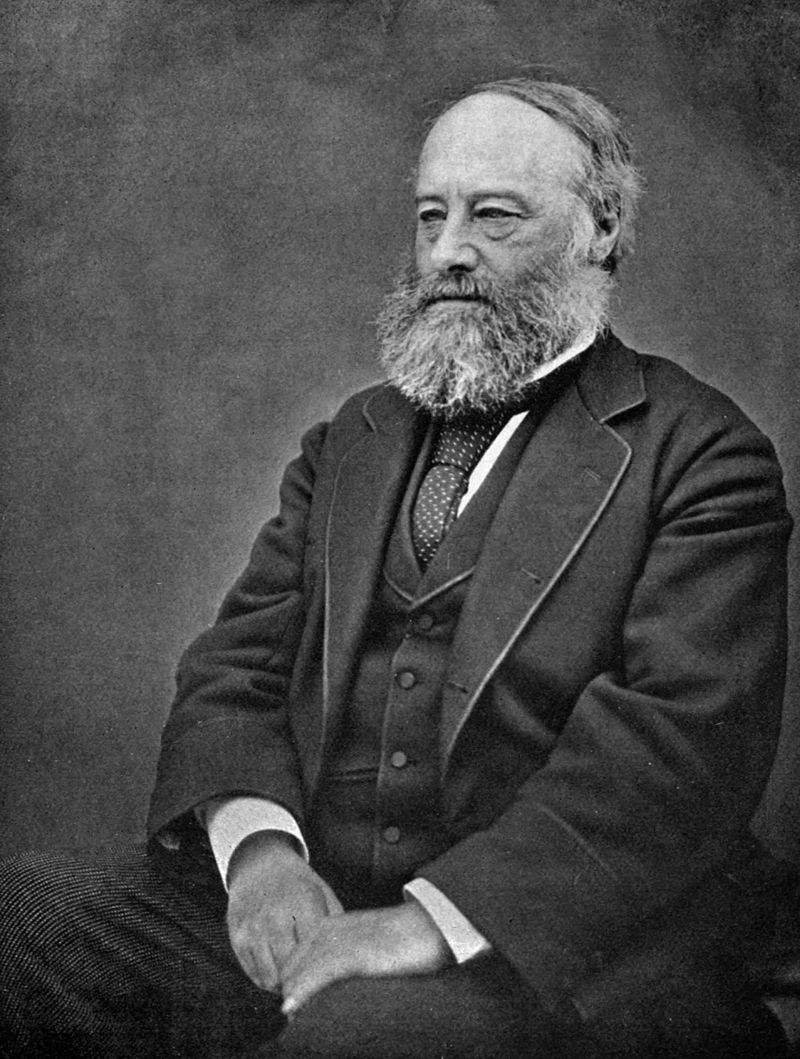
\includegraphics[width=\linewidth]{joule.jpg}
  \caption{James Joule rocked a three-piece suit.}
  \label{fig:marginfig}
\end{marginfigure}
\newthought{The Joule}, symbol J, is a derived unit of work and energy in the International System of Units.  It is equal to the work done to an object when a force of one newton acts on that object in the direction of its motion through a distance of one meter.  It is named after the English physicist James Prescott Joule (1818-1889).
$$\text{Joule}=\text{Newton}\cdot \text{meter}$$

\vspace{1cm}

\section{Power}
Power is the rate of doing work. It is equivalent to an amount of energy consumed per unit time. 
\begin{marginfigure}[0pt]%
  \begin{tikzpicture}
    [line cap=round,line join=round,x=2cm,y=2cm, scale=1.5, decoration={brace,amplitude=2pt}]
%main layer
%creating the ticks and xy-axis nodes
%some function
\fill[fill=red!20] (0.25,0) -- plot [domain=0.25:.75] (\x,{-\x^2/2+\x+0.25}) -- plot [domain=0.75: 0.25] (\x,0) -- cycle;

 \draw[smooth,samples=200,domain=0.25:0.75]
                                 plot(\x,{-\x^2/2+\x+0.25});
 

    \fill[black] (0.25,0) circle (0.3mm) node [anchor=north ,scale=1] {$ a$};
     \fill[black] (0.75,0) circle (0.3mm) node [anchor=north ,scale=1] {$b$};
      %  \fill[black] (0,0.25) circle (0.3mm) node [anchor=south east,scale=1] {\scriptsize$ v(0)$};

  \draw[-latex,color=black,thin] (-0.2,0) -- (1.4,0) node [anchor=north ,scale=1] {$t$};
   \draw[-latex,color=black,thin] (0,-0.2) -- (0,1.4)node [anchor=east ,scale=1] {$P$};
    \draw (0.6,0.8) node [anchor=south west ,scale=1] {$P(t)$};
        \draw (0.5,0.25) node [anchor=center ,scale=1] {$W$};
        
 \end{tikzpicture}
  \caption{Work is the area under the curve in a force versus position graph.}
  \label{fig:marginfig}
\end{marginfigure}

$$P=\frac{W}{\Delta t}$$
$$W=\text{Area}(P(t))$$
$$P=\frac{W}{\Delta t}=\frac{\overrightarrow{F}\cdot \Delta \overrightarrow{r}}{\Delta t}$$
$$P=\overrightarrow{F}\cdot  \overrightarrow{v}$$

\subsection{Unit}
\marginnote[5pt]{James Watt (1736-1819) was a Scottish inventor and mechanical engineer whose Watt steam engine was fundamental to the Industrial Revolution.}
In the SI system, the unit of power is the joule per second (J/s), known as the watt in honor of James Watt, the eighteenth-century developer of the steam engine.
$$\text{Watt}=\frac{\text{Joule}}{\text{second}}$$



\section{Kinetic Energy}
\begin{marginfigure}[20pt]%
\begin{tikzpicture}
    [line cap=round,line join=round,x=2cm,y=2cm, scale=1.5, decoration={brace,amplitude=2pt}]
%main layer
%creating the ticks and xy-axis nodes
%some function
\fill[fill=red!20] (0.25,0) --(0.25, 0.25) -- (0.75, 0.75) -- (0.75,0.0) -- cycle;

 \draw (0.25, 0.25) -- (0.75, 0.75) ;
 

    \fill[black] (0.25,0) circle (0.3mm) node [anchor=north ,scale=1] {$ v_1$};
     \fill[black] (0.75,0) circle (0.3mm) node [anchor=north ,scale=1] {$v_2$};
      %  \fill[black] (0,0.25) circle (0.3mm) node [anchor=south east,scale=1] {\scriptsize$ v(0)$};

  \draw[-latex,color=black,thin] (-0.2,0) -- (1.4,0) node [anchor=north ,scale=1] {$v$};
   \draw[-latex,color=black,thin] (0,-0.2) -- (0,1.4)node [anchor=east ,scale=1] {$p$};
    \draw (0.6,0.8) node [anchor=south west ,scale=1] {$p(v)=mv$};
        \draw (0.5,0.25) node [anchor=center ,scale=1] {$\Delta KE$};
        
 \end{tikzpicture}
  \caption{Kinetic energy expressed as the area under p(v).}
  \label{fig:marginfig}
\end{marginfigure}

\newthought{The kinetic energy} of an object is the energy that it possesses due to its motion.  It is defined as the work needed to accelerate a body of a given mass from rest to its stated velocity. 



$$KE=\frac{pv}{2}=\frac{mv^2}{2}=\frac{p^2}{2m}$$
$$\Delta KE = KE_2-KE_1=\frac{mv_2^2}{2}-\frac{mv_1^2}{2}$$


\section{Work-Energy Theorem}
$$W_{net}=\Delta KE$$
The total work on a free rigid body is equal to the change in kinetic energy of that body.

\section{Path Independence and Conservative Forces}

\marginnote[0pt]{
\begin{itemize}
  \item Multiple Paths $\{\Delta \overrightarrow{r}\}_j$
  \item Each Path Has Work $W_j$ 
  \end{itemize}}

\begin{marginfigure}[0pt]
\begin{tikzpicture}[scale=1.5]
\draw (2,0) node [anchor=north,scale=1] {$x $};
\draw (0,2) node [anchor=east,scale=1] {$y $};
\draw[->] (0,0) -- (2,0); 
\draw[->] (0,0) -- (0,2);
\fill[black] (0.45cm,1.05cm) circle (0.3mm);
\fill[black] (1.05cm,0.45cm) circle (0.3mm);
\draw (1,1) node [anchor=south west,scale=1] {$\{\Delta\overrightarrow{r}\}_j$};
\draw (0.5,1) node [anchor=south,scale=1] {$\ \ a$};
\draw (1,0.5) node [anchor=west,scale=1] {$\ b$};
\draw (0.5cm,1cm) [->,line width=0.2ex]  .. controls (0.1,0.2) and (0.4,0.2) ..   (1cm,0.5cm); 
\draw (0.5cm,1cm) [->,line width=0.2ex]  .. controls (1,1) and (1.2,1) ..   (1cm,0.5cm); 
\end{tikzpicture}
 \caption{If the work from any possible path is identical then the underlying force is conservative.}
  \label{fig:marginfig}
\end{marginfigure}

\newthought{A conservative force is} a force with the property that the work done in moving a particle between two points is independent of the taken path.  Equivalently, if a particle travels in a closed loop, the net work done (the sum of the force acting along the path multiplied by the distance travelled) by a conservative force is zero.\\

A conservative force is dependent only on the position of the object. If a force is conservative, it is possible to assign a numerical value for the potential at any point. When an object moves from one location to another, the force changes the potential energy of the object by an amount that does not depend on the path taken. If the force is not conservative, then defining a scalar potential is not possible, because taking different paths would lead to conflicting potential differences between the start and end points.

Gravity is an example of a conservative force, while friction is an example of a non-conservative force.


\section{Potential Energy}
$$W_{cons}=-\Delta PE$$
\begin{marginfigure}[60pt]%
  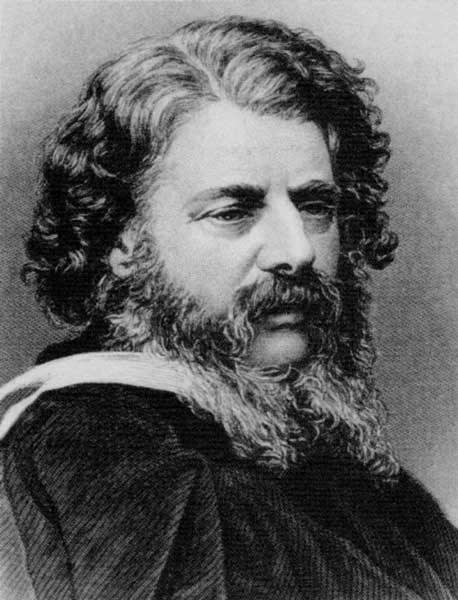
\includegraphics[width=\linewidth]{WilliamRankine.jpg}
  \caption{William Racine had boss facial hair.}
  \label{fig:marginfig}
\end{marginfigure}

\newthought{Potential energy} is the energy that an object has due to its position in a force field or that a system has due to the configuration of its parts.  Common types include the gravitational potential energy of an object that depends on its vertical position and mass, the elastic potential energy of an extended spring, and the electric potential energy of a charge in an electric field. The SI unit for energy is the Joule.

The term potential energy was introduced by the 19th century Scottish engineer and physicist William Rankine, although it has links to Greek philosopher Aristotle's concept of potentiality.  Work done by a conservative force is associated with a change in potential energy.  Potential energy is undefined up to a constant and therefore not a wholly tangible quantity.  The change in potential energy is a tangible quantity.



\section{Total Mechanical Energy}
\begin{marginfigure}[10pt]%
  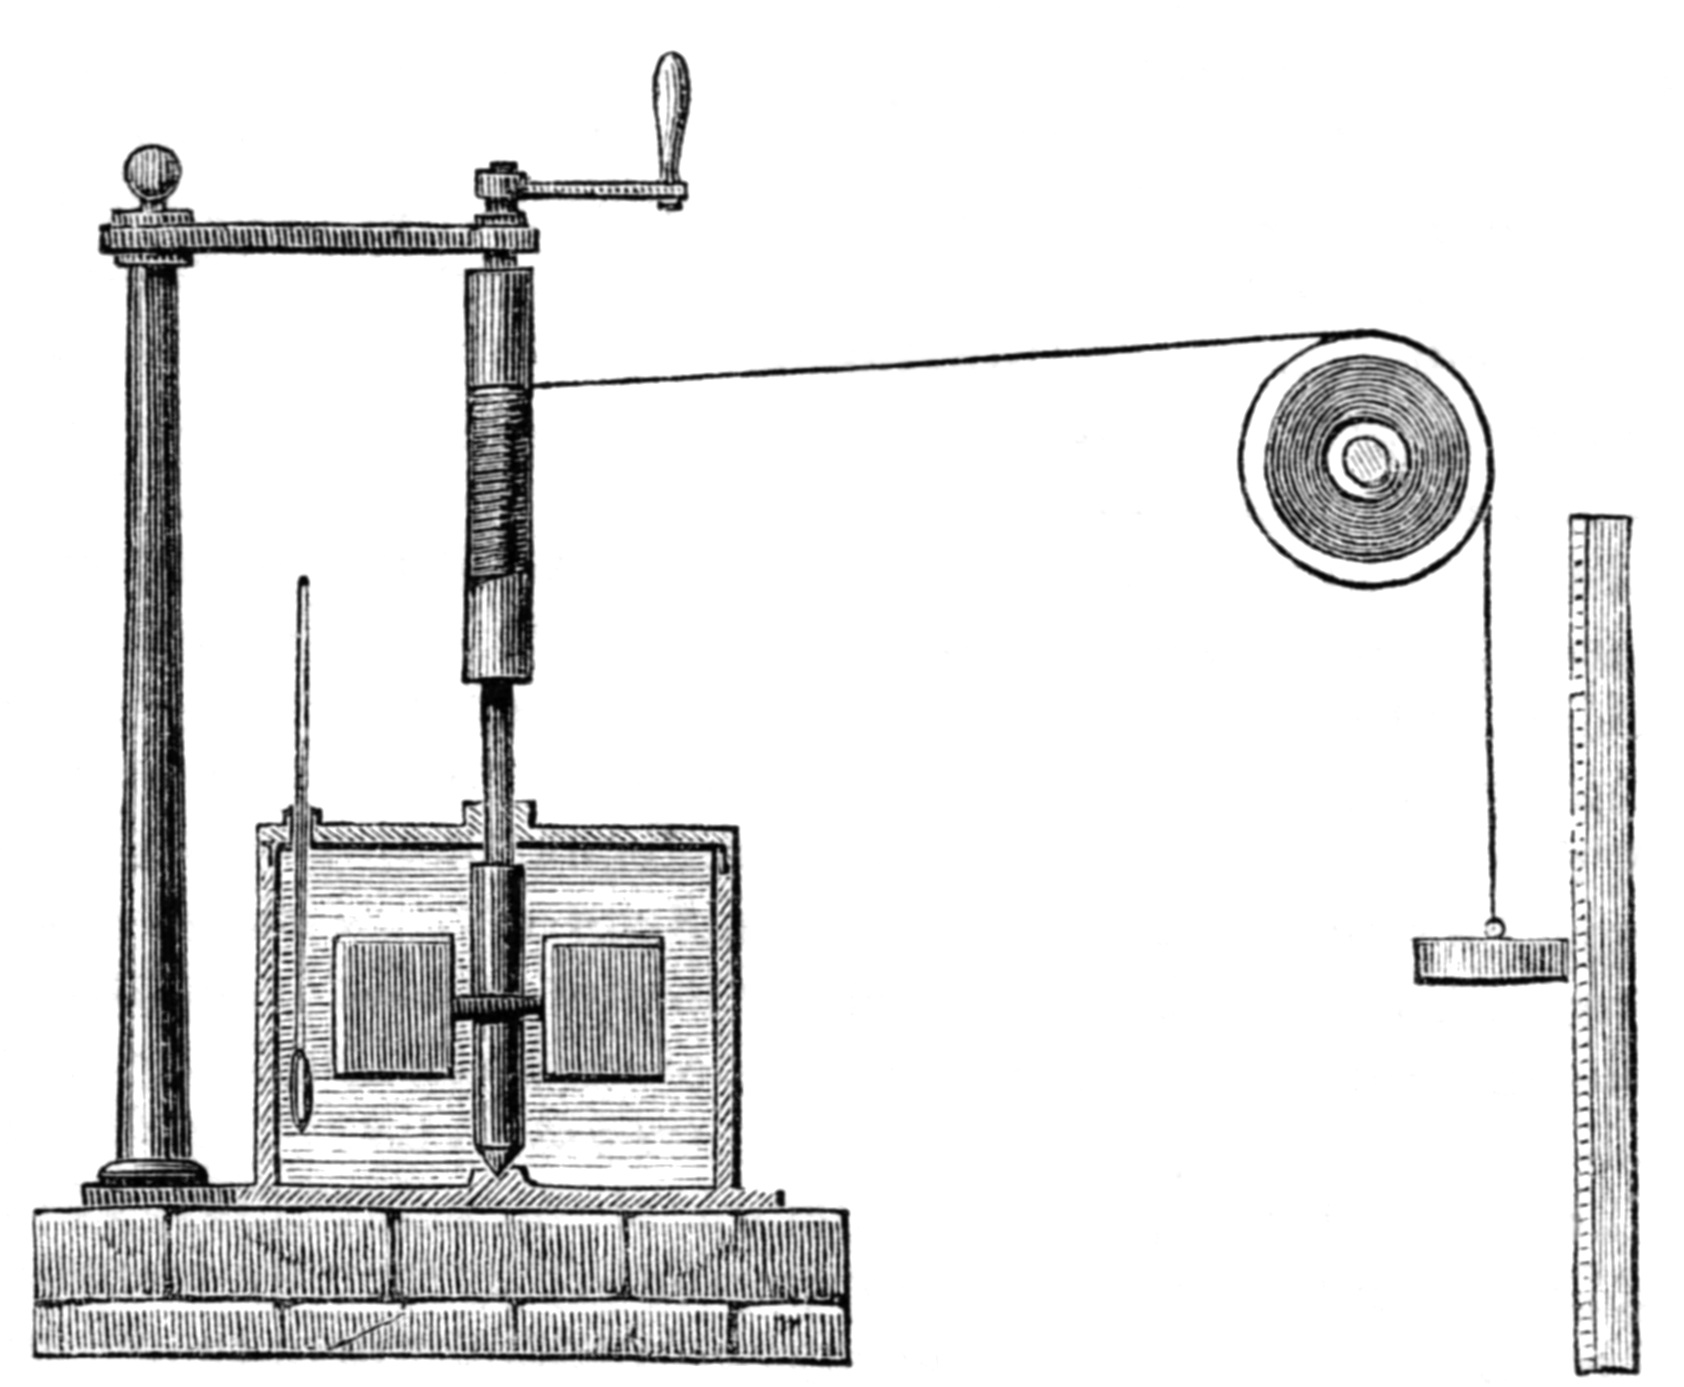
\includegraphics[width=\linewidth]{joule_ap.jpg}
  \caption{Joule's apparatus for measuring the mechanical equivalent of heat.}
  \label{fig:marginfig}
\end{marginfigure}
\newthought{Mechanical energy} is the sum of potential energy and kinetic energy.  The principle of conservation of mechanical energy states that in an isolated system that is only subject to conservative forces the mechanical energy is constant.  In all real systems, however, non-conservative forces, like frictional forces, will be present, but often they are of negligible values and the mechanical energy's being constant can therefore be a useful approximation. In elastic collisions, the mechanical energy is conserved but in inelastic collisions, some mechanical energy is converted into heat. 
$$E=KE+PE$$
$$W_{net}=W_{cons}+W_{non-cons}=\Delta KE$$
$$W_{non-cons}=\Delta{KE}+\Delta{PE}=\Delta(KE+PE)=\Delta{E}$$



\section{Gravitational Work and Potential Energy}
\marginnote[0pt]{Near the surface of the earth the force of gravity on a mass is a relatively constant weight, $mg$.  The potential energy associated with this constant force is the product of weight and displacement.  Note that the physicist chooses where the zero of potential energy is located. }
$$\overrightarrow{F}_g=-mg\hat{y}$$
$$W_g=-mg\ \Delta y$$
$$\Delta PE=-W_g=mg\ \Delta y$$
$$PE=mgy+\cancel{C}=mgy$$

\section{Spring Work and Potential Energy}
\marginnote[0pt]{For an ideal spring the resting force is Hookean.  In this case the potential energy is associated with the area of a triangle, 1/2 base $\times$ height.  The position of zero potential energy is typically taken as the equilibrium position.}
$$\overrightarrow{F}_k=-kx\hat{x}$$
$$W_k=-\frac{k(\Delta x)^2}{2}$$
$$\Delta PE=-W_k=\frac{k(\Delta x)^2}{2}$$
$$PE=\frac{kx^2}{2}+\cancel{C}=\frac{kx^2}{2}$$

\section{Universal Gravitational Work and Potential Energy}
\marginnote[0pt]{The potential energy associated with Newton's universal law of gravitation may seem strange at first glance.  It is negative, which might be confusing.  Verify the PE increases as a mass is moved father from the center of the earth.  Also note the position of zero potential energy is taken to be at infinity.}
$$\overrightarrow{F}_{g}=-\frac{Gm_1m_2}{r^2}\hat{r}$$
$$\Delta PE=-W_g=-\frac{Gm_1m_2}{r}$$
$$PE=-\frac{Gm_1m_2}{r}+\cancel{C}=-\frac{Gm_1m_2}{r}$$
\section{Frictional Work}
\marginnote[0pt]{Friction does not have a potential energy associated with it since it is a non-conservative force.  It is possible however to calculate the work done by friction.  The work done by friction ends up as heat energy.}
$$\overrightarrow{F}_{f}=-\mu_kF_n\hat{v}$$
$$W_f=\overrightarrow{F}_f\cdot \Delta \overrightarrow{r}$$
$$W_f=-\mu_k F_n\ \Delta x$$

Friction is a non-conservative force.

\section{Positive Work / Negative Work / No Work}
\begin{itemize}
  \item Positive Work- (Increases KE/speed) 
  \item Negative Work- (Decreases KE/speed)
  \item No Work- (KE/speed constant)
  \end{itemize}

\marginnote{
  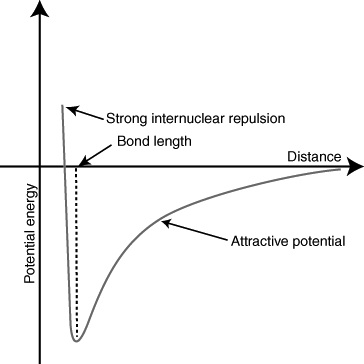
\includegraphics[width=\linewidth ]{peplot.jpg}}
  
  
  \section{Energy Diagrams}
  \begin{itemize}
  \item Potential Energy Wells
  \item  $E$, $PE(x)$, $KE(x)$
  \item Turning Points $KE(x_{turn})=0$
  \item Escape Energy and Escape Velocity
  \end{itemize}
 
\chapter{Momentum}

\begin{marginfigure}%
  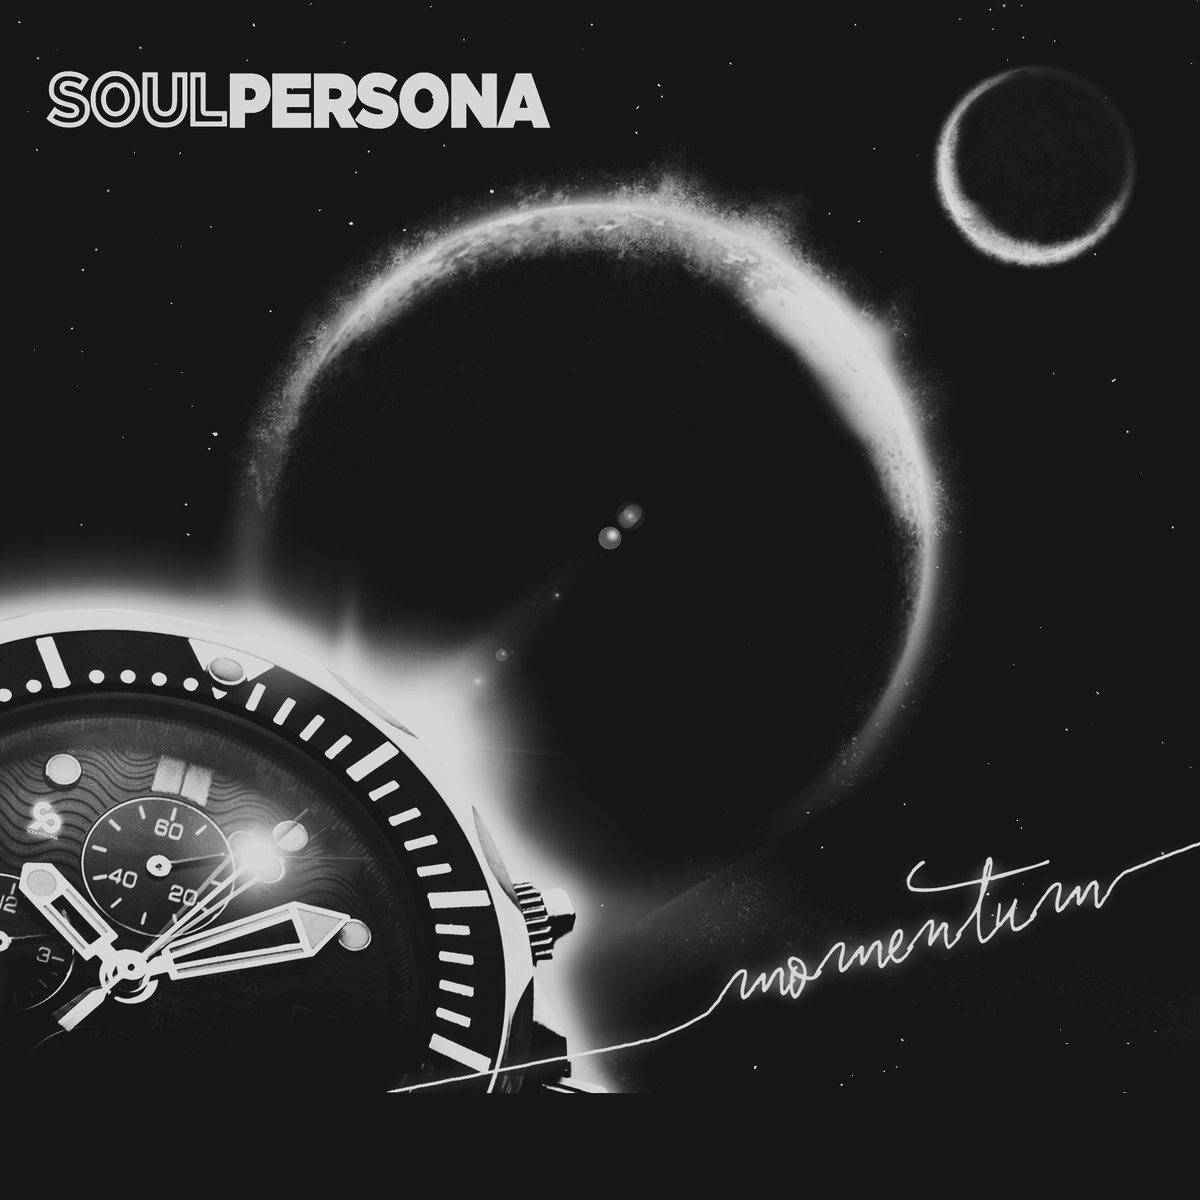
\includegraphics[width=\linewidth]{momentum.jpg}
  \caption{Soul Persona released the hot single \textit{Momentum} in October of 2015.  It's mediocre R\&B synth-pop with great album art.}
  \label{fig:marginfig}
\end{marginfigure}
\textit{Confusion is the beginning of wisdom.}  \\
\noindent\textbf{-   Socrates}


\section{Force, Momentum, Impulse}

\newthought{In classical mechanics}, translational momentum is the product of the mass and velocity of an object.  Since velocity is a vector quantity, momentum is also a vector quantity.
$$\overrightarrow{p}=m\overrightarrow{v}$$

For example, a heavy spaceship moving rapidly has a large momentum.  It takes a large or prolonged force to get the spaceship up to this speed, and it takes a large or prolonged force to bring it to a stop afterwards. If the truck were less massive, or moving more slowly, then it would have less momentum.


\vspace{1cm}

The net force on an object is the time rate of change of the momentum.  This is an alternate representation of Newton's second law.

$$\overrightarrow{F}_{net}=m\overrightarrow{a}=\lim_{\Delta \rightarrow 0}\frac{\Delta \overrightarrow{p}}{\Delta t}$$
$$\left<\overrightarrow{F}_{net}\right>=\frac{\Delta\overrightarrow{p}}{\Delta t}$$

\newthought{Impulse} is the accumulated effect of a force over time.  It is also the change in momentum.  Impulse is also a vector quantity.  Graphically, impulse is the area beneath the $F_{net}(t)$ graph.
$$\overrightarrow{J}=\Delta \overrightarrow{p}=\text{Area}\left( \overrightarrow{F}_{net}(t)\right)$$



\begin{marginfigure}[-200pt]%
\pgfmathdeclarefunction{gauss}{2}{%
  \pgfmathparse{1/(#2*sqrt(2*pi))*exp(-((x-#1)^2)/(2*#2^2))}%
}

\begin{tikzpicture}
    [line cap=round,line join=round,x=2cm,y=2cm, scale=1.2, decoration={brace,amplitude=2pt}]
%main layer
%creating the ticks and xy-axis nodes
%some function
\fill[fill=cyan!20] (0.25,0) -- plot [domain=0.25:1.75] (\x,{2/(sqrt(2*pi))*exp(-((\x-1)^2)/(2*0.2^2))}) -- plot [domain=0.75: 0.25] (\x,0) -- cycle;

 \draw[smooth,samples=200,domain=0:2]
                                 plot(\x,{2/(sqrt(2*pi))*exp(-((\x-1)^2)/(2*0.2^2))});
 

    \fill[black] (0.25,0) circle (0.3mm) node [anchor=north ,scale=1] {$ t_i$};
     \fill[black] (1.75,0) circle (0.3mm) node [anchor=north ,scale=1] {$t_f$};
      %  \fill[black] (0,0.25) circle (0.3mm) node [anchor=south east,scale=1] {\scriptsize$ v(0)$};

  \draw[-latex,color=black,thin] (-0.2,0) -- (2,0) node [anchor=north ,scale=1] {$t$};
   \draw[-latex,color=black,thin] (0,-0.2) -- (0,1.4)node [anchor=east ,scale=1] {$F$};
    \draw (0.6,0.9) node [anchor=south west ,scale=1] {$F_{net}(t)$};
        \draw (1,0.35) node [anchor=center ,scale=1] {$\Delta p$};
         \draw[<->,color=black,thin] (0.25,-0.2) -- (1.75,-0.2)node [midway,anchor=south ,scale=1] {$\Delta t$};
        
 \end{tikzpicture}
  \caption{Impulse is the area under the curve in a force versus time graph.}
  \label{fig:marginfig}
\end{marginfigure}



\newpage

\begin{marginfigure}[40pt]%
  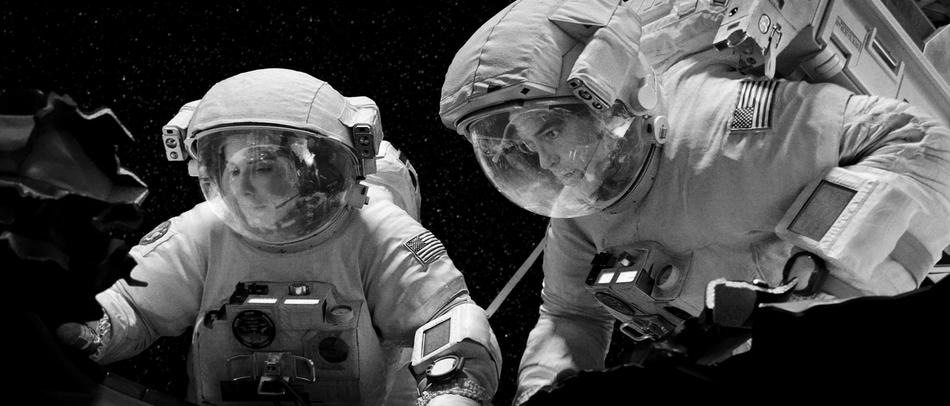
\includegraphics[width=\linewidth]{astronauts.jpg}
  \caption{Two astronauts in deep space are good examples of a system with no external forces.  The total momentum of the two astronauts is conserved unless the earth exerts an external gravitational force or George Clooney fires his thruster.   }
  \label{fig:marginfig}
\end{marginfigure}

\section{Conservation of Momentum}
\newthought{Total momentum is constant} in a closed system, one that does not exchange any matter with its surroundings and is not acted on by external forces. This fact, known as the law of conservation of momentum, is implied by Newton's laws of motion.

Start with Newton's third law.
$$\overrightarrow{F}_{12}=-\overrightarrow{F}_{21}$$
If there are no external forces then the force of particle one on particle two is the net force on particle two and the force of particle two on particle one is the net force on particle two.  
$$\overrightarrow{F}_{2net}=-\overrightarrow{F}_{1net}$$
Next we invoke Newton's second law.
$$\frac{\Delta \overrightarrow{p}_{2}}{\Delta t}=-\frac{\Delta \overrightarrow{p}_{1}}{\Delta t}$$
$$\Delta \overrightarrow{p}_{2}=-\Delta \overrightarrow{p}_{1}$$
Next substitute the definition of what $\Delta p$ is.
$$\overrightarrow{p}_{2f} -\overrightarrow{p}_{2i}=-\overrightarrow{p}_{1f} +\overrightarrow{p}_{1i}$$
Finally separate the terms with final states of the left and initial states on the right.
$$\overrightarrow{p}_{2f} +\overrightarrow{p}_{1f}=\overrightarrow{p}_{1i} +\overrightarrow{p}_{2i}$$
This delivers the conservation of momentum, namely the total momentum of the system is conserved from the initial state to the final state.
$$\overrightarrow{P}_{f}=\overrightarrow{P}_{i} $$

\subsection{External Forces}
In the case of non-zero external forces on the system the total momentum of the system is not conserved.   
$$\sum{ \overrightarrow{F}_{ext}}=M\overrightarrow{a}_{cm}=\lim_{\Delta \rightarrow 0}\frac{\Delta \overrightarrow{P}}{\Delta t}$$

\newpage

\section{Moments, Centroids and Their Time Derivatives  }

\begin{marginfigure}[0pt]%
  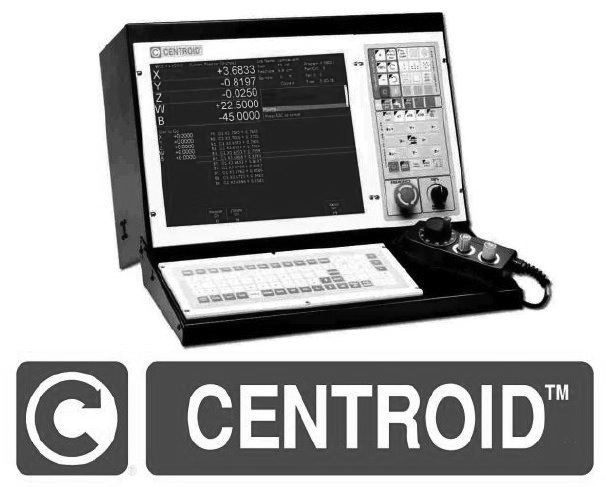
\includegraphics[width=\linewidth]{centroid.jpg}
  \caption{Moments analysis is a general type of statistical analysis. }
  \label{fig:marginfig}
\end{marginfigure}

\newthought{A moment is} a specific quantitative measure describing the distribution of some set of points.  Moments are used in both mechanics and statistics.  If the points represent mass, then the zeroth moment is the total mass, the first moment divided by the total mass is the center of mass, and the second moment is the rotational inertia. If the points represent probability density, then the zeroth moment is the total probability (i.e. one), the first moment is the mean, the second moment is the variance.  

A centroid is another name for the center of mass.  The time rate of change of the first moment is the total momentum.  The time rate of change of the center of mass is also called the velocity of the center of mass.  It is the total momentum divided by the total mass.

\vspace{1cm}

\begin{fullwidth}
\begin{minipage}{7.5cm}
\subsection{2 Particles}
$$M=m_1+m_2$$

$$\overrightarrow{\mathcal{M}_{I}}=m_1\overrightarrow{r}_1+m_2\overrightarrow{r}_2 $$

$$\overrightarrow{P}=\lim_{\Delta \rightarrow 0}\frac{\Delta \overrightarrow{\mathcal{M}_{I}}}{\Delta t}=m_1\overrightarrow{v}_1+m_2\overrightarrow{v}_2$$

$$\overrightarrow{r}_{cm}=\frac{\overrightarrow{\mathcal{M}_{I}}}{M}=\frac{m_1\overrightarrow{r}_1+m_2\overrightarrow{r}_2}{m_1+m_2}$$

$$\overrightarrow{v}_{cm}=\lim_{\Delta \rightarrow 0}\frac{\Delta \overrightarrow{r}_{cm}}{\Delta t}=\frac{m_1\overrightarrow{v}_1+m_2\overrightarrow{v}_2}{m_1+m_2}$$
\end{minipage}
\begin{minipage}{7.5cm}
\subsection{N Particles}

$$M=\sum^N_{n=1}m_n$$

$$\overrightarrow{\mathcal{M}_{I}}=\sum^N_{n=1}m_n\overrightarrow{r}_n$$

$$\overrightarrow{P}=\sum^N_{n=1} m_n\overrightarrow{v}_n$$


$$\overrightarrow{r}_{cm}=\frac{\overrightarrow{\mathcal{M}_{I}}}{M}$$

$$\overrightarrow{v}_{cm}=\frac{\overrightarrow{P}}{M}$$


\end{minipage}



\end{fullwidth}

\vspace{0.5cm}

\begin{figure}
  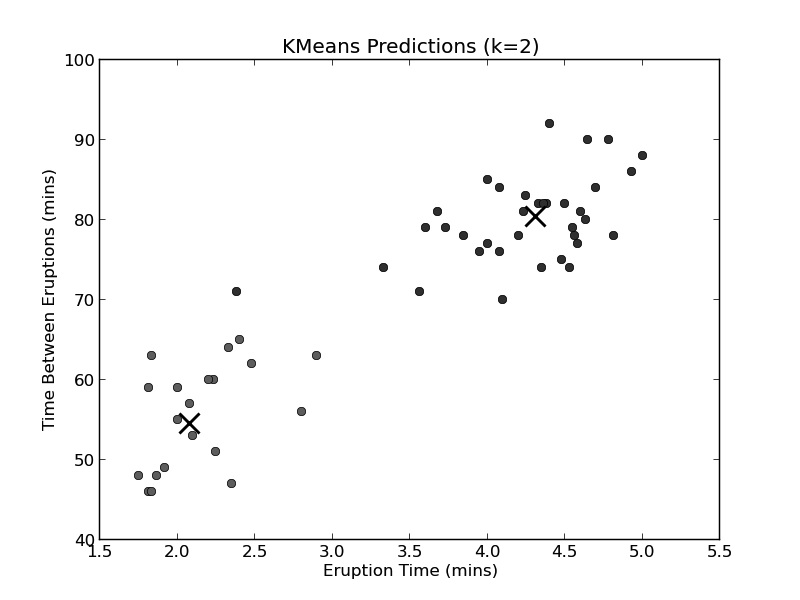
\includegraphics[width=7cm]{centroids.jpg}
  \caption{Each cluster of points in this graph is assigned a centroid.  It represents the average position of the points in each cluster. }
  \label{fig:marginfig}
\end{figure}


\newpage
\section{Collisons}

\begin{marginfigure}
  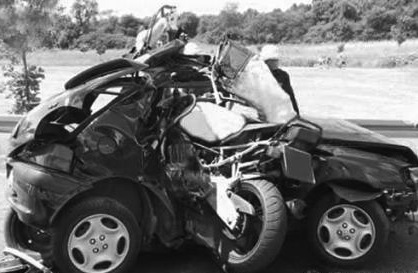
\includegraphics[width=\linewidth]{inelastic.jpg}
  \caption{These are the remnants of an inelastic collision between a car and a motorcycle. }
  \label{fig:marginfig}
\end{marginfigure}

\newthought{A collision} is an event in which two or more bodies exert forces on each other for a relatively short time. Collision implies nothing about the magnitude of the forces.


$$\begin{tikzpicture}[scale=1]
     	
	%\fill[black] (-7,0) circle (0.5mm);   
	%\draw[->,thick] (-7,0) -- (-6,0) node [anchor=west ,scale=1] {$F_g$}; 
	%\fill[black] (7,0) circle (0.5mm);   
%	\draw[->,thick] (7,0) -- (6,0) node [anchor=east ,scale=1] {$F_g$}; 
	 \draw[very thick] (-3,0) circle (0.5cm) node {$m_1$};
	 \draw[->,thick] (-2.5,0) -- (-1.5,0) node [anchor=south, midway ,scale=1] {$\overrightarrow{v}_{1i}$};
	  \draw[very thick] (3,0) circle (0.5cm) node {$m_2$};
	   \draw[->,thick] (2.5,0) -- (1.5,0) node [anchor=south, midway ,scale=1] {$\overrightarrow{v}_{2i}$};
	  %  \draw[thick, color=gray,->] (-4,-0.75) --   (4,-0.75) node [midway, anchor=south] {$r$};
	     
	     
	  %     \begin{scope}[shift={(-3,0)}, scale=0.75] 
	 
	   %\draw[thick](0.2,0.1) -- (0.2,-0.1);
	   % \draw[ thick,-stealth] (0.1,0) -- (1,0) node [near start,anchor=north]{\scriptsize $r$};  
	  %\end{scope}
   
	     
   \end{tikzpicture}$$
   $$\textbf{COLLISION!!!}$$
   $$\begin{tikzpicture}[scale=1]
     	
	%\fill[black] (-7,0) circle (0.5mm);   
	%\draw[->,thick] (-7,0) -- (-6,0) node [anchor=west ,scale=1] {$F_g$}; 
	%\fill[black] (7,0) circle (0.5mm);   
%	\draw[->,thick] (7,0) -- (6,0) node [anchor=east ,scale=1] {$F_g$}; 
	 \draw[very thick] (-3,0) circle (0.5cm) node {$m_1$};
	 \draw[->,thick] (-3.5,0) -- (-4.5,0) node [anchor=south, midway ,scale=1] {$\overrightarrow{v}_{1f}$};
	  \draw[very thick] (3,0) circle (0.5cm) node {$m_2$};
	   \draw[->,thick] (3.5,0) -- (4.5,0) node [anchor=south, midway ,scale=1] {$\overrightarrow{v}_{2f}$};
	  %  \draw[thick, color=gray,->] (-4,-0.75) --   (4,-0.75) node [midway, anchor=south] {$r$};
	     
	     
	  %     \begin{scope}[shift={(-3,0)}, scale=0.75] 
	 
	   %\draw[thick](0.2,0.1) -- (0.2,-0.1);
	   % \draw[ thick,-stealth] (0.1,0) -- (1,0) node [near start,anchor=north]{\scriptsize $r$};  
	  %\end{scope}
   
	     
   \end{tikzpicture}$$

\subsection{One Dimensional Collisions}

\subsubsection{Inelastic}
\newthought{Inelastic collisions} end with the two masses sticking together therefore they end with the same final velocity.  Kinetic energy is lost in an inelastic collision.  Heat is produced.  Momentum is conserved.
$$P_f=P_i$$
$$m_1v_{1f}+m_2v_{2f}=m_1v_{1i}+m_2v_{2i}$$
The masses end with the same final velocity.
$$v_{1f}=v_{2f}=v_{f}$$
The final velocity may be calculated directly.
$$v_{f}=\frac{m_1v_{1i}+m_2v_{2i}}{m_1+m_2}$$

$$\begin{tikzpicture}[scale=1]
     	
	%\fill[black] (-7,0) circle (0.5mm);   
	%\draw[->,thick] (-7,0) -- (-6,0) node [anchor=west ,scale=1] {$F_g$}; 
	%\fill[black] (7,0) circle (0.5mm);   
%	\draw[->,thick] (7,0) -- (6,0) node [anchor=east ,scale=1] {$F_g$}; 
	 \draw[very thick] (-3,0) circle (0.5cm) node {$m_1$};
	 \draw[->,thick] (-2.5,0) -- (-1.5,0) node [anchor=south, midway ,scale=1] {$\overrightarrow{v}_{1i}$};
	  \draw[very thick] (3,0) circle (0.5cm) node {$m_2$};
	   \draw[->,thick] (2.5,0) -- (1.5,0) node [anchor=south, midway ,scale=1] {$\overrightarrow{v}_{2i}$};
	  %  \draw[thick, color=gray,->] (-4,-0.75) --   (4,-0.75) node [midway, anchor=south] {$r$};
	     
	     
	  %     \begin{scope}[shift={(-3,0)}, scale=0.75] 
	 
	   %\draw[thick](0.2,0.1) -- (0.2,-0.1);
	   % \draw[ thick,-stealth] (0.1,0) -- (1,0) node [near start,anchor=north]{\scriptsize $r$};  
	  %\end{scope}
   
	     
   \end{tikzpicture}$$
   $$\textbf{CRASH!!!}$$
   \vspace{0.5cm}
   $$\begin{tikzpicture}[scale=1]
     	
	%\fill[black] (-7,0) circle (0.5mm);   
	%\draw[->,thick] (-7,0) -- (-6,0) node [anchor=west ,scale=1] {$F_g$}; 
	%\fill[black] (7,0) circle (0.5mm);   
%	\draw[->,thick] (7,0) -- (6,0) node [anchor=east ,scale=1] {$F_g$}; 
	% \draw[very thick] (-3,0) circle (0.5cm) node {$m_1$};
	 %\draw[->,thick] (-3.5,0) -- (-4.5,0) node [anchor=south, midway ,scale=1] {$\overrightarrow{v}_{1f}$};
	  \draw[very thick] (0,0) circle (0.8cm) node {$m_1+m_2$};
	   \draw[->,thick] (0.8,0) -- (1.8,0) node [anchor=south, midway ,scale=1] {$\overrightarrow{v}_{f}$};
	  %  \draw[thick, color=gray,->] (-4,-0.75) --   (4,-0.75) node [midway, anchor=south] {$r$};
	     
	     
	  %     \begin{scope}[shift={(-3,0)}, scale=0.75] 
	 
	   %\draw[thick](0.2,0.1) -- (0.2,-0.1);
	   % \draw[ thick,-stealth] (0.1,0) -- (1,0) node [near start,anchor=north]{\scriptsize $r$};  
	  %\end{scope}
   
	     
   \end{tikzpicture}$$
   
   \newpage
   
   \subsubsection{Elastic Collisions}
   \newthought{Elastic collisions} end with both particles bouncing off each other with no loss of kinetic energy.  Both kinetic energy and momentum are conserved during an elastic collision. 
   $$P_f=P_i$$
$$KE_f=KE_i$$
In order to find the final states of the masses the following equations must be solved simultaneously.
$$m_1v_{1f}+m_2v_{2f}=m_1v_{1i}+m_2v_{2i}$$
$$m_1v_{1f}^2+m_2v_{2f}^2=m_1v_{1i}^2+m_2v_{2i}^2$$

$$\begin{tikzpicture}[scale=1]
	 \draw[very thick] (-3,0) circle (0.5cm) node {$m_1$};
	 \draw[->,thick] (-2.5,0) -- (-1.5,0) node [anchor=south, midway ,scale=1] {$\overrightarrow{v}_{1i}$};
	  \draw[very thick] (3,0) circle (0.5cm) node {$m_2$};
	   \draw[->,thick] (2.5,0) -- (1.5,0) node [anchor=south, midway ,scale=1] {$\overrightarrow{v}_{2i}$};
   \end{tikzpicture}$$
   $$\textbf{BOING!!!}$$
   $$\begin{tikzpicture}[scale=1]
	 \draw[very thick] (-3,0) circle (0.5cm) node {$m_1$};
	 \draw[->,thick] (-3.5,0) -- (-4.5,0) node [anchor=south, midway ,scale=1] {$\overrightarrow{v}_{1f}$};
	  \draw[very thick] (3,0) circle (0.5cm) node {$m_2$};
	   \draw[->,thick] (3.5,0) -- (4.5,0) node [anchor=south, midway ,scale=1] {$\overrightarrow{v}_{2f}$};
   \end{tikzpicture}$$


\section{Center of Mass Coordinates}
\newthought{A center of mass coordinate system} shifts the frame of reference to that of the velocity of the center of mass.  The velocities of the masses are calculated relative to the velocity of the center of mass.  An underscore is used to notate velocities which are in the center of mass coordinate system.  

First the velocity of the center of mass is calculated.
$$\overrightarrow{v}_{cm}=\frac{m_1\overrightarrow{v}_1+m_2\overrightarrow{v}_2}{m_1+m_2}$$
Once the velocity of the center of mass is determined the velocities of each mass relative to the center of mass may be calculated.
$$\overrightarrow{\underbar{v}}=\overrightarrow{v}-\overrightarrow{v}_{cm}$$
In a center of mass coordinate system the total momentum of the system is zero.
$$\overrightarrow{\underbar{p}}=m\overrightarrow{\underbar{v}}=m\overrightarrow{v}-m\overrightarrow{v}_{cm}$$
$$\overrightarrow{\underbar{P}}=0$$


\newpage
\section{1-D Collisions}
\marginnote[0pt]{Trucking, tracking, dollying and crabbing are all terms for the technique of putting a camera on a platform (dolly) that slides along a track.  In trucking the camera moves side to side, perpendicular its optical axis.}
\vspace{1cm}
\subsection{Inelastic}
For an inelastic collision the final velocity of the masses is the velocity of the center of mass.
$$\underbar{P}_f=\underbar{P}_i=0$$
$$\underbar{v}_{1f}=\underbar{v}_{2f}=0$$
$$v_{1f}=v_{2f}=v_{cm}$$

\begin{marginfigure}
  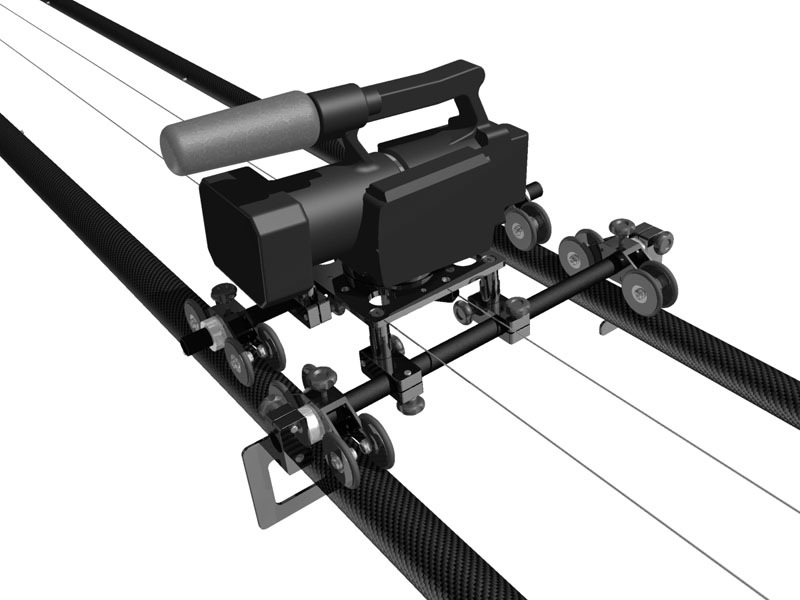
\includegraphics[width=\linewidth]{track.jpg}
  \caption{Center of mass coordinates are tracking shots of which make the total momentum of the system zero. }
  \label{fig:marginfig}
\end{marginfigure}

$$\begin{tikzpicture}[scale=1]
	 \draw[very thick] (-3,0) circle (0.5cm) node {$m_1$};
	 \draw[->,thick] (-2.5,0) -- (-1.5,0) node [anchor=south, midway ,scale=1] {$\overrightarrow{v}_{1i}$};
	  \draw[very thick] (3,0) circle (0.5cm) node {$m_2$};
	   \draw[->,thick] (2.5,0) -- (1.5,0) node [anchor=south, midway ,scale=1] {$\overrightarrow{v}_{2i}$};
   \end{tikzpicture}$$
   
   $$\begin{tikzpicture}[scale=1]
   \draw[dashed,thick] (-5,-1) -- (5,-1) -- (5,1) -- (-5,1) -- (-5,-1);
	 \draw[very thick] (-3,0) circle (0.5cm) node {$m_1$};
	  \draw[->,thick] (5,0) -- (6,0) node [anchor=south, midway ,scale=1] {$\overrightarrow{v}_{cm}$};
	  \draw[->,thick,color=white] (-5,0) -- (-5.5,0);
	 \draw[->,thick] (-2.5,0) -- (-1.5,0) node [anchor=south, midway ,scale=1] {$\overrightarrow{\underbar{v}}_{1i}$};
	  \draw[very thick] (3,0) circle (0.5cm) node {$m_2$};
	   \draw[->,thick] (2.5,0) -- (1.5,0) node [anchor=south, midway ,scale=1] {$\overrightarrow{\underbar{v}}_{2i}$};
   \end{tikzpicture}$$
   
   $$\textbf{CRASH!!!}$$
   
   $$\begin{tikzpicture}[scale=1]
    \draw[dashed,thick] (-5,-1) -- (5,-1) -- (5,1) -- (-5,1) -- (-5,-1);
      \draw[->,thick] (5,0) -- (6,0) node [anchor=south, midway ,scale=1] {$\overrightarrow{v}_{cm}$};
      \draw[->,thick,color=white] (-5,0) -- (-5.5,0);
	 \draw[very thick] (0,0) circle (0.8cm) node {$m_1+m_2$};
   \end{tikzpicture}$$
   
 $$\begin{tikzpicture}[scale=1]
	  \draw[very thick] (0,0) circle (0.8cm) node {$m_1+m_2$};
	   \draw[->,thick] (0.8,0) -- (1.8,0) node [anchor=south, midway ,scale=1] {$\overrightarrow{v}_{cm}$};	
	    \draw[->,thick,color=white] (-0.8,0) -- (-1.8,0) node [anchor=south, midway ,scale=1] {$\overrightarrow{v}_{cm}$};	     
   \end{tikzpicture}$$

\newpage

\subsection{Elastic}
Here is where one gets their money's worth for using center of mass coordinates.  Begin with conservation of momentum and kinetic energy.
$$\underbar{P}_f=\underbar{P}_i=0$$
$$\underbar{KE}_f=\underbar{KE}_i$$
Calculate the center of mass velocity.
$$\overrightarrow{v}_{cm}=\frac{m_1\overrightarrow{v}_1+m_2\overrightarrow{v}_2}{m_1+m_2}$$
Next determine the velocity of each mass in the center of mass velocity frame.
$$\underbar{v}_{1i}={v}_{1i}-v_{cm} \hspace{1cm} \underbar{v}_{2i}={v}_{2i}-v_{cm}$$
In the center of mass coordinate system the masses simply switch direction after collision.  This is the only way to maintain zero momentum and conserve kinetic energy.
$$\underbar{v}_{1f}=-\underbar{v}_{1i} \hspace{1cm} \underbar{v}_{2f}=-\underbar{v}_{2i}$$
Finally convert back to the original coordinate system.
$$v_{1f}=2v_{cm}-v_{1i} \hspace{1cm} v_{2f}=2v_{cm}-v_{2i}$$

$$\begin{tikzpicture}[scale=1]
	 \draw[very thick] (-3,0) circle (0.5cm) node {$m_1$};
	 \draw[->,thick] (-2.5,0) -- (-1.5,0) node [anchor=south, midway ,scale=1] {$\overrightarrow{v}_{1i}$};
	  \draw[very thick] (3,0) circle (0.5cm) node {$m_2$};
	   \draw[->,thick] (2.5,0) -- (1.5,0) node [anchor=south, midway ,scale=1] {$\overrightarrow{v}_{2i}$};
   \end{tikzpicture}$$
   
   $$\begin{tikzpicture}[scale=1]
   \draw[dashed,thick] (-5,-1) -- (5,-1) -- (5,1) -- (-5,1) -- (-5,-1);
	 \draw[very thick] (-3,0) circle (0.5cm) node {$m_1$};
	  \draw[->,thick] (5,0) -- (6,0) node [anchor=south, midway ,scale=1] {$\overrightarrow{v}_{cm}$};
	  \draw[->,thick,color=white] (-5,0) -- (-5.5,0);
	 \draw[->,thick] (-2.5,0) -- (-1.5,0) node [anchor=south, midway ,scale=1] {$\overrightarrow{\underbar{v}}_{1i}$};
	  \draw[very thick] (3,0) circle (0.5cm) node {$m_2$};
	   \draw[->,thick] (2.5,0) -- (1.5,0) node [anchor=south, midway ,scale=1] {$\overrightarrow{\underbar{v}}_{2i}$};
   \end{tikzpicture}$$
   
   $$\textbf{BOING!!!}$$
   
   $$\begin{tikzpicture}[scale=1]
    \draw[dashed,thick] (-5,-1) -- (5,-1) -- (5,1) -- (-5,1) -- (-5,-1);
      \draw[->,thick] (5,0) -- (6,0) node [anchor=south, midway ,scale=1] {$\overrightarrow{v}_{cm}$};
      \draw[->,thick,color=white] (-5,0) -- (-5.5,0);
	 \draw[very thick] (-3,0) circle (0.5cm) node {$m_1$};
	 \draw[->,thick] (-3.5,0) -- (-4.5,0) node [anchor=south, midway ,scale=1] {$-\overrightarrow{\underbar{v}}_{1i}$};
	  \draw[very thick] (3,0) circle (0.5cm) node {$m_2$};
	   \draw[->,thick] (3.5,0) -- (4.5,0) node [anchor=south, midway ,scale=1] {$-\overrightarrow{\underbar{v}}_{2i}$};

   \end{tikzpicture}$$
   
    $$\begin{tikzpicture}[scale=1]
    %\draw[dashed,thick] (-5,-1) -- (5,-1) -- (5,1) -- (-5,1) -- (-5,-1);
     % \draw[->,thick] (5,0) -- (6,0) node [anchor=south, midway ,scale=1] {$\overrightarrow{v}_{cm}$};
      %\draw[->,thick,color=white] (-5,0) -- (-5.5,0);
	 \draw[very thick] (-3,0) circle (0.5cm) node {$m_1$};
	 \draw[->,thick] (-3.5,0) -- (-4.5,0) node [anchor=south ,scale=1] {\small$-\overrightarrow{\underbar{v}}_{1i}+\overrightarrow{v}_{cm}$};
	  \draw[very thick] (3,0) circle (0.5cm) node {$m_2$};
	   \draw[->,thick] (3.5,0) -- (4.5,0) node [anchor=south ,scale=1] {\small$-\overrightarrow{\underbar{v}}_{2i}+\overrightarrow{v}_{cm}$};

   \end{tikzpicture}$$

 
\chapter{Rotational Dynamics}

\begin{marginfigure}%
  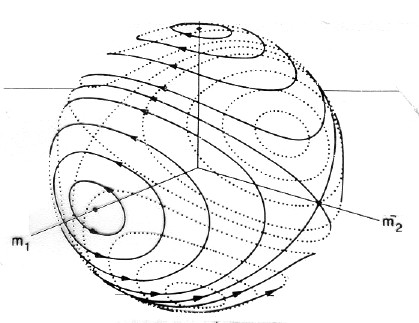
\includegraphics[width=\linewidth]{rigidbody.jpg}
  \caption{Phase portrait of the free rigid body, such as a hammer tossed in the air.}
  \label{fig:marginfig}
\end{marginfigure}


\textit{The Harley's got a little too much torque.}  \\
\noindent\textbf{-   Evel Knievel}


 \section{Rigid Bodies}
 A rigid body is an idealization of a solid body in which deformation is neglected. In other words, the distance between any two given points of a rigid body remains constant in time regardless of external forces exerted on it.  A rigid body is considered to be non-deformable.
 
 \marginnote{Rigidity is a quality found in people and objects that don't bend, though they might eventually break. When we see rigidity in a person, it means they're severe, like a teacher who punishes you for being late even though you were busing saving an orphan from a polar bear.}
 
 
 \section{Torque}
 Torque, moment, or moment of force is the tendency of a force to rotate an object about an axis, fulcrum, or pivot. Just as a force is a push or a pull, a torque can be thought of as a twist to an object. Mathematically, torque is defined as the cross product of the lever-arm distance vector and the force vector, which tends to produce rotation.
  $$\overrightarrow{\tau}\equiv \overrightarrow{r}\times  \overrightarrow{F}$$
  %$$\overrightarrow{\tau}=\lim_{\Delta \rightarrow 0}\frac{\Delta \overrightarrow{l}}{\Delta t}$$
%\vspace{0.1cm}

\section{Newton's First Law for Rigid Bodies}
$$\sum{ \overrightarrow{F}_{ext}}=0 \ \ \longleftrightarrow \ \ \overrightarrow{a}=0 $$
$$\sum{ \overrightarrow{\tau}_{ext}}=0 \ \ \longleftrightarrow \ \ \overrightarrow{\alpha}=0$$ \ \ \ \ \ \marginnote{Torques may be applied around any axis.  Torques, in general, have no meaning without an indication of where they are calculated with respect to.}


 \section{Statics}
 $$\sum{ \overrightarrow{F}_{ext}}=0$$
  $$\sum{ \overrightarrow{\tau}_{ext}}=0$$
  
  \newpage
  
\section{Newton's Second Law for Rigid Bodies}
Newton's second law for rigid bodies related the total torque to the angular acceleration of the system.  The inertial factor serving as the constant of proportionality is the moment of inertia.
$$\sum{ \overrightarrow{F}_{ext}}=m \overrightarrow{a}$$
$$\sum{ \overrightarrow{\tau}_{ext}}=I \overrightarrow{\alpha}$$
 \vspace{0.1cm}
 
 \section{Pure Moments/Couples}
 A pure moment, or couple, is a set of forces which add to zero but are applied in such a way to give a net torque.  In the case of a couple the net torque can be calculated around any point.  Isn't that neat?  Can you prove that mathematically?
 $$\sum{ \overrightarrow{F}_{ext}}=0$$
  $$\sum{ \overrightarrow{\tau}_{ext}}=I \overrightarrow{\alpha}$$
  \vspace{0.1cm}
  
 \section{Moments of Inertia}
 \vspace{0.1cm}
 \marginnote{Our treatment is in 2-D.  The 3-D treatment requires more complicated mathematical representations and is beyond the scope of an introductory course.}
 Consider a rigid body consisting on $N$ massive particles.  We use an index variable $i$ so that each particle has a mass $m_i$ and a position vector $\overrightarrow{r_i}$.  We define the moment of inertia for rotations around the origin as follows.  It is the sum of the masses "weighted" by their square distance from the axis of rotation.
 \vspace{0.1cm}
$$ I\equiv \sum\limits_{i=1}^{N} r_i^2m_i$$
\vspace{0.1cm}
The moment of inertia depends on the rotational axis it is in reference to.  Moving the axis of rotation to the center of mass minimizes the moment of inertia.  We use an $\underbar{underbar}$ to notate this. 
\vspace{0.1cm}
$$ \underbar{I}=\sum\limits_{i=1}^{N} \underbar{r}_i^2m_i$$
%\vspace{1cm}

 \section{Parallel Axis Theorem}
 Moving the axis of rotation a distance $D$ from the center of mass gives a new moment of intertia.
 \vspace{0.1cm}
 $$ I= \underbar{I}+MD^2$$
 
 \newpage
 
 \section{Example Moments of Inertia}
  \vspace{1cm}
  
 \begin{center}
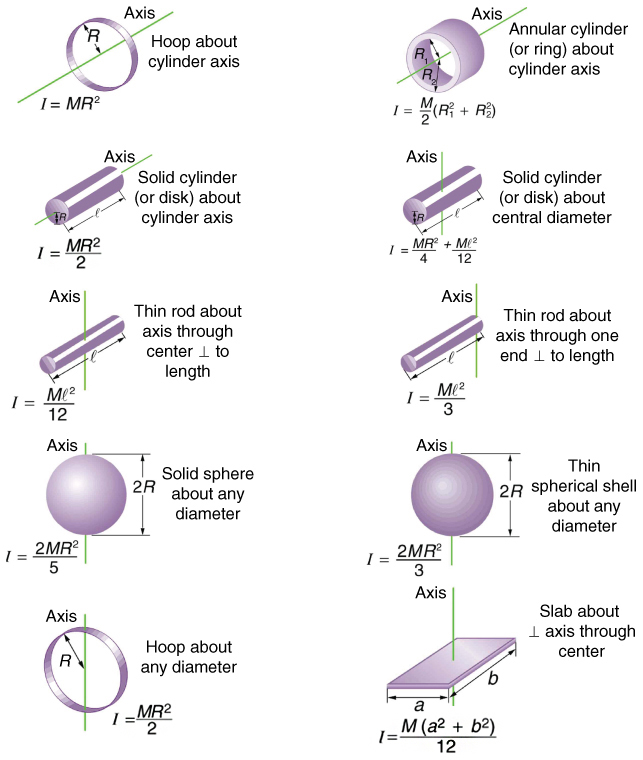
\includegraphics[height=8in,width=6in,angle=0]{moments.jpg}

\end{center}
 
 \section{Torque in Another Light}
 Torque may also be represented as the time rate of change of the angular momentum.
  $$\overrightarrow{\tau}\equiv \overrightarrow{r}\times  \overrightarrow{F}$$
  $$\overrightarrow{\tau}=\frac{d \overrightarrow{l}}{dt}$$
  
\section{Angular Momentum}
Angular momentum s a vector quantity that represents the product of a body's rotational inertia and rotational velocity about a particular axis. In the simple case of revolution of a particle in a circle about a center of rotation, the particle remaining always in the same plane and having always the same distance from the center, it is sufficient to discard the vector nature of angular momentum, and treat it as a scalar.  Angular momentum can be considered a rotational analog of linear momentum. Thus, where linear momentum is proportional to mass and linear speed angular momentum is proportional to moment of inertia and angular speed.

A single particle moves with an angular momentum $\overrightarrow{l}$.
 $$\overrightarrow{l}\equiv \overrightarrow{r}\times  \overrightarrow{p}$$
 \marginnote{The angular momentum, in general, only has meaning in reference to some center point.}
 $$\left|\overrightarrow{l}\right|= \left|\overrightarrow{r}\times  \overrightarrow{p}\right|=mr^2\omega$$
 The total angular momentum for a system of particles is notated $\overrightarrow{L}$.  It is calculated by the sum of the individual particle momenta.
  $$\overrightarrow{L}\equiv \sum_i \overrightarrow{l}_i $$
  Since each particle in a rigid body is moving at the same angular velocity we may represent the total angular momentum as the product of the moment of inertia and the angular velocity.
  \marginnote{The total angular momentum of a system is independent of the location of the reference point if the total linear momentum is equal to zero.  Can you prove that?  Can you choose a frame where the linear total momentum is equal to zero?  Do you see where we are going with this?}
  $$\overrightarrow{L}= \sum_i m_ir_i^2\omega$$
  $$\overrightarrow{L}= I\omega$$

\newpage
  
  \section{Conservation of Angular Momentum}
$$\overrightarrow{r}\times\overrightarrow{F}_{12}=-\overrightarrow{r}\times\overrightarrow{F}_{21}$$
\subsection{No External Torques}
\marginnote{This derivation is almost identical to that for conservation of linear momentum.}
$$\overrightarrow{r}\times\overrightarrow{F}_{2net}=-\overrightarrow{r}\times\overrightarrow{F}_{1net}$$
$$ \overrightarrow{r}\times\overrightarrow{F}_{2net}\ \Delta t=-\overrightarrow{r}\times\overrightarrow{F}_{1net}\ \Delta t$$
$$\Delta \overrightarrow{l}_{2}=-\Delta \overrightarrow{l}_{1}$$
$$\overrightarrow{l}_{2f} -\overrightarrow{l}_{2i}=-\overrightarrow{l}_{1f} +\overrightarrow{l}_{1i}$$
$$\overrightarrow{l}_{2f} +\overrightarrow{l}_{1f}=\overrightarrow{l}_{1i} +\overrightarrow{l}_{2i}$$
$$\overrightarrow{L}_{f}=\overrightarrow{L}_{i} $$
\subsection{External Forces}
\marginnote{If there are external torques they act to change the total angular momentum of the system.}
$$\sum{ \overrightarrow{\tau}_{ext}}=I\overrightarrow{\alpha}=\frac{\Delta\overrightarrow{L}}{\Delta t}$$
 


  \section{Rotational Work and Power}
  \marginnote{ The rotational analogue of work is the dot product between the torque and the angular displacement.  The net rotational work generates a change in rotational kinetic energy.  The time rate of change of the rotational work is the rotational power.}
 $$W_{rot}= \overrightarrow{\tau}\cdot \Delta \overrightarrow{\theta}$$
 $$P_{rot}=\lim_{\Delta\rightarrow 0}\frac{\Delta W_{rot}}{\Delta t}=\overrightarrow{\tau}\cdot \overrightarrow{\omega}$$

 
 \section{Rotational Kinetic Energy}
 $$\sum W_{rot}=\sum \overrightarrow{\tau}\cdot \Delta\overrightarrow{\theta}=\Delta KE_{rot}$$
 $$KE_{rot}=\frac{L^2}{2I}=\frac{I\omega^2}{2}$$
 $$KE=\underbar{KE}_{rot}+KE_{lin}=\frac{\underbar{L}^2}{2\underbar{I}}+\frac{\underbar{P}^2}{2M}=\frac{\underbar{I}\omega^2}{2}+\frac{Mv_{cm}^2}{2}$$

 \section{Rolling}
 \begin{marginfigure}[10pt]
  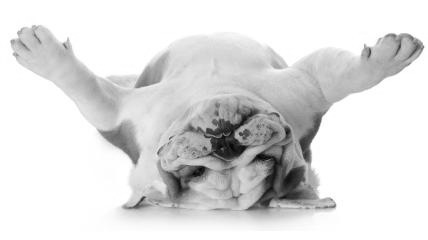
\includegraphics[width=\linewidth]{rolling.jpg}
  \caption{This dog is rolling.}
  \label{fig:marginfig}
\end{marginfigure}
 $$v_{cm}=R\omega$$
 $$a_{cm}=R\alpha$$
 $$KE=\frac{I_p\omega^2}{2}=\frac{\underbar I}{2}\omega^2+\frac{MR^2}{2}\omega^2=\frac{1}{2}\left(\frac{\underbar I}{R^2}+M\right)v_{cm}^2$$
 \section{Precession of a Top}
  \section{Rolling}
 \begin{marginfigure}[10pt]
  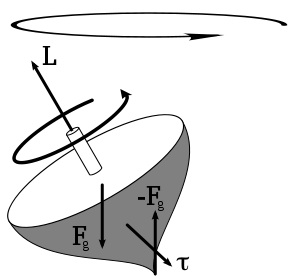
\includegraphics[width=\linewidth]{top.jpg}
  \caption{Precession of a top}
  \label{fig:marginfig}
\end{marginfigure}
 $$\sum{ \overrightarrow{F}_{ext}}=(F_n-Mg)\hat{z}=0$$
 $$\sum{ \overrightarrow{\tau}_{ext}}=\overrightarrow{0}\times(F_n\hat{z})+\overrightarrow{\scriptr}_{cm}\times(-Mg\hat{z})$$
 $$\frac{d\overrightarrow{L}}{dt}=-Mg\overrightarrow{\scriptr}_{cm}\times\hat{z}$$
 Precession is the result of the angular velocity of rotation and the angular velocity produced by the torque. It is an angular velocity about a line that makes an angle with the permanent rotation axis, and this angle lies in a plane at right angles to the plane of the couple producing the torque.  If the rotating body is symmetrical, its motion unconstrained and the torque on the spin axis is at right angles to that axis, the axis of precession will be perpendicular to both the spin axis and torque axis.
 \section{Quantization of Angular Momentum}
 Quantization of angular momentum is one of the deeper mysteries of the universe.  It was first postulated by Niels Bohr in his Bohr model of the atom and was later predicted by Erwin Schrodinger.  Angular momentum must be an integer multiple of the reduced Planck's constant $\hbar$.  The lowest possible angular momentum of a system is the reduced Planck's constant.
$$ L=n\hbar$$
$$ \underbar{I}\omega=n\hbar$$
$$ \hbar=\frac{h}{2\pi}=1.05\times 10^{-34}\  \footnotesize \frac{\text{kg}\cdot \text{m}^2}{\text{s}^2}$$




  
\chapter{Orbits}

\textit{Without proper experiments I conclude nothing.}\\
\noindent\textbf{-   Johannes Kepler}

\begin{marginfigure}%
  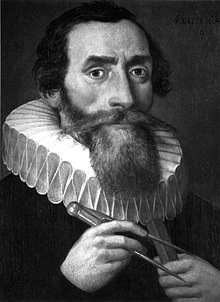
\includegraphics[width=\linewidth]{kepler.jpg}
  \caption{This 1610 portrait shows Kepler, at age 39, with his chopsticks.}
  \label{fig:marginfig}
\end{marginfigure}

\section{History}
Johannes Kepler was a German mathematician, astronomer, and astrologer. A key figure in the 17th century scientific revolution, he is best known for his laws of planetary motion.  His work advanced the Copernican heliocentric model.  From 1600 to 1610 Kepler took over the observational work of Tycho Brahe, publishing star charts in 1627, known as the \textit{Rudolphine Tables}.  In this time Kepler collaborated with Galileo and advanced fundamental optics through development of the refracting telescope.  Kepler provided foundations for Isaac Newton's theory of universal gravitation.

\begin{marginfigure}[100pt]
  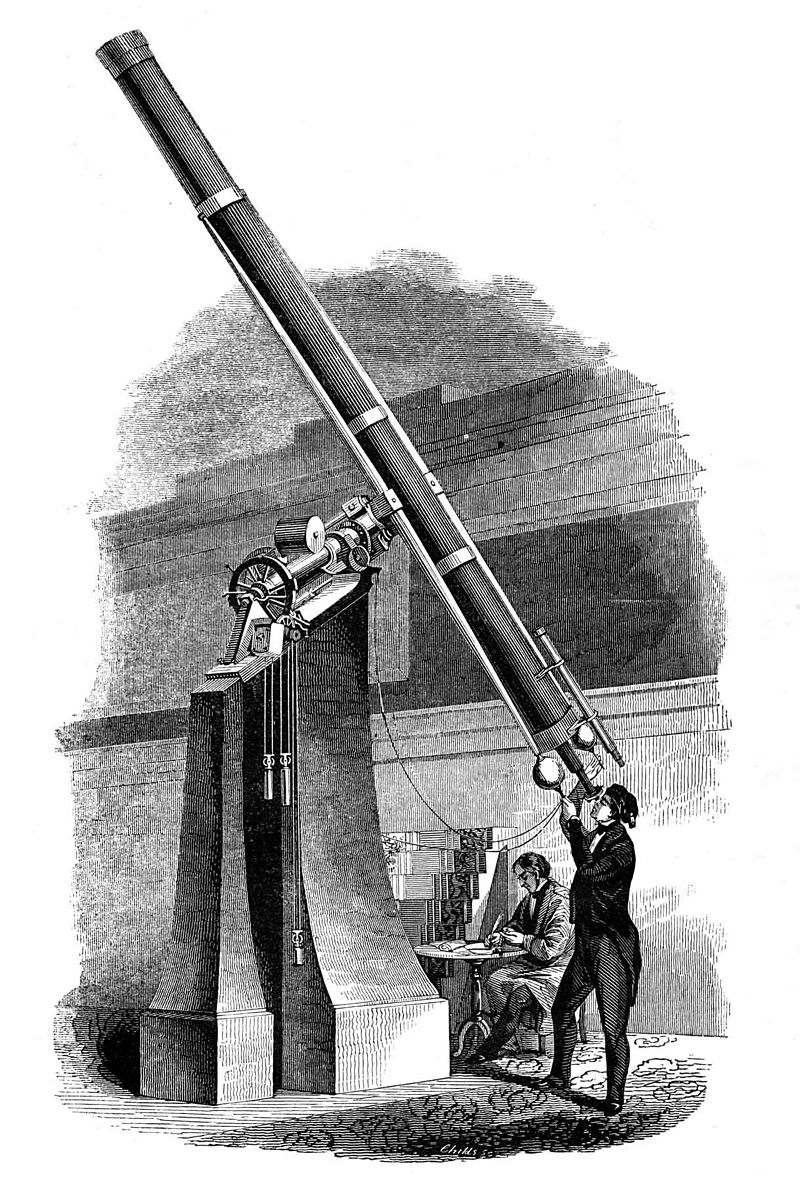
\includegraphics[width=\linewidth]{telescope.jpg}
  \caption{Refracting telescope from the Cincinnati Observatory in 1848.}
  \label{fig:marginfig}
\end{marginfigure}

\section{Kepler's Laws}
Kepler's Laws are three statements describing the motion of planets around the sun.

\begin{enumerate}
\item The orbit of a planet is an ellipse with the Sun at one of the two foci.
\item A line segment joining a planet and the Sun sweeps out equal areas during equal intervals of time.
\item The square of the orbital period of a planet is proportional to the cube of the semi-major axis of its orbit.
\end{enumerate}


\newpage

\section{Circular Orbital Motion}
\vspace{0.5cm}

\subsection{General}

\begin{marginfigure}
\begin{tikzpicture}[scale=0.55]	
\draw [color=gray!80] (0,0)--(3,0) node [midway,anchor=south,inner sep=1pt, outer sep=1pt]{$r$};


\begin{scope}[shift={(0,0)}, scale=1,rotate=120] 
 	\draw[color=gray,dashed] (0,0) circle (3cm);
	
	\begin{scope}[shift={(0,-4)}, scale=0.75, rotate=-90] 
		\draw[ thick,-stealth] (0,-0.1) -- (0,0.8) node [near start,anchor=east]{\scriptsize $\theta$};  
		\draw[thick](-0.1,0) -- (0.1,0);
		\draw[thick](0.2,-0.4) -- (0.2,-0.6);
		\draw[ thick,-stealth] (0.1,-0.5) -- (1,-0.5) node [near start,anchor=north]{\scriptsize $r$};  
	\end{scope}
	
	\fill[black] (0,0) circle (1mm);  
	\fill[color=white] (0.5,-2.5) -- (-0.5,-2.5) -- (-0.5,-3.5) -- (0.5,-3.5) -- cycle;
	\draw[very thick] (0,-3) circle (0.5cm);
 	\draw (0,-3) node {$m$};
 \end{scope}	
 	  
 \begin{scope}[shift={(7,0)}, scale=1,rotate=120] 
 	\draw[->,thick] (0,0) -- (0,1.3) node [anchor=east ,scale=1] {$F_{c}$}; 	 
    	\fill[black] (0,0) circle (0.5mm);   
\end{scope}

\end{tikzpicture}
  \caption{General circular orbit}
  \label{fig:fig}
\end{marginfigure}

The speed in circular orbit is the product of radius and angular velocity.
$$v=\omega r$$
There is some force causing centripetal acceleration.   
$$\overrightarrow{F}_c=-\frac{mv^2}{r}\hat{r}=-m\omega^2r\hat{r}$$
The kinetic energy turns out to be half the product of this force and the radius of orbit.
$$KE=\frac{mv^2}{2}=\frac{F_cr}{2}$$
%$$-\nabla PE= \overrightarrow{F}_c$$





\subsection{Gravity}
For planetary orbits gravity is the force causing centripetal acceleration.  
$$\overrightarrow{F}_c=-\frac{mMG}{r^2}\hat{r}$$
Using Newton's law of universal gravitation, the potential energy is identified.
$$PE=-\frac{mMG}{r}$$
For an circular motion from an inverse square force law, such as that for gravity or electrostatics, the kinetic energy is half the negative potential energy and the total energy is negative and equal in magnitude to the kinetic energy.
 
$$KE=\frac{F_cr}{2}=\frac{mMG}{2r}=-\frac{PE}{2}$$
$$E=-KE$$
\subsubsection{Period of Gravitational Orbit}
\begin{marginfigure}[0pt]
  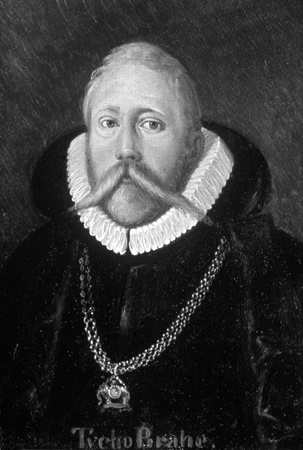
\includegraphics[width=\linewidth]{brahe.jpg}
  \caption{Tycho Brahe was a slick dutchman with a sweet 'stache and a brass nose.}
  \label{fig:marginfig}
\end{marginfigure}
Kepler's third law is easily derived for circular gravitational orbits by equating the centripetal force and the universal gravitational force.
$$m\omega^2r=\frac{mMG}{r^2}$$
This can be used to express the relationship between the period and radius of orbit.
$$T=\frac{2\pi}{\omega}=\sqrt{\frac{4\pi^2 r^3}{MG}}$$


\newpage

\begin{marginfigure}[0pt]
  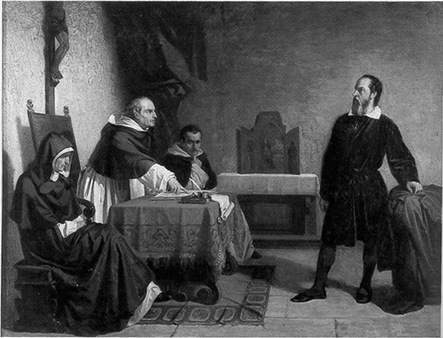
\includegraphics[width=\linewidth]{galileo.jpg}
  
  \caption{Cristiano Banti's 1857 painting \textit{Galileo facing the Roman Inquisition}.}
  \label{fig:marginfig}
\end{marginfigure}
\subsection{Central Spring}
The following represents the situation when the force causing centripetal acceleration is Hookean.  
$$\overrightarrow{F}_c=-kr\hat{r}$$
In this case the potential energy and kinetic energy are equal.
$$PE=\frac{kr^2}{2}$$
$$KE=\frac{F_cr}{2}=\frac{kr^2}{2}=PE$$
$$E=2KE$$
\marginnote{The Hookean centripetal force is of interest because it arises in the case of gravitational attraction to a sphere of uniformly distributed mass.}
\subsubsection{Period of Spring Orbit}
The angular velocity and period of orbit are derived as follows.
$$m\omega^2r=kr$$
$$\omega=\sqrt{\frac{k}{m}}$$
$$T=\frac{2\pi}{\omega}$$


\section{Elliptic Gravitational Orbits}
\subsection{Kepler's First Law}
The orbit of every planet is an ellipse with the Sun at one of the two foci.
\subsubsection{Conservation Laws}
$$E=KE+PE=\frac{mv^2}{2}-\frac{mMG}{r}=\text{constant}$$
$$L=mr^2\omega=\text{constant}$$
\marginnote{A conic section is a curve obtained as the intersection of a cone with a plane.  The eccentricity, e, determines if the conic section is a hyperbola, parabola, ellipse or a circle.  e =  0 the section is a circle.  0<e<1 the section is an ellipse.  e=1, a parabola and e>1 a hyperbola.}
\subsubsection{Conic Sections and Eccentricity}
$$r=\frac{r_0}{1+e\cos{\theta}}$$
$$e^2=1+\frac{2Er_0}{GMm}$$
\vspace{1cm}

\subsection{Kepler's Second Law}
A line joining a planet and the Sun sweeps out equal areas during equal intervals of time.\\ \ \\

In an infinitesimally small length of time, $\Delta t$, the line joining the sun and planet sweeps out an infinitesimally small area, $\Delta A$.
$$\frac{\Delta A}{\Delta t}=\frac{1}{2}r v_{tan}=\frac{1}{2}r^2\omega$$
The rate of change of the swept out area is directly proportional to the angular momentum.
$$\frac{\Delta A}{\Delta t}=\frac{L}{2}$$
Since the angular momentum is constant so is the rate of change of the area.
$$\frac{\Delta A}{\Delta t}=\text{constant}$$

\begin{figure}
$$\begin{tikzpicture}
    [line cap=round,line join=round,x=2cm,y=2cm, scale=1.5, decoration={brace,amplitude=2pt}]
%main layer
%creating the ticks and xy-axis nodes
%some function
\fill[fill=cyan!20] (0,0) -- plot [samples=200,domain=120:140] ({0.5*cos(\x)/(1+0.75*cos(\x))},{0.5*sin(\x)/(1+0.75*cos(\x)}) -- cycle;

 \draw[smooth,samples=200,domain=0:360]
                                 plot({0.5*cos(\x)/(1+0.75*cos(\x))},{0.5*sin(\x)/(1+0.75*cos(\x)});
 
\fill[fill=black!20] plot [samples=3,domain=120:140] ({0.5*cos(\x)/(1+0.75*cos(\x))},{0.5*sin(\x)/(1+0.75*cos(\x)}) circle (0.8mm);


    \fill[black] (0,0) circle (0.8mm) node [anchor=north ,scale=1] {$ $};
     \fill[black] (0,0) circle (0.8mm) node [anchor=north ,scale=1] {$ $};
     %\fill[black] (1.75,0) circle (0.3mm) node [anchor=north ,scale=1] {$t_f$};
      %  \fill[black] (0,0.25) circle (0.3mm) node [anchor=south east,scale=1] {\scriptsize$ v(0)$};

  %\draw[-latex,color=black,thin] (-0.2,0) -- (2,0) node [anchor=north ,scale=1] {$t$};
   %\draw[-latex,color=black,thin] (0,-0.2) -- (0,1.4)node [anchor=east ,scale=1] {$F$};
    \draw (0,0) -- (0,-0.5) node [midway, anchor=east ,scale=0.75] {$r_0$};
      \draw (-0.45,0.5) node [anchor=center,scale=0.75] {\scriptsize $\frac{\Delta A}{\Delta t}\Delta t$};
       \draw (-0.12,0.13) node [anchor=center,scale=0.65] {\scriptsize $\Delta \theta$};
       % \draw (1,0.35) node [anchor=center ,scale=1] {$\Delta p$};
         %\draw[<->,color=black,thin] (0.25,-0.2) -- (1.75,-0.2)node [midway,anchor=south ,scale=1] {$\Delta t$};
        
 \end{tikzpicture}$$
  \caption{Kepler's third law is an outcome of conservation of angular momentum.}
  \label{fig:fig}
\end{figure}


\chapter{Harmonic Oscillations}

\textit{Each thing... comes round again in its cycle.}
Marcus Aurelius

\begin{marginfigure}%
  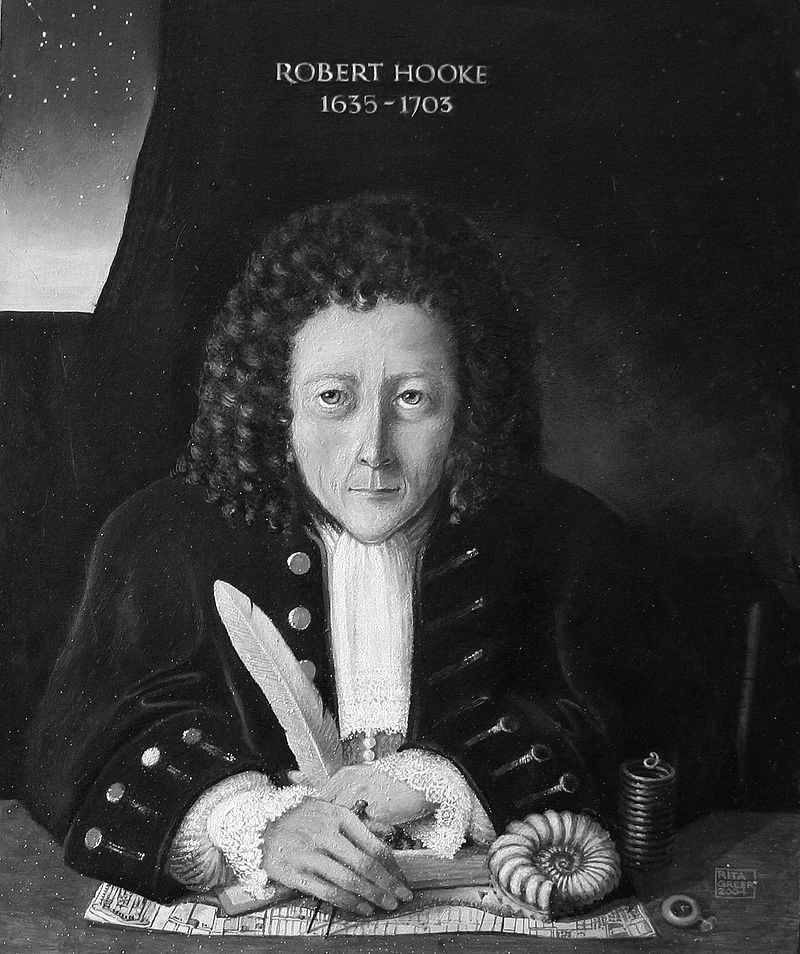
\includegraphics[width=\linewidth]{hooke.jpg}
  \caption{Portrait of Robert Hooke.}
  \label{fig:marginfig}
\end{marginfigure}
\marginnote{As no contemporary portrait of Robert Hooke seems to have survived from the seventeenth century, this one is a reconstruction from the descriptions by his colleagues Aubrey and Waller. It shows him with a spring, pocket watch, fossil and map of the City of London after the Great Fire of 1666. He helped to survey and plan the rebuilding. The sky on the left indicates his interest in astronomy.}


\section{Simple Harmonic Motion}
\subsection{Hooke's Law}

Hooke's law represents a linear restoring force to a point of equilibrium.  This is a model for the ideal spring.  The constant of proportionality, $k$, between the force and displacement is called the spring constant.  For other linear systems $k$ is used to represent the constant of proportionality and simply referred to as the $k$ constant.
$$F_{spring}=-kx$$
This physical system behaves according to a differential kinematic relationship.  Specifically the acceleration has a negative proportionality to the position.
$$F_{spring}=F_{net}=ma$$
$$m \lim_{\Delta \rightarrow 0} \frac{\Delta v}{\Delta t}=-kx$$
$$\lim_{\Delta \rightarrow 0} \frac{\Delta (\Delta x / \Delta t)}{\Delta t}=-\frac{k}{m}x$$
$$a=-\frac{k}{m}x$$

\begin{marginfigure}%

\begin{tikzpicture}[scale=0.6]
	\tikzstyle{spring}=[thick,decorate,decoration={zigzag,pre length=0.1cm,post length=0.1cm,segment length=6}]
	\draw[->,thick] (0,0) -- (0,1) node [anchor=south ,scale=1] {$F_{spring}$}; 
    	\fill[black] (0,0) circle (0.5mm);
	   
	\begin{scope}[shift={(-5,-1)}, scale=0.5]
		\draw[dashed, color=gray] (-3,2) -- (3,2) node [near start, anchor =south east] {\tiny equilibrium};
		\draw[spring] (0,1) -- (0,5);
		\draw[->,thick, color=gray] (2,2) -- (2,0) node [midway, anchor =west] {\small$\overrightarrow{x}$};
		\fill[color=gray!30, path fading=north] (-3,5) -- (3,5) -- (3,7) -- (-3,7) ;
		\draw[very thick] (-3,5) -- (3,5);  
		\draw[very thick] (-1,-1) -- (-1,1) -- (1,1) -- (1,-1) -- cycle;  	 
		\draw (0,0) node [anchor=center]{$m$};
   	 \end{scope}
   
   
   	  \begin{scope}[shift={(-2,0.2)}, scale=0.75, rotate=180] 
	  	\draw[ thick,-stealth] (0,-0.1) -- (0,0.8) node [near start,anchor=east]{\scriptsize $x$};  
	 	 \draw[thick](-0.1,0) -- (0.1,0);  
	  \end{scope}
	  
   \end{tikzpicture}
 
  \caption{Hookean system}
  \label{fig:marginfig}
\end{marginfigure}

   
\subsection{Equations of Motion}
$$x(t)=A\cos(\omega t)+B\sin(\omega t)$$
$$v(t)=-\omega A\sin(\omega t)+\omega B\cos(\omega t)$$
$$A=x_0\ \ \ \ \ \ B=\frac{v_0}{\omega}\ \ \ \ \ \ \omega=\sqrt{\frac{k}{m}}$$
\newpage
\subsection{Energy}
\begin{fullwidth}
The classical harmonic oscillator is a lovely system in terms of symmetry.  Kinetic and potential anergy have equal influence over the evolution of the system.  The inertial quantity $m$ weights the squared velocity to constitute the kinetic energy whereas the elastic quantity $k$ weights the squared distance to constitute the potential energy.

$$KE=\frac{mv^2}{2}\hspace{2cm}PE=\frac{kx^2}{2}$$
$$E=KE+PE$$
$$E=E_0=\frac{mv_0^2}{2}+\frac{kx_0^2}{2}=KE_{max}=PE_{max} \hspace{2cm} KE=E_0-PE=E_0 (\sin^2(2\omega t+\phi) ) $$
$$|v_{max}|=\sqrt{\frac{2E_0}{m}} \hspace{2cm} |x_{max}|=\sqrt{\frac{2E_0}{k}}$$


\section{Pendulum}

\footnotesize{

A pendulum is a weight suspended from a pivot so that it can swing freely.  When a pendulum is displaced sideways from its resting, equilibrium position, it is subject to a restoring force due to gravity that will accelerate it back toward the equilibrium position. When released, the restoring force combined with the pendulum's mass causes it to oscillate about the equilibrium position, swinging back and forth. The time for one complete cycle, a left swing and a right swing, is called the period. The period depends on the length of the pendulum, and also to a slight degree on the amplitude, the width of the pendulum's swing.}

\end{fullwidth}

\vspace{1cm}
\footnotesize{
Newton's second law for rotation of rigid bodies written below.  The net torque is equal to the product of the moment of inertia and the angular acceleration. }
$$\tau_{net}=I\alpha$$
\footnotesize{Substituting the torque and moment of inertia yields the following equation.}
$$mgl\sin{\theta}=ml^2\alpha$$
\footnotesize{The underlying differential relationship of the system is that the double time rate of change of the angle is the ratio of the restoring torque and the inertial moment.}
$$\lim_{\Delta \rightarrow 0} \frac{\Delta^2 \theta}{(\Delta t)^2}=-\frac{g}{l}\sin\theta$$


\begin{marginfigure}[-6cm]
$$\begin{tikzpicture}[scale=0.7]
   
	  \begin{scope}[shift={(-5,-1)}, scale=0.5]
	   \begin{scope}[shift={(1.5,5)}, scale=1, rotate=-20]
	    \draw[very thick] (0,0) -- (0,-5) node [midway, anchor=north east, scale=1] {$l \ \  $}; 
	     \draw[very thick] (0,-6) circle (1cm); 
	     \draw (0,-6) node [anchor=center]{$m$};
	   \end{scope}
	 
	   \draw[dashed] (1.5,5) -- (1.5,1.5) node [midway, anchor=north east] {\small$\theta$};; 
	  \fill[color=gray!30, path fading=north] (-3,5) -- (3,5) -- (3,7) -- (-3,7) ;
	  \draw[very thick] (-3,5) -- (3,5);  
	   
   	
   \end{scope}
   
   
   	  \begin{scope}[shift={(-2,0.2)}, scale=0.75, rotate=-20] 
	  \draw[ thick,-stealth] (0,-0.1) -- (0,0.8) node [near start,anchor=east]{\scriptsize $r$};  
	  \draw[thick](-0.1,0) -- (0.1,0);
	   \draw[thick](0.2,-0.4) -- (0.2,-0.6);
	    \draw[ thick,-stealth] (0.1,-0.5) -- (1,-0.5) node [near start,anchor=north]{\scriptsize $\theta$};  
	  \end{scope}
   \end{tikzpicture}$$


  \caption{Ideal pendelum}
  \label{fig:marginfig}
\end{marginfigure}

\begin{fullwidth}
\footnotesize{
From its examination in around 1602 by Galileo Galilei, the regular motion of pendulums was used for timekeeping, and was the world's most accurate timekeeping technology until the 1930s.  Pendulums are used to regulate pendulum clocks, and are used in scientific instruments such as accelerometers and seismometers. Historically they were used as gravimeters to measure the acceleration of gravity in geophysical surveys, and even as a standard of length. The word "pendulum" is new Latin, from the Latin pendulus, meaning 'hanging'.  The simple gravity pendulum is an idealized mathematical model of a pendulum.  This is a weight (or bob) on the end of a massless cord suspended from a pivot, without friction. When given an initial push, it will swing back and forth at a constant amplitude. Real pendulums are subject to friction and air drag, so the amplitude of their swings declines.
}
\end{fullwidth}

\vspace{1cm}

\subsection{Small Angle Approximation}
$$\sin \theta=\sum_{n=0}^{\infty} \frac{(-1)^n\theta^{2n+1}}{(2n+1)!}=\theta-\frac{\theta^3}{3!}+\frac{\theta^5}{5!}-\cdots$$
$$\lim_{\theta \rightarrow 0} \sin \theta \approx \theta$$

$$\lim_{\Delta \rightarrow 0} \frac{\Delta (\Delta \theta / \Delta t)}{\Delta t}\approx-\frac{g}{l}\theta$$

\marginnote[-4cm]{   
\subsection{Equations of Motion}
$$\Theta(t)=A\cos(\omega t)+B\sin(\omega t)$$
$$\Omega(t)=-\omega A\sin(\omega t)+\omega B\cos(\omega t)$$
$$A=\theta_0\ \ \ \ \ \ B=\frac{\dot{\theta}_0}{\omega}\ \ \ \ \ \ \omega=\sqrt{\frac{g}{l}}$$


\section{Magnitude and Phase}
$$A\cos(t)+B\sin(t)=R\cos(t+\phi)$$
$$R=\sqrt{A^2 + B^2} \hspace{2cm} \phi=\tan^{-1}\left(\frac{B}{A}\right)$$
}

\section{Damped Harmonic Oscillator}
\normalsize
The differential equation that represents the simple harmonic oscillator system is written below.
$$ma=-fx \hspace{2cm} ma+kx=0$$
This equations gives the following solution.
$$x(t)=A\cos(\omega t)+B\sin(\omega t) $$
The dampening occurs when a force is introduced that is proportional to the velocity.  This is the dampening force.
$$ma=-\beta v-kx$$

\chapter{Thermodynamics}

\begin{marginfigure}%
  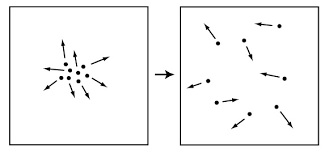
\includegraphics[width=\linewidth]{entrope.jpg}
  \caption{Entropy is the monster of time}
  \label{fig:marginfig}
\end{marginfigure}


\textit{Only entropy comes easy.}  \\
\noindent\textbf{-   Anton Chekov}

\

\marginnote{

\begin{description}
\item[Thermodynamics] 
Thermodynamics is the branch of physics concerned with heat and temperature and their relation to energy and work.  It describes macroscopic variables of systems which are subject to general constraints, common to all materials, expressed in the four laws of thermodynamics.

\item[Heat]
Heat is energy that is transferred between a system and its surroundings, apart from work or or mass transfer.  When there is a suitable physical pathway, heat flows from a hotter temperature to a colder temperature body.  The pathway can be direct, as in conduction and radiation, or indirect, as in convective circulation.
\item[Temperature]
Temperature is the degree or intensity of heat in a substance.  Abstractly, it may be considered a representation of the random activity in a system.  

\item[Celsius] Celsius is a unit of temperature.  One degree Celsius represents the temperature change of one gram of water when $2.39\times10^{-5}\text{Joules}$ of heat is added to it.  It is offset so that the triple point of water is at zero degrees.

\item[Kelvin] Kelvin is a unit of temperature equivalent to Celsius except that its offset is such that the triple point of water is at 273.15 degrees.

\item[Thermal Equilibrium]
Thermal equilibrium is a condition where two substances in physical contact with each other exchange no net heat energy.  Substances in thermal equilibrium are at the same temperature.
\end{description}
}
\section{Systems and States}

\newthought{A thermodynamic system can be defined} in terms of its macroscopic states. In this way, a thermodynamic system is a macroscopic physical object, explicitly specified in terms of macroscopic physical variables that describe its macroscopic properties. 
A thermodynamic system is not simply a physical system.  Rather, in general, indefinitely many different alternative physical systems with specific microscopic states comprise a given thermodynamic system, because in general a physical system has vastly many more detailed characteristics than are mentioned in a thermodynamic description.

For example a system of 1000 particles could be described thermodynamically by the average kinetic energy of the particles.  This would be a thermodynamic state variable.  The actual microscopic state of each of the 1000 particles, each position and velocity at any instant would not be fully determined by the macroscopic variable.  The relationship between macro states and micro states is important in statistical mechanics, an approach to thermodynamics.



\section{History}
\newthought{Historically, the field of thermodynamics} has been the progressive fusion of many different schools of thought.  

Sadi Carnot, the "father of thermodynamics", published Reflections on the Motive Power of Fire (1824), a discourse on heat, power, energy, and engine efficiency. The paper outlined the basic energetic relations between the Carnot engine, the Carnot cycle, and motive power. It marked the start of thermodynamics as a modern science.

The first and second laws of thermodynamics emerged simultaneously in the 1850s, primarily out of the works of William Rankine, Rudolf Clausius, and William Thomson (Lord Kelvin).

\begin{figure}%
\begin{tikzpicture}
\node[inner sep=0pt] (russell) at (0,0)
    {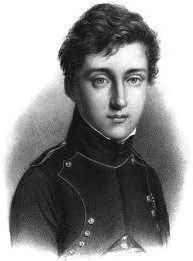
\includegraphics[width=.22\textwidth]{carnot.jpg}};
    \node at (0,2) [anchor = north]{\footnotesize Carnot};
\node[inner sep=0pt] (whitehead) at (3,0)
    {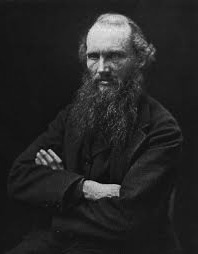
\includegraphics[width=.22\textwidth]{thomson.jpg}};
     \node at (3,2) [anchor = north]{\footnotesize Kelvin};
    \node[inner sep=0pt] (whitehead) at (6,0)
    {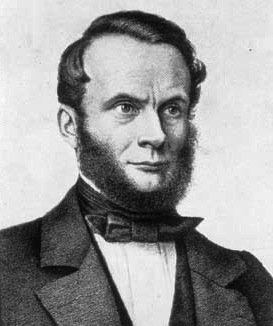
\includegraphics[width=.22\textwidth]{clausius.jpg}};
     \node at (6,2) [anchor = north]{\footnotesize Clausius};
    \node[inner sep=0pt] (whitehead) at (9,0)
    {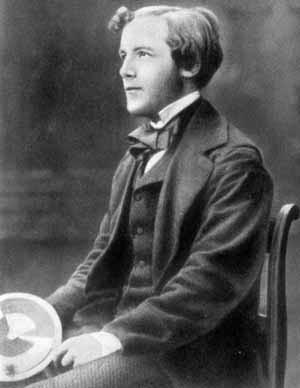
\includegraphics[width=.22\textwidth]{maxwell.jpg}};
     \node at (9,2) [anchor = north]{\footnotesize Maxwell};
      \node[inner sep=0pt] (whitehead) at (0,-4)
    {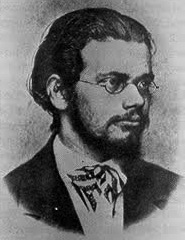
\includegraphics[width=.22\textwidth]{boltzmann.jpg}};
     \node at (0,-2) [anchor = north]{\footnotesize Boltzmann};
    \node[inner sep=0pt] (whitehead) at (3,-4)
    {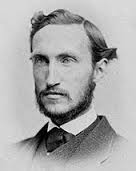
\includegraphics[width=.22\textwidth]{gibbs.jpg}};
     \node at (3,-2) [anchor = north]{\footnotesize Gibbs};
      \node[inner sep=0pt] (whitehead) at (6,-4)
    {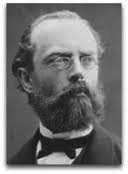
\includegraphics[width=.22\textwidth]{zeuner.jpg}};
     \node at (6,-2) [anchor = north]{\footnotesize Zeuner};
      \node[inner sep=0pt] (whitehead) at (9,-4)
    {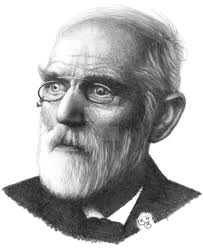
\includegraphics[width=.22\textwidth]{waals.jpg}};
     \node at (9,-2) [anchor = north]{\footnotesize van der Waals};
%\draw[<->,thick] (russell.south east) -- (whitehead.north west)
    %node[midway,fill=white] {Principia Mathematica};
\end{tikzpicture}
  \caption{Many founders of thermodynamics have beards}
  \label{fig:marginfig}
\end{figure}


The foundations of statistical thermodynamics were set out by physicists such as James Clerk Maxwell, Ludwig Boltzmann, Max Planck, Rudolf Clausius and J. Willard Gibbs.  It provided a theoretical explanation for  classical thermodynamics.

American mathematical physicist Josiah Willard Gibbs showed how thermodynamic processes could include chemical reactions. By studying the energy, entropy, volume, chemical potential, temperature and pressure of the thermodynamic system, one can determine whether a chemical process would occur spontaneously.

\marginnote[-150pt]{
\section{Laws of Thermodynamics}
\begin{description}
\item[Zeroth Law]  If two systems are in thermal equilibrium respectively with a third system, they must be in thermal equilibrium with each other. This law helps define the notion of temperature.
\item[First Law]  When energy passes, as work, as heat, or with matter, into or out from a system, its internal energy changes in accord with the law of conservation of energy. Equivalently, perpetual motion machines of the first kind are impossible.
\item[Second Law]  In a natural thermodynamic process, the sum of the entropies of the interacting thermodynamic systems increases. Equivalently, perpetual motion machines of the second kind are impossible.
\item[Third Law]  The entropy of a system approaches zero as the temperature approaches absolute zero and is equal to the log of the multiplicity of the quantum ground states.
\end{description}}




\section {Zeroth Law}
Two systems are said to be in the relation of thermal equilibrium if they are linked by a wall permeable only to heat, and do not change over time.  Thermal equilibrium is transitive.  If two systems are in thermal equilibrium with a third system, then they are in thermal equilibrium with each other.   Systems at thermal equilibrium are at the same temperature.


\newpage

\section {Thermal Expansion}

\marginnote{
$$\alpha=\frac{1}{L_0}\frac{\Delta L}{\Delta T} $$
\vspace{10pt}
$$\beta=\frac{1}{V_0}\frac{\Delta V}{\Delta T} $$}

\newthought{Thermal expansion} is the tendency of matter to change in shape, area, and volume in response to a change in temperature, through heat transfer.  When a substance is heated, the kinetic energy of its molecules increases and maintain a greater average separation.  The fractional expansion divided by the change in temperature is called the material's coefficient of thermal expansion and generally varies with temperature.
            
\begin{margintable}[50pt]\index{typefaces!sizes}
  \footnotesize%
  \begin{center}
    \begin{tabular}{lr}
      \toprule
     Material & Linear Coefficient $\alpha$\\
      \midrule
    Aluminum    & 23.1 $\nicefrac{\mu}{\text{K}}$  \\
    Brass      & 19 $\nicefrac{\mu}{\text{K}}$  \\
    Carbon Steel      & 10.8 $\nicefrac{\mu}{\text{K}}$  \\
     Concrete   & 12 $\nicefrac{\mu}{\text{K}}$  \\
    Copper    & 17 $\nicefrac{\mu}{\text{K}}$  \\
    Iron    & 11.8 $\nicefrac{\mu}{\text{K}}$  \\
   Lead      & 29 $\nicefrac{\mu}{\text{K}}$  \\
    Mercury     & 61 $\nicefrac{\mu}{\text{K}}$  \\
    PVC    & 52 $\nicefrac{\mu}{\text{K}}$  \\
    Water     & 69 $\nicefrac{\mu}{\text{K}}$  \\
      \bottomrule
    \end{tabular}
  \end{center}
  \caption{Coefficients of linear expansion for various materials at $20{}^\circ\text{C}$.}
  \label{tab:font-sizes}
\end{margintable}
           
            
\subsection{Linear Expansion}
The change in the length of some object is the product of the original length, $L_0$, the change in temperature, $\Delta T$, and the coefficient of linear expansion, $\alpha$.
$$\Delta L=\alpha L_0 \ \Delta T $$
The coefficient of linear expansion is an intensive property of the material and changes with temperature.  It can even be negative for exotic materials.
\subsection{Volumetric Expansion}



Volumetric expansion is more appropriate for liquids and gases.  
$$\Delta V=\beta V_0 \ \Delta T $$
The coefficient of volumetric expansion is three times the coefficient of linear expansion.
$$\beta=3\alpha$$

\marginnote[-30pt]{The small calorie or gram calorie is the approximate amount of energy needed to raise the temperature of one gram of water by one degree Celsius at a pressure of one atmosphere.
\vspace{10pt}

$$1 \text{cal}\equiv 4.184 \text{J}$$}

\vspace{1cm}

\section{Specific Heat Capacity}

\begin{margintable}[10pt]\index{typefaces!sizes}
  \footnotesize%
  \begin{center}
    \begin{tabular}{lr}
      \toprule
     Material & Specific Heat\\
      \midrule
      Air     & 1.0 $\nicefrac{\text{kJ}}{\text{kg}\cdot\text{K}}$  \\
    Aluminum    & 0.087 $\nicefrac{\text{kJ}}{\text{kg}\cdot\text{K}}$  \\
    Argon     & 0.520 $\nicefrac{\text{kJ}}{\text{kg}\cdot\text{K}}$  \\
     Concrete   & 0.880  $\nicefrac{\text{kJ}}{\text{kg}\cdot\text{K}}$  \\
    Copper    & 0.385 $\nicefrac{\text{kJ}}{\text{kg}\cdot\text{K}}$  \\
    Iron    & 0.450 $\nicefrac{\text{kJ}}{\text{kg}\cdot\text{K}}$  \\
   Lead      & 0.129 $\nicefrac{\text{kJ}}{\text{kg}\cdot\text{K}}$  \\
    Mercury     & 0.140 $\nicefrac{\text{kJ}}{\text{kg}\cdot\text{K}}$  \\
    Water - Ice    & 2.05 $\nicefrac{\text{kJ}}{\text{kg}\cdot\text{K}}$  \\
    Water - Liquid     & 4.184 $\nicefrac{\text{kJ}}{\text{kg}\cdot\text{K}}$  \\
    Water - Vapor     & 2.00 $\nicefrac{\text{kJ}}{\text{kg}\cdot\text{K}}$  \\
      \bottomrule
    \end{tabular}
  \end{center}
  \caption{Specific heat capacities}
  \label{tab:font-sizes}
\end{margintable}
\newthought{Heat capacity} or thermal capacity is a measurable physical quantity equal to the ratio of the heat added to an object to the resulting temperature change.  The specific heat capacity is the heat capacity per unit mass of a material.  It is often referred to as the specific heat.
$$Q=mC \Delta T$$
$Q$ is the heat added to the system, $m$ is the mass, $C$ is the specific heat capacity and  $\Delta T$ is the change in temperature.
%$$Q=m\int _{T_i}^{T_f}c(T)\  dT$$

\newpage

\section{Latent Heat}
\begin{margintable}[0pt]\index{typefaces!sizes}
  \footnotesize%
  \begin{center}
    \begin{tabular}{lrr}
      \toprule
     Material & $L_{fusion}$&$L_{vapor}$ \\
      \midrule
    Ammonia    &  332 $\nicefrac{\text{kJ}}{\text{kg}}$ &  1369 $\nicefrac{\text{kJ}}{\text{kg}}$  \\
 Carbon Dioxide      &  184 $\nicefrac{\text{kJ}}{\text{kg}}$ &  574 $\nicefrac{\text{kJ}}{\text{kg}}$  \\
    Ethanol   &  108 $\nicefrac{\text{kJ}}{\text{kg}}$ &  855 $\nicefrac{\text{kJ}}{\text{kg}}$  \\
     Hydrogen   &  58 $\nicefrac{\text{kJ}}{\text{kg}}$ & 455 $\nicefrac{\text{kJ}}{\text{kg}}$ \\
   Lead      &  23.0 $\nicefrac{\text{kJ}}{\text{kg}}$&  871 $\nicefrac{\text{kJ}}{\text{kg}}$  \\
    Nitrogen    &  25.7 $\nicefrac{\text{kJ}}{\text{kg}}$&  200 $\nicefrac{\text{kJ}}{\text{kg}}$  \\
    Oxygen    &  13.9 $\nicefrac{\text{kJ}}{\text{kg}}$&  213 $\nicefrac{\text{kJ}}{\text{kg}}$  \\
    Water     &  334 $\nicefrac{\text{kJ}}{\text{kg}}$&  2265 $\nicefrac{\text{kJ}}{\text{kg}}$ \\
      \bottomrule
    \end{tabular}
  \end{center}
  \caption{Latent heats of fusion and vaporization}
  \label{tab:font-sizes}
\end{margintable}

Latent heat is energy released or absorbed, by a body or a thermodynamic system, during a constant-temperature process that is specified in some way. An example is latent heat of fusion for a phase change, melting, at a specified temperature and pressure.

The term was introduced around 1762 by Scottish chemist Joseph Black. It is derived from the Latin \textit{latere} (to lie hidden). Black used the term in the context of calorimetry where a heat transfer caused a volume change while the thermodynamic system's temperature was constant.

$$Q=mL$$

$Q$ is the heat added in the phase change, $m$ is the mass of the material and $L$ is the latent heat.



\section {Ideal Gas}
\begin{marginfigure}[50pt]
  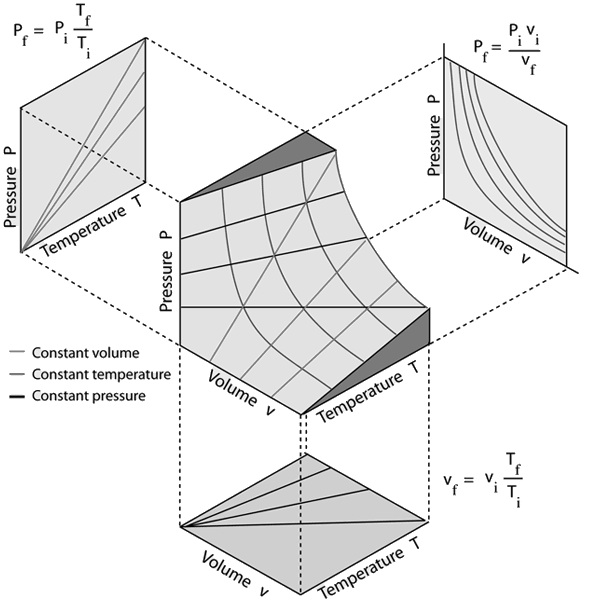
\includegraphics[width=\linewidth]{pvt.jpg}
  \caption{Ideal gas dimensions of pressure, volume and temperature}
  \label{fig:marginfig}
\end{marginfigure}


\marginnote[0pt]{
\newthought{In statistical mechanics} the following molecular equation is derived from first principles.  It is another form of the ideal gas law.  
$$PV=Nk_BT$$
Here $N$ represents the number of particles and $k_B$ is the Boltzmann constant. 
$$k_B=1.38\times 10^{-23} \ \frac{\text{J}}{\text{K}}$$
Taking the two forms of the ideal gas law allows the relation between the gas constant and Boltzmann constant.
$$R=k_B N_A$$
Their ratio is Avogado's number, the number of particles in a mol.
$$N_A=6.02\times10^{23} \frac{1}{\text{mol}}$$
}

An ideal gas is a theoretical gas composed of many randomly moving point particles that do not interact except when they collide elastically. The ideal gas concept is useful because it obeys the ideal gas law, a simplified equation of state, and is amenable to analysis under statistical mechanics. One mole of an ideal gas has a volume of 22.7 L at STP as defined by IUPAC.

At normal conditions such as standard temperature and pressure, most real gases behave qualitatively like an ideal gas. Many gases such as nitrogen, oxygen, hydrogen, noble gases, and some heavier gases like carbon dioxide can be treated like ideal gases within reasonable tolerances.

\subsection{Ideal Gas Law}
The ideal gas law is the equation of state of a hypothetical ideal gas. It is a good approximation to the behavior of many gases under many conditions, although it has several limitations. It was first stated by Emile Clapeyron in 1834 as a combination of Boyle's law, Charles's law and Avogadro's Law.

$$PV=nRT$$

Here $P$ is the pressure, $V$ is the volume, $n$ is the number of moles of gas, $R$ is the gas constant and $T$ is the temperature.

$$R=8.31 \ \frac{\text{J}}{\text{mol}\cdot \text{K}}$$

\newpage

\subsection{Coefficient of Volumetric Expansion}
Beginning with the molecular ideal gas law, the coefficient of volumetric expansion $\beta$, may be derived.
$$PV=Nk_BT$$
The coefficient of thermal expansion is defined.
$$\beta=\frac{1}{V_0}\frac{\Delta V}{\Delta T} $$
Use of the ideal gas law yields the derived coefficient $\beta$.
$$\beta=\frac{N}{V_0}\frac{k_B}{P} $$

\subsection{Kinetic Theory}
\marginnote[-230pt]{
\subsection{Internal Energy}
The punchline of kinetic theory's model of the monatomic ideal is more than a model for pressure.  Kinetic theory gives the insight that the product of pressure and volume is proportional to the kinetic energy of the particles.
$$PV=\frac{2}{3}N \braket{KE}_{particle}=\frac{2}{3} \braket{KE}_{system}$$
Combine this with the molecular form of the ideal gas law.
$$PV=Nk_BT$$
This reveals the relationship between temperature and internal kinetic energy.
$$k_BT=\frac{2}{3} \braket{KE}_{particle}$$
Writing the total internal kinetic energy of the system $U$ yields the following.
$$U=\frac{3}{2} N k_B T$$
Temperature is a measure of the internal kinetic energy of a system. 

\subsection{Specific Heat}
The specific heat capacity of an ideal gas may be derived directly.
$$C=\frac{1}{m}\frac{\Delta U}{\Delta T}=\frac{3}{2} \frac{N}{m} k_B$$
$$C=\frac{3}{2}\frac{ k_B}{m_{part}}$$}

\marginnote{
\subsection{Equipartition of Energy}
Each degree of freedom contributes, on the average, $\frac{k_BT}{2}$ of energy per molecule.  For a monatomic ideal gas there are three translational degrees of freedom.  For a diatomic ideal gas there are two degrees of rotational freedom and three degrees of translational freedom.
\subsection{Statistical Distributions}
Boltzmann 
$$N(E)=N_0e^{\frac{-E}{k_BT}}$$
Maxwell-Boltzmann
$$N_v=4\pi N \left(\frac{m}{2\pi k_b T}\right)^{3/2}v^2e^{\frac{-mv^2}{2k_BT}}$$}

This kinetic theory of a monatomic ideal gas develops the concept of pressure and temperature from the microscopic/molecular view and connects to the ideal gas law.

Consider a particle, mass $m$, in a three-dimensional cube with side length $L$.  In the x spatial dimension the particle would bounce back and forth at a speed equal to the magnitude of the x-component of the velocity, $v_x$.  The particle has a momentum component $p_x$.
 $$p_x=mv_x$$
 On interaction with the wall the particle undergoes an elastic collision and imparts an impulse to the wall equal to twice the magnitude of the momentum in the x direction.
 $$\Delta p=2mv_x$$
 The average force associated with the repeated collision of the particle is determined.
 $$\braket{F}=\frac{\Delta p}{\Delta t}=\frac{2mv_x}{\nicefrac{2L}{v_x}}=\frac{mv_x^2}{L}$$
 With this the pressure may be determined.  
 $$P=\frac{\braket{F}}{A}=\frac{mv_x^2}{L^3}=\frac{mv_x^2}{V}$$
 For particles moving isotropically there is no prefered direction in space and therefore $\braket{v_x^2}=\nicefrac{\braket{v^2}}{3}$.  This yields the following expression for $N$ particles.
 $$PV=\frac{2}{3}N\frac{mv^2}{2}=\frac{2}{3}N \braket{KE}$$





\newpage

\section{Work}
\begin{marginfigure}[0pt]%
  \begin{tikzpicture}
    [line cap=round,line join=round,x=2cm,y=2cm, scale=1.5, decoration={brace,amplitude=2pt}]
%main layer
%creating the ticks and xy-axis nodes
%some function
\fill[fill=red!20] (0.25,0) -- plot [domain=0.25:.75] (\x,{-\x^2/2+\x+0.25}) -- plot [domain=0.75: 0.25] (\x,0) -- cycle;

 \draw[smooth,samples=200,domain=0.25:0.75]
                                 plot(\x,{-\x^2/2+\x+0.25});
 

    \fill[black] (0.25,0) circle (0.3mm) node [anchor=north ,scale=1] {$ V_a$};
     \fill[black] (0.75,0) circle (0.3mm) node [anchor=north ,scale=1] {$V_b$};
      %  \fill[black] (0,0.25) circle (0.3mm) node [anchor=south east,scale=1] {\scriptsize$ v(0)$};

  \draw[-latex,color=black,thin] (-0.2,0) -- (1.4,0) node [anchor=north ,scale=1] {$V$};
   \draw[-latex,color=black,thin] (0,-0.2) -- (0,1.4)node [anchor=east ,scale=1] {$P$};
    \draw (0.6,0.8) node [anchor=south west ,scale=1] {$P(V)$};
        \draw (0.5,0.25) node [anchor=center ,scale=1] {$W$};
        
 \end{tikzpicture}
  \caption{Work is the area under the curve in a pressure versus volume graph.}
  \label{fig:marginfig}
\end{marginfigure}

Consider a gas in a piston chamber with cross sectional area $A$.  The work done by the gas, $W$ is the product of the force on the piston, $F$ and the displacement of the piston $\Delta x$.
$$W=F\Delta x=P A\Delta x=P \Delta V$$
The work done by an expanding gas is equal to the product of pressure and change in volume.  On a pressure vs temperature graph the work is the area under the line.
$$W=\text{Area}(P(V))$$


\section {Ideal Gas}
\begin{marginfigure}[50pt]
  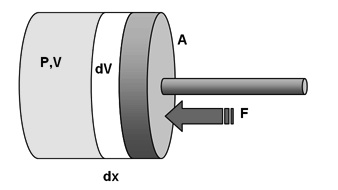
\includegraphics[width=\linewidth]{piston.jpg}
  \caption{Piston chamber}
  \label{fig:marginfig}
\end{marginfigure}
\vspace{1cm}

\section{First Law of Thermodynamics}
The first law of thermodynamics is an energy conservation law.  The internal energy of a gas may be changed though the addition of energy by incoming heat $Q$ or removal or energy by the gas performing work on the surroundings $W$.
$$\Delta U=Q-W$$
For an ideal gas in a piston chamber the following is true.
$$PV=nRT=Nk_BT \hspace{2cm} W=\text{Area}(P(V))$$
Monatomic ideal gas:
$$U=\nicefrac{3}{2} PV$$
Diatomic ideal gas:
$$U=\nicefrac{5}{2} PV$$

\subsection{History}
The process of development of the first law of thermodynamics was by way of much investigative trial and error over a period of about half a century. The first full statements of the law came in 1850 from Rudolf Clausius and from William Rankine.  

Germain Hess in 1840 stated a conservation law for the so-called 'heat of reaction' for chemical reactions.  His law was later recognized as a consequence of the first law of thermodynamics, but Hess's statement was not explicitly concerned with the relation between energy exchanges by heat and work.

\newpage

\subsection{Isothermal Expansion}
\begin{marginfigure}[0pt]%
  \begin{tikzpicture}
    [line cap=round,line join=round,x=2cm,y=2cm, scale=1.5, decoration={brace,amplitude=2pt}]
%main layer
%creating the ticks and xy-axis nodes
%some function

 \draw[smooth,samples=100,domain=0.2:1.2]
                             plot(\x,0.2/\x);

 
  \fill[black] (0.2,1) circle (0.3mm) node [anchor=south ,scale=1] {$ A$};
   \fill[black] (1.2,0.167) circle (0.3mm) node [anchor=south,scale=1] {$ B$};
 
 
 \fill[black] (0,1) circle (0.3mm) node [anchor=east ,scale=1] {$ P_a$};
     \fill[black] (0,0.167) circle (0.3mm) node [anchor=east ,scale=1] {$P_b$};

    \fill[black] (0.25,0) circle (0.3mm) node [anchor=north ,scale=1] {$ V_a$};
     \fill[black] (1.2,0) circle (0.3mm) node [anchor=north ,scale=1] {$V_b$};
      %  \fill[black] (0,0.25) circle (0.3mm) node [anchor=south east,scale=1] {\scriptsize$ v(0)$};

  \draw[-latex,color=black,thin] (-0.2,0) -- (1.4,0) node [anchor=north ,scale=1] {$V$};
   \draw[-latex,color=black,thin] (0,-0.2) -- (0,1.4)node [anchor=east ,scale=1] {$P$};
    \draw (0.6,0.8) node [anchor=south west ,scale=1] {$P(V)_{T=constant}$};
       % \draw (0.5,0.25) node [anchor=center ,scale=1] {$W$};
        
 \end{tikzpicture}
  \caption{Constant Temperature}
  \label{fig:marginfig}
\end{marginfigure}

During isothermal expansion temperature remains constant.
$$T=\text{constant}$$
Under these conditions pressure is inversely proportional to volume.
$$P(V)=\frac{Nk_BT}{V}$$
The work is the area under the $P(V)$ curve.
$$W=Nk_BT \ln \left( \frac{V_b}{V_a}\right)$$
The change in internal energy is given.
$$\Delta U=Q-Nk_BT \ln \left( \frac{V_b}{V_a}\right)$$



\subsection{Isobaric Expansion}
\begin{marginfigure}[70pt]%
  \begin{tikzpicture}
    [line cap=round,line join=round,x=2cm,y=2cm, scale=1.5, decoration={brace,amplitude=2pt}]

\draw[->,color=black,thick] (0.2,1) -- (0.7,1);
\draw[color=black,thick] (0.7,1) -- (1.2,1);
% \draw[->-,color=black,thin] (0.2,1) -- (1.2,1) node [anchor=north ,scale=1] {$V$};


 
  \fill[black] (0.2,1) circle (0.3mm) node [anchor=south ,scale=1] {$ A$};
   \fill[black] (1.2,1) circle (0.3mm) node [anchor=south,scale=1] {$ B$};
 
 
 \fill[black] (0,1) circle (0.3mm) node [anchor=east ,scale=1] {$ P_{a,b}$};
   
    \fill[black] (0.25,0) circle (0.3mm) node [anchor=north ,scale=1] {$ V_a$};
     \fill[black] (1.2,0) circle (0.3mm) node [anchor=north ,scale=1] {$V_b$};
      %  \fill[black] (0,0.25) circle (0.3mm) node [anchor=south east,scale=1] {\scriptsize$ v(0)$};

  \draw[-latex,color=black,thin] (-0.2,0) -- (1.4,0) node [anchor=north ,scale=1] {$V$};
   \draw[-latex,color=black,thin] (0,-0.2) -- (0,1.4)node [anchor=east ,scale=1] {$P$};
    \draw (0.6,0.5) node [anchor=south west ,scale=1] {$P(V)=constant$};
       % \draw (0.5,0.25) node [anchor=center ,scale=1] {$W$};
        
 \end{tikzpicture}
  \caption{Constant Pressure}
  \label{fig:marginfig}
\end{marginfigure}

During isobaric expansion pressure is constant.
$$P=\text{constant} $$
Work is easily computed.
$$ W=P \ \Delta V$$
The change in the internal energy given.
$$\Delta U=Q-P\Delta V$$


\subsection{Isovolumetric Heating}
\begin{marginfigure}[30pt]%
  \begin{tikzpicture}
    [line cap=round,line join=round,x=2cm,y=2cm, scale=1.5, decoration={brace,amplitude=2pt}]
%main layer
%creating the ticks and xy-axis nodes
%some function


\draw[->,color=black,thick] (0.2,1) -- (0.2,0.6);
\draw[color=black,thick] (0.2,0.6) -- (0.2,0.2);
% \draw[->-,color=black,thin] (0.2,1) -- (1.2,1) node [anchor=north ,scale=1] {$V$};


 
  \fill[black] (0.2,1) circle (0.3mm) node [anchor=south ,scale=1] {$ A$};
   \fill[black] (0.2,0.2) circle (0.3mm) node [anchor=north,scale=1] {$ B$};
 
 
 \fill[black] (0,1) circle (0.3mm) node [anchor=east ,scale=1] {$ P_a$};
 \fill[black] (0,0.2) circle (0.3mm) node [anchor=east ,scale=1] {$ P_b$};
   
    \fill[black] (0.2,0) circle (0.3mm) node [anchor=north ,scale=1] {$ V_{a,b}$};
   
      %  \fill[black] (0,0.25) circle (0.3mm) node [anchor=south east,scale=1] {\scriptsize$ v(0)$};

  \draw[-latex,color=black,thin] (-0.2,0) -- (1.4,0) node [anchor=north ,scale=1] {$V$};
   \draw[-latex,color=black,thin] (0,-0.2) -- (0,1.4)node [anchor=east ,scale=1] {$P$};
    \draw (0.6,0.5) node [anchor=south west ,scale=1] {$V=constant$};
       % \draw (0.5,0.25) node [anchor=center ,scale=1] {$W$};
        
 \end{tikzpicture}
  \caption{Constant Volume}
  \label{fig:marginfig}
\end{marginfigure}

During isovolumetric heating the volume is constant.
$$V=\text{constant} $$
Therefore there is no work.
$$W=0$$
This makes the change in internal energy equal to the heat added to the system.
$$\Delta U=Q$$

\subsection{Adiabatic Expansion}
In an adiabatic process there is not heat transferred.
$$Q=0$$
Energy is transferred only as work.
$$\Delta U=-W$$

%\section{Heat Transfer}
%\subsection{Conduction}
%$$H=-kA\frac{dT}{dx}$$
%\subsection{Radiation: Stefan's Law}
%$$P=\sigma A e T^4$$
%$$ e=\text{emissivity} \hspace{2cm} \sigma=5.6696\times 10^{-8} \frac{\text{W}}{\text{m}^2\text{K}^4}$$
%\subsection{Convection}
%In convection the heated substance moves.

\newpage

\section{Heat Engines}
\begin{marginfigure}[0pt]
  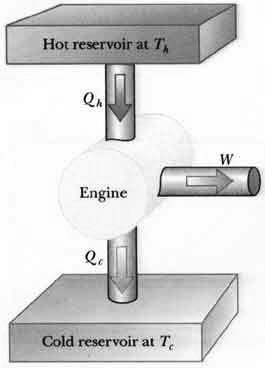
\includegraphics[width=0.75\linewidth]{heat_engine.jpg}
  \caption{Heat engine}
  \label{fig:marginfig}
\end{marginfigure}

Work is done by heat transfer from a hot reservoir to a cold reservoir.

$$\text{Hot reservoir}\ \ \ Q_{in}=Q_h \hspace{2cm} \text{Cold reservoir}\ \ \ Q_{out}=Q_c$$ 
$$Q_{in}>Q_{out}$$
$$W=Q_{in}-Q_{out} \hspace{2cm} W>0$$
Work done by the engine is positive.  The engine is a source of power.
\subsection{Efficiency}
$$e=\frac{W}{Q_{in}}=\frac{Q_{in}-Q_{out}}{Q_{in}}$$
\section{Refrigerator}
\begin{marginfigure}[50pt]
  \includegraphics[width=0.75\linewidth]{refrig.jpg}
  \caption{Refrigerator}
  \label{fig:marginfig}
\end{marginfigure}
Heat is pushed against its temperature gradient from a cold reservoir to a hot reservoir.  
$$\text{Cold reservoir}\ \ \ Q_{in}=Q_c \hspace{2cm} \text{Hot reservoir}\ \ \ Q_{out}=Q_h$$ 
$$Q_{in}>Q_{out}$$
$$W=Q_{in}-Q_{out} \hspace{2cm} W<0$$
Work done by the refrigerator is negative.  Work is done on the refrigerator to increase the temperature gradient.  It requires a source of power.

 \section{Entropy}
 $S$ is the entropy of a system.  For reversible processes:
 $$T=\lim_{\Delta \rightarrow 0} \frac{\Delta Q}{\Delta S}$$
 $$\Delta Q=T \Delta S$$

 Isolated systems tend toward disorder.  Entropy is a measure of this disorder.  The entropy of the universe increases with every \textbf{irreversible} process.


\section{Second Law of Thermodynamics}
Entropy of the universe always stays the same or increases in any thermodynamic process.
\subsection{Kelvin-Plank}
It is \textbf{impossible} to construct a heat engine that, in a cycle, operates to absorb heat $Q_{in}$ and produce an equivalent amount of work, $W=Q_{in}$ so that $Q_{out}=0$.
\subsection{Clausius}
It is \textbf{impossible} to construct a refrigerator that, in a cycle, operates to absorb heat $Q_{in}$ from a cold sink and deliver it to a hot sink, $Q_{out}=Q_{in}$ so that $W=0$.


\section{The Carnot Engine}

\begin{marginfigure}[0pt]
  \includegraphics[width=\linewidth]{carnot_cycle.jpg}
  \caption{Carnot cycle}
  \label{fig:marginfig}
\end{marginfigure}

The Carnot engine is an idealized reversible engine with the maximal efficiency possible between a given hot and cold reservoir. 
\begin{enumerate}
\item Isothermal expansion  (in contact with the heat reservoir, constant temperature)
\item Adiabatic expansion  (thermally isolated, constant entropy)
\item Isothermal compression  (in contact with cold reservoir, constant temperature)
\item Adiabatic compression  (thermally isolated, constant entropy)
\end{enumerate}

 \subsection{Carnot Efficiency}
 $$e_c=\frac{T_h-T_c}{T_h}$$
 

 \subsection{Ideal Gas Reversible Process}
 $$dQ_r=dU+PdV=nC_VdT+nRT\frac{dV}{V}$$
 $$\Delta S=\int_i^f\frac{dQ_r}{T}=nC_V \ln \frac{T_f}{T_i}+nR\ln \frac{V_f}{V_i}$$
 \section{Irreversible Processes}
 \subsection{Free Expansion}
 $$\Delta S=nR\ln \frac{V_f}{V_i}$$
 \subsection{Heat Conduction}
 $$\Delta S=\frac{Q}{T_c}-\frac{Q}{T_h} $$
 \subsection{Heat Transfer}
  $$\Delta S=m_1c_1\ln \frac{T_f}{T_1} + m_2c_2\ln \frac{T_f}{T_2}$$
  
  \section{Third Law of Thermodynamics}
  The third law of thermodynamics is sometimes stated as follows, regarding the properties of systems in equilibrium at absolute zero temperature:
  
  \vspace{1cm}

The entropy of a perfect crystal at absolute zero is exactly equal to zero.

  \vspace{1cm}
  
At absolute zero (zero kelvin), the system must be in a state with the minimum possible energy, and the above statement of the third law holds true provided that the perfect crystal has only one minimum energy state. Entropy is related to the number of accessible microstates, and for a system consisting of many particles, quantum mechanics indicates that there is only one unique state (called the ground state) with minimum energy.
  
  \section{Statistical Mechanics}
  $$P_\beta(\sigma) ={e^{-\beta H(\sigma)} \over Z_\beta} \hspace{2cm} \beta=\frac{1}{k_BT} \hspace{2cm}Z_\beta = \sum_\sigma e^{-\beta H(\sigma)}\hspace{2cm} S=k\ln \Omega$$
 

%\begin{tikzpicture}[scale=0.6]
	\tikzstyle{spring}=[thick,decorate,decoration={zigzag,pre length=0.1cm,post length=0.1cm,segment length=6}]
	\draw[->,thick] (0,0) -- (0,1) node [anchor=south east,scale=1] {$F_{spring}$}; 
    	\fill[black] (0,0) circle (0.5mm);
	   
	\begin{scope}[shift={(-8,-1)}, scale=0.5]
		\draw[dashed, color=gray] (-3,2) -- (3,2) node [near start, anchor =south east] {\tiny equilibrium};
		\draw[spring] (0,1) -- (0,5);
		\draw[->,thick, color=gray] (2,2) -- (2,0) node [midway, anchor =west] {\small$\overrightarrow{x}$};
		\fill[color=gray!30, path fading=north] (-3,5) -- (3,5) -- (3,7) -- (-3,7) ;
		\draw[very thick] (-3,5) -- (3,5);  
		\draw[very thick] (-1,-1) -- (-1,1) -- (1,1) -- (1,-1) -- cycle;  	 
		\draw (0,0) node [anchor=center]{$m$};
   	 \end{scope}
   
   
   	  \begin{scope}[shift={(-2,0.2)}, scale=0.75, rotate=180] 
	  	\draw[ thick,-stealth] (0,-0.1) -- (0,0.8) node [near start,anchor=east]{\scriptsize $x$};  
	 	 \draw[thick](-0.1,0) -- (0.1,0);  
	  \end{scope}
	  
	  
	  \begin{scope}[shift={(-15,0)}, scale=0.5, rotate=45]
		
		\draw[->] (0,0) -- (8,0) node [anchor=north] {$x$};
		\draw[->] (0,0) -- (0,8) node [anchor=east] {$y$};
	 \end{scope}

	  
   \end{tikzpicture}

\vspace{2cm}


\begin{tikzpicture}[scale=0.6]
		   
		   \pgfmathsetseed{10}
		   
	\foreach \x in {0,...,30}
			t = rand
                             \draw[fill] (rand,rand) circle [radius=.5pt];   
                                  \draw[fill] (t,t) circle [radius=.5pt];   
	   
	   
		  
   \end{tikzpicture}





%\bibliography{sample-handout}
%\bibliographystyle{plainnat}


\printindex

\end{document}

